\section{Beam Line and Detectors}
\label{hptpcPaper:sec:Methods}

\subsection{Beam Test Overview}
The beam test took place in the T10 beam line, in the East Area at the Proton Synchrotron (PS) at CERN.
The T10 beamline at CERN is a secondary beam derived from the PS beam which consists primarily of protons, electrons and charged pions~\cite{T10Report}.
%The results in this paper use data taken on the 28th August and 1st September, during which the setup configuration was varied as described below.
The primary components of the experimental setup are shown schematically in Figure~\ref{fig:setup}.

\begin{figure}
  \includegraphics[width=1.0\linewidth]{files/Figures/hptpc_t10_planview.pdf}
  \caption{Schematic diagram (plan view) of the HPTPC beam test configuration in the T10 area at CERN.}
  \label{fig:setup}
\end{figure}
\begin{figure}
  \centering
  \includegraphics[width=1.0\linewidth]{files/Figures/S1S2S3S4.png}
  \caption{Photos illustrating the ToF constituents. Left: the downstream part of the setup which shows the $\mathit{S3}$, $\mathit{S4}$ detectors and HPTPC. Right: $\mathit{S1}$ and $\mathit{S2}$ counters and the stand with four acrylic moderator blocks.}
  \label{fig:modblocks}
\end{figure}

A beam position monitor (BPM) was situated at the beam entrance into the test area, upstream of all the ToF constituents and the TPC. 
The TPC was placed 13~m downstream of the BPM. 
From initial GEANT4~\cite{brun1993geant} beam simulations, the optimal TPC position was determined to be between 2$^{ \circ }$ and 3$^{ \circ }$ off the beam axis, but space constraints meant the TPC could not be placed that far away from the nominal beam centre. So, the beam was steered approximately 1$^{ \circ }$ away from its nominal position, and the TPC placed 1.5$^{ \circ }$ away from the nominal beam centre so that the TPC active region subtended an off-axis angular range of 1.4--3.8$^{ \circ }$.

There were four ToF constituents: 
\begin{itemize}
    \item $\mathit{S1}$, a small-area beam trigger, see Section~\ref{subsec:s1s2Exp};
    \item $\mathit{S2}$, a coincidence measurement with $\mathit{S1}$, see Section~\ref{subsec:s1s2Exp};
    \item $\mathit{S3}$, a wall of plastic scintillator bars placed directly upstream of the TPC vessel, see Section~\ref{subsec:s3Exp};
    \item $\mathit{S4}$, a wall of plastic scintillator bars placed directly downstream of the TPC vessel, see Section~\ref{subsec:s4Exp}.
\end{itemize}

A series of acrylic (polymethyl methacrylate) blocks was placed between the $\mathit{S1}$ and $\mathit{S2}$ counters.
Up to four $10\times10\times10$~cm$^3$ acrylic blocks could be placed contiguously on a tripod stand.
Figure~\ref{fig:modblocks} shows the stand with four blocks installed.
The moderator blocks have the effect of both reducing the energies of incoming particles as well as changing their directions.
This tends to increase the proton-to-MIP ratio at low off-axis angles from the beam, while decreasing the total number of protons and MIPs traversing the TPC.
Data were collected with the T10 beam momentum setting at 0.8~GeV/c, and with each configuration of 0 to 4 moderator blocks.

%The ToF systems were placed in off-axis positions with respect to the direction of the beam to match the TPC position.
The data acquisition (DAQ) systems of the $\mathit{S3}$ (upstream) and $\mathit{S4}$ (downstream) ToF systems were completely independent.
Synchronization between ToF DAQ systems was performed offline using the reference signal from the PS at the beginning of every spill.
T10 received 1--3 spills from the PS during each supercycle, which has a typical duration of 33~s.
The spill duration is 400~ms.
The minimum separation in time between two spills is 1 second, so the start-of-spill signal frequency is less than or equal to 1~Hz.
The trigger condition of the upstream ToF was based on the coincidence between $\mathit{S1}$ and $\mathit{S3}$ constituents.
$\mathit{S2}$ signals were also recorded by the upstream ToF DAQ but were not used in the trigger.
The DAQ of the downstream ToF was run in self-triggering mode with a gate open during the spill.
Coincidence signals between $\mathit{S1}$ and $\mathit{S2}$ counters were also recorded by the downstream ToF DAQ and were used in the particle identification (PID) analysis, described in Section~\ref{hptpcPaper:sec:Results}.  

\subsection{Survey and coordinate system}
\label{sec:coord}
The T10 beamline area was surveyed, and the distances to specific components measured with a precision of 0.5~mm by the CERN Survey, Mechatronics and Measurements (SMM) group.
Multiple points on each of $\mathit{S1}$, $\mathit{S2}$, $\mathit{S3}$, $\mathit{S4}$ and the TPC frame have had their positions measured.

The axes of a right-handed coordinate system are defined as follows: $\hat{x}$ refers to the non-beam horizontal direction, $\hat{y}$ to the vertical direction, and $\hat{z}$ the beam direction, as shown in Figure~\ref{fig:setup}.
We show results in terms of two off-axis angles: $\theta$, which is measured in the $\hat{x}-\hat{z}$ plane with positive angles measured in the $+\hat{x}$ direction, and $\phi$, which is measured in the $\hat{y}-\hat{z}$ plane with positive angles measured in the $+\hat{y}$ direction.
The origin is taken to be at $\mathit{S1}$.

Figure~\ref{fig:angularDistS1} shows the angular extent of objects within the beamline using the coordinate system defined above.
Table~\ref{tab:angS1} shows the calculated angular extent of the various beamline components as measured from $\mathit{S1}$.
Table~\ref{tab:distances} shows the distances between the centres of various objects in the T10 beamline.
These distances were calculated using the data gathered by the survey team.

\begin{figure}[ht]
  \begin{adjustbox}{max totalsize={0.7\textwidth}{.5\textheight},center}
    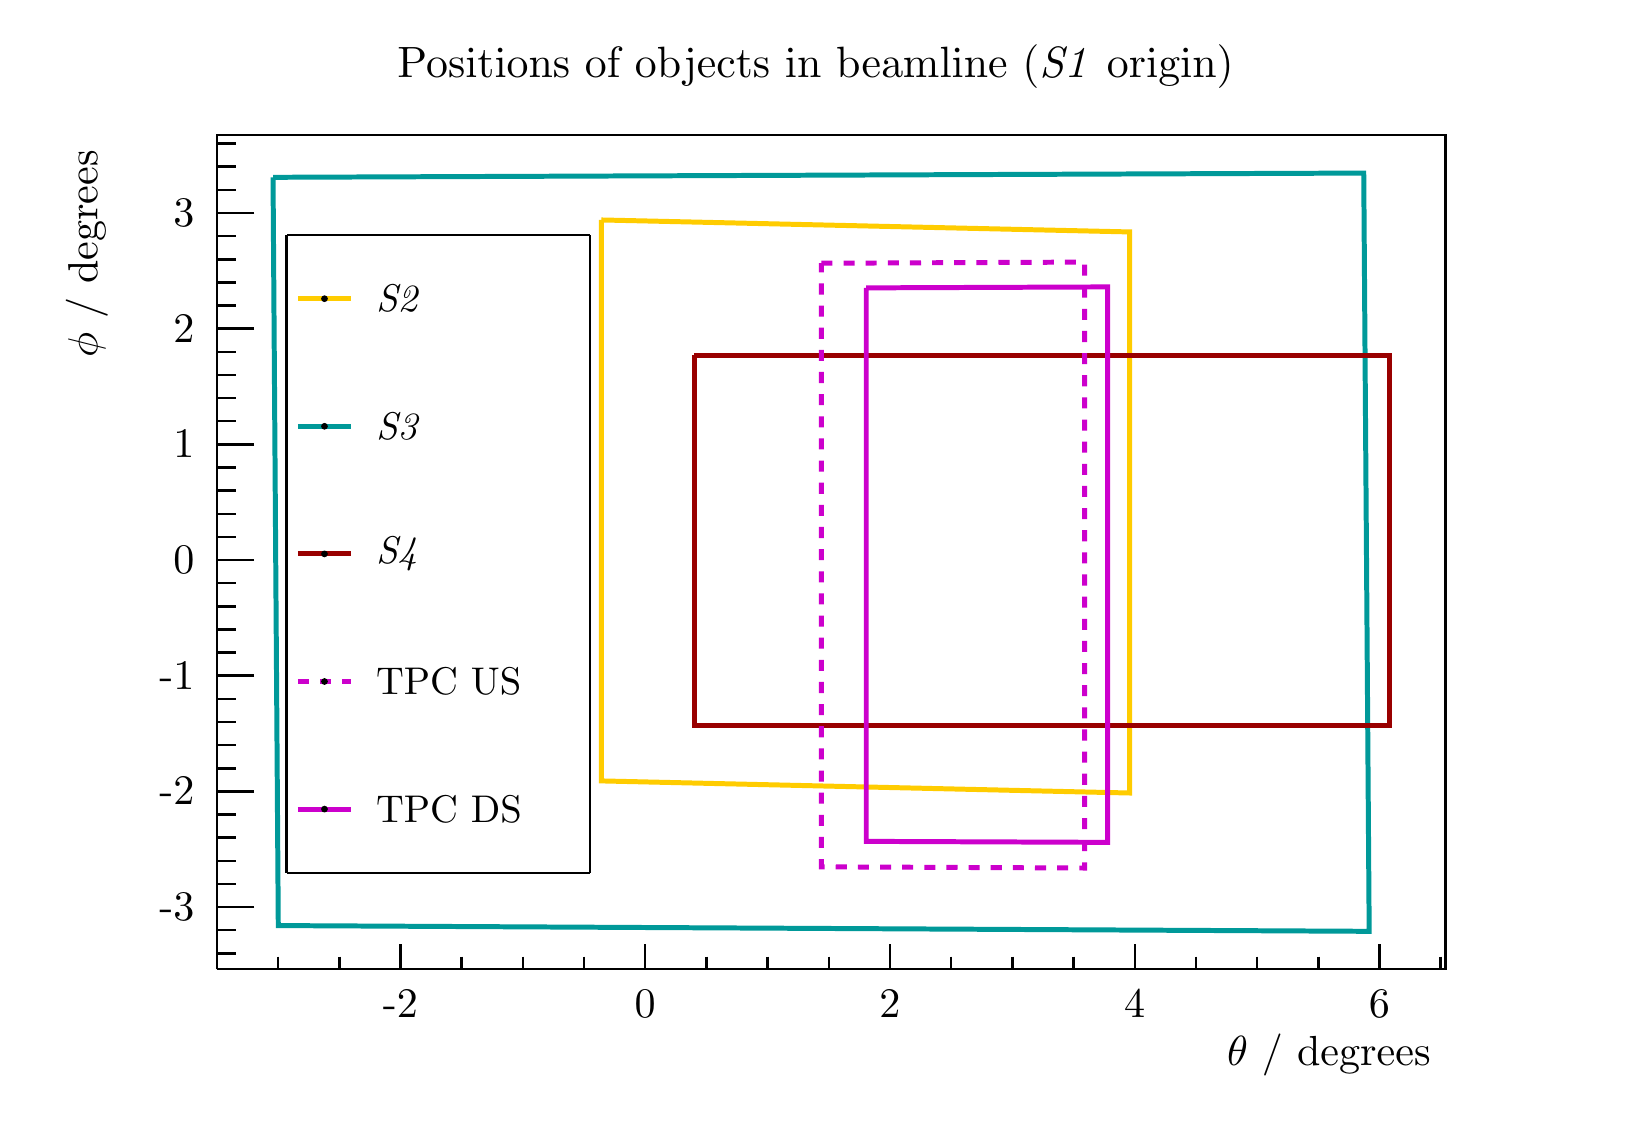
\begin{tikzpicture}
\pgfdeclareplotmark{cross} {
\pgfpathmoveto{\pgfpoint{-0.3\pgfplotmarksize}{\pgfplotmarksize}}
\pgfpathlineto{\pgfpoint{+0.3\pgfplotmarksize}{\pgfplotmarksize}}
\pgfpathlineto{\pgfpoint{+0.3\pgfplotmarksize}{0.3\pgfplotmarksize}}
\pgfpathlineto{\pgfpoint{+1\pgfplotmarksize}{0.3\pgfplotmarksize}}
\pgfpathlineto{\pgfpoint{+1\pgfplotmarksize}{-0.3\pgfplotmarksize}}
\pgfpathlineto{\pgfpoint{+0.3\pgfplotmarksize}{-0.3\pgfplotmarksize}}
\pgfpathlineto{\pgfpoint{+0.3\pgfplotmarksize}{-1.\pgfplotmarksize}}
\pgfpathlineto{\pgfpoint{-0.3\pgfplotmarksize}{-1.\pgfplotmarksize}}
\pgfpathlineto{\pgfpoint{-0.3\pgfplotmarksize}{-0.3\pgfplotmarksize}}
\pgfpathlineto{\pgfpoint{-1.\pgfplotmarksize}{-0.3\pgfplotmarksize}}
\pgfpathlineto{\pgfpoint{-1.\pgfplotmarksize}{0.3\pgfplotmarksize}}
\pgfpathlineto{\pgfpoint{-0.3\pgfplotmarksize}{0.3\pgfplotmarksize}}
\pgfpathclose
\pgfusepathqstroke
}
\pgfdeclareplotmark{cross*} {
\pgfpathmoveto{\pgfpoint{-0.3\pgfplotmarksize}{\pgfplotmarksize}}
\pgfpathlineto{\pgfpoint{+0.3\pgfplotmarksize}{\pgfplotmarksize}}
\pgfpathlineto{\pgfpoint{+0.3\pgfplotmarksize}{0.3\pgfplotmarksize}}
\pgfpathlineto{\pgfpoint{+1\pgfplotmarksize}{0.3\pgfplotmarksize}}
\pgfpathlineto{\pgfpoint{+1\pgfplotmarksize}{-0.3\pgfplotmarksize}}
\pgfpathlineto{\pgfpoint{+0.3\pgfplotmarksize}{-0.3\pgfplotmarksize}}
\pgfpathlineto{\pgfpoint{+0.3\pgfplotmarksize}{-1.\pgfplotmarksize}}
\pgfpathlineto{\pgfpoint{-0.3\pgfplotmarksize}{-1.\pgfplotmarksize}}
\pgfpathlineto{\pgfpoint{-0.3\pgfplotmarksize}{-0.3\pgfplotmarksize}}
\pgfpathlineto{\pgfpoint{-1.\pgfplotmarksize}{-0.3\pgfplotmarksize}}
\pgfpathlineto{\pgfpoint{-1.\pgfplotmarksize}{0.3\pgfplotmarksize}}
\pgfpathlineto{\pgfpoint{-0.3\pgfplotmarksize}{0.3\pgfplotmarksize}}
\pgfpathclose
\pgfusepathqfillstroke
}
\pgfdeclareplotmark{newstar} {
\pgfpathmoveto{\pgfqpoint{0pt}{\pgfplotmarksize}}
\pgfpathlineto{\pgfqpointpolar{44}{0.5\pgfplotmarksize}}
\pgfpathlineto{\pgfqpointpolar{18}{\pgfplotmarksize}}
\pgfpathlineto{\pgfqpointpolar{-20}{0.5\pgfplotmarksize}}
\pgfpathlineto{\pgfqpointpolar{-54}{\pgfplotmarksize}}
\pgfpathlineto{\pgfqpointpolar{-90}{0.5\pgfplotmarksize}}
\pgfpathlineto{\pgfqpointpolar{234}{\pgfplotmarksize}}
\pgfpathlineto{\pgfqpointpolar{198}{0.5\pgfplotmarksize}}
\pgfpathlineto{\pgfqpointpolar{162}{\pgfplotmarksize}}
\pgfpathlineto{\pgfqpointpolar{134}{0.5\pgfplotmarksize}}
\pgfpathclose
\pgfusepathqstroke
}
\pgfdeclareplotmark{newstar*} {
\pgfpathmoveto{\pgfqpoint{0pt}{\pgfplotmarksize}}
\pgfpathlineto{\pgfqpointpolar{44}{0.5\pgfplotmarksize}}
\pgfpathlineto{\pgfqpointpolar{18}{\pgfplotmarksize}}
\pgfpathlineto{\pgfqpointpolar{-20}{0.5\pgfplotmarksize}}
\pgfpathlineto{\pgfqpointpolar{-54}{\pgfplotmarksize}}
\pgfpathlineto{\pgfqpointpolar{-90}{0.5\pgfplotmarksize}}
\pgfpathlineto{\pgfqpointpolar{234}{\pgfplotmarksize}}
\pgfpathlineto{\pgfqpointpolar{198}{0.5\pgfplotmarksize}}
\pgfpathlineto{\pgfqpointpolar{162}{\pgfplotmarksize}}
\pgfpathlineto{\pgfqpointpolar{134}{0.5\pgfplotmarksize}}
\pgfpathclose
\pgfusepathqfillstroke
}
\definecolor{c}{rgb}{1,1,1};
\draw [color=c, fill=c] (0,0) rectangle (20,13.5806);
\draw [color=c, fill=c] (2.4,1.62967) rectangle (18,12.2225);
\definecolor{c}{rgb}{0,0,0};
\draw [c,line width=0.9] (2.4,1.62967) -- (2.4,12.2225) -- (18,12.2225) -- (18,1.62967) -- (2.4,1.62967);
\definecolor{c}{rgb}{1,1,1};
\draw [color=c, fill=c] (2.4,1.62967) rectangle (18,12.2225);
\definecolor{c}{rgb}{0,0,0};
\draw [c,line width=0.9] (2.4,1.62967) -- (2.4,12.2225) -- (18,12.2225) -- (18,1.62967) -- (2.4,1.62967);
\draw [c,line width=0.9] (2.4,1.62967) -- (18,1.62967);
\draw [c,line width=0.9] (4.72729,1.94746) -- (4.72729,1.62967);
\draw [c,line width=0.9] (5.50442,1.78856) -- (5.50442,1.62967);
\draw [c,line width=0.9] (6.28155,1.78856) -- (6.28155,1.62967);
\draw [c,line width=0.9] (7.05868,1.78856) -- (7.05868,1.62967);
\draw [c,line width=0.9] (7.83581,1.94746) -- (7.83581,1.62967);
\draw [c,line width=0.9] (8.61294,1.78856) -- (8.61294,1.62967);
\draw [c,line width=0.9] (9.39007,1.78856) -- (9.39007,1.62967);
\draw [c,line width=0.9] (10.1672,1.78856) -- (10.1672,1.62967);
\draw [c,line width=0.9] (10.9443,1.94746) -- (10.9443,1.62967);
\draw [c,line width=0.9] (11.7215,1.78856) -- (11.7215,1.62967);
\draw [c,line width=0.9] (12.4986,1.78856) -- (12.4986,1.62967);
\draw [c,line width=0.9] (13.2757,1.78856) -- (13.2757,1.62967);
\draw [c,line width=0.9] (14.0529,1.94746) -- (14.0529,1.62967);
\draw [c,line width=0.9] (14.83,1.78856) -- (14.83,1.62967);
\draw [c,line width=0.9] (15.6071,1.78856) -- (15.6071,1.62967);
\draw [c,line width=0.9] (16.3842,1.78856) -- (16.3842,1.62967);
\draw [c,line width=0.9] (17.1614,1.94746) -- (17.1614,1.62967);
\draw [c,line width=0.9] (4.72729,1.94746) -- (4.72729,1.62967);
\draw [c,line width=0.9] (3.95016,1.78856) -- (3.95016,1.62967);
\draw [c,line width=0.9] (3.17303,1.78856) -- (3.17303,1.62967);
\draw [c,line width=0.9] (17.1614,1.94746) -- (17.1614,1.62967);
\draw [c,line width=0.9] (17.9385,1.78856) -- (17.9385,1.62967);
\draw [anchor=base] (4.72729,1.01854) node[scale=1.52078, color=c, rotate=0]{-2};
\draw [anchor=base] (7.83581,1.01854) node[scale=1.52078, color=c, rotate=0]{0};
\draw [anchor=base] (10.9443,1.01854) node[scale=1.52078, color=c, rotate=0]{2};
\draw [anchor=base] (14.0529,1.01854) node[scale=1.52078, color=c, rotate=0]{4};
\draw [anchor=base] (17.1614,1.01854) node[scale=1.52078, color=c, rotate=0]{6};
\draw [anchor= east] (18,0.543224) node[scale=1.52078, color=c, rotate=0]{$\theta$ / degrees};
\draw [c,line width=0.9] (2.4,1.62967) -- (2.4,12.2225);
\draw [c,line width=0.9] (2.868,2.41867) -- (2.4,2.41867);
\draw [c,line width=0.9] (2.634,2.71252) -- (2.4,2.71252);
\draw [c,line width=0.9] (2.634,3.00636) -- (2.4,3.00636);
\draw [c,line width=0.9] (2.634,3.30021) -- (2.4,3.30021);
\draw [c,line width=0.9] (2.634,3.59406) -- (2.4,3.59406);
\draw [c,line width=0.9] (2.868,3.88791) -- (2.4,3.88791);
\draw [c,line width=0.9] (2.634,4.18176) -- (2.4,4.18176);
\draw [c,line width=0.9] (2.634,4.47561) -- (2.4,4.47561);
\draw [c,line width=0.9] (2.634,4.76945) -- (2.4,4.76945);
\draw [c,line width=0.9] (2.634,5.0633) -- (2.4,5.0633);
\draw [c,line width=0.9] (2.868,5.35715) -- (2.4,5.35715);
\draw [c,line width=0.9] (2.634,5.651) -- (2.4,5.651);
\draw [c,line width=0.9] (2.634,5.94485) -- (2.4,5.94485);
\draw [c,line width=0.9] (2.634,6.2387) -- (2.4,6.2387);
\draw [c,line width=0.9] (2.634,6.53255) -- (2.4,6.53255);
\draw [c,line width=0.9] (2.868,6.82639) -- (2.4,6.82639);
\draw [c,line width=0.9] (2.634,7.12024) -- (2.4,7.12024);
\draw [c,line width=0.9] (2.634,7.41409) -- (2.4,7.41409);
\draw [c,line width=0.9] (2.634,7.70794) -- (2.4,7.70794);
\draw [c,line width=0.9] (2.634,8.00179) -- (2.4,8.00179);
\draw [c,line width=0.9] (2.868,8.29564) -- (2.4,8.29564);
\draw [c,line width=0.9] (2.634,8.58948) -- (2.4,8.58948);
\draw [c,line width=0.9] (2.634,8.88333) -- (2.4,8.88333);
\draw [c,line width=0.9] (2.634,9.17718) -- (2.4,9.17718);
\draw [c,line width=0.9] (2.634,9.47103) -- (2.4,9.47103);
\draw [c,line width=0.9] (2.868,9.76488) -- (2.4,9.76488);
\draw [c,line width=0.9] (2.634,10.0587) -- (2.4,10.0587);
\draw [c,line width=0.9] (2.634,10.3526) -- (2.4,10.3526);
\draw [c,line width=0.9] (2.634,10.6464) -- (2.4,10.6464);
\draw [c,line width=0.9] (2.634,10.9403) -- (2.4,10.9403);
\draw [c,line width=0.9] (2.868,11.2341) -- (2.4,11.2341);
\draw [c,line width=0.9] (2.868,2.41867) -- (2.4,2.41867);
\draw [c,line width=0.9] (2.634,2.12482) -- (2.4,2.12482);
\draw [c,line width=0.9] (2.634,1.83097) -- (2.4,1.83097);
\draw [c,line width=0.9] (2.868,11.2341) -- (2.4,11.2341);
\draw [c,line width=0.9] (2.634,11.528) -- (2.4,11.528);
\draw [c,line width=0.9] (2.634,11.8218) -- (2.4,11.8218);
\draw [c,line width=0.9] (2.634,12.1157) -- (2.4,12.1157);
\draw [anchor= east] (2.3,2.41867) node[scale=1.52078, color=c, rotate=0]{-3};
\draw [anchor= east] (2.3,3.88791) node[scale=1.52078, color=c, rotate=0]{-2};
\draw [anchor= east] (2.3,5.35715) node[scale=1.52078, color=c, rotate=0]{-1};
\draw [anchor= east] (2.3,6.82639) node[scale=1.52078, color=c, rotate=0]{0};
\draw [anchor= east] (2.3,8.29564) node[scale=1.52078, color=c, rotate=0]{1};
\draw [anchor= east] (2.3,9.76488) node[scale=1.52078, color=c, rotate=0]{2};
\draw [anchor= east] (2.3,11.2341) node[scale=1.52078, color=c, rotate=0]{3};
\draw [anchor= east] (0.743795,12.2225) node[scale=1.52078, color=c, rotate=90]{$\phi$ / degrees};
\definecolor{c}{rgb}{1,0.8,0};
\draw [c,line width=1.8] (7.2782,11.1455) -- (7.2782,4.02134) -- (13.9868,3.86782) -- (13.9868,10.9934) -- (7.2782,11.1455);
\definecolor{c}{rgb}{0,0.6,0.6};
\draw [c,line width=1.8] (3.10909,11.687) -- (16.9609,11.741) -- (17.03,2.11117) -- (3.17567,2.18425) -- (3.10909,11.687);
\definecolor{c}{rgb}{0.6,0,0};
\draw [c,line width=1.8] (8.45845,9.42826) -- (17.2909,9.42826) -- (17.2909,4.73099) -- (8.45845,4.73099) -- (8.45845,9.42826);
\definecolor{c}{rgb}{0.8,0,0.8};
\draw [c,dash pattern=on 4.00pt off 4.00pt ,line width=1.8] (10.0729,10.5958) -- (13.416,10.6103) -- (13.416,2.91521) -- (10.0729,2.93012) -- (10.0729,10.5958);
\draw [c,line width=1.8] (10.6427,10.2829) -- (13.7076,10.295) -- (13.7076,3.24103) -- (10.6427,3.25357) -- (10.6427,10.2829);
\definecolor{c}{rgb}{0,0,0};
\draw (10,13.0975) node[scale=1.58414, color=c, rotate=0]{Positions of objects in beamline ($\mathit{S1}$ origin)};
\definecolor{c}{rgb}{1,1,1};
\draw [color=c, fill=c] (3.28103,2.85307) rectangle (7.13267,10.9558);
\definecolor{c}{rgb}{0,0,0};
\draw [c,line width=0.9] (3.28103,2.85307) -- (7.13267,2.85307);
\draw [c,line width=0.9] (7.13267,2.85307) -- (7.13267,10.9558);
\draw [c,line width=0.9] (7.13267,10.9558) -- (3.28103,10.9558);
\draw [c,line width=0.9] (3.28103,10.9558) -- (3.28103,2.85307);
\draw [anchor= west] (4.24394,10.1455) node[scale=1.39405, color=c, rotate=0]{$\mathit{S2}$};
\definecolor{c}{rgb}{1,1,1};
\draw [c, fill=c] (3.42546,9.57832) -- (4.0995,9.57832) -- (4.0995,10.7127) -- (3.42546,10.7127);
\definecolor{c}{rgb}{1,0.8,0};
\draw [c,line width=1.8] (3.42546,10.1455) -- (4.0995,10.1455);
\definecolor{c}{rgb}{0,0,0};
\foreach \P in {(3.76248,10.1455)}{\draw[mark options={color=c,fill=c},mark size=2.402402pt,mark=*,mark size=1pt] plot coordinates {\P};}
\draw [anchor= west] (4.24394,8.52496) node[scale=1.39405, color=c, rotate=0]{$\mathit{S3}$};
\definecolor{c}{rgb}{1,1,1};
\draw [c, fill=c] (3.42546,7.95777) -- (4.0995,7.95777) -- (4.0995,9.09215) -- (3.42546,9.09215);
\definecolor{c}{rgb}{0,0.6,0.6};
\draw [c,line width=1.8] (3.42546,8.52496) -- (4.0995,8.52496);
\definecolor{c}{rgb}{0,0,0};
\foreach \P in {(3.76248,8.52496)}{\draw[mark options={color=c,fill=c},mark size=2.402402pt,mark=*,mark size=1pt] plot coordinates {\P};}
\draw [anchor= west] (4.24394,6.90442) node[scale=1.39405, color=c, rotate=0]{$\mathit{S4}$};
\definecolor{c}{rgb}{1,1,1};
\draw [c, fill=c] (3.42546,6.33723) -- (4.0995,6.33723) -- (4.0995,7.47161) -- (3.42546,7.47161);
\definecolor{c}{rgb}{0.6,0,0};
\draw [c,line width=1.8] (3.42546,6.90442) -- (4.0995,6.90442);
\definecolor{c}{rgb}{0,0,0};
\foreach \P in {(3.76248,6.90442)}{\draw[mark options={color=c,fill=c},mark size=2.402402pt,mark=*,mark size=1pt] plot coordinates {\P};}
\draw [anchor= west] (4.24394,5.28388) node[scale=1.39405, color=c, rotate=0]{TPC US};
\definecolor{c}{rgb}{1,1,1};
\draw [c, fill=c] (3.42546,4.71669) -- (4.0995,4.71669) -- (4.0995,5.85107) -- (3.42546,5.85107);
\definecolor{c}{rgb}{0.8,0,0.8};
\draw [c,dash pattern=on 4.00pt off 4.00pt ,line width=1.8] (3.42546,5.28388) -- (4.0995,5.28388);
\definecolor{c}{rgb}{0,0,0};
\foreach \P in {(3.76248,5.28388)}{\draw[mark options={color=c,fill=c},mark size=2.402402pt,mark=*,mark size=1pt] plot coordinates {\P};}
\draw [anchor= west] (4.24394,3.66334) node[scale=1.39405, color=c, rotate=0]{TPC DS};
\definecolor{c}{rgb}{1,1,1};
\draw [c, fill=c] (3.42546,3.09615) -- (4.0995,3.09615) -- (4.0995,4.23053) -- (3.42546,4.23053);
\definecolor{c}{rgb}{0.8,0,0.8};
\draw [c,line width=1.8] (3.42546,3.66334) -- (4.0995,3.66334);
\definecolor{c}{rgb}{0,0,0};
\foreach \P in {(3.76248,3.66334)}{\draw[mark options={color=c,fill=c},mark size=2.402402pt,mark=*,mark size=1pt] plot coordinates {\P};}
\end{tikzpicture}

  \end{adjustbox}
  \caption{Angular position of various objects within the T10 beamline. US and DS refer to the upstream and downstream faces of the HPTPC. The origin in this view is at the centre of $\mathit{S1}$; the true centre of the steered beam is at +1$^{\circ}$ in $\theta$ and 0$^{\circ}$ in $\phi$.}
  \label{fig:angularDistS1}
\end{figure}

\begin{table}
  \centering
  \caption{Angular extents of objects within the T10 beamline as measured from $\mathit{S1}$.}
  \begin{tabular}{c|c c c c}
    \hline
    \hline
    Object & Minimum $\theta$ & Maximum $\theta$ & Minimum $\phi$ & Maximum $\phi$ \\
    \hline
    $\mathit{S2}$ & $-3.96^{\circ} \pm 0.03^{\circ}$ & $-0.36^{\circ} \pm 0.03^{\circ}$ & $-2.01^{\circ} \pm 0.03^{\circ}$ & $2.94^{\circ} \pm 0.03^{\circ}$ \\
    $\mathit{S3}$ & $-5.923^{\circ} \pm 0.004^{\circ}$ & \hspace{6pt} $3.040^{\circ} \pm 0.004^{\circ}$ & $-3.215^{\circ} \pm 0.004^{\circ}$ & $3.344^{\circ} \pm 0.004^{\circ}$ \\
   $\mathit{S4}$ & $-6.083^{\circ} \pm 0.003^{\circ}$ & $-0.401{\circ} \pm 0.003^{\circ}$ & $-1.426{\circ} \pm 0.003^{\circ}$ & $1.771^{\circ} \pm 0.003^{\circ}$ \\
    TPC upstream face & $-3.59^{\circ} \pm 0.01^{\circ}$ & $-1.44^{\circ} \pm 0.01^{\circ}$ & $-2.66^{\circ} \pm 0.01^{\circ}$ & $2.58^{\circ} \pm 0.01^{\circ}$ \\
    TPC downstream face & $-3.778^{\circ} \pm 0.009^{\circ}$ & $-1.806^{\circ} \pm 0.009^{\circ}$ & $-2.440^{\circ} \pm 0.009^{\circ}$ & $2.361^{\circ} \pm 0.009^{\circ}$ \\
    \hline
  \end{tabular}
  \label{tab:angS1}
\end{table}

\begin{table}
  \centering
  \caption{Distances between objects in the T10 beamline. US and DS refer to the upstream and downstream edges of the TPC respectively.}
  \begin{tabular}{c|c}
    \hline
    \hline
    Points & Distance between centres / m\\
    \hline
    Beam monitor -- $\mathit{S1}$ & $0.288 \pm 0.001$ \\
    $\mathit{S1}-\mathit{S2}$ & $1.419 \pm 0.001$ \\
    $\mathit{S1}-\mathit{S3}$ & $10.756 \pm 0.001$ \\
    $\mathit{S3}$ -- TPC US side & $1.323 \pm 0.002$ \\
    TPC DS side -- $\mathit{S4}$ & $0.918 \pm 0.002$ \\
    $\mathit{S2}-\mathit{S4}$ & $12.651 \pm 0.001$ \\
    \hline    
  \end{tabular}
  \label{tab:distances}
\end{table}

\subsection{Upstream beam counters (S1 and S2)}
\label{subsec:s1s2Exp}
\begin{figure}
  \centering
  \includegraphics[width=0.7\linewidth]{files/Figures/S1S2FrontOn.png}
  \caption{The S1 and S2 beam counters. Together the coincidence of signals in the beam counters were recorded by the DAQ systems}
  \label{fig:S1S2headon}
\end{figure}
The beam counters $\mathit{S1}$ and $\mathit{S2}$ are shown in Figure~\ref{fig:S1S2headon}.
The $\mathit{S1}$ counter is a $40\times40\times5$~mm$^3$ plastic scintillator cross which is attached to four 1'' Hamamatsu Photonics R4998 photomultiplier tubes (PMTs) at each end for the light readout.
The time resolution of the counter, as measured by the DAQ system of the upstream ToF, was about 30~ps. This is estimated with the distribution of the average PMT hit times; the quantity $t_{\textrm{ave}}=\frac{1}{4}((t_{\textrm{PMT0}}+t_{\textrm{PMT1}})-(t_{\textrm{PMT2}}+t_{\textrm{PMT3}}))$ has the same spread as the simple average but is conveniently centered at zero.
An example of the $t_{\textrm{ave}}$ distribution for one run of $\mathit{S1}$ data is shown in Figure~\ref{fig:s1Res}. The full width at half maximum (FWHM) of the distribution is 62 ps.

\begin{figure}
  \begin{adjustbox}{width=0.7\linewidth, center}
    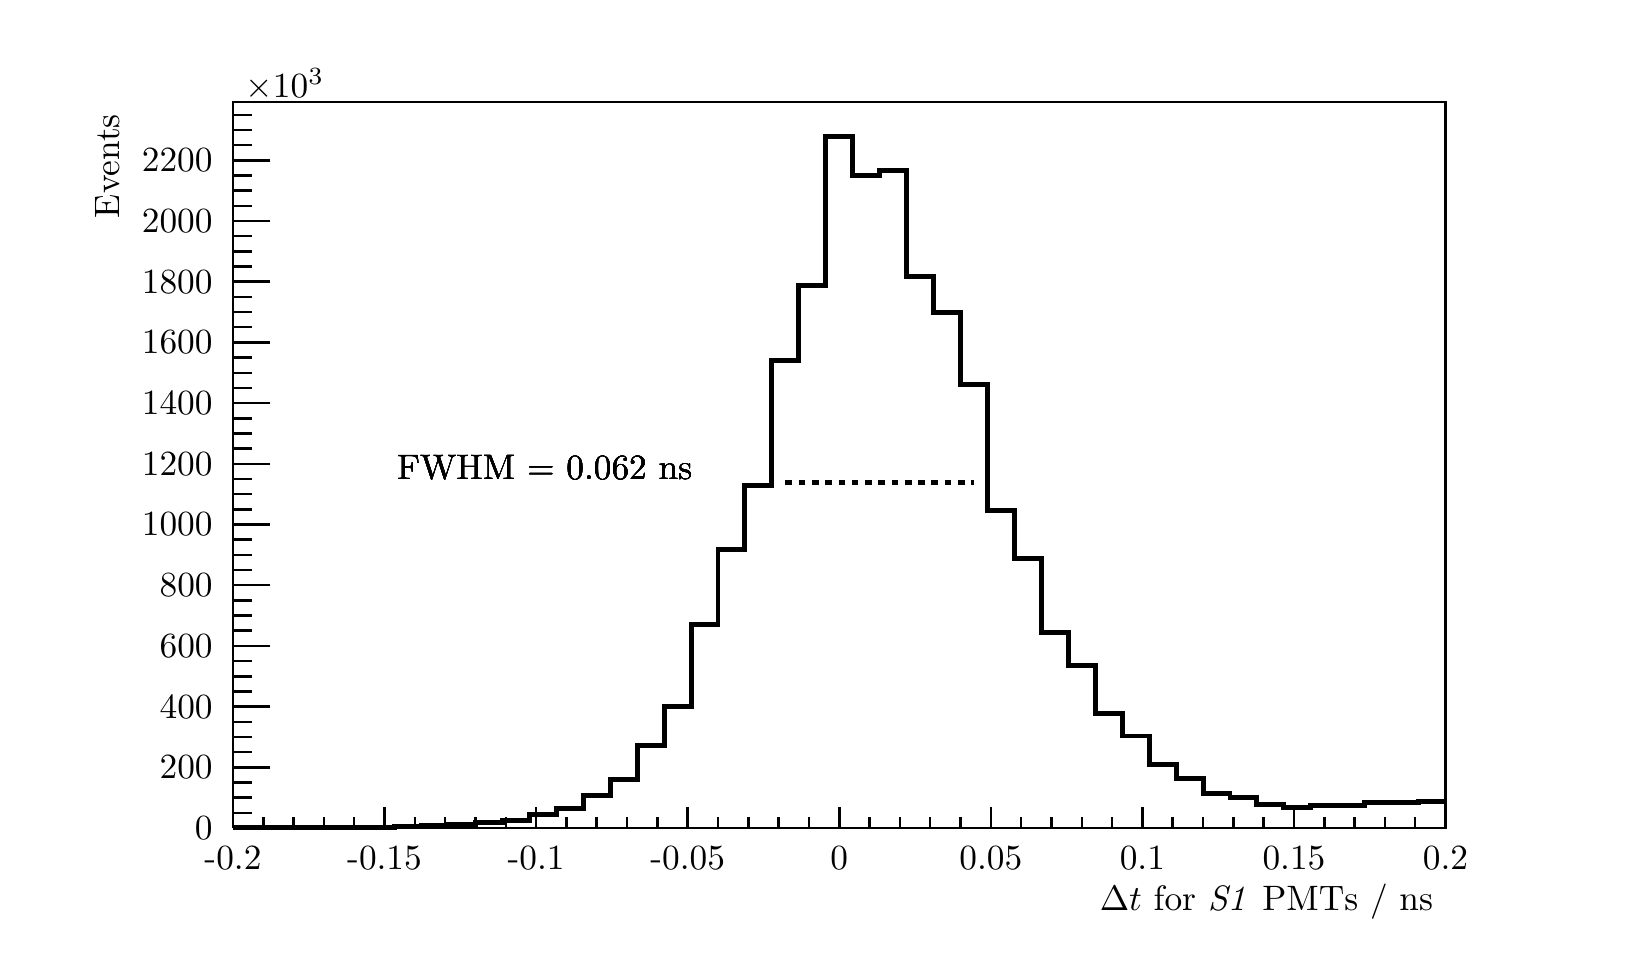
\begin{tikzpicture}
\pgfdeclareplotmark{cross} {
\pgfpathmoveto{\pgfpoint{-0.3\pgfplotmarksize}{\pgfplotmarksize}}
\pgfpathlineto{\pgfpoint{+0.3\pgfplotmarksize}{\pgfplotmarksize}}
\pgfpathlineto{\pgfpoint{+0.3\pgfplotmarksize}{0.3\pgfplotmarksize}}
\pgfpathlineto{\pgfpoint{+1\pgfplotmarksize}{0.3\pgfplotmarksize}}
\pgfpathlineto{\pgfpoint{+1\pgfplotmarksize}{-0.3\pgfplotmarksize}}
\pgfpathlineto{\pgfpoint{+0.3\pgfplotmarksize}{-0.3\pgfplotmarksize}}
\pgfpathlineto{\pgfpoint{+0.3\pgfplotmarksize}{-1.\pgfplotmarksize}}
\pgfpathlineto{\pgfpoint{-0.3\pgfplotmarksize}{-1.\pgfplotmarksize}}
\pgfpathlineto{\pgfpoint{-0.3\pgfplotmarksize}{-0.3\pgfplotmarksize}}
\pgfpathlineto{\pgfpoint{-1.\pgfplotmarksize}{-0.3\pgfplotmarksize}}
\pgfpathlineto{\pgfpoint{-1.\pgfplotmarksize}{0.3\pgfplotmarksize}}
\pgfpathlineto{\pgfpoint{-0.3\pgfplotmarksize}{0.3\pgfplotmarksize}}
\pgfpathclose
\pgfusepathqstroke
}
\pgfdeclareplotmark{cross*} {
\pgfpathmoveto{\pgfpoint{-0.3\pgfplotmarksize}{\pgfplotmarksize}}
\pgfpathlineto{\pgfpoint{+0.3\pgfplotmarksize}{\pgfplotmarksize}}
\pgfpathlineto{\pgfpoint{+0.3\pgfplotmarksize}{0.3\pgfplotmarksize}}
\pgfpathlineto{\pgfpoint{+1\pgfplotmarksize}{0.3\pgfplotmarksize}}
\pgfpathlineto{\pgfpoint{+1\pgfplotmarksize}{-0.3\pgfplotmarksize}}
\pgfpathlineto{\pgfpoint{+0.3\pgfplotmarksize}{-0.3\pgfplotmarksize}}
\pgfpathlineto{\pgfpoint{+0.3\pgfplotmarksize}{-1.\pgfplotmarksize}}
\pgfpathlineto{\pgfpoint{-0.3\pgfplotmarksize}{-1.\pgfplotmarksize}}
\pgfpathlineto{\pgfpoint{-0.3\pgfplotmarksize}{-0.3\pgfplotmarksize}}
\pgfpathlineto{\pgfpoint{-1.\pgfplotmarksize}{-0.3\pgfplotmarksize}}
\pgfpathlineto{\pgfpoint{-1.\pgfplotmarksize}{0.3\pgfplotmarksize}}
\pgfpathlineto{\pgfpoint{-0.3\pgfplotmarksize}{0.3\pgfplotmarksize}}
\pgfpathclose
\pgfusepathqfillstroke
}
\pgfdeclareplotmark{newstar} {
\pgfpathmoveto{\pgfqpoint{0pt}{\pgfplotmarksize}}
\pgfpathlineto{\pgfqpointpolar{44}{0.5\pgfplotmarksize}}
\pgfpathlineto{\pgfqpointpolar{18}{\pgfplotmarksize}}
\pgfpathlineto{\pgfqpointpolar{-20}{0.5\pgfplotmarksize}}
\pgfpathlineto{\pgfqpointpolar{-54}{\pgfplotmarksize}}
\pgfpathlineto{\pgfqpointpolar{-90}{0.5\pgfplotmarksize}}
\pgfpathlineto{\pgfqpointpolar{234}{\pgfplotmarksize}}
\pgfpathlineto{\pgfqpointpolar{198}{0.5\pgfplotmarksize}}
\pgfpathlineto{\pgfqpointpolar{162}{\pgfplotmarksize}}
\pgfpathlineto{\pgfqpointpolar{134}{0.5\pgfplotmarksize}}
\pgfpathclose
\pgfusepathqstroke
}
\pgfdeclareplotmark{newstar*} {
\pgfpathmoveto{\pgfqpoint{0pt}{\pgfplotmarksize}}
\pgfpathlineto{\pgfqpointpolar{44}{0.5\pgfplotmarksize}}
\pgfpathlineto{\pgfqpointpolar{18}{\pgfplotmarksize}}
\pgfpathlineto{\pgfqpointpolar{-20}{0.5\pgfplotmarksize}}
\pgfpathlineto{\pgfqpointpolar{-54}{\pgfplotmarksize}}
\pgfpathlineto{\pgfqpointpolar{-90}{0.5\pgfplotmarksize}}
\pgfpathlineto{\pgfqpointpolar{234}{\pgfplotmarksize}}
\pgfpathlineto{\pgfqpointpolar{198}{0.5\pgfplotmarksize}}
\pgfpathlineto{\pgfqpointpolar{162}{\pgfplotmarksize}}
\pgfpathlineto{\pgfqpointpolar{134}{0.5\pgfplotmarksize}}
\pgfpathclose
\pgfusepathqfillstroke
}
\definecolor{c}{rgb}{1,1,1};
\draw [color=c, fill=c] (0,0) rectangle (20,11.675);
\draw [color=c, fill=c] (2.6,1.51775) rectangle (18,10.741);
\definecolor{c}{rgb}{0,0,0};
\draw [c,line width=0.9] (2.6,1.51775) -- (2.6,10.741) -- (18,10.741) -- (18,1.51775) -- (2.6,1.51775);
\definecolor{c}{rgb}{1,1,1};
\draw [color=c, fill=c] (2.6,1.51775) rectangle (18,10.741);
\definecolor{c}{rgb}{0,0,0};
\draw [c,line width=0.9] (2.6,1.51775) -- (2.6,10.741) -- (18,10.741) -- (18,1.51775) -- (2.6,1.51775);
\draw [c,line width=1.8] (2.6,1.51958) -- (2.94222,1.51958) -- (2.94222,1.51977) -- (3.28444,1.51977) -- (3.28444,1.52075) -- (3.62667,1.52075) -- (3.62667,1.52204) -- (3.96889,1.52204) -- (3.96889,1.52504) -- (4.31111,1.52504) -- (4.31111,1.52834)
 -- (4.65333,1.52834) -- (4.65333,1.53523) -- (4.99556,1.53523) -- (4.99556,1.54741) -- (5.33778,1.54741) -- (5.33778,1.5584) -- (5.68,1.5584) -- (5.68,1.58483) -- (6.02222,1.58483) -- (6.02222,1.61641) -- (6.36444,1.61641) -- (6.36444,1.68501) --
 (6.70667,1.68501) -- (6.70667,1.76425) -- (7.04889,1.76425) -- (7.04889,1.93053) -- (7.39111,1.93053) -- (7.39111,2.12776) -- (7.73333,2.12776) -- (7.73333,2.57125) -- (8.07556,2.57125) -- (8.07556,3.05548) -- (8.41778,3.05548) -- (8.41778,4.09746)
 -- (8.76,4.09746) -- (8.76,5.05002) -- (9.10222,5.05002) -- (9.10222,5.87277) -- (9.44444,5.87277) -- (9.44444,7.45651) -- (9.78667,7.45651) -- (9.78667,8.4135) -- (10.1289,8.4135) -- (10.1289,10.3018) -- (10.4711,10.3018) -- (10.4711,9.8074) --
 (10.8133,9.8074) -- (10.8133,9.87378) -- (11.1556,9.87378) -- (11.1556,8.52277) -- (11.4978,8.52277) -- (11.4978,8.05893) -- (11.84,8.05893) -- (11.84,7.14883) -- (12.1822,7.14883) -- (12.1822,5.55186) -- (12.5244,5.55186) -- (12.5244,4.94574) --
 (12.8667,4.94574) -- (12.8667,3.99644) -- (13.2089,3.99644) -- (13.2089,3.57792) -- (13.5511,3.57792) -- (13.5511,2.9767) -- (13.8933,2.9767) -- (13.8933,2.68633) -- (14.2356,2.68633) -- (14.2356,2.31822) -- (14.5778,2.31822) -- (14.5778,2.15102) --
 (14.92,2.15102) -- (14.92,1.96062) -- (15.2622,1.96062) -- (15.2622,1.90122) -- (15.6044,1.90122) -- (15.6044,1.81479) -- (15.9467,1.81479) -- (15.9467,1.78186) -- (16.2889,1.78186) -- (16.2889,1.80117) -- (16.6311,1.80117) -- (16.6311,1.80069) --
 (16.9733,1.80069) -- (16.9733,1.8367) -- (17.3156,1.8367) -- (17.3156,1.83646) -- (17.6578,1.83646) -- (17.6578,1.84969) -- (18,1.84969);
\draw [c,line width=0.9] (2.6,1.51775) -- (18,1.51775);
\draw [c,line width=0.9] (2.6,1.78744) -- (2.6,1.51775);
\draw [c,line width=0.9] (2.985,1.6526) -- (2.985,1.51775);
\draw [c,line width=0.9] (3.37,1.6526) -- (3.37,1.51775);
\draw [c,line width=0.9] (3.755,1.6526) -- (3.755,1.51775);
\draw [c,line width=0.9] (4.14,1.6526) -- (4.14,1.51775);
\draw [c,line width=0.9] (4.525,1.78744) -- (4.525,1.51775);
\draw [c,line width=0.9] (4.91,1.6526) -- (4.91,1.51775);
\draw [c,line width=0.9] (5.295,1.6526) -- (5.295,1.51775);
\draw [c,line width=0.9] (5.68,1.6526) -- (5.68,1.51775);
\draw [c,line width=0.9] (6.065,1.6526) -- (6.065,1.51775);
\draw [c,line width=0.9] (6.45,1.78744) -- (6.45,1.51775);
\draw [c,line width=0.9] (6.835,1.6526) -- (6.835,1.51775);
\draw [c,line width=0.9] (7.22,1.6526) -- (7.22,1.51775);
\draw [c,line width=0.9] (7.605,1.6526) -- (7.605,1.51775);
\draw [c,line width=0.9] (7.99,1.6526) -- (7.99,1.51775);
\draw [c,line width=0.9] (8.375,1.78744) -- (8.375,1.51775);
\draw [c,line width=0.9] (8.76,1.6526) -- (8.76,1.51775);
\draw [c,line width=0.9] (9.145,1.6526) -- (9.145,1.51775);
\draw [c,line width=0.9] (9.53,1.6526) -- (9.53,1.51775);
\draw [c,line width=0.9] (9.915,1.6526) -- (9.915,1.51775);
\draw [c,line width=0.9] (10.3,1.78744) -- (10.3,1.51775);
\draw [c,line width=0.9] (10.685,1.6526) -- (10.685,1.51775);
\draw [c,line width=0.9] (11.07,1.6526) -- (11.07,1.51775);
\draw [c,line width=0.9] (11.455,1.6526) -- (11.455,1.51775);
\draw [c,line width=0.9] (11.84,1.6526) -- (11.84,1.51775);
\draw [c,line width=0.9] (12.225,1.78744) -- (12.225,1.51775);
\draw [c,line width=0.9] (12.61,1.6526) -- (12.61,1.51775);
\draw [c,line width=0.9] (12.995,1.6526) -- (12.995,1.51775);
\draw [c,line width=0.9] (13.38,1.6526) -- (13.38,1.51775);
\draw [c,line width=0.9] (13.765,1.6526) -- (13.765,1.51775);
\draw [c,line width=0.9] (14.15,1.78744) -- (14.15,1.51775);
\draw [c,line width=0.9] (14.535,1.6526) -- (14.535,1.51775);
\draw [c,line width=0.9] (14.92,1.6526) -- (14.92,1.51775);
\draw [c,line width=0.9] (15.305,1.6526) -- (15.305,1.51775);
\draw [c,line width=0.9] (15.69,1.6526) -- (15.69,1.51775);
\draw [c,line width=0.9] (16.075,1.78744) -- (16.075,1.51775);
\draw [c,line width=0.9] (16.46,1.6526) -- (16.46,1.51775);
\draw [c,line width=0.9] (16.845,1.6526) -- (16.845,1.51775);
\draw [c,line width=0.9] (17.23,1.6526) -- (17.23,1.51775);
\draw [c,line width=0.9] (17.615,1.6526) -- (17.615,1.51775);
\draw [c,line width=0.9] (18,1.78744) -- (18,1.51775);
\draw [anchor=base] (2.6,0.992375) node[scale=1.27706, color=c, rotate=0]{-0.2};
\draw [anchor=base] (4.525,0.992375) node[scale=1.27706, color=c, rotate=0]{-0.15};
\draw [anchor=base] (6.45,0.992375) node[scale=1.27706, color=c, rotate=0]{-0.1};
\draw [anchor=base] (8.375,0.992375) node[scale=1.27706, color=c, rotate=0]{-0.05};
\draw [anchor=base] (10.3,0.992375) node[scale=1.27706, color=c, rotate=0]{0};
\draw [anchor=base] (12.225,0.992375) node[scale=1.27706, color=c, rotate=0]{0.05};
\draw [anchor=base] (14.15,0.992375) node[scale=1.27706, color=c, rotate=0]{0.1};
\draw [anchor=base] (16.075,0.992375) node[scale=1.27706, color=c, rotate=0]{0.15};
\draw [anchor=base] (18,0.992375) node[scale=1.27706, color=c, rotate=0]{0.2};
\draw [anchor= east] (18,0.58375) node[scale=1.27706, color=c, rotate=0]{$\Delta t$ for $\mathit{S1}$ PMTs / ns};
\draw [c,line width=0.9] (2.6,1.51775) -- (2.6,10.741);
\draw [c,line width=0.9] (3.074,1.51775) -- (2.6,1.51775);
\draw [c,line width=0.9] (2.837,1.71046) -- (2.6,1.71046);
\draw [c,line width=0.9] (2.837,1.90318) -- (2.6,1.90318);
\draw [c,line width=0.9] (2.837,2.09589) -- (2.6,2.09589);
\draw [c,line width=0.9] (3.074,2.2886) -- (2.6,2.2886);
\draw [c,line width=0.9] (2.837,2.48132) -- (2.6,2.48132);
\draw [c,line width=0.9] (2.837,2.67403) -- (2.6,2.67403);
\draw [c,line width=0.9] (2.837,2.86674) -- (2.6,2.86674);
\draw [c,line width=0.9] (3.074,3.05946) -- (2.6,3.05946);
\draw [c,line width=0.9] (2.837,3.25217) -- (2.6,3.25217);
\draw [c,line width=0.9] (2.837,3.44488) -- (2.6,3.44488);
\draw [c,line width=0.9] (2.837,3.6376) -- (2.6,3.6376);
\draw [c,line width=0.9] (3.074,3.83031) -- (2.6,3.83031);
\draw [c,line width=0.9] (2.837,4.02302) -- (2.6,4.02302);
\draw [c,line width=0.9] (2.837,4.21574) -- (2.6,4.21574);
\draw [c,line width=0.9] (2.837,4.40845) -- (2.6,4.40845);
\draw [c,line width=0.9] (3.074,4.60116) -- (2.6,4.60116);
\draw [c,line width=0.9] (2.837,4.79388) -- (2.6,4.79388);
\draw [c,line width=0.9] (2.837,4.98659) -- (2.6,4.98659);
\draw [c,line width=0.9] (2.837,5.1793) -- (2.6,5.1793);
\draw [c,line width=0.9] (3.074,5.37202) -- (2.6,5.37202);
\draw [c,line width=0.9] (2.837,5.56473) -- (2.6,5.56473);
\draw [c,line width=0.9] (2.837,5.75744) -- (2.6,5.75744);
\draw [c,line width=0.9] (2.837,5.95016) -- (2.6,5.95016);
\draw [c,line width=0.9] (3.074,6.14287) -- (2.6,6.14287);
\draw [c,line width=0.9] (2.837,6.33558) -- (2.6,6.33558);
\draw [c,line width=0.9] (2.837,6.5283) -- (2.6,6.5283);
\draw [c,line width=0.9] (2.837,6.72101) -- (2.6,6.72101);
\draw [c,line width=0.9] (3.074,6.91372) -- (2.6,6.91372);
\draw [c,line width=0.9] (2.837,7.10644) -- (2.6,7.10644);
\draw [c,line width=0.9] (2.837,7.29915) -- (2.6,7.29915);
\draw [c,line width=0.9] (2.837,7.49186) -- (2.6,7.49186);
\draw [c,line width=0.9] (3.074,7.68458) -- (2.6,7.68458);
\draw [c,line width=0.9] (2.837,7.87729) -- (2.6,7.87729);
\draw [c,line width=0.9] (2.837,8.07) -- (2.6,8.07);
\draw [c,line width=0.9] (2.837,8.26272) -- (2.6,8.26272);
\draw [c,line width=0.9] (3.074,8.45543) -- (2.6,8.45543);
\draw [c,line width=0.9] (2.837,8.64814) -- (2.6,8.64814);
\draw [c,line width=0.9] (2.837,8.84086) -- (2.6,8.84086);
\draw [c,line width=0.9] (2.837,9.03357) -- (2.6,9.03357);
\draw [c,line width=0.9] (3.074,9.22628) -- (2.6,9.22628);
\draw [c,line width=0.9] (2.837,9.419) -- (2.6,9.419);
\draw [c,line width=0.9] (2.837,9.61171) -- (2.6,9.61171);
\draw [c,line width=0.9] (2.837,9.80442) -- (2.6,9.80442);
\draw [c,line width=0.9] (3.074,9.99714) -- (2.6,9.99714);
\draw [c,line width=0.9] (3.074,9.99714) -- (2.6,9.99714);
\draw [c,line width=0.9] (2.837,10.1899) -- (2.6,10.1899);
\draw [c,line width=0.9] (2.837,10.3826) -- (2.6,10.3826);
\draw [c,line width=0.9] (2.837,10.5753) -- (2.6,10.5753);
\draw [anchor= east] (2.5,1.51775) node[scale=1.27706, color=c, rotate=0]{0};
\draw [anchor= east] (2.5,2.2886) node[scale=1.27706, color=c, rotate=0]{200};
\draw [anchor= east] (2.5,3.05946) node[scale=1.27706, color=c, rotate=0]{400};
\draw [anchor= east] (2.5,3.83031) node[scale=1.27706, color=c, rotate=0]{600};
\draw [anchor= east] (2.5,4.60116) node[scale=1.27706, color=c, rotate=0]{800};
\draw [anchor= east] (2.5,5.37202) node[scale=1.27706, color=c, rotate=0]{1000};
\draw [anchor= east] (2.5,6.14287) node[scale=1.27706, color=c, rotate=0]{1200};
\draw [anchor= east] (2.5,6.91372) node[scale=1.27706, color=c, rotate=0]{1400};
\draw [anchor= east] (2.5,7.68458) node[scale=1.27706, color=c, rotate=0]{1600};
\draw [anchor= east] (2.5,8.45543) node[scale=1.27706, color=c, rotate=0]{1800};
\draw [anchor= east] (2.5,9.22628) node[scale=1.27706, color=c, rotate=0]{2000};
\draw [anchor= east] (2.5,9.99714) node[scale=1.27706, color=c, rotate=0]{2200};
\draw [anchor=base west] (2.6,10.7994) node[scale=1.27706, color=c, rotate=0]{$\times10^{3}$};
\draw [anchor= east] (1,10.741) node[scale=1.27706, color=c, rotate=90]{ Events};
\draw [c,dash pattern=on 2.40pt off 2.40pt ,line width=1.8] (9.61556,5.90977) -- (12.0111,5.90977);
\draw [anchor=base west] (4.525,5.95016) node[scale=1.27706, color=c, rotate=0]{FWHM = 0.062 ns};
\draw [anchor=base west] (4.525,5.95016) node[scale=1.27706, color=c, rotate=0]{FWHM = 0.062 ns};
\draw [anchor=base west] (4.525,5.95016) node[scale=1.27706, color=c, rotate=0]{FWHM = 0.062 ns};
\draw [anchor=base west] (4.525,5.95016) node[scale=1.27706, color=c, rotate=0]{FWHM = 0.062 ns};
\draw [anchor=base west] (4.525,5.95016) node[scale=1.27706, color=c, rotate=0]{FWHM = 0.062 ns};
\end{tikzpicture}

  \end{adjustbox}
  \caption{An example of the timing spread of $\mathit{S1}$ hits. The time is calculated as an average of the hit time as measured in each of the four PMTs.}
  \label{fig:s1Res}
\end{figure}

The $\mathit{S2}$ counter is a scintillator tile of size $120\times120\times5$~mm$^3$, coupled to a 2" Hamamatsu Photonics R1309 PMT~\cite{Hamamatsu}, via a long light-guide as shown in Figure~\ref{fig:modblocks}.
The $\mathit{S2}$ counter was placed $(1.419 \pm 0.001)~\text{m}$ downstream of $\mathit{S1}$.
The transverse position of $\mathit{S2}$ was adjusted to account for the beam divergence in the moderator blocks.

The analog signals from one of the $\mathit{S1}$ PMTs and the $\mathit{S2}$ PMT were fed into LeCroy 620AL NIM discriminator units with a threshold of 30~mV.
Subsequently, the discriminated signals were fed into a NIM coincidence unit, whose output was recorded by the DAQ systems of the downstream ToF ($\mathit{S4}$) wall.
This information was further used for the time-of-flight analysis of $\mathit{S4}$.

\subsection{Upstream Time of Flight instrumentation (S3)}
\label{subsec:s3Exp}
The $\mathit{S3}$ `upstream' ToF constituent was placed $(1.323 \pm 0.001)~\text{m}$ upstream of the upstream side of the HPTPC drift volume in the beamline.
A schematic drawing of the $\mathit{S3}$ ToF wall is shown in Figure~\ref{fig:S3sketch}.
The detector comprises 22 staggered scintillator bars:  20 bars with dimensions $168 \times 6.0 \times 1.0$~cm$^3$ and 2 bars of  $150 \times 6.0 \times 1.0$~cm$^3$ placed on top and bottom~\cite{S3-proceedings}.
The overlap between bars was set to 5~mm, thus the active area of the detector was $2.0214~\text{cm}^{2}$.

\begin{figure}
  \centering
  \includegraphics[width=0.54\linewidth]{files/Figures/uToF_sketch.pdf}
  \hfill
  \includegraphics[width=0.43\linewidth]{files/Figures/uTOF_rot.pdf}
  \caption{Sketch of the $\mathit{S3}$ wall \cite{S3-proceedings}.
  Front (left) and rotated (right) views are presented.}
  \label{fig:S3sketch}
\end{figure}

The bars are made from EJ-200~\cite{SCIONIX} plastic scintillator, which provides a brightness of 10,000~photons/MeV~deposited.
It also has a suitable optical attenuation length of 4~m and fast timing, with a rise time of 0.9~ns and decay time constant of 2.1~ns.
The scintillation emission spectrum of EJ-200 peaks in the violet region of the visible spectrum (435~nm)~\cite{EJ200}.
The bars were wrapped in an aluminium foil (60\% reflectivity) to increase the collected light.

Arrays of eight $6 \times 6$~mm$^2$ area silicon photomultipliers (SiPMs) S13360-6050PE from Hamamatsu Photonics \cite{Hamamatsu} were coupled to each end of the bar to collect scintillation photons.
The photon detection efficiency at the peak sensitivity wavelength (450~nm) is 40\%~\cite{Hamamatsu}.
The anode signals of the SiPMs are read out, summed and shaped by a dedicated circuit as described in Ref.\,\cite{S3-readout}.
%an 8-channel SiPM anode readout integrated circuit MUSIC-R1. %The construction of the prototype was a joint effort between groups of Geneva and Zurich universities as a part of R\&D for the Timing detector of the SHIP experiment \cite{AK}.

$\mathit{S3}$ uses a 64 channel data acquisition system based on the SAMPIC chip.
A SAMPIC chip is a waveform and time to digital converter (WTDC) 16-channel ASIC which provides a raw time with ultrafast analog memory allowing fine timing extraction as well as other parameters of the pulse~\cite{SAMPIC}.
Each channel contains a discriminator that can trigger itself independently or participate in a more complex combined trigger. 
Three ASIC modules ($16\times3=48$ channels) were connected to the 44 channels of $\mathit{S3}$ and were operated in self-triggering mode.

The trigger conditions are as follows. At least three out of the four $\mathit{S1}$ PMTs must have a signal above a 30~mV threshold.
Additionally, there must be at least one signal in $\mathit{S3}$ above 30~mV.
These $\mathit{S1}$ and $\mathit{S3}$ signals must be coincident within a gate of 70~ns.
A fourth ASIC was used to acquire data from $\mathit{S1}$, the coincidence signal $\mathit{S1} \cap \mathit{S2}$, and the start-of-spill signal from the PS.
%A second level trigger was implemented in firmware and run on the level of the ASICs: the data were only sent to the hard disk of the DAQ computer if there was a coincidence between the $\mathit{S1}$ channels and at least one of the channels in the ASICs used for $\mathit{S3}$.
The mean time of light signals detected at both ends of a single bar provides a time reference with a resolution of about 100~ps, while the difference between the time of the light signals gives the position of the interaction along the bar, with a resolution of 1.6~cm.

Examples of reconstructed $\mathit{S3}$ spatial distributions are shown in Figure~\ref{fig:s3XY_pion}.
Figure~\ref{fig:s3XY_pion}, left, shows the spatial distribution of hits in $\mathit{S3}$ thought to be produced by MIPs when no moderator was present in the beamline.
Figure~\ref{fig:s3XY_pion}, right, shows the spatial distribution of hits identified in $\mathit{S3}$ as protons when 4 moderator blocks were in the beamline.
The pattern of hits is more diffuse, illustrating the scattering effect of the moderator blocks.
When in this position the measured horizontal FWHM of the unmoderated beam is 16.8~cm while the vertical FWHM is 11.0~cm.

\begin{figure}[t]
  \begin{minipage}[t]{0.49\textwidth}
    \centering
    \begin{adjustbox}{max totalsize={\textwidth}{.5\textheight},center}
      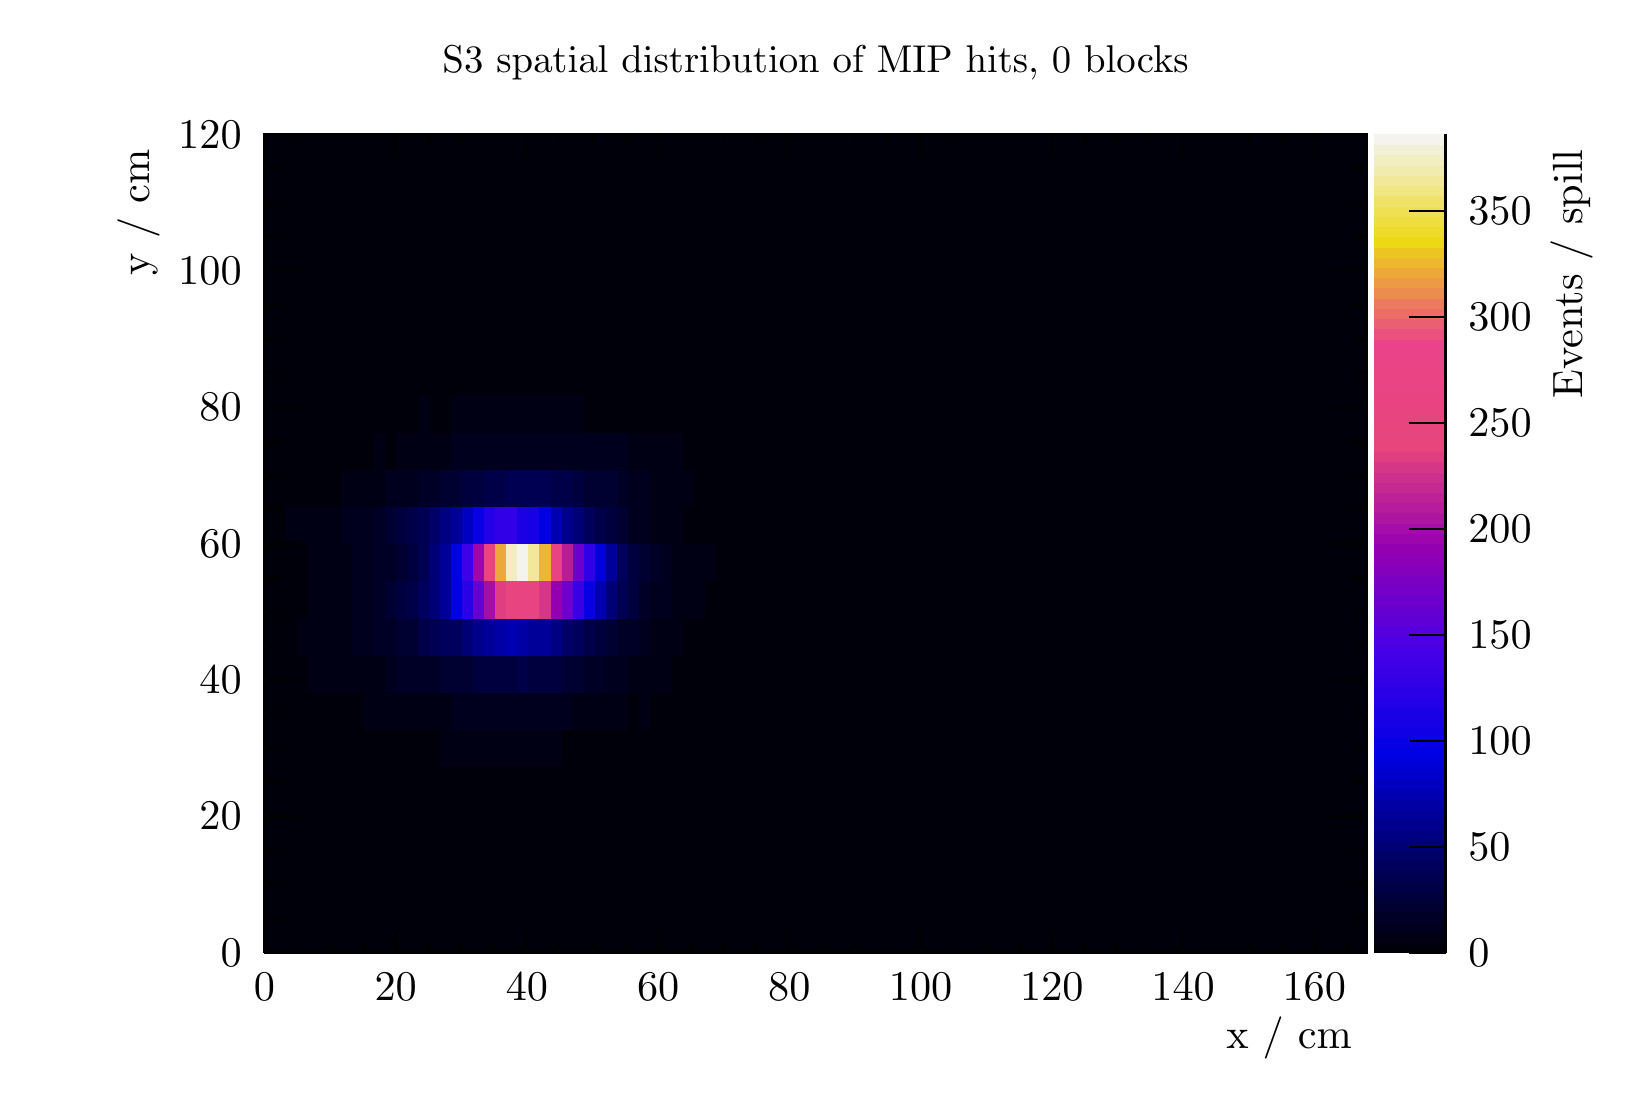
\begin{tikzpicture}
\pgfdeclareplotmark{cross} {
\pgfpathmoveto{\pgfpoint{-0.3\pgfplotmarksize}{\pgfplotmarksize}}
\pgfpathlineto{\pgfpoint{+0.3\pgfplotmarksize}{\pgfplotmarksize}}
\pgfpathlineto{\pgfpoint{+0.3\pgfplotmarksize}{0.3\pgfplotmarksize}}
\pgfpathlineto{\pgfpoint{+1\pgfplotmarksize}{0.3\pgfplotmarksize}}
\pgfpathlineto{\pgfpoint{+1\pgfplotmarksize}{-0.3\pgfplotmarksize}}
\pgfpathlineto{\pgfpoint{+0.3\pgfplotmarksize}{-0.3\pgfplotmarksize}}
\pgfpathlineto{\pgfpoint{+0.3\pgfplotmarksize}{-1.\pgfplotmarksize}}
\pgfpathlineto{\pgfpoint{-0.3\pgfplotmarksize}{-1.\pgfplotmarksize}}
\pgfpathlineto{\pgfpoint{-0.3\pgfplotmarksize}{-0.3\pgfplotmarksize}}
\pgfpathlineto{\pgfpoint{-1.\pgfplotmarksize}{-0.3\pgfplotmarksize}}
\pgfpathlineto{\pgfpoint{-1.\pgfplotmarksize}{0.3\pgfplotmarksize}}
\pgfpathlineto{\pgfpoint{-0.3\pgfplotmarksize}{0.3\pgfplotmarksize}}
\pgfpathclose
\pgfusepathqstroke
}
\pgfdeclareplotmark{cross*} {
\pgfpathmoveto{\pgfpoint{-0.3\pgfplotmarksize}{\pgfplotmarksize}}
\pgfpathlineto{\pgfpoint{+0.3\pgfplotmarksize}{\pgfplotmarksize}}
\pgfpathlineto{\pgfpoint{+0.3\pgfplotmarksize}{0.3\pgfplotmarksize}}
\pgfpathlineto{\pgfpoint{+1\pgfplotmarksize}{0.3\pgfplotmarksize}}
\pgfpathlineto{\pgfpoint{+1\pgfplotmarksize}{-0.3\pgfplotmarksize}}
\pgfpathlineto{\pgfpoint{+0.3\pgfplotmarksize}{-0.3\pgfplotmarksize}}
\pgfpathlineto{\pgfpoint{+0.3\pgfplotmarksize}{-1.\pgfplotmarksize}}
\pgfpathlineto{\pgfpoint{-0.3\pgfplotmarksize}{-1.\pgfplotmarksize}}
\pgfpathlineto{\pgfpoint{-0.3\pgfplotmarksize}{-0.3\pgfplotmarksize}}
\pgfpathlineto{\pgfpoint{-1.\pgfplotmarksize}{-0.3\pgfplotmarksize}}
\pgfpathlineto{\pgfpoint{-1.\pgfplotmarksize}{0.3\pgfplotmarksize}}
\pgfpathlineto{\pgfpoint{-0.3\pgfplotmarksize}{0.3\pgfplotmarksize}}
\pgfpathclose
\pgfusepathqfillstroke
}
\pgfdeclareplotmark{newstar} {
\pgfpathmoveto{\pgfqpoint{0pt}{\pgfplotmarksize}}
\pgfpathlineto{\pgfqpointpolar{44}{0.5\pgfplotmarksize}}
\pgfpathlineto{\pgfqpointpolar{18}{\pgfplotmarksize}}
\pgfpathlineto{\pgfqpointpolar{-20}{0.5\pgfplotmarksize}}
\pgfpathlineto{\pgfqpointpolar{-54}{\pgfplotmarksize}}
\pgfpathlineto{\pgfqpointpolar{-90}{0.5\pgfplotmarksize}}
\pgfpathlineto{\pgfqpointpolar{234}{\pgfplotmarksize}}
\pgfpathlineto{\pgfqpointpolar{198}{0.5\pgfplotmarksize}}
\pgfpathlineto{\pgfqpointpolar{162}{\pgfplotmarksize}}
\pgfpathlineto{\pgfqpointpolar{134}{0.5\pgfplotmarksize}}
\pgfpathclose
\pgfusepathqstroke
}
\pgfdeclareplotmark{newstar*} {
\pgfpathmoveto{\pgfqpoint{0pt}{\pgfplotmarksize}}
\pgfpathlineto{\pgfqpointpolar{44}{0.5\pgfplotmarksize}}
\pgfpathlineto{\pgfqpointpolar{18}{\pgfplotmarksize}}
\pgfpathlineto{\pgfqpointpolar{-20}{0.5\pgfplotmarksize}}
\pgfpathlineto{\pgfqpointpolar{-54}{\pgfplotmarksize}}
\pgfpathlineto{\pgfqpointpolar{-90}{0.5\pgfplotmarksize}}
\pgfpathlineto{\pgfqpointpolar{234}{\pgfplotmarksize}}
\pgfpathlineto{\pgfqpointpolar{198}{0.5\pgfplotmarksize}}
\pgfpathlineto{\pgfqpointpolar{162}{\pgfplotmarksize}}
\pgfpathlineto{\pgfqpointpolar{134}{0.5\pgfplotmarksize}}
\pgfpathclose
\pgfusepathqfillstroke
}
\definecolor{c}{rgb}{1,1,1};
\draw [color=c, fill=c] (0,0) rectangle (20,13.4957);
\draw [color=c, fill=c] (3,1.75444) rectangle (17,12.1461);
\definecolor{c}{rgb}{0,0,0};
\draw [c,line width=0.9] (3,1.75444) -- (3,12.1461) -- (17,12.1461) -- (17,1.75444) -- (3,1.75444);
\definecolor{c}{rgb}{1,1,1};
\draw [color=c, fill=c] (3,1.75444) rectangle (17,12.1461);
\definecolor{c}{rgb}{0,0,0};
\draw [c,line width=0.9] (3,1.75444) -- (3,12.1461) -- (17,12.1461) -- (17,1.75444) -- (3,1.75444);
\definecolor{c}{rgb}{0,0,0.0387097};
\draw [color=c, fill=c] (3,1.75444) rectangle (3.14,2.22679);
\draw [color=c, fill=c] (3.14,1.75444) rectangle (3.28,2.22679);
\draw [color=c, fill=c] (3.28,1.75444) rectangle (3.42,2.22679);
\draw [color=c, fill=c] (3.42,1.75444) rectangle (3.56,2.22679);
\draw [color=c, fill=c] (3.56,1.75444) rectangle (3.7,2.22679);
\draw [color=c, fill=c] (3.7,1.75444) rectangle (3.84,2.22679);
\draw [color=c, fill=c] (3.84,1.75444) rectangle (3.98,2.22679);
\draw [color=c, fill=c] (3.98,1.75444) rectangle (4.12,2.22679);
\draw [color=c, fill=c] (4.12,1.75444) rectangle (4.26,2.22679);
\draw [color=c, fill=c] (4.26,1.75444) rectangle (4.4,2.22679);
\draw [color=c, fill=c] (4.4,1.75444) rectangle (4.54,2.22679);
\draw [color=c, fill=c] (4.54,1.75444) rectangle (4.68,2.22679);
\draw [color=c, fill=c] (4.68,1.75444) rectangle (4.82,2.22679);
\draw [color=c, fill=c] (4.82,1.75444) rectangle (4.96,2.22679);
\draw [color=c, fill=c] (4.96,1.75444) rectangle (5.1,2.22679);
\draw [color=c, fill=c] (5.1,1.75444) rectangle (5.24,2.22679);
\draw [color=c, fill=c] (5.24,1.75444) rectangle (5.38,2.22679);
\draw [color=c, fill=c] (5.38,1.75444) rectangle (5.52,2.22679);
\draw [color=c, fill=c] (5.52,1.75444) rectangle (5.66,2.22679);
\draw [color=c, fill=c] (5.66,1.75444) rectangle (5.8,2.22679);
\draw [color=c, fill=c] (5.8,1.75444) rectangle (5.94,2.22679);
\draw [color=c, fill=c] (5.94,1.75444) rectangle (6.08,2.22679);
\draw [color=c, fill=c] (6.08,1.75444) rectangle (6.22,2.22679);
\draw [color=c, fill=c] (6.22,1.75444) rectangle (6.36,2.22679);
\draw [color=c, fill=c] (6.36,1.75444) rectangle (6.5,2.22679);
\draw [color=c, fill=c] (6.5,1.75444) rectangle (6.64,2.22679);
\draw [color=c, fill=c] (6.64,1.75444) rectangle (6.78,2.22679);
\draw [color=c, fill=c] (6.78,1.75444) rectangle (6.92,2.22679);
\draw [color=c, fill=c] (6.92,1.75444) rectangle (7.06,2.22679);
\draw [color=c, fill=c] (7.06,1.75444) rectangle (7.2,2.22679);
\draw [color=c, fill=c] (7.2,1.75444) rectangle (7.34,2.22679);
\draw [color=c, fill=c] (7.34,1.75444) rectangle (7.48,2.22679);
\draw [color=c, fill=c] (7.48,1.75444) rectangle (7.62,2.22679);
\draw [color=c, fill=c] (7.62,1.75444) rectangle (7.76,2.22679);
\draw [color=c, fill=c] (7.76,1.75444) rectangle (7.9,2.22679);
\draw [color=c, fill=c] (7.9,1.75444) rectangle (8.04,2.22679);
\draw [color=c, fill=c] (8.04,1.75444) rectangle (8.18,2.22679);
\draw [color=c, fill=c] (8.18,1.75444) rectangle (8.32,2.22679);
\draw [color=c, fill=c] (8.32,1.75444) rectangle (8.46,2.22679);
\draw [color=c, fill=c] (8.46,1.75444) rectangle (8.6,2.22679);
\draw [color=c, fill=c] (8.6,1.75444) rectangle (8.74,2.22679);
\draw [color=c, fill=c] (8.74,1.75444) rectangle (8.88,2.22679);
\draw [color=c, fill=c] (8.88,1.75444) rectangle (9.02,2.22679);
\draw [color=c, fill=c] (9.02,1.75444) rectangle (9.16,2.22679);
\draw [color=c, fill=c] (9.16,1.75444) rectangle (9.3,2.22679);
\draw [color=c, fill=c] (9.3,1.75444) rectangle (9.44,2.22679);
\draw [color=c, fill=c] (9.44,1.75444) rectangle (9.58,2.22679);
\draw [color=c, fill=c] (9.58,1.75444) rectangle (9.72,2.22679);
\draw [color=c, fill=c] (9.72,1.75444) rectangle (9.86,2.22679);
\draw [color=c, fill=c] (9.86,1.75444) rectangle (10,2.22679);
\draw [color=c, fill=c] (10,1.75444) rectangle (10.14,2.22679);
\draw [color=c, fill=c] (10.14,1.75444) rectangle (10.28,2.22679);
\draw [color=c, fill=c] (10.28,1.75444) rectangle (10.42,2.22679);
\draw [color=c, fill=c] (10.42,1.75444) rectangle (10.56,2.22679);
\draw [color=c, fill=c] (10.56,1.75444) rectangle (10.7,2.22679);
\draw [color=c, fill=c] (10.7,1.75444) rectangle (10.84,2.22679);
\draw [color=c, fill=c] (10.84,1.75444) rectangle (10.98,2.22679);
\draw [color=c, fill=c] (10.98,1.75444) rectangle (11.12,2.22679);
\draw [color=c, fill=c] (11.12,1.75444) rectangle (11.26,2.22679);
\draw [color=c, fill=c] (11.26,1.75444) rectangle (11.4,2.22679);
\draw [color=c, fill=c] (11.4,1.75444) rectangle (11.54,2.22679);
\draw [color=c, fill=c] (11.54,1.75444) rectangle (11.68,2.22679);
\draw [color=c, fill=c] (11.68,1.75444) rectangle (11.82,2.22679);
\draw [color=c, fill=c] (11.82,1.75444) rectangle (11.96,2.22679);
\draw [color=c, fill=c] (11.96,1.75444) rectangle (12.1,2.22679);
\draw [color=c, fill=c] (12.1,1.75444) rectangle (12.24,2.22679);
\draw [color=c, fill=c] (12.24,1.75444) rectangle (12.38,2.22679);
\draw [color=c, fill=c] (12.38,1.75444) rectangle (12.52,2.22679);
\draw [color=c, fill=c] (12.52,1.75444) rectangle (12.66,2.22679);
\draw [color=c, fill=c] (12.66,1.75444) rectangle (12.8,2.22679);
\draw [color=c, fill=c] (12.8,1.75444) rectangle (12.94,2.22679);
\draw [color=c, fill=c] (12.94,1.75444) rectangle (13.08,2.22679);
\draw [color=c, fill=c] (13.08,1.75444) rectangle (13.22,2.22679);
\draw [color=c, fill=c] (13.22,1.75444) rectangle (13.36,2.22679);
\draw [color=c, fill=c] (13.36,1.75444) rectangle (13.5,2.22679);
\draw [color=c, fill=c] (13.5,1.75444) rectangle (13.64,2.22679);
\draw [color=c, fill=c] (13.64,1.75444) rectangle (13.78,2.22679);
\draw [color=c, fill=c] (13.78,1.75444) rectangle (13.92,2.22679);
\draw [color=c, fill=c] (13.92,1.75444) rectangle (14.06,2.22679);
\draw [color=c, fill=c] (14.06,1.75444) rectangle (14.2,2.22679);
\draw [color=c, fill=c] (14.2,1.75444) rectangle (14.34,2.22679);
\draw [color=c, fill=c] (14.34,1.75444) rectangle (14.48,2.22679);
\draw [color=c, fill=c] (14.48,1.75444) rectangle (14.62,2.22679);
\draw [color=c, fill=c] (14.62,1.75444) rectangle (14.76,2.22679);
\draw [color=c, fill=c] (14.76,1.75444) rectangle (14.9,2.22679);
\draw [color=c, fill=c] (14.9,1.75444) rectangle (15.04,2.22679);
\draw [color=c, fill=c] (15.04,1.75444) rectangle (15.18,2.22679);
\draw [color=c, fill=c] (15.18,1.75444) rectangle (15.32,2.22679);
\draw [color=c, fill=c] (15.32,1.75444) rectangle (15.46,2.22679);
\draw [color=c, fill=c] (15.46,1.75444) rectangle (15.6,2.22679);
\draw [color=c, fill=c] (15.6,1.75444) rectangle (15.74,2.22679);
\draw [color=c, fill=c] (15.74,1.75444) rectangle (15.88,2.22679);
\draw [color=c, fill=c] (15.88,1.75444) rectangle (16.02,2.22679);
\draw [color=c, fill=c] (16.02,1.75444) rectangle (16.16,2.22679);
\draw [color=c, fill=c] (16.16,1.75444) rectangle (16.3,2.22679);
\draw [color=c, fill=c] (16.3,1.75444) rectangle (16.44,2.22679);
\draw [color=c, fill=c] (16.44,1.75444) rectangle (16.58,2.22679);
\draw [color=c, fill=c] (16.58,1.75444) rectangle (16.72,2.22679);
\draw [color=c, fill=c] (16.72,1.75444) rectangle (16.86,2.22679);
\draw [color=c, fill=c] (16.86,1.75444) rectangle (17,2.22679);
\draw [color=c, fill=c] (3,2.22679) rectangle (3.14,2.69914);
\draw [color=c, fill=c] (3.14,2.22679) rectangle (3.28,2.69914);
\draw [color=c, fill=c] (3.28,2.22679) rectangle (3.42,2.69914);
\draw [color=c, fill=c] (3.42,2.22679) rectangle (3.56,2.69914);
\draw [color=c, fill=c] (3.56,2.22679) rectangle (3.7,2.69914);
\draw [color=c, fill=c] (3.7,2.22679) rectangle (3.84,2.69914);
\draw [color=c, fill=c] (3.84,2.22679) rectangle (3.98,2.69914);
\draw [color=c, fill=c] (3.98,2.22679) rectangle (4.12,2.69914);
\draw [color=c, fill=c] (4.12,2.22679) rectangle (4.26,2.69914);
\draw [color=c, fill=c] (4.26,2.22679) rectangle (4.4,2.69914);
\draw [color=c, fill=c] (4.4,2.22679) rectangle (4.54,2.69914);
\draw [color=c, fill=c] (4.54,2.22679) rectangle (4.68,2.69914);
\draw [color=c, fill=c] (4.68,2.22679) rectangle (4.82,2.69914);
\draw [color=c, fill=c] (4.82,2.22679) rectangle (4.96,2.69914);
\draw [color=c, fill=c] (4.96,2.22679) rectangle (5.1,2.69914);
\draw [color=c, fill=c] (5.1,2.22679) rectangle (5.24,2.69914);
\draw [color=c, fill=c] (5.24,2.22679) rectangle (5.38,2.69914);
\draw [color=c, fill=c] (5.38,2.22679) rectangle (5.52,2.69914);
\draw [color=c, fill=c] (5.52,2.22679) rectangle (5.66,2.69914);
\draw [color=c, fill=c] (5.66,2.22679) rectangle (5.8,2.69914);
\draw [color=c, fill=c] (5.8,2.22679) rectangle (5.94,2.69914);
\draw [color=c, fill=c] (5.94,2.22679) rectangle (6.08,2.69914);
\draw [color=c, fill=c] (6.08,2.22679) rectangle (6.22,2.69914);
\draw [color=c, fill=c] (6.22,2.22679) rectangle (6.36,2.69914);
\draw [color=c, fill=c] (6.36,2.22679) rectangle (6.5,2.69914);
\draw [color=c, fill=c] (6.5,2.22679) rectangle (6.64,2.69914);
\draw [color=c, fill=c] (6.64,2.22679) rectangle (6.78,2.69914);
\draw [color=c, fill=c] (6.78,2.22679) rectangle (6.92,2.69914);
\draw [color=c, fill=c] (6.92,2.22679) rectangle (7.06,2.69914);
\draw [color=c, fill=c] (7.06,2.22679) rectangle (7.2,2.69914);
\draw [color=c, fill=c] (7.2,2.22679) rectangle (7.34,2.69914);
\draw [color=c, fill=c] (7.34,2.22679) rectangle (7.48,2.69914);
\draw [color=c, fill=c] (7.48,2.22679) rectangle (7.62,2.69914);
\draw [color=c, fill=c] (7.62,2.22679) rectangle (7.76,2.69914);
\draw [color=c, fill=c] (7.76,2.22679) rectangle (7.9,2.69914);
\draw [color=c, fill=c] (7.9,2.22679) rectangle (8.04,2.69914);
\draw [color=c, fill=c] (8.04,2.22679) rectangle (8.18,2.69914);
\draw [color=c, fill=c] (8.18,2.22679) rectangle (8.32,2.69914);
\draw [color=c, fill=c] (8.32,2.22679) rectangle (8.46,2.69914);
\draw [color=c, fill=c] (8.46,2.22679) rectangle (8.6,2.69914);
\draw [color=c, fill=c] (8.6,2.22679) rectangle (8.74,2.69914);
\draw [color=c, fill=c] (8.74,2.22679) rectangle (8.88,2.69914);
\draw [color=c, fill=c] (8.88,2.22679) rectangle (9.02,2.69914);
\draw [color=c, fill=c] (9.02,2.22679) rectangle (9.16,2.69914);
\draw [color=c, fill=c] (9.16,2.22679) rectangle (9.3,2.69914);
\draw [color=c, fill=c] (9.3,2.22679) rectangle (9.44,2.69914);
\draw [color=c, fill=c] (9.44,2.22679) rectangle (9.58,2.69914);
\draw [color=c, fill=c] (9.58,2.22679) rectangle (9.72,2.69914);
\draw [color=c, fill=c] (9.72,2.22679) rectangle (9.86,2.69914);
\draw [color=c, fill=c] (9.86,2.22679) rectangle (10,2.69914);
\draw [color=c, fill=c] (10,2.22679) rectangle (10.14,2.69914);
\draw [color=c, fill=c] (10.14,2.22679) rectangle (10.28,2.69914);
\draw [color=c, fill=c] (10.28,2.22679) rectangle (10.42,2.69914);
\draw [color=c, fill=c] (10.42,2.22679) rectangle (10.56,2.69914);
\draw [color=c, fill=c] (10.56,2.22679) rectangle (10.7,2.69914);
\draw [color=c, fill=c] (10.7,2.22679) rectangle (10.84,2.69914);
\draw [color=c, fill=c] (10.84,2.22679) rectangle (10.98,2.69914);
\draw [color=c, fill=c] (10.98,2.22679) rectangle (11.12,2.69914);
\draw [color=c, fill=c] (11.12,2.22679) rectangle (11.26,2.69914);
\draw [color=c, fill=c] (11.26,2.22679) rectangle (11.4,2.69914);
\draw [color=c, fill=c] (11.4,2.22679) rectangle (11.54,2.69914);
\draw [color=c, fill=c] (11.54,2.22679) rectangle (11.68,2.69914);
\draw [color=c, fill=c] (11.68,2.22679) rectangle (11.82,2.69914);
\draw [color=c, fill=c] (11.82,2.22679) rectangle (11.96,2.69914);
\draw [color=c, fill=c] (11.96,2.22679) rectangle (12.1,2.69914);
\draw [color=c, fill=c] (12.1,2.22679) rectangle (12.24,2.69914);
\draw [color=c, fill=c] (12.24,2.22679) rectangle (12.38,2.69914);
\draw [color=c, fill=c] (12.38,2.22679) rectangle (12.52,2.69914);
\draw [color=c, fill=c] (12.52,2.22679) rectangle (12.66,2.69914);
\draw [color=c, fill=c] (12.66,2.22679) rectangle (12.8,2.69914);
\draw [color=c, fill=c] (12.8,2.22679) rectangle (12.94,2.69914);
\draw [color=c, fill=c] (12.94,2.22679) rectangle (13.08,2.69914);
\draw [color=c, fill=c] (13.08,2.22679) rectangle (13.22,2.69914);
\draw [color=c, fill=c] (13.22,2.22679) rectangle (13.36,2.69914);
\draw [color=c, fill=c] (13.36,2.22679) rectangle (13.5,2.69914);
\draw [color=c, fill=c] (13.5,2.22679) rectangle (13.64,2.69914);
\draw [color=c, fill=c] (13.64,2.22679) rectangle (13.78,2.69914);
\draw [color=c, fill=c] (13.78,2.22679) rectangle (13.92,2.69914);
\draw [color=c, fill=c] (13.92,2.22679) rectangle (14.06,2.69914);
\draw [color=c, fill=c] (14.06,2.22679) rectangle (14.2,2.69914);
\draw [color=c, fill=c] (14.2,2.22679) rectangle (14.34,2.69914);
\draw [color=c, fill=c] (14.34,2.22679) rectangle (14.48,2.69914);
\draw [color=c, fill=c] (14.48,2.22679) rectangle (14.62,2.69914);
\draw [color=c, fill=c] (14.62,2.22679) rectangle (14.76,2.69914);
\draw [color=c, fill=c] (14.76,2.22679) rectangle (14.9,2.69914);
\draw [color=c, fill=c] (14.9,2.22679) rectangle (15.04,2.69914);
\draw [color=c, fill=c] (15.04,2.22679) rectangle (15.18,2.69914);
\draw [color=c, fill=c] (15.18,2.22679) rectangle (15.32,2.69914);
\draw [color=c, fill=c] (15.32,2.22679) rectangle (15.46,2.69914);
\draw [color=c, fill=c] (15.46,2.22679) rectangle (15.6,2.69914);
\draw [color=c, fill=c] (15.6,2.22679) rectangle (15.74,2.69914);
\draw [color=c, fill=c] (15.74,2.22679) rectangle (15.88,2.69914);
\draw [color=c, fill=c] (15.88,2.22679) rectangle (16.02,2.69914);
\draw [color=c, fill=c] (16.02,2.22679) rectangle (16.16,2.69914);
\draw [color=c, fill=c] (16.16,2.22679) rectangle (16.3,2.69914);
\draw [color=c, fill=c] (16.3,2.22679) rectangle (16.44,2.69914);
\draw [color=c, fill=c] (16.44,2.22679) rectangle (16.58,2.69914);
\draw [color=c, fill=c] (16.58,2.22679) rectangle (16.72,2.69914);
\draw [color=c, fill=c] (16.72,2.22679) rectangle (16.86,2.69914);
\draw [color=c, fill=c] (16.86,2.22679) rectangle (17,2.69914);
\draw [color=c, fill=c] (3,2.69914) rectangle (3.14,3.17149);
\draw [color=c, fill=c] (3.14,2.69914) rectangle (3.28,3.17149);
\draw [color=c, fill=c] (3.28,2.69914) rectangle (3.42,3.17149);
\draw [color=c, fill=c] (3.42,2.69914) rectangle (3.56,3.17149);
\draw [color=c, fill=c] (3.56,2.69914) rectangle (3.7,3.17149);
\draw [color=c, fill=c] (3.7,2.69914) rectangle (3.84,3.17149);
\draw [color=c, fill=c] (3.84,2.69914) rectangle (3.98,3.17149);
\draw [color=c, fill=c] (3.98,2.69914) rectangle (4.12,3.17149);
\draw [color=c, fill=c] (4.12,2.69914) rectangle (4.26,3.17149);
\draw [color=c, fill=c] (4.26,2.69914) rectangle (4.4,3.17149);
\draw [color=c, fill=c] (4.4,2.69914) rectangle (4.54,3.17149);
\draw [color=c, fill=c] (4.54,2.69914) rectangle (4.68,3.17149);
\draw [color=c, fill=c] (4.68,2.69914) rectangle (4.82,3.17149);
\draw [color=c, fill=c] (4.82,2.69914) rectangle (4.96,3.17149);
\draw [color=c, fill=c] (4.96,2.69914) rectangle (5.1,3.17149);
\draw [color=c, fill=c] (5.1,2.69914) rectangle (5.24,3.17149);
\draw [color=c, fill=c] (5.24,2.69914) rectangle (5.38,3.17149);
\draw [color=c, fill=c] (5.38,2.69914) rectangle (5.52,3.17149);
\draw [color=c, fill=c] (5.52,2.69914) rectangle (5.66,3.17149);
\draw [color=c, fill=c] (5.66,2.69914) rectangle (5.8,3.17149);
\draw [color=c, fill=c] (5.8,2.69914) rectangle (5.94,3.17149);
\draw [color=c, fill=c] (5.94,2.69914) rectangle (6.08,3.17149);
\draw [color=c, fill=c] (6.08,2.69914) rectangle (6.22,3.17149);
\draw [color=c, fill=c] (6.22,2.69914) rectangle (6.36,3.17149);
\draw [color=c, fill=c] (6.36,2.69914) rectangle (6.5,3.17149);
\draw [color=c, fill=c] (6.5,2.69914) rectangle (6.64,3.17149);
\draw [color=c, fill=c] (6.64,2.69914) rectangle (6.78,3.17149);
\draw [color=c, fill=c] (6.78,2.69914) rectangle (6.92,3.17149);
\draw [color=c, fill=c] (6.92,2.69914) rectangle (7.06,3.17149);
\draw [color=c, fill=c] (7.06,2.69914) rectangle (7.2,3.17149);
\draw [color=c, fill=c] (7.2,2.69914) rectangle (7.34,3.17149);
\draw [color=c, fill=c] (7.34,2.69914) rectangle (7.48,3.17149);
\draw [color=c, fill=c] (7.48,2.69914) rectangle (7.62,3.17149);
\draw [color=c, fill=c] (7.62,2.69914) rectangle (7.76,3.17149);
\draw [color=c, fill=c] (7.76,2.69914) rectangle (7.9,3.17149);
\draw [color=c, fill=c] (7.9,2.69914) rectangle (8.04,3.17149);
\draw [color=c, fill=c] (8.04,2.69914) rectangle (8.18,3.17149);
\draw [color=c, fill=c] (8.18,2.69914) rectangle (8.32,3.17149);
\draw [color=c, fill=c] (8.32,2.69914) rectangle (8.46,3.17149);
\draw [color=c, fill=c] (8.46,2.69914) rectangle (8.6,3.17149);
\draw [color=c, fill=c] (8.6,2.69914) rectangle (8.74,3.17149);
\draw [color=c, fill=c] (8.74,2.69914) rectangle (8.88,3.17149);
\draw [color=c, fill=c] (8.88,2.69914) rectangle (9.02,3.17149);
\draw [color=c, fill=c] (9.02,2.69914) rectangle (9.16,3.17149);
\draw [color=c, fill=c] (9.16,2.69914) rectangle (9.3,3.17149);
\draw [color=c, fill=c] (9.3,2.69914) rectangle (9.44,3.17149);
\draw [color=c, fill=c] (9.44,2.69914) rectangle (9.58,3.17149);
\draw [color=c, fill=c] (9.58,2.69914) rectangle (9.72,3.17149);
\draw [color=c, fill=c] (9.72,2.69914) rectangle (9.86,3.17149);
\draw [color=c, fill=c] (9.86,2.69914) rectangle (10,3.17149);
\draw [color=c, fill=c] (10,2.69914) rectangle (10.14,3.17149);
\draw [color=c, fill=c] (10.14,2.69914) rectangle (10.28,3.17149);
\draw [color=c, fill=c] (10.28,2.69914) rectangle (10.42,3.17149);
\draw [color=c, fill=c] (10.42,2.69914) rectangle (10.56,3.17149);
\draw [color=c, fill=c] (10.56,2.69914) rectangle (10.7,3.17149);
\draw [color=c, fill=c] (10.7,2.69914) rectangle (10.84,3.17149);
\draw [color=c, fill=c] (10.84,2.69914) rectangle (10.98,3.17149);
\draw [color=c, fill=c] (10.98,2.69914) rectangle (11.12,3.17149);
\draw [color=c, fill=c] (11.12,2.69914) rectangle (11.26,3.17149);
\draw [color=c, fill=c] (11.26,2.69914) rectangle (11.4,3.17149);
\draw [color=c, fill=c] (11.4,2.69914) rectangle (11.54,3.17149);
\draw [color=c, fill=c] (11.54,2.69914) rectangle (11.68,3.17149);
\draw [color=c, fill=c] (11.68,2.69914) rectangle (11.82,3.17149);
\draw [color=c, fill=c] (11.82,2.69914) rectangle (11.96,3.17149);
\draw [color=c, fill=c] (11.96,2.69914) rectangle (12.1,3.17149);
\draw [color=c, fill=c] (12.1,2.69914) rectangle (12.24,3.17149);
\draw [color=c, fill=c] (12.24,2.69914) rectangle (12.38,3.17149);
\draw [color=c, fill=c] (12.38,2.69914) rectangle (12.52,3.17149);
\draw [color=c, fill=c] (12.52,2.69914) rectangle (12.66,3.17149);
\draw [color=c, fill=c] (12.66,2.69914) rectangle (12.8,3.17149);
\draw [color=c, fill=c] (12.8,2.69914) rectangle (12.94,3.17149);
\draw [color=c, fill=c] (12.94,2.69914) rectangle (13.08,3.17149);
\draw [color=c, fill=c] (13.08,2.69914) rectangle (13.22,3.17149);
\draw [color=c, fill=c] (13.22,2.69914) rectangle (13.36,3.17149);
\draw [color=c, fill=c] (13.36,2.69914) rectangle (13.5,3.17149);
\draw [color=c, fill=c] (13.5,2.69914) rectangle (13.64,3.17149);
\draw [color=c, fill=c] (13.64,2.69914) rectangle (13.78,3.17149);
\draw [color=c, fill=c] (13.78,2.69914) rectangle (13.92,3.17149);
\draw [color=c, fill=c] (13.92,2.69914) rectangle (14.06,3.17149);
\draw [color=c, fill=c] (14.06,2.69914) rectangle (14.2,3.17149);
\draw [color=c, fill=c] (14.2,2.69914) rectangle (14.34,3.17149);
\draw [color=c, fill=c] (14.34,2.69914) rectangle (14.48,3.17149);
\draw [color=c, fill=c] (14.48,2.69914) rectangle (14.62,3.17149);
\draw [color=c, fill=c] (14.62,2.69914) rectangle (14.76,3.17149);
\draw [color=c, fill=c] (14.76,2.69914) rectangle (14.9,3.17149);
\draw [color=c, fill=c] (14.9,2.69914) rectangle (15.04,3.17149);
\draw [color=c, fill=c] (15.04,2.69914) rectangle (15.18,3.17149);
\draw [color=c, fill=c] (15.18,2.69914) rectangle (15.32,3.17149);
\draw [color=c, fill=c] (15.32,2.69914) rectangle (15.46,3.17149);
\draw [color=c, fill=c] (15.46,2.69914) rectangle (15.6,3.17149);
\draw [color=c, fill=c] (15.6,2.69914) rectangle (15.74,3.17149);
\draw [color=c, fill=c] (15.74,2.69914) rectangle (15.88,3.17149);
\draw [color=c, fill=c] (15.88,2.69914) rectangle (16.02,3.17149);
\draw [color=c, fill=c] (16.02,2.69914) rectangle (16.16,3.17149);
\draw [color=c, fill=c] (16.16,2.69914) rectangle (16.3,3.17149);
\draw [color=c, fill=c] (16.3,2.69914) rectangle (16.44,3.17149);
\draw [color=c, fill=c] (16.44,2.69914) rectangle (16.58,3.17149);
\draw [color=c, fill=c] (16.58,2.69914) rectangle (16.72,3.17149);
\draw [color=c, fill=c] (16.72,2.69914) rectangle (16.86,3.17149);
\draw [color=c, fill=c] (16.86,2.69914) rectangle (17,3.17149);
\draw [color=c, fill=c] (3,3.17149) rectangle (3.14,3.64384);
\draw [color=c, fill=c] (3.14,3.17149) rectangle (3.28,3.64384);
\draw [color=c, fill=c] (3.28,3.17149) rectangle (3.42,3.64384);
\draw [color=c, fill=c] (3.42,3.17149) rectangle (3.56,3.64384);
\draw [color=c, fill=c] (3.56,3.17149) rectangle (3.7,3.64384);
\draw [color=c, fill=c] (3.7,3.17149) rectangle (3.84,3.64384);
\draw [color=c, fill=c] (3.84,3.17149) rectangle (3.98,3.64384);
\draw [color=c, fill=c] (3.98,3.17149) rectangle (4.12,3.64384);
\draw [color=c, fill=c] (4.12,3.17149) rectangle (4.26,3.64384);
\draw [color=c, fill=c] (4.26,3.17149) rectangle (4.4,3.64384);
\draw [color=c, fill=c] (4.4,3.17149) rectangle (4.54,3.64384);
\draw [color=c, fill=c] (4.54,3.17149) rectangle (4.68,3.64384);
\draw [color=c, fill=c] (4.68,3.17149) rectangle (4.82,3.64384);
\draw [color=c, fill=c] (4.82,3.17149) rectangle (4.96,3.64384);
\draw [color=c, fill=c] (4.96,3.17149) rectangle (5.1,3.64384);
\draw [color=c, fill=c] (5.1,3.17149) rectangle (5.24,3.64384);
\draw [color=c, fill=c] (5.24,3.17149) rectangle (5.38,3.64384);
\draw [color=c, fill=c] (5.38,3.17149) rectangle (5.52,3.64384);
\draw [color=c, fill=c] (5.52,3.17149) rectangle (5.66,3.64384);
\draw [color=c, fill=c] (5.66,3.17149) rectangle (5.8,3.64384);
\draw [color=c, fill=c] (5.8,3.17149) rectangle (5.94,3.64384);
\draw [color=c, fill=c] (5.94,3.17149) rectangle (6.08,3.64384);
\draw [color=c, fill=c] (6.08,3.17149) rectangle (6.22,3.64384);
\draw [color=c, fill=c] (6.22,3.17149) rectangle (6.36,3.64384);
\draw [color=c, fill=c] (6.36,3.17149) rectangle (6.5,3.64384);
\draw [color=c, fill=c] (6.5,3.17149) rectangle (6.64,3.64384);
\draw [color=c, fill=c] (6.64,3.17149) rectangle (6.78,3.64384);
\draw [color=c, fill=c] (6.78,3.17149) rectangle (6.92,3.64384);
\draw [color=c, fill=c] (6.92,3.17149) rectangle (7.06,3.64384);
\draw [color=c, fill=c] (7.06,3.17149) rectangle (7.2,3.64384);
\draw [color=c, fill=c] (7.2,3.17149) rectangle (7.34,3.64384);
\draw [color=c, fill=c] (7.34,3.17149) rectangle (7.48,3.64384);
\draw [color=c, fill=c] (7.48,3.17149) rectangle (7.62,3.64384);
\draw [color=c, fill=c] (7.62,3.17149) rectangle (7.76,3.64384);
\draw [color=c, fill=c] (7.76,3.17149) rectangle (7.9,3.64384);
\draw [color=c, fill=c] (7.9,3.17149) rectangle (8.04,3.64384);
\draw [color=c, fill=c] (8.04,3.17149) rectangle (8.18,3.64384);
\draw [color=c, fill=c] (8.18,3.17149) rectangle (8.32,3.64384);
\draw [color=c, fill=c] (8.32,3.17149) rectangle (8.46,3.64384);
\draw [color=c, fill=c] (8.46,3.17149) rectangle (8.6,3.64384);
\draw [color=c, fill=c] (8.6,3.17149) rectangle (8.74,3.64384);
\draw [color=c, fill=c] (8.74,3.17149) rectangle (8.88,3.64384);
\draw [color=c, fill=c] (8.88,3.17149) rectangle (9.02,3.64384);
\draw [color=c, fill=c] (9.02,3.17149) rectangle (9.16,3.64384);
\draw [color=c, fill=c] (9.16,3.17149) rectangle (9.3,3.64384);
\draw [color=c, fill=c] (9.3,3.17149) rectangle (9.44,3.64384);
\draw [color=c, fill=c] (9.44,3.17149) rectangle (9.58,3.64384);
\draw [color=c, fill=c] (9.58,3.17149) rectangle (9.72,3.64384);
\draw [color=c, fill=c] (9.72,3.17149) rectangle (9.86,3.64384);
\draw [color=c, fill=c] (9.86,3.17149) rectangle (10,3.64384);
\draw [color=c, fill=c] (10,3.17149) rectangle (10.14,3.64384);
\draw [color=c, fill=c] (10.14,3.17149) rectangle (10.28,3.64384);
\draw [color=c, fill=c] (10.28,3.17149) rectangle (10.42,3.64384);
\draw [color=c, fill=c] (10.42,3.17149) rectangle (10.56,3.64384);
\draw [color=c, fill=c] (10.56,3.17149) rectangle (10.7,3.64384);
\draw [color=c, fill=c] (10.7,3.17149) rectangle (10.84,3.64384);
\draw [color=c, fill=c] (10.84,3.17149) rectangle (10.98,3.64384);
\draw [color=c, fill=c] (10.98,3.17149) rectangle (11.12,3.64384);
\draw [color=c, fill=c] (11.12,3.17149) rectangle (11.26,3.64384);
\draw [color=c, fill=c] (11.26,3.17149) rectangle (11.4,3.64384);
\draw [color=c, fill=c] (11.4,3.17149) rectangle (11.54,3.64384);
\draw [color=c, fill=c] (11.54,3.17149) rectangle (11.68,3.64384);
\draw [color=c, fill=c] (11.68,3.17149) rectangle (11.82,3.64384);
\draw [color=c, fill=c] (11.82,3.17149) rectangle (11.96,3.64384);
\draw [color=c, fill=c] (11.96,3.17149) rectangle (12.1,3.64384);
\draw [color=c, fill=c] (12.1,3.17149) rectangle (12.24,3.64384);
\draw [color=c, fill=c] (12.24,3.17149) rectangle (12.38,3.64384);
\draw [color=c, fill=c] (12.38,3.17149) rectangle (12.52,3.64384);
\draw [color=c, fill=c] (12.52,3.17149) rectangle (12.66,3.64384);
\draw [color=c, fill=c] (12.66,3.17149) rectangle (12.8,3.64384);
\draw [color=c, fill=c] (12.8,3.17149) rectangle (12.94,3.64384);
\draw [color=c, fill=c] (12.94,3.17149) rectangle (13.08,3.64384);
\draw [color=c, fill=c] (13.08,3.17149) rectangle (13.22,3.64384);
\draw [color=c, fill=c] (13.22,3.17149) rectangle (13.36,3.64384);
\draw [color=c, fill=c] (13.36,3.17149) rectangle (13.5,3.64384);
\draw [color=c, fill=c] (13.5,3.17149) rectangle (13.64,3.64384);
\draw [color=c, fill=c] (13.64,3.17149) rectangle (13.78,3.64384);
\draw [color=c, fill=c] (13.78,3.17149) rectangle (13.92,3.64384);
\draw [color=c, fill=c] (13.92,3.17149) rectangle (14.06,3.64384);
\draw [color=c, fill=c] (14.06,3.17149) rectangle (14.2,3.64384);
\draw [color=c, fill=c] (14.2,3.17149) rectangle (14.34,3.64384);
\draw [color=c, fill=c] (14.34,3.17149) rectangle (14.48,3.64384);
\draw [color=c, fill=c] (14.48,3.17149) rectangle (14.62,3.64384);
\draw [color=c, fill=c] (14.62,3.17149) rectangle (14.76,3.64384);
\draw [color=c, fill=c] (14.76,3.17149) rectangle (14.9,3.64384);
\draw [color=c, fill=c] (14.9,3.17149) rectangle (15.04,3.64384);
\draw [color=c, fill=c] (15.04,3.17149) rectangle (15.18,3.64384);
\draw [color=c, fill=c] (15.18,3.17149) rectangle (15.32,3.64384);
\draw [color=c, fill=c] (15.32,3.17149) rectangle (15.46,3.64384);
\draw [color=c, fill=c] (15.46,3.17149) rectangle (15.6,3.64384);
\draw [color=c, fill=c] (15.6,3.17149) rectangle (15.74,3.64384);
\draw [color=c, fill=c] (15.74,3.17149) rectangle (15.88,3.64384);
\draw [color=c, fill=c] (15.88,3.17149) rectangle (16.02,3.64384);
\draw [color=c, fill=c] (16.02,3.17149) rectangle (16.16,3.64384);
\draw [color=c, fill=c] (16.16,3.17149) rectangle (16.3,3.64384);
\draw [color=c, fill=c] (16.3,3.17149) rectangle (16.44,3.64384);
\draw [color=c, fill=c] (16.44,3.17149) rectangle (16.58,3.64384);
\draw [color=c, fill=c] (16.58,3.17149) rectangle (16.72,3.64384);
\draw [color=c, fill=c] (16.72,3.17149) rectangle (16.86,3.64384);
\draw [color=c, fill=c] (16.86,3.17149) rectangle (17,3.64384);
\draw [color=c, fill=c] (3,3.64384) rectangle (3.14,4.11619);
\draw [color=c, fill=c] (3.14,3.64384) rectangle (3.28,4.11619);
\draw [color=c, fill=c] (3.28,3.64384) rectangle (3.42,4.11619);
\draw [color=c, fill=c] (3.42,3.64384) rectangle (3.56,4.11619);
\draw [color=c, fill=c] (3.56,3.64384) rectangle (3.7,4.11619);
\draw [color=c, fill=c] (3.7,3.64384) rectangle (3.84,4.11619);
\draw [color=c, fill=c] (3.84,3.64384) rectangle (3.98,4.11619);
\draw [color=c, fill=c] (3.98,3.64384) rectangle (4.12,4.11619);
\draw [color=c, fill=c] (4.12,3.64384) rectangle (4.26,4.11619);
\draw [color=c, fill=c] (4.26,3.64384) rectangle (4.4,4.11619);
\draw [color=c, fill=c] (4.4,3.64384) rectangle (4.54,4.11619);
\draw [color=c, fill=c] (4.54,3.64384) rectangle (4.68,4.11619);
\draw [color=c, fill=c] (4.68,3.64384) rectangle (4.82,4.11619);
\draw [color=c, fill=c] (4.82,3.64384) rectangle (4.96,4.11619);
\draw [color=c, fill=c] (4.96,3.64384) rectangle (5.1,4.11619);
\draw [color=c, fill=c] (5.1,3.64384) rectangle (5.24,4.11619);
\draw [color=c, fill=c] (5.24,3.64384) rectangle (5.38,4.11619);
\draw [color=c, fill=c] (5.38,3.64384) rectangle (5.52,4.11619);
\draw [color=c, fill=c] (5.52,3.64384) rectangle (5.66,4.11619);
\draw [color=c, fill=c] (5.66,3.64384) rectangle (5.8,4.11619);
\draw [color=c, fill=c] (5.8,3.64384) rectangle (5.94,4.11619);
\draw [color=c, fill=c] (5.94,3.64384) rectangle (6.08,4.11619);
\draw [color=c, fill=c] (6.08,3.64384) rectangle (6.22,4.11619);
\draw [color=c, fill=c] (6.22,3.64384) rectangle (6.36,4.11619);
\draw [color=c, fill=c] (6.36,3.64384) rectangle (6.5,4.11619);
\draw [color=c, fill=c] (6.5,3.64384) rectangle (6.64,4.11619);
\draw [color=c, fill=c] (6.64,3.64384) rectangle (6.78,4.11619);
\draw [color=c, fill=c] (6.78,3.64384) rectangle (6.92,4.11619);
\draw [color=c, fill=c] (6.92,3.64384) rectangle (7.06,4.11619);
\draw [color=c, fill=c] (7.06,3.64384) rectangle (7.2,4.11619);
\draw [color=c, fill=c] (7.2,3.64384) rectangle (7.34,4.11619);
\draw [color=c, fill=c] (7.34,3.64384) rectangle (7.48,4.11619);
\draw [color=c, fill=c] (7.48,3.64384) rectangle (7.62,4.11619);
\draw [color=c, fill=c] (7.62,3.64384) rectangle (7.76,4.11619);
\draw [color=c, fill=c] (7.76,3.64384) rectangle (7.9,4.11619);
\draw [color=c, fill=c] (7.9,3.64384) rectangle (8.04,4.11619);
\draw [color=c, fill=c] (8.04,3.64384) rectangle (8.18,4.11619);
\draw [color=c, fill=c] (8.18,3.64384) rectangle (8.32,4.11619);
\draw [color=c, fill=c] (8.32,3.64384) rectangle (8.46,4.11619);
\draw [color=c, fill=c] (8.46,3.64384) rectangle (8.6,4.11619);
\draw [color=c, fill=c] (8.6,3.64384) rectangle (8.74,4.11619);
\draw [color=c, fill=c] (8.74,3.64384) rectangle (8.88,4.11619);
\draw [color=c, fill=c] (8.88,3.64384) rectangle (9.02,4.11619);
\draw [color=c, fill=c] (9.02,3.64384) rectangle (9.16,4.11619);
\draw [color=c, fill=c] (9.16,3.64384) rectangle (9.3,4.11619);
\draw [color=c, fill=c] (9.3,3.64384) rectangle (9.44,4.11619);
\draw [color=c, fill=c] (9.44,3.64384) rectangle (9.58,4.11619);
\draw [color=c, fill=c] (9.58,3.64384) rectangle (9.72,4.11619);
\draw [color=c, fill=c] (9.72,3.64384) rectangle (9.86,4.11619);
\draw [color=c, fill=c] (9.86,3.64384) rectangle (10,4.11619);
\draw [color=c, fill=c] (10,3.64384) rectangle (10.14,4.11619);
\draw [color=c, fill=c] (10.14,3.64384) rectangle (10.28,4.11619);
\draw [color=c, fill=c] (10.28,3.64384) rectangle (10.42,4.11619);
\draw [color=c, fill=c] (10.42,3.64384) rectangle (10.56,4.11619);
\draw [color=c, fill=c] (10.56,3.64384) rectangle (10.7,4.11619);
\draw [color=c, fill=c] (10.7,3.64384) rectangle (10.84,4.11619);
\draw [color=c, fill=c] (10.84,3.64384) rectangle (10.98,4.11619);
\draw [color=c, fill=c] (10.98,3.64384) rectangle (11.12,4.11619);
\draw [color=c, fill=c] (11.12,3.64384) rectangle (11.26,4.11619);
\draw [color=c, fill=c] (11.26,3.64384) rectangle (11.4,4.11619);
\draw [color=c, fill=c] (11.4,3.64384) rectangle (11.54,4.11619);
\draw [color=c, fill=c] (11.54,3.64384) rectangle (11.68,4.11619);
\draw [color=c, fill=c] (11.68,3.64384) rectangle (11.82,4.11619);
\draw [color=c, fill=c] (11.82,3.64384) rectangle (11.96,4.11619);
\draw [color=c, fill=c] (11.96,3.64384) rectangle (12.1,4.11619);
\draw [color=c, fill=c] (12.1,3.64384) rectangle (12.24,4.11619);
\draw [color=c, fill=c] (12.24,3.64384) rectangle (12.38,4.11619);
\draw [color=c, fill=c] (12.38,3.64384) rectangle (12.52,4.11619);
\draw [color=c, fill=c] (12.52,3.64384) rectangle (12.66,4.11619);
\draw [color=c, fill=c] (12.66,3.64384) rectangle (12.8,4.11619);
\draw [color=c, fill=c] (12.8,3.64384) rectangle (12.94,4.11619);
\draw [color=c, fill=c] (12.94,3.64384) rectangle (13.08,4.11619);
\draw [color=c, fill=c] (13.08,3.64384) rectangle (13.22,4.11619);
\draw [color=c, fill=c] (13.22,3.64384) rectangle (13.36,4.11619);
\draw [color=c, fill=c] (13.36,3.64384) rectangle (13.5,4.11619);
\draw [color=c, fill=c] (13.5,3.64384) rectangle (13.64,4.11619);
\draw [color=c, fill=c] (13.64,3.64384) rectangle (13.78,4.11619);
\draw [color=c, fill=c] (13.78,3.64384) rectangle (13.92,4.11619);
\draw [color=c, fill=c] (13.92,3.64384) rectangle (14.06,4.11619);
\draw [color=c, fill=c] (14.06,3.64384) rectangle (14.2,4.11619);
\draw [color=c, fill=c] (14.2,3.64384) rectangle (14.34,4.11619);
\draw [color=c, fill=c] (14.34,3.64384) rectangle (14.48,4.11619);
\draw [color=c, fill=c] (14.48,3.64384) rectangle (14.62,4.11619);
\draw [color=c, fill=c] (14.62,3.64384) rectangle (14.76,4.11619);
\draw [color=c, fill=c] (14.76,3.64384) rectangle (14.9,4.11619);
\draw [color=c, fill=c] (14.9,3.64384) rectangle (15.04,4.11619);
\draw [color=c, fill=c] (15.04,3.64384) rectangle (15.18,4.11619);
\draw [color=c, fill=c] (15.18,3.64384) rectangle (15.32,4.11619);
\draw [color=c, fill=c] (15.32,3.64384) rectangle (15.46,4.11619);
\draw [color=c, fill=c] (15.46,3.64384) rectangle (15.6,4.11619);
\draw [color=c, fill=c] (15.6,3.64384) rectangle (15.74,4.11619);
\draw [color=c, fill=c] (15.74,3.64384) rectangle (15.88,4.11619);
\draw [color=c, fill=c] (15.88,3.64384) rectangle (16.02,4.11619);
\draw [color=c, fill=c] (16.02,3.64384) rectangle (16.16,4.11619);
\draw [color=c, fill=c] (16.16,3.64384) rectangle (16.3,4.11619);
\draw [color=c, fill=c] (16.3,3.64384) rectangle (16.44,4.11619);
\draw [color=c, fill=c] (16.44,3.64384) rectangle (16.58,4.11619);
\draw [color=c, fill=c] (16.58,3.64384) rectangle (16.72,4.11619);
\draw [color=c, fill=c] (16.72,3.64384) rectangle (16.86,4.11619);
\draw [color=c, fill=c] (16.86,3.64384) rectangle (17,4.11619);
\draw [color=c, fill=c] (3,4.11619) rectangle (3.14,4.58854);
\draw [color=c, fill=c] (3.14,4.11619) rectangle (3.28,4.58854);
\draw [color=c, fill=c] (3.28,4.11619) rectangle (3.42,4.58854);
\draw [color=c, fill=c] (3.42,4.11619) rectangle (3.56,4.58854);
\draw [color=c, fill=c] (3.56,4.11619) rectangle (3.7,4.58854);
\draw [color=c, fill=c] (3.7,4.11619) rectangle (3.84,4.58854);
\draw [color=c, fill=c] (3.84,4.11619) rectangle (3.98,4.58854);
\draw [color=c, fill=c] (3.98,4.11619) rectangle (4.12,4.58854);
\draw [color=c, fill=c] (4.12,4.11619) rectangle (4.26,4.58854);
\draw [color=c, fill=c] (4.26,4.11619) rectangle (4.4,4.58854);
\draw [color=c, fill=c] (4.4,4.11619) rectangle (4.54,4.58854);
\draw [color=c, fill=c] (4.54,4.11619) rectangle (4.68,4.58854);
\draw [color=c, fill=c] (4.68,4.11619) rectangle (4.82,4.58854);
\draw [color=c, fill=c] (4.82,4.11619) rectangle (4.96,4.58854);
\draw [color=c, fill=c] (4.96,4.11619) rectangle (5.1,4.58854);
\draw [color=c, fill=c] (5.1,4.11619) rectangle (5.24,4.58854);
\definecolor{c}{rgb}{0,0,0.0774194};
\draw [color=c, fill=c] (5.24,4.11619) rectangle (5.38,4.58854);
\draw [color=c, fill=c] (5.38,4.11619) rectangle (5.52,4.58854);
\draw [color=c, fill=c] (5.52,4.11619) rectangle (5.66,4.58854);
\draw [color=c, fill=c] (5.66,4.11619) rectangle (5.8,4.58854);
\draw [color=c, fill=c] (5.8,4.11619) rectangle (5.94,4.58854);
\draw [color=c, fill=c] (5.94,4.11619) rectangle (6.08,4.58854);
\draw [color=c, fill=c] (6.08,4.11619) rectangle (6.22,4.58854);
\draw [color=c, fill=c] (6.22,4.11619) rectangle (6.36,4.58854);
\draw [color=c, fill=c] (6.36,4.11619) rectangle (6.5,4.58854);
\draw [color=c, fill=c] (6.5,4.11619) rectangle (6.64,4.58854);
\draw [color=c, fill=c] (6.64,4.11619) rectangle (6.78,4.58854);
\definecolor{c}{rgb}{0,0,0.0387097};
\draw [color=c, fill=c] (6.78,4.11619) rectangle (6.92,4.58854);
\draw [color=c, fill=c] (6.92,4.11619) rectangle (7.06,4.58854);
\draw [color=c, fill=c] (7.06,4.11619) rectangle (7.2,4.58854);
\draw [color=c, fill=c] (7.2,4.11619) rectangle (7.34,4.58854);
\draw [color=c, fill=c] (7.34,4.11619) rectangle (7.48,4.58854);
\draw [color=c, fill=c] (7.48,4.11619) rectangle (7.62,4.58854);
\draw [color=c, fill=c] (7.62,4.11619) rectangle (7.76,4.58854);
\draw [color=c, fill=c] (7.76,4.11619) rectangle (7.9,4.58854);
\draw [color=c, fill=c] (7.9,4.11619) rectangle (8.04,4.58854);
\draw [color=c, fill=c] (8.04,4.11619) rectangle (8.18,4.58854);
\draw [color=c, fill=c] (8.18,4.11619) rectangle (8.32,4.58854);
\draw [color=c, fill=c] (8.32,4.11619) rectangle (8.46,4.58854);
\draw [color=c, fill=c] (8.46,4.11619) rectangle (8.6,4.58854);
\draw [color=c, fill=c] (8.6,4.11619) rectangle (8.74,4.58854);
\draw [color=c, fill=c] (8.74,4.11619) rectangle (8.88,4.58854);
\draw [color=c, fill=c] (8.88,4.11619) rectangle (9.02,4.58854);
\draw [color=c, fill=c] (9.02,4.11619) rectangle (9.16,4.58854);
\draw [color=c, fill=c] (9.16,4.11619) rectangle (9.3,4.58854);
\draw [color=c, fill=c] (9.3,4.11619) rectangle (9.44,4.58854);
\draw [color=c, fill=c] (9.44,4.11619) rectangle (9.58,4.58854);
\draw [color=c, fill=c] (9.58,4.11619) rectangle (9.72,4.58854);
\draw [color=c, fill=c] (9.72,4.11619) rectangle (9.86,4.58854);
\draw [color=c, fill=c] (9.86,4.11619) rectangle (10,4.58854);
\draw [color=c, fill=c] (10,4.11619) rectangle (10.14,4.58854);
\draw [color=c, fill=c] (10.14,4.11619) rectangle (10.28,4.58854);
\draw [color=c, fill=c] (10.28,4.11619) rectangle (10.42,4.58854);
\draw [color=c, fill=c] (10.42,4.11619) rectangle (10.56,4.58854);
\draw [color=c, fill=c] (10.56,4.11619) rectangle (10.7,4.58854);
\draw [color=c, fill=c] (10.7,4.11619) rectangle (10.84,4.58854);
\draw [color=c, fill=c] (10.84,4.11619) rectangle (10.98,4.58854);
\draw [color=c, fill=c] (10.98,4.11619) rectangle (11.12,4.58854);
\draw [color=c, fill=c] (11.12,4.11619) rectangle (11.26,4.58854);
\draw [color=c, fill=c] (11.26,4.11619) rectangle (11.4,4.58854);
\draw [color=c, fill=c] (11.4,4.11619) rectangle (11.54,4.58854);
\draw [color=c, fill=c] (11.54,4.11619) rectangle (11.68,4.58854);
\draw [color=c, fill=c] (11.68,4.11619) rectangle (11.82,4.58854);
\draw [color=c, fill=c] (11.82,4.11619) rectangle (11.96,4.58854);
\draw [color=c, fill=c] (11.96,4.11619) rectangle (12.1,4.58854);
\draw [color=c, fill=c] (12.1,4.11619) rectangle (12.24,4.58854);
\draw [color=c, fill=c] (12.24,4.11619) rectangle (12.38,4.58854);
\draw [color=c, fill=c] (12.38,4.11619) rectangle (12.52,4.58854);
\draw [color=c, fill=c] (12.52,4.11619) rectangle (12.66,4.58854);
\draw [color=c, fill=c] (12.66,4.11619) rectangle (12.8,4.58854);
\draw [color=c, fill=c] (12.8,4.11619) rectangle (12.94,4.58854);
\draw [color=c, fill=c] (12.94,4.11619) rectangle (13.08,4.58854);
\draw [color=c, fill=c] (13.08,4.11619) rectangle (13.22,4.58854);
\draw [color=c, fill=c] (13.22,4.11619) rectangle (13.36,4.58854);
\draw [color=c, fill=c] (13.36,4.11619) rectangle (13.5,4.58854);
\draw [color=c, fill=c] (13.5,4.11619) rectangle (13.64,4.58854);
\draw [color=c, fill=c] (13.64,4.11619) rectangle (13.78,4.58854);
\draw [color=c, fill=c] (13.78,4.11619) rectangle (13.92,4.58854);
\draw [color=c, fill=c] (13.92,4.11619) rectangle (14.06,4.58854);
\draw [color=c, fill=c] (14.06,4.11619) rectangle (14.2,4.58854);
\draw [color=c, fill=c] (14.2,4.11619) rectangle (14.34,4.58854);
\draw [color=c, fill=c] (14.34,4.11619) rectangle (14.48,4.58854);
\draw [color=c, fill=c] (14.48,4.11619) rectangle (14.62,4.58854);
\draw [color=c, fill=c] (14.62,4.11619) rectangle (14.76,4.58854);
\draw [color=c, fill=c] (14.76,4.11619) rectangle (14.9,4.58854);
\draw [color=c, fill=c] (14.9,4.11619) rectangle (15.04,4.58854);
\draw [color=c, fill=c] (15.04,4.11619) rectangle (15.18,4.58854);
\draw [color=c, fill=c] (15.18,4.11619) rectangle (15.32,4.58854);
\draw [color=c, fill=c] (15.32,4.11619) rectangle (15.46,4.58854);
\draw [color=c, fill=c] (15.46,4.11619) rectangle (15.6,4.58854);
\draw [color=c, fill=c] (15.6,4.11619) rectangle (15.74,4.58854);
\draw [color=c, fill=c] (15.74,4.11619) rectangle (15.88,4.58854);
\draw [color=c, fill=c] (15.88,4.11619) rectangle (16.02,4.58854);
\draw [color=c, fill=c] (16.02,4.11619) rectangle (16.16,4.58854);
\draw [color=c, fill=c] (16.16,4.11619) rectangle (16.3,4.58854);
\draw [color=c, fill=c] (16.3,4.11619) rectangle (16.44,4.58854);
\draw [color=c, fill=c] (16.44,4.11619) rectangle (16.58,4.58854);
\draw [color=c, fill=c] (16.58,4.11619) rectangle (16.72,4.58854);
\draw [color=c, fill=c] (16.72,4.11619) rectangle (16.86,4.58854);
\draw [color=c, fill=c] (16.86,4.11619) rectangle (17,4.58854);
\draw [color=c, fill=c] (3,4.58854) rectangle (3.14,5.06089);
\draw [color=c, fill=c] (3.14,4.58854) rectangle (3.28,5.06089);
\draw [color=c, fill=c] (3.28,4.58854) rectangle (3.42,5.06089);
\draw [color=c, fill=c] (3.42,4.58854) rectangle (3.56,5.06089);
\draw [color=c, fill=c] (3.56,4.58854) rectangle (3.7,5.06089);
\draw [color=c, fill=c] (3.7,4.58854) rectangle (3.84,5.06089);
\draw [color=c, fill=c] (3.84,4.58854) rectangle (3.98,5.06089);
\draw [color=c, fill=c] (3.98,4.58854) rectangle (4.12,5.06089);
\draw [color=c, fill=c] (4.12,4.58854) rectangle (4.26,5.06089);
\definecolor{c}{rgb}{0,0,0.0774194};
\draw [color=c, fill=c] (4.26,4.58854) rectangle (4.4,5.06089);
\draw [color=c, fill=c] (4.4,4.58854) rectangle (4.54,5.06089);
\draw [color=c, fill=c] (4.54,4.58854) rectangle (4.68,5.06089);
\draw [color=c, fill=c] (4.68,4.58854) rectangle (4.82,5.06089);
\draw [color=c, fill=c] (4.82,4.58854) rectangle (4.96,5.06089);
\draw [color=c, fill=c] (4.96,4.58854) rectangle (5.1,5.06089);
\draw [color=c, fill=c] (5.1,4.58854) rectangle (5.24,5.06089);
\draw [color=c, fill=c] (5.24,4.58854) rectangle (5.38,5.06089);
\definecolor{c}{rgb}{0,0,0.116129};
\draw [color=c, fill=c] (5.38,4.58854) rectangle (5.52,5.06089);
\draw [color=c, fill=c] (5.52,4.58854) rectangle (5.66,5.06089);
\draw [color=c, fill=c] (5.66,4.58854) rectangle (5.8,5.06089);
\draw [color=c, fill=c] (5.8,4.58854) rectangle (5.94,5.06089);
\draw [color=c, fill=c] (5.94,4.58854) rectangle (6.08,5.06089);
\draw [color=c, fill=c] (6.08,4.58854) rectangle (6.22,5.06089);
\draw [color=c, fill=c] (6.22,4.58854) rectangle (6.36,5.06089);
\draw [color=c, fill=c] (6.36,4.58854) rectangle (6.5,5.06089);
\draw [color=c, fill=c] (6.5,4.58854) rectangle (6.64,5.06089);
\draw [color=c, fill=c] (6.64,4.58854) rectangle (6.78,5.06089);
\draw [color=c, fill=c] (6.78,4.58854) rectangle (6.92,5.06089);
\definecolor{c}{rgb}{0,0,0.0774194};
\draw [color=c, fill=c] (6.92,4.58854) rectangle (7.06,5.06089);
\draw [color=c, fill=c] (7.06,4.58854) rectangle (7.2,5.06089);
\draw [color=c, fill=c] (7.2,4.58854) rectangle (7.34,5.06089);
\draw [color=c, fill=c] (7.34,4.58854) rectangle (7.48,5.06089);
\draw [color=c, fill=c] (7.48,4.58854) rectangle (7.62,5.06089);
\definecolor{c}{rgb}{0,0,0.0387097};
\draw [color=c, fill=c] (7.62,4.58854) rectangle (7.76,5.06089);
\definecolor{c}{rgb}{0,0,0.0774194};
\draw [color=c, fill=c] (7.76,4.58854) rectangle (7.9,5.06089);
\definecolor{c}{rgb}{0,0,0.0387097};
\draw [color=c, fill=c] (7.9,4.58854) rectangle (8.04,5.06089);
\draw [color=c, fill=c] (8.04,4.58854) rectangle (8.18,5.06089);
\draw [color=c, fill=c] (8.18,4.58854) rectangle (8.32,5.06089);
\draw [color=c, fill=c] (8.32,4.58854) rectangle (8.46,5.06089);
\draw [color=c, fill=c] (8.46,4.58854) rectangle (8.6,5.06089);
\draw [color=c, fill=c] (8.6,4.58854) rectangle (8.74,5.06089);
\draw [color=c, fill=c] (8.74,4.58854) rectangle (8.88,5.06089);
\draw [color=c, fill=c] (8.88,4.58854) rectangle (9.02,5.06089);
\draw [color=c, fill=c] (9.02,4.58854) rectangle (9.16,5.06089);
\draw [color=c, fill=c] (9.16,4.58854) rectangle (9.3,5.06089);
\draw [color=c, fill=c] (9.3,4.58854) rectangle (9.44,5.06089);
\draw [color=c, fill=c] (9.44,4.58854) rectangle (9.58,5.06089);
\draw [color=c, fill=c] (9.58,4.58854) rectangle (9.72,5.06089);
\draw [color=c, fill=c] (9.72,4.58854) rectangle (9.86,5.06089);
\draw [color=c, fill=c] (9.86,4.58854) rectangle (10,5.06089);
\draw [color=c, fill=c] (10,4.58854) rectangle (10.14,5.06089);
\draw [color=c, fill=c] (10.14,4.58854) rectangle (10.28,5.06089);
\draw [color=c, fill=c] (10.28,4.58854) rectangle (10.42,5.06089);
\draw [color=c, fill=c] (10.42,4.58854) rectangle (10.56,5.06089);
\draw [color=c, fill=c] (10.56,4.58854) rectangle (10.7,5.06089);
\draw [color=c, fill=c] (10.7,4.58854) rectangle (10.84,5.06089);
\draw [color=c, fill=c] (10.84,4.58854) rectangle (10.98,5.06089);
\draw [color=c, fill=c] (10.98,4.58854) rectangle (11.12,5.06089);
\draw [color=c, fill=c] (11.12,4.58854) rectangle (11.26,5.06089);
\draw [color=c, fill=c] (11.26,4.58854) rectangle (11.4,5.06089);
\draw [color=c, fill=c] (11.4,4.58854) rectangle (11.54,5.06089);
\draw [color=c, fill=c] (11.54,4.58854) rectangle (11.68,5.06089);
\draw [color=c, fill=c] (11.68,4.58854) rectangle (11.82,5.06089);
\draw [color=c, fill=c] (11.82,4.58854) rectangle (11.96,5.06089);
\draw [color=c, fill=c] (11.96,4.58854) rectangle (12.1,5.06089);
\draw [color=c, fill=c] (12.1,4.58854) rectangle (12.24,5.06089);
\draw [color=c, fill=c] (12.24,4.58854) rectangle (12.38,5.06089);
\draw [color=c, fill=c] (12.38,4.58854) rectangle (12.52,5.06089);
\draw [color=c, fill=c] (12.52,4.58854) rectangle (12.66,5.06089);
\draw [color=c, fill=c] (12.66,4.58854) rectangle (12.8,5.06089);
\draw [color=c, fill=c] (12.8,4.58854) rectangle (12.94,5.06089);
\draw [color=c, fill=c] (12.94,4.58854) rectangle (13.08,5.06089);
\draw [color=c, fill=c] (13.08,4.58854) rectangle (13.22,5.06089);
\draw [color=c, fill=c] (13.22,4.58854) rectangle (13.36,5.06089);
\draw [color=c, fill=c] (13.36,4.58854) rectangle (13.5,5.06089);
\draw [color=c, fill=c] (13.5,4.58854) rectangle (13.64,5.06089);
\draw [color=c, fill=c] (13.64,4.58854) rectangle (13.78,5.06089);
\draw [color=c, fill=c] (13.78,4.58854) rectangle (13.92,5.06089);
\draw [color=c, fill=c] (13.92,4.58854) rectangle (14.06,5.06089);
\draw [color=c, fill=c] (14.06,4.58854) rectangle (14.2,5.06089);
\draw [color=c, fill=c] (14.2,4.58854) rectangle (14.34,5.06089);
\draw [color=c, fill=c] (14.34,4.58854) rectangle (14.48,5.06089);
\draw [color=c, fill=c] (14.48,4.58854) rectangle (14.62,5.06089);
\draw [color=c, fill=c] (14.62,4.58854) rectangle (14.76,5.06089);
\draw [color=c, fill=c] (14.76,4.58854) rectangle (14.9,5.06089);
\draw [color=c, fill=c] (14.9,4.58854) rectangle (15.04,5.06089);
\draw [color=c, fill=c] (15.04,4.58854) rectangle (15.18,5.06089);
\draw [color=c, fill=c] (15.18,4.58854) rectangle (15.32,5.06089);
\draw [color=c, fill=c] (15.32,4.58854) rectangle (15.46,5.06089);
\draw [color=c, fill=c] (15.46,4.58854) rectangle (15.6,5.06089);
\draw [color=c, fill=c] (15.6,4.58854) rectangle (15.74,5.06089);
\draw [color=c, fill=c] (15.74,4.58854) rectangle (15.88,5.06089);
\draw [color=c, fill=c] (15.88,4.58854) rectangle (16.02,5.06089);
\draw [color=c, fill=c] (16.02,4.58854) rectangle (16.16,5.06089);
\draw [color=c, fill=c] (16.16,4.58854) rectangle (16.3,5.06089);
\draw [color=c, fill=c] (16.3,4.58854) rectangle (16.44,5.06089);
\draw [color=c, fill=c] (16.44,4.58854) rectangle (16.58,5.06089);
\draw [color=c, fill=c] (16.58,4.58854) rectangle (16.72,5.06089);
\draw [color=c, fill=c] (16.72,4.58854) rectangle (16.86,5.06089);
\draw [color=c, fill=c] (16.86,4.58854) rectangle (17,5.06089);
\draw [color=c, fill=c] (3,5.06089) rectangle (3.14,5.53324);
\draw [color=c, fill=c] (3.14,5.06089) rectangle (3.28,5.53324);
\draw [color=c, fill=c] (3.28,5.06089) rectangle (3.42,5.53324);
\draw [color=c, fill=c] (3.42,5.06089) rectangle (3.56,5.53324);
\definecolor{c}{rgb}{0,0,0.0774194};
\draw [color=c, fill=c] (3.56,5.06089) rectangle (3.7,5.53324);
\draw [color=c, fill=c] (3.7,5.06089) rectangle (3.84,5.53324);
\draw [color=c, fill=c] (3.84,5.06089) rectangle (3.98,5.53324);
\draw [color=c, fill=c] (3.98,5.06089) rectangle (4.12,5.53324);
\draw [color=c, fill=c] (4.12,5.06089) rectangle (4.26,5.53324);
\draw [color=c, fill=c] (4.26,5.06089) rectangle (4.4,5.53324);
\draw [color=c, fill=c] (4.4,5.06089) rectangle (4.54,5.53324);
\definecolor{c}{rgb}{0,0,0.116129};
\draw [color=c, fill=c] (4.54,5.06089) rectangle (4.68,5.53324);
\definecolor{c}{rgb}{0,0,0.154839};
\draw [color=c, fill=c] (4.68,5.06089) rectangle (4.82,5.53324);
\draw [color=c, fill=c] (4.82,5.06089) rectangle (4.96,5.53324);
\draw [color=c, fill=c] (4.96,5.06089) rectangle (5.1,5.53324);
\draw [color=c, fill=c] (5.1,5.06089) rectangle (5.24,5.53324);
\definecolor{c}{rgb}{0,0,0.193548};
\draw [color=c, fill=c] (5.24,5.06089) rectangle (5.38,5.53324);
\draw [color=c, fill=c] (5.38,5.06089) rectangle (5.52,5.53324);
\draw [color=c, fill=c] (5.52,5.06089) rectangle (5.66,5.53324);
\definecolor{c}{rgb}{0,0,0.245161};
\draw [color=c, fill=c] (5.66,5.06089) rectangle (5.8,5.53324);
\draw [color=c, fill=c] (5.8,5.06089) rectangle (5.94,5.53324);
\draw [color=c, fill=c] (5.94,5.06089) rectangle (6.08,5.53324);
\draw [color=c, fill=c] (6.08,5.06089) rectangle (6.22,5.53324);
\definecolor{c}{rgb}{0,0,0.283871};
\draw [color=c, fill=c] (6.22,5.06089) rectangle (6.36,5.53324);
\definecolor{c}{rgb}{0,0,0.245161};
\draw [color=c, fill=c] (6.36,5.06089) rectangle (6.5,5.53324);
\draw [color=c, fill=c] (6.5,5.06089) rectangle (6.64,5.53324);
\draw [color=c, fill=c] (6.64,5.06089) rectangle (6.78,5.53324);
\definecolor{c}{rgb}{0,0,0.193548};
\draw [color=c, fill=c] (6.78,5.06089) rectangle (6.92,5.53324);
\draw [color=c, fill=c] (6.92,5.06089) rectangle (7.06,5.53324);
\definecolor{c}{rgb}{0,0,0.154839};
\draw [color=c, fill=c] (7.06,5.06089) rectangle (7.2,5.53324);
\draw [color=c, fill=c] (7.2,5.06089) rectangle (7.34,5.53324);
\definecolor{c}{rgb}{0,0,0.116129};
\draw [color=c, fill=c] (7.34,5.06089) rectangle (7.48,5.53324);
\draw [color=c, fill=c] (7.48,5.06089) rectangle (7.62,5.53324);
\definecolor{c}{rgb}{0,0,0.0774194};
\draw [color=c, fill=c] (7.62,5.06089) rectangle (7.76,5.53324);
\draw [color=c, fill=c] (7.76,5.06089) rectangle (7.9,5.53324);
\draw [color=c, fill=c] (7.9,5.06089) rectangle (8.04,5.53324);
\draw [color=c, fill=c] (8.04,5.06089) rectangle (8.18,5.53324);
\definecolor{c}{rgb}{0,0,0.0387097};
\draw [color=c, fill=c] (8.18,5.06089) rectangle (8.32,5.53324);
\draw [color=c, fill=c] (8.32,5.06089) rectangle (8.46,5.53324);
\draw [color=c, fill=c] (8.46,5.06089) rectangle (8.6,5.53324);
\draw [color=c, fill=c] (8.6,5.06089) rectangle (8.74,5.53324);
\draw [color=c, fill=c] (8.74,5.06089) rectangle (8.88,5.53324);
\draw [color=c, fill=c] (8.88,5.06089) rectangle (9.02,5.53324);
\draw [color=c, fill=c] (9.02,5.06089) rectangle (9.16,5.53324);
\draw [color=c, fill=c] (9.16,5.06089) rectangle (9.3,5.53324);
\draw [color=c, fill=c] (9.3,5.06089) rectangle (9.44,5.53324);
\draw [color=c, fill=c] (9.44,5.06089) rectangle (9.58,5.53324);
\draw [color=c, fill=c] (9.58,5.06089) rectangle (9.72,5.53324);
\draw [color=c, fill=c] (9.72,5.06089) rectangle (9.86,5.53324);
\draw [color=c, fill=c] (9.86,5.06089) rectangle (10,5.53324);
\draw [color=c, fill=c] (10,5.06089) rectangle (10.14,5.53324);
\draw [color=c, fill=c] (10.14,5.06089) rectangle (10.28,5.53324);
\draw [color=c, fill=c] (10.28,5.06089) rectangle (10.42,5.53324);
\draw [color=c, fill=c] (10.42,5.06089) rectangle (10.56,5.53324);
\draw [color=c, fill=c] (10.56,5.06089) rectangle (10.7,5.53324);
\draw [color=c, fill=c] (10.7,5.06089) rectangle (10.84,5.53324);
\draw [color=c, fill=c] (10.84,5.06089) rectangle (10.98,5.53324);
\draw [color=c, fill=c] (10.98,5.06089) rectangle (11.12,5.53324);
\draw [color=c, fill=c] (11.12,5.06089) rectangle (11.26,5.53324);
\draw [color=c, fill=c] (11.26,5.06089) rectangle (11.4,5.53324);
\draw [color=c, fill=c] (11.4,5.06089) rectangle (11.54,5.53324);
\draw [color=c, fill=c] (11.54,5.06089) rectangle (11.68,5.53324);
\draw [color=c, fill=c] (11.68,5.06089) rectangle (11.82,5.53324);
\draw [color=c, fill=c] (11.82,5.06089) rectangle (11.96,5.53324);
\draw [color=c, fill=c] (11.96,5.06089) rectangle (12.1,5.53324);
\draw [color=c, fill=c] (12.1,5.06089) rectangle (12.24,5.53324);
\draw [color=c, fill=c] (12.24,5.06089) rectangle (12.38,5.53324);
\draw [color=c, fill=c] (12.38,5.06089) rectangle (12.52,5.53324);
\draw [color=c, fill=c] (12.52,5.06089) rectangle (12.66,5.53324);
\draw [color=c, fill=c] (12.66,5.06089) rectangle (12.8,5.53324);
\draw [color=c, fill=c] (12.8,5.06089) rectangle (12.94,5.53324);
\draw [color=c, fill=c] (12.94,5.06089) rectangle (13.08,5.53324);
\draw [color=c, fill=c] (13.08,5.06089) rectangle (13.22,5.53324);
\draw [color=c, fill=c] (13.22,5.06089) rectangle (13.36,5.53324);
\draw [color=c, fill=c] (13.36,5.06089) rectangle (13.5,5.53324);
\draw [color=c, fill=c] (13.5,5.06089) rectangle (13.64,5.53324);
\draw [color=c, fill=c] (13.64,5.06089) rectangle (13.78,5.53324);
\draw [color=c, fill=c] (13.78,5.06089) rectangle (13.92,5.53324);
\draw [color=c, fill=c] (13.92,5.06089) rectangle (14.06,5.53324);
\draw [color=c, fill=c] (14.06,5.06089) rectangle (14.2,5.53324);
\draw [color=c, fill=c] (14.2,5.06089) rectangle (14.34,5.53324);
\draw [color=c, fill=c] (14.34,5.06089) rectangle (14.48,5.53324);
\draw [color=c, fill=c] (14.48,5.06089) rectangle (14.62,5.53324);
\draw [color=c, fill=c] (14.62,5.06089) rectangle (14.76,5.53324);
\draw [color=c, fill=c] (14.76,5.06089) rectangle (14.9,5.53324);
\draw [color=c, fill=c] (14.9,5.06089) rectangle (15.04,5.53324);
\draw [color=c, fill=c] (15.04,5.06089) rectangle (15.18,5.53324);
\draw [color=c, fill=c] (15.18,5.06089) rectangle (15.32,5.53324);
\draw [color=c, fill=c] (15.32,5.06089) rectangle (15.46,5.53324);
\draw [color=c, fill=c] (15.46,5.06089) rectangle (15.6,5.53324);
\draw [color=c, fill=c] (15.6,5.06089) rectangle (15.74,5.53324);
\draw [color=c, fill=c] (15.74,5.06089) rectangle (15.88,5.53324);
\draw [color=c, fill=c] (15.88,5.06089) rectangle (16.02,5.53324);
\draw [color=c, fill=c] (16.02,5.06089) rectangle (16.16,5.53324);
\draw [color=c, fill=c] (16.16,5.06089) rectangle (16.3,5.53324);
\draw [color=c, fill=c] (16.3,5.06089) rectangle (16.44,5.53324);
\draw [color=c, fill=c] (16.44,5.06089) rectangle (16.58,5.53324);
\draw [color=c, fill=c] (16.58,5.06089) rectangle (16.72,5.53324);
\draw [color=c, fill=c] (16.72,5.06089) rectangle (16.86,5.53324);
\draw [color=c, fill=c] (16.86,5.06089) rectangle (17,5.53324);
\draw [color=c, fill=c] (3,5.53324) rectangle (3.14,6.00559);
\draw [color=c, fill=c] (3.14,5.53324) rectangle (3.28,6.00559);
\draw [color=c, fill=c] (3.28,5.53324) rectangle (3.42,6.00559);
\definecolor{c}{rgb}{0,0,0.0774194};
\draw [color=c, fill=c] (3.42,5.53324) rectangle (3.56,6.00559);
\draw [color=c, fill=c] (3.56,5.53324) rectangle (3.7,6.00559);
\draw [color=c, fill=c] (3.7,5.53324) rectangle (3.84,6.00559);
\draw [color=c, fill=c] (3.84,5.53324) rectangle (3.98,6.00559);
\draw [color=c, fill=c] (3.98,5.53324) rectangle (4.12,6.00559);
\definecolor{c}{rgb}{0,0,0.116129};
\draw [color=c, fill=c] (4.12,5.53324) rectangle (4.26,6.00559);
\draw [color=c, fill=c] (4.26,5.53324) rectangle (4.4,6.00559);
\definecolor{c}{rgb}{0,0,0.154839};
\draw [color=c, fill=c] (4.4,5.53324) rectangle (4.54,6.00559);
\draw [color=c, fill=c] (4.54,5.53324) rectangle (4.68,6.00559);
\definecolor{c}{rgb}{0,0,0.193548};
\draw [color=c, fill=c] (4.68,5.53324) rectangle (4.82,6.00559);
\draw [color=c, fill=c] (4.82,5.53324) rectangle (4.96,6.00559);
\definecolor{c}{rgb}{0,0,0.283871};
\draw [color=c, fill=c] (4.96,5.53324) rectangle (5.1,6.00559);
\definecolor{c}{rgb}{0,0,0.322581};
\draw [color=c, fill=c] (5.1,5.53324) rectangle (5.24,6.00559);
\definecolor{c}{rgb}{0,0,0.36129};
\draw [color=c, fill=c] (5.24,5.53324) rectangle (5.38,6.00559);
\draw [color=c, fill=c] (5.38,5.53324) rectangle (5.52,6.00559);
\definecolor{c}{rgb}{0,0,0.461765};
\draw [color=c, fill=c] (5.52,5.53324) rectangle (5.66,6.00559);
\definecolor{c}{rgb}{0,0,0.554412};
\draw [color=c, fill=c] (5.66,5.53324) rectangle (5.8,6.00559);
\definecolor{c}{rgb}{0,0,0.600735};
\draw [color=c, fill=c] (5.8,5.53324) rectangle (5.94,6.00559);
\definecolor{c}{rgb}{0,0,0.647059};
\draw [color=c, fill=c] (5.94,5.53324) rectangle (6.08,6.00559);
\definecolor{c}{rgb}{0,0,0.693382};
\draw [color=c, fill=c] (6.08,5.53324) rectangle (6.22,6.00559);
\definecolor{c}{rgb}{0,0,0.647059};
\draw [color=c, fill=c] (6.22,5.53324) rectangle (6.36,6.00559);
\definecolor{c}{rgb}{0,0,0.600735};
\draw [color=c, fill=c] (6.36,5.53324) rectangle (6.5,6.00559);
\draw [color=c, fill=c] (6.5,5.53324) rectangle (6.64,6.00559);
\definecolor{c}{rgb}{0,0,0.508088};
\draw [color=c, fill=c] (6.64,5.53324) rectangle (6.78,6.00559);
\definecolor{c}{rgb}{0,0,0.4};
\draw [color=c, fill=c] (6.78,5.53324) rectangle (6.92,6.00559);
\definecolor{c}{rgb}{0,0,0.36129};
\draw [color=c, fill=c] (6.92,5.53324) rectangle (7.06,6.00559);
\definecolor{c}{rgb}{0,0,0.283871};
\draw [color=c, fill=c] (7.06,5.53324) rectangle (7.2,6.00559);
\definecolor{c}{rgb}{0,0,0.245161};
\draw [color=c, fill=c] (7.2,5.53324) rectangle (7.34,6.00559);
\definecolor{c}{rgb}{0,0,0.193548};
\draw [color=c, fill=c] (7.34,5.53324) rectangle (7.48,6.00559);
\definecolor{c}{rgb}{0,0,0.154839};
\draw [color=c, fill=c] (7.48,5.53324) rectangle (7.62,6.00559);
\draw [color=c, fill=c] (7.62,5.53324) rectangle (7.76,6.00559);
\definecolor{c}{rgb}{0,0,0.116129};
\draw [color=c, fill=c] (7.76,5.53324) rectangle (7.9,6.00559);
\definecolor{c}{rgb}{0,0,0.0774194};
\draw [color=c, fill=c] (7.9,5.53324) rectangle (8.04,6.00559);
\draw [color=c, fill=c] (8.04,5.53324) rectangle (8.18,6.00559);
\draw [color=c, fill=c] (8.18,5.53324) rectangle (8.32,6.00559);
\definecolor{c}{rgb}{0,0,0.0387097};
\draw [color=c, fill=c] (8.32,5.53324) rectangle (8.46,6.00559);
\draw [color=c, fill=c] (8.46,5.53324) rectangle (8.6,6.00559);
\draw [color=c, fill=c] (8.6,5.53324) rectangle (8.74,6.00559);
\draw [color=c, fill=c] (8.74,5.53324) rectangle (8.88,6.00559);
\draw [color=c, fill=c] (8.88,5.53324) rectangle (9.02,6.00559);
\draw [color=c, fill=c] (9.02,5.53324) rectangle (9.16,6.00559);
\draw [color=c, fill=c] (9.16,5.53324) rectangle (9.3,6.00559);
\draw [color=c, fill=c] (9.3,5.53324) rectangle (9.44,6.00559);
\draw [color=c, fill=c] (9.44,5.53324) rectangle (9.58,6.00559);
\draw [color=c, fill=c] (9.58,5.53324) rectangle (9.72,6.00559);
\draw [color=c, fill=c] (9.72,5.53324) rectangle (9.86,6.00559);
\draw [color=c, fill=c] (9.86,5.53324) rectangle (10,6.00559);
\draw [color=c, fill=c] (10,5.53324) rectangle (10.14,6.00559);
\draw [color=c, fill=c] (10.14,5.53324) rectangle (10.28,6.00559);
\draw [color=c, fill=c] (10.28,5.53324) rectangle (10.42,6.00559);
\draw [color=c, fill=c] (10.42,5.53324) rectangle (10.56,6.00559);
\draw [color=c, fill=c] (10.56,5.53324) rectangle (10.7,6.00559);
\draw [color=c, fill=c] (10.7,5.53324) rectangle (10.84,6.00559);
\draw [color=c, fill=c] (10.84,5.53324) rectangle (10.98,6.00559);
\draw [color=c, fill=c] (10.98,5.53324) rectangle (11.12,6.00559);
\draw [color=c, fill=c] (11.12,5.53324) rectangle (11.26,6.00559);
\draw [color=c, fill=c] (11.26,5.53324) rectangle (11.4,6.00559);
\draw [color=c, fill=c] (11.4,5.53324) rectangle (11.54,6.00559);
\draw [color=c, fill=c] (11.54,5.53324) rectangle (11.68,6.00559);
\draw [color=c, fill=c] (11.68,5.53324) rectangle (11.82,6.00559);
\draw [color=c, fill=c] (11.82,5.53324) rectangle (11.96,6.00559);
\draw [color=c, fill=c] (11.96,5.53324) rectangle (12.1,6.00559);
\draw [color=c, fill=c] (12.1,5.53324) rectangle (12.24,6.00559);
\draw [color=c, fill=c] (12.24,5.53324) rectangle (12.38,6.00559);
\draw [color=c, fill=c] (12.38,5.53324) rectangle (12.52,6.00559);
\draw [color=c, fill=c] (12.52,5.53324) rectangle (12.66,6.00559);
\draw [color=c, fill=c] (12.66,5.53324) rectangle (12.8,6.00559);
\draw [color=c, fill=c] (12.8,5.53324) rectangle (12.94,6.00559);
\draw [color=c, fill=c] (12.94,5.53324) rectangle (13.08,6.00559);
\draw [color=c, fill=c] (13.08,5.53324) rectangle (13.22,6.00559);
\draw [color=c, fill=c] (13.22,5.53324) rectangle (13.36,6.00559);
\draw [color=c, fill=c] (13.36,5.53324) rectangle (13.5,6.00559);
\draw [color=c, fill=c] (13.5,5.53324) rectangle (13.64,6.00559);
\draw [color=c, fill=c] (13.64,5.53324) rectangle (13.78,6.00559);
\draw [color=c, fill=c] (13.78,5.53324) rectangle (13.92,6.00559);
\draw [color=c, fill=c] (13.92,5.53324) rectangle (14.06,6.00559);
\draw [color=c, fill=c] (14.06,5.53324) rectangle (14.2,6.00559);
\draw [color=c, fill=c] (14.2,5.53324) rectangle (14.34,6.00559);
\draw [color=c, fill=c] (14.34,5.53324) rectangle (14.48,6.00559);
\draw [color=c, fill=c] (14.48,5.53324) rectangle (14.62,6.00559);
\draw [color=c, fill=c] (14.62,5.53324) rectangle (14.76,6.00559);
\draw [color=c, fill=c] (14.76,5.53324) rectangle (14.9,6.00559);
\draw [color=c, fill=c] (14.9,5.53324) rectangle (15.04,6.00559);
\draw [color=c, fill=c] (15.04,5.53324) rectangle (15.18,6.00559);
\draw [color=c, fill=c] (15.18,5.53324) rectangle (15.32,6.00559);
\draw [color=c, fill=c] (15.32,5.53324) rectangle (15.46,6.00559);
\draw [color=c, fill=c] (15.46,5.53324) rectangle (15.6,6.00559);
\draw [color=c, fill=c] (15.6,5.53324) rectangle (15.74,6.00559);
\draw [color=c, fill=c] (15.74,5.53324) rectangle (15.88,6.00559);
\draw [color=c, fill=c] (15.88,5.53324) rectangle (16.02,6.00559);
\draw [color=c, fill=c] (16.02,5.53324) rectangle (16.16,6.00559);
\draw [color=c, fill=c] (16.16,5.53324) rectangle (16.3,6.00559);
\draw [color=c, fill=c] (16.3,5.53324) rectangle (16.44,6.00559);
\draw [color=c, fill=c] (16.44,5.53324) rectangle (16.58,6.00559);
\draw [color=c, fill=c] (16.58,5.53324) rectangle (16.72,6.00559);
\draw [color=c, fill=c] (16.72,5.53324) rectangle (16.86,6.00559);
\draw [color=c, fill=c] (16.86,5.53324) rectangle (17,6.00559);
\draw [color=c, fill=c] (3,6.00559) rectangle (3.14,6.47794);
\draw [color=c, fill=c] (3.14,6.00559) rectangle (3.28,6.47794);
\draw [color=c, fill=c] (3.28,6.00559) rectangle (3.42,6.47794);
\draw [color=c, fill=c] (3.42,6.00559) rectangle (3.56,6.47794);
\definecolor{c}{rgb}{0,0,0.0774194};
\draw [color=c, fill=c] (3.56,6.00559) rectangle (3.7,6.47794);
\draw [color=c, fill=c] (3.7,6.00559) rectangle (3.84,6.47794);
\draw [color=c, fill=c] (3.84,6.00559) rectangle (3.98,6.47794);
\draw [color=c, fill=c] (3.98,6.00559) rectangle (4.12,6.47794);
\definecolor{c}{rgb}{0,0,0.116129};
\draw [color=c, fill=c] (4.12,6.00559) rectangle (4.26,6.47794);
\draw [color=c, fill=c] (4.26,6.00559) rectangle (4.4,6.47794);
\definecolor{c}{rgb}{0,0,0.154839};
\draw [color=c, fill=c] (4.4,6.00559) rectangle (4.54,6.47794);
\definecolor{c}{rgb}{0,0,0.193548};
\draw [color=c, fill=c] (4.54,6.00559) rectangle (4.68,6.47794);
\definecolor{c}{rgb}{0,0,0.245161};
\draw [color=c, fill=c] (4.68,6.00559) rectangle (4.82,6.47794);
\definecolor{c}{rgb}{0,0,0.283871};
\draw [color=c, fill=c] (4.82,6.00559) rectangle (4.96,6.47794);
\definecolor{c}{rgb}{0,0,0.36129};
\draw [color=c, fill=c] (4.96,6.00559) rectangle (5.1,6.47794);
\definecolor{c}{rgb}{0,0,0.461765};
\draw [color=c, fill=c] (5.1,6.00559) rectangle (5.24,6.47794);
\definecolor{c}{rgb}{0,0,0.600735};
\draw [color=c, fill=c] (5.24,6.00559) rectangle (5.38,6.47794);
\definecolor{c}{rgb}{0,0,0.894118};
\draw [color=c, fill=c] (5.38,6.00559) rectangle (5.52,6.47794);
\definecolor{c}{rgb}{0.16299,0,0.901103};
\draw [color=c, fill=c] (5.52,6.00559) rectangle (5.66,6.47794);
\definecolor{c}{rgb}{0.398775,0,0.819853};
\draw [color=c, fill=c] (5.66,6.00559) rectangle (5.8,6.47794);
\definecolor{c}{rgb}{0.641422,0.0507353,0.655147};
\draw [color=c, fill=c] (5.8,6.00559) rectangle (5.94,6.47794);
\definecolor{c}{rgb}{0.875368,0.245221,0.50576};
\draw [color=c, fill=c] (5.94,6.00559) rectangle (6.08,6.47794);
\definecolor{c}{rgb}{0.910294,0.268382,0.500613};
\draw [color=c, fill=c] (6.08,6.00559) rectangle (6.22,6.47794);
\definecolor{c}{rgb}{0.913725,0.266667,0.511765};
\draw [color=c, fill=c] (6.22,6.00559) rectangle (6.36,6.47794);
\draw [color=c, fill=c] (6.36,6.00559) rectangle (6.5,6.47794);
\definecolor{c}{rgb}{0.834681,0.211397,0.53174};
\draw [color=c, fill=c] (6.5,6.00559) rectangle (6.64,6.47794);
\definecolor{c}{rgb}{0.580392,0,0.694118};
\draw [color=c, fill=c] (6.64,6.00559) rectangle (6.78,6.47794);
\definecolor{c}{rgb}{0.427451,0,0.8};
\draw [color=c, fill=c] (6.78,6.00559) rectangle (6.92,6.47794);
\definecolor{c}{rgb}{0.223039,0,0.903676};
\draw [color=c, fill=c] (6.92,6.00559) rectangle (7.06,6.47794);
\definecolor{c}{rgb}{0.0257353,0,0.895221};
\draw [color=c, fill=c] (7.06,6.00559) rectangle (7.2,6.47794);
\definecolor{c}{rgb}{0,0,0.693382};
\draw [color=c, fill=c] (7.2,6.00559) rectangle (7.34,6.47794);
\definecolor{c}{rgb}{0,0,0.461765};
\draw [color=c, fill=c] (7.34,6.00559) rectangle (7.48,6.47794);
\definecolor{c}{rgb}{0,0,0.322581};
\draw [color=c, fill=c] (7.48,6.00559) rectangle (7.62,6.47794);
\definecolor{c}{rgb}{0,0,0.245161};
\draw [color=c, fill=c] (7.62,6.00559) rectangle (7.76,6.47794);
\definecolor{c}{rgb}{0,0,0.154839};
\draw [color=c, fill=c] (7.76,6.00559) rectangle (7.9,6.47794);
\definecolor{c}{rgb}{0,0,0.116129};
\draw [color=c, fill=c] (7.9,6.00559) rectangle (8.04,6.47794);
\draw [color=c, fill=c] (8.04,6.00559) rectangle (8.18,6.47794);
\definecolor{c}{rgb}{0,0,0.0774194};
\draw [color=c, fill=c] (8.18,6.00559) rectangle (8.32,6.47794);
\draw [color=c, fill=c] (8.32,6.00559) rectangle (8.46,6.47794);
\draw [color=c, fill=c] (8.46,6.00559) rectangle (8.6,6.47794);
\definecolor{c}{rgb}{0,0,0.0387097};
\draw [color=c, fill=c] (8.6,6.00559) rectangle (8.74,6.47794);
\draw [color=c, fill=c] (8.74,6.00559) rectangle (8.88,6.47794);
\draw [color=c, fill=c] (8.88,6.00559) rectangle (9.02,6.47794);
\draw [color=c, fill=c] (9.02,6.00559) rectangle (9.16,6.47794);
\draw [color=c, fill=c] (9.16,6.00559) rectangle (9.3,6.47794);
\draw [color=c, fill=c] (9.3,6.00559) rectangle (9.44,6.47794);
\draw [color=c, fill=c] (9.44,6.00559) rectangle (9.58,6.47794);
\draw [color=c, fill=c] (9.58,6.00559) rectangle (9.72,6.47794);
\draw [color=c, fill=c] (9.72,6.00559) rectangle (9.86,6.47794);
\draw [color=c, fill=c] (9.86,6.00559) rectangle (10,6.47794);
\draw [color=c, fill=c] (10,6.00559) rectangle (10.14,6.47794);
\draw [color=c, fill=c] (10.14,6.00559) rectangle (10.28,6.47794);
\draw [color=c, fill=c] (10.28,6.00559) rectangle (10.42,6.47794);
\draw [color=c, fill=c] (10.42,6.00559) rectangle (10.56,6.47794);
\draw [color=c, fill=c] (10.56,6.00559) rectangle (10.7,6.47794);
\draw [color=c, fill=c] (10.7,6.00559) rectangle (10.84,6.47794);
\draw [color=c, fill=c] (10.84,6.00559) rectangle (10.98,6.47794);
\draw [color=c, fill=c] (10.98,6.00559) rectangle (11.12,6.47794);
\draw [color=c, fill=c] (11.12,6.00559) rectangle (11.26,6.47794);
\draw [color=c, fill=c] (11.26,6.00559) rectangle (11.4,6.47794);
\draw [color=c, fill=c] (11.4,6.00559) rectangle (11.54,6.47794);
\draw [color=c, fill=c] (11.54,6.00559) rectangle (11.68,6.47794);
\draw [color=c, fill=c] (11.68,6.00559) rectangle (11.82,6.47794);
\draw [color=c, fill=c] (11.82,6.00559) rectangle (11.96,6.47794);
\draw [color=c, fill=c] (11.96,6.00559) rectangle (12.1,6.47794);
\draw [color=c, fill=c] (12.1,6.00559) rectangle (12.24,6.47794);
\draw [color=c, fill=c] (12.24,6.00559) rectangle (12.38,6.47794);
\draw [color=c, fill=c] (12.38,6.00559) rectangle (12.52,6.47794);
\draw [color=c, fill=c] (12.52,6.00559) rectangle (12.66,6.47794);
\draw [color=c, fill=c] (12.66,6.00559) rectangle (12.8,6.47794);
\draw [color=c, fill=c] (12.8,6.00559) rectangle (12.94,6.47794);
\draw [color=c, fill=c] (12.94,6.00559) rectangle (13.08,6.47794);
\draw [color=c, fill=c] (13.08,6.00559) rectangle (13.22,6.47794);
\draw [color=c, fill=c] (13.22,6.00559) rectangle (13.36,6.47794);
\draw [color=c, fill=c] (13.36,6.00559) rectangle (13.5,6.47794);
\draw [color=c, fill=c] (13.5,6.00559) rectangle (13.64,6.47794);
\draw [color=c, fill=c] (13.64,6.00559) rectangle (13.78,6.47794);
\draw [color=c, fill=c] (13.78,6.00559) rectangle (13.92,6.47794);
\draw [color=c, fill=c] (13.92,6.00559) rectangle (14.06,6.47794);
\draw [color=c, fill=c] (14.06,6.00559) rectangle (14.2,6.47794);
\draw [color=c, fill=c] (14.2,6.00559) rectangle (14.34,6.47794);
\draw [color=c, fill=c] (14.34,6.00559) rectangle (14.48,6.47794);
\draw [color=c, fill=c] (14.48,6.00559) rectangle (14.62,6.47794);
\draw [color=c, fill=c] (14.62,6.00559) rectangle (14.76,6.47794);
\draw [color=c, fill=c] (14.76,6.00559) rectangle (14.9,6.47794);
\draw [color=c, fill=c] (14.9,6.00559) rectangle (15.04,6.47794);
\draw [color=c, fill=c] (15.04,6.00559) rectangle (15.18,6.47794);
\draw [color=c, fill=c] (15.18,6.00559) rectangle (15.32,6.47794);
\draw [color=c, fill=c] (15.32,6.00559) rectangle (15.46,6.47794);
\draw [color=c, fill=c] (15.46,6.00559) rectangle (15.6,6.47794);
\draw [color=c, fill=c] (15.6,6.00559) rectangle (15.74,6.47794);
\draw [color=c, fill=c] (15.74,6.00559) rectangle (15.88,6.47794);
\draw [color=c, fill=c] (15.88,6.00559) rectangle (16.02,6.47794);
\draw [color=c, fill=c] (16.02,6.00559) rectangle (16.16,6.47794);
\draw [color=c, fill=c] (16.16,6.00559) rectangle (16.3,6.47794);
\draw [color=c, fill=c] (16.3,6.00559) rectangle (16.44,6.47794);
\draw [color=c, fill=c] (16.44,6.00559) rectangle (16.58,6.47794);
\draw [color=c, fill=c] (16.58,6.00559) rectangle (16.72,6.47794);
\draw [color=c, fill=c] (16.72,6.00559) rectangle (16.86,6.47794);
\draw [color=c, fill=c] (16.86,6.00559) rectangle (17,6.47794);
\draw [color=c, fill=c] (3,6.47794) rectangle (3.14,6.95029);
\draw [color=c, fill=c] (3.14,6.47794) rectangle (3.28,6.95029);
\draw [color=c, fill=c] (3.28,6.47794) rectangle (3.42,6.95029);
\draw [color=c, fill=c] (3.42,6.47794) rectangle (3.56,6.95029);
\definecolor{c}{rgb}{0,0,0.0774194};
\draw [color=c, fill=c] (3.56,6.47794) rectangle (3.7,6.95029);
\draw [color=c, fill=c] (3.7,6.47794) rectangle (3.84,6.95029);
\draw [color=c, fill=c] (3.84,6.47794) rectangle (3.98,6.95029);
\draw [color=c, fill=c] (3.98,6.47794) rectangle (4.12,6.95029);
\definecolor{c}{rgb}{0,0,0.116129};
\draw [color=c, fill=c] (4.12,6.47794) rectangle (4.26,6.95029);
\draw [color=c, fill=c] (4.26,6.47794) rectangle (4.4,6.95029);
\definecolor{c}{rgb}{0,0,0.154839};
\draw [color=c, fill=c] (4.4,6.47794) rectangle (4.54,6.95029);
\draw [color=c, fill=c] (4.54,6.47794) rectangle (4.68,6.95029);
\definecolor{c}{rgb}{0,0,0.193548};
\draw [color=c, fill=c] (4.68,6.47794) rectangle (4.82,6.95029);
\definecolor{c}{rgb}{0,0,0.245161};
\draw [color=c, fill=c] (4.82,6.47794) rectangle (4.96,6.95029);
\definecolor{c}{rgb}{0,0,0.322581};
\draw [color=c, fill=c] (4.96,6.47794) rectangle (5.1,6.95029);
\definecolor{c}{rgb}{0,0,0.461765};
\draw [color=c, fill=c] (5.1,6.47794) rectangle (5.24,6.95029);
\definecolor{c}{rgb}{0,0,0.600735};
\draw [color=c, fill=c] (5.24,6.47794) rectangle (5.38,6.95029);
\definecolor{c}{rgb}{0,0,0.894118};
\draw [color=c, fill=c] (5.38,6.47794) rectangle (5.52,6.95029);
\definecolor{c}{rgb}{0.248775,0,0.904779};
\draw [color=c, fill=c] (5.52,6.47794) rectangle (5.66,6.95029);
\definecolor{c}{rgb}{0.610907,0.0253676,0.674632};
\draw [color=c, fill=c] (5.66,6.47794) rectangle (5.8,6.95029);
\definecolor{c}{rgb}{0.912255,0.267402,0.506985};
\draw [color=c, fill=c] (5.8,6.47794) rectangle (5.94,6.95029);
\definecolor{c}{rgb}{0.926961,0.664461,0.221814};
\draw [color=c, fill=c] (5.94,6.47794) rectangle (6.08,6.95029);
\definecolor{c}{rgb}{0.950858,0.932843,0.764706};
\draw [color=c, fill=c] (6.08,6.47794) rectangle (6.22,6.95029);
\definecolor{c}{rgb}{0.956005,0.953431,0.929412};
\draw [color=c, fill=c] (6.22,6.47794) rectangle (6.36,6.95029);
\definecolor{c}{rgb}{0.945711,0.912255,0.6};
\draw [color=c, fill=c] (6.36,6.47794) rectangle (6.5,6.95029);
\definecolor{c}{rgb}{0.927696,0.71924,0.178799};
\draw [color=c, fill=c] (6.5,6.47794) rectangle (6.64,6.95029);
\definecolor{c}{rgb}{0.913725,0.266667,0.511765};
\draw [color=c, fill=c] (6.64,6.47794) rectangle (6.78,6.95029);
\definecolor{c}{rgb}{0.712623,0.109926,0.609681};
\draw [color=c, fill=c] (6.78,6.47794) rectangle (6.92,6.95029);
\definecolor{c}{rgb}{0.427451,0,0.8};
\draw [color=c, fill=c] (6.92,6.47794) rectangle (7.06,6.95029);
\definecolor{c}{rgb}{0.197304,0,0.902574};
\draw [color=c, fill=c] (7.06,6.47794) rectangle (7.2,6.95029);
\definecolor{c}{rgb}{0,0,0.847794};
\draw [color=c, fill=c] (7.2,6.47794) rectangle (7.34,6.95029);
\definecolor{c}{rgb}{0,0,0.600735};
\draw [color=c, fill=c] (7.34,6.47794) rectangle (7.48,6.95029);
\definecolor{c}{rgb}{0,0,0.36129};
\draw [color=c, fill=c] (7.48,6.47794) rectangle (7.62,6.95029);
\definecolor{c}{rgb}{0,0,0.245161};
\draw [color=c, fill=c] (7.62,6.47794) rectangle (7.76,6.95029);
\definecolor{c}{rgb}{0,0,0.193548};
\draw [color=c, fill=c] (7.76,6.47794) rectangle (7.9,6.95029);
\definecolor{c}{rgb}{0,0,0.154839};
\draw [color=c, fill=c] (7.9,6.47794) rectangle (8.04,6.95029);
\definecolor{c}{rgb}{0,0,0.116129};
\draw [color=c, fill=c] (8.04,6.47794) rectangle (8.18,6.95029);
\definecolor{c}{rgb}{0,0,0.0774194};
\draw [color=c, fill=c] (8.18,6.47794) rectangle (8.32,6.95029);
\draw [color=c, fill=c] (8.32,6.47794) rectangle (8.46,6.95029);
\draw [color=c, fill=c] (8.46,6.47794) rectangle (8.6,6.95029);
\draw [color=c, fill=c] (8.6,6.47794) rectangle (8.74,6.95029);
\definecolor{c}{rgb}{0,0,0.0387097};
\draw [color=c, fill=c] (8.74,6.47794) rectangle (8.88,6.95029);
\draw [color=c, fill=c] (8.88,6.47794) rectangle (9.02,6.95029);
\draw [color=c, fill=c] (9.02,6.47794) rectangle (9.16,6.95029);
\draw [color=c, fill=c] (9.16,6.47794) rectangle (9.3,6.95029);
\draw [color=c, fill=c] (9.3,6.47794) rectangle (9.44,6.95029);
\draw [color=c, fill=c] (9.44,6.47794) rectangle (9.58,6.95029);
\draw [color=c, fill=c] (9.58,6.47794) rectangle (9.72,6.95029);
\draw [color=c, fill=c] (9.72,6.47794) rectangle (9.86,6.95029);
\draw [color=c, fill=c] (9.86,6.47794) rectangle (10,6.95029);
\draw [color=c, fill=c] (10,6.47794) rectangle (10.14,6.95029);
\draw [color=c, fill=c] (10.14,6.47794) rectangle (10.28,6.95029);
\draw [color=c, fill=c] (10.28,6.47794) rectangle (10.42,6.95029);
\draw [color=c, fill=c] (10.42,6.47794) rectangle (10.56,6.95029);
\draw [color=c, fill=c] (10.56,6.47794) rectangle (10.7,6.95029);
\draw [color=c, fill=c] (10.7,6.47794) rectangle (10.84,6.95029);
\draw [color=c, fill=c] (10.84,6.47794) rectangle (10.98,6.95029);
\draw [color=c, fill=c] (10.98,6.47794) rectangle (11.12,6.95029);
\draw [color=c, fill=c] (11.12,6.47794) rectangle (11.26,6.95029);
\draw [color=c, fill=c] (11.26,6.47794) rectangle (11.4,6.95029);
\draw [color=c, fill=c] (11.4,6.47794) rectangle (11.54,6.95029);
\draw [color=c, fill=c] (11.54,6.47794) rectangle (11.68,6.95029);
\draw [color=c, fill=c] (11.68,6.47794) rectangle (11.82,6.95029);
\draw [color=c, fill=c] (11.82,6.47794) rectangle (11.96,6.95029);
\draw [color=c, fill=c] (11.96,6.47794) rectangle (12.1,6.95029);
\draw [color=c, fill=c] (12.1,6.47794) rectangle (12.24,6.95029);
\draw [color=c, fill=c] (12.24,6.47794) rectangle (12.38,6.95029);
\draw [color=c, fill=c] (12.38,6.47794) rectangle (12.52,6.95029);
\draw [color=c, fill=c] (12.52,6.47794) rectangle (12.66,6.95029);
\draw [color=c, fill=c] (12.66,6.47794) rectangle (12.8,6.95029);
\draw [color=c, fill=c] (12.8,6.47794) rectangle (12.94,6.95029);
\draw [color=c, fill=c] (12.94,6.47794) rectangle (13.08,6.95029);
\draw [color=c, fill=c] (13.08,6.47794) rectangle (13.22,6.95029);
\draw [color=c, fill=c] (13.22,6.47794) rectangle (13.36,6.95029);
\draw [color=c, fill=c] (13.36,6.47794) rectangle (13.5,6.95029);
\draw [color=c, fill=c] (13.5,6.47794) rectangle (13.64,6.95029);
\draw [color=c, fill=c] (13.64,6.47794) rectangle (13.78,6.95029);
\draw [color=c, fill=c] (13.78,6.47794) rectangle (13.92,6.95029);
\draw [color=c, fill=c] (13.92,6.47794) rectangle (14.06,6.95029);
\draw [color=c, fill=c] (14.06,6.47794) rectangle (14.2,6.95029);
\draw [color=c, fill=c] (14.2,6.47794) rectangle (14.34,6.95029);
\draw [color=c, fill=c] (14.34,6.47794) rectangle (14.48,6.95029);
\draw [color=c, fill=c] (14.48,6.47794) rectangle (14.62,6.95029);
\draw [color=c, fill=c] (14.62,6.47794) rectangle (14.76,6.95029);
\draw [color=c, fill=c] (14.76,6.47794) rectangle (14.9,6.95029);
\draw [color=c, fill=c] (14.9,6.47794) rectangle (15.04,6.95029);
\draw [color=c, fill=c] (15.04,6.47794) rectangle (15.18,6.95029);
\draw [color=c, fill=c] (15.18,6.47794) rectangle (15.32,6.95029);
\draw [color=c, fill=c] (15.32,6.47794) rectangle (15.46,6.95029);
\draw [color=c, fill=c] (15.46,6.47794) rectangle (15.6,6.95029);
\draw [color=c, fill=c] (15.6,6.47794) rectangle (15.74,6.95029);
\draw [color=c, fill=c] (15.74,6.47794) rectangle (15.88,6.95029);
\draw [color=c, fill=c] (15.88,6.47794) rectangle (16.02,6.95029);
\draw [color=c, fill=c] (16.02,6.47794) rectangle (16.16,6.95029);
\draw [color=c, fill=c] (16.16,6.47794) rectangle (16.3,6.95029);
\draw [color=c, fill=c] (16.3,6.47794) rectangle (16.44,6.95029);
\draw [color=c, fill=c] (16.44,6.47794) rectangle (16.58,6.95029);
\draw [color=c, fill=c] (16.58,6.47794) rectangle (16.72,6.95029);
\draw [color=c, fill=c] (16.72,6.47794) rectangle (16.86,6.95029);
\draw [color=c, fill=c] (16.86,6.47794) rectangle (17,6.95029);
\draw [color=c, fill=c] (3,6.95029) rectangle (3.14,7.42264);
\draw [color=c, fill=c] (3.14,6.95029) rectangle (3.28,7.42264);
\definecolor{c}{rgb}{0,0,0.0774194};
\draw [color=c, fill=c] (3.28,6.95029) rectangle (3.42,7.42264);
\draw [color=c, fill=c] (3.42,6.95029) rectangle (3.56,7.42264);
\draw [color=c, fill=c] (3.56,6.95029) rectangle (3.7,7.42264);
\draw [color=c, fill=c] (3.7,6.95029) rectangle (3.84,7.42264);
\draw [color=c, fill=c] (3.84,6.95029) rectangle (3.98,7.42264);
\definecolor{c}{rgb}{0,0,0.116129};
\draw [color=c, fill=c] (3.98,6.95029) rectangle (4.12,7.42264);
\draw [color=c, fill=c] (4.12,6.95029) rectangle (4.26,7.42264);
\draw [color=c, fill=c] (4.26,6.95029) rectangle (4.4,7.42264);
\definecolor{c}{rgb}{0,0,0.154839};
\draw [color=c, fill=c] (4.4,6.95029) rectangle (4.54,7.42264);
\definecolor{c}{rgb}{0,0,0.193548};
\draw [color=c, fill=c] (4.54,6.95029) rectangle (4.68,7.42264);
\definecolor{c}{rgb}{0,0,0.245161};
\draw [color=c, fill=c] (4.68,6.95029) rectangle (4.82,7.42264);
\definecolor{c}{rgb}{0,0,0.283871};
\draw [color=c, fill=c] (4.82,6.95029) rectangle (4.96,7.42264);
\definecolor{c}{rgb}{0,0,0.322581};
\draw [color=c, fill=c] (4.96,6.95029) rectangle (5.1,7.42264);
\definecolor{c}{rgb}{0,0,0.4};
\draw [color=c, fill=c] (5.1,6.95029) rectangle (5.24,7.42264);
\definecolor{c}{rgb}{0,0,0.508088};
\draw [color=c, fill=c] (5.24,6.95029) rectangle (5.38,7.42264);
\definecolor{c}{rgb}{0,0,0.600735};
\draw [color=c, fill=c] (5.38,6.95029) rectangle (5.52,7.42264);
\definecolor{c}{rgb}{0,0,0.755147};
\draw [color=c, fill=c] (5.52,6.95029) rectangle (5.66,7.42264);
\definecolor{c}{rgb}{0.0257353,0,0.895221};
\draw [color=c, fill=c] (5.66,6.95029) rectangle (5.8,7.42264);
\definecolor{c}{rgb}{0.137255,0,0.9};
\draw [color=c, fill=c] (5.8,6.95029) rectangle (5.94,7.42264);
\definecolor{c}{rgb}{0.197304,0,0.902574};
\draw [color=c, fill=c] (5.94,6.95029) rectangle (6.08,7.42264);
\draw [color=c, fill=c] (6.08,6.95029) rectangle (6.22,7.42264);
\definecolor{c}{rgb}{0.11152,0,0.898897};
\draw [color=c, fill=c] (6.22,6.95029) rectangle (6.36,7.42264);
\definecolor{c}{rgb}{0.0857843,0,0.897794};
\draw [color=c, fill=c] (6.36,6.95029) rectangle (6.5,7.42264);
\definecolor{c}{rgb}{0,0,0.894118};
\draw [color=c, fill=c] (6.5,6.95029) rectangle (6.64,7.42264);
\definecolor{c}{rgb}{0,0,0.693382};
\draw [color=c, fill=c] (6.64,6.95029) rectangle (6.78,7.42264);
\definecolor{c}{rgb}{0,0,0.554412};
\draw [color=c, fill=c] (6.78,6.95029) rectangle (6.92,7.42264);
\definecolor{c}{rgb}{0,0,0.461765};
\draw [color=c, fill=c] (6.92,6.95029) rectangle (7.06,7.42264);
\definecolor{c}{rgb}{0,0,0.36129};
\draw [color=c, fill=c] (7.06,6.95029) rectangle (7.2,7.42264);
\definecolor{c}{rgb}{0,0,0.283871};
\draw [color=c, fill=c] (7.2,6.95029) rectangle (7.34,7.42264);
\definecolor{c}{rgb}{0,0,0.245161};
\draw [color=c, fill=c] (7.34,6.95029) rectangle (7.48,7.42264);
\definecolor{c}{rgb}{0,0,0.193548};
\draw [color=c, fill=c] (7.48,6.95029) rectangle (7.62,7.42264);
\definecolor{c}{rgb}{0,0,0.116129};
\draw [color=c, fill=c] (7.62,6.95029) rectangle (7.76,7.42264);
\draw [color=c, fill=c] (7.76,6.95029) rectangle (7.9,7.42264);
\definecolor{c}{rgb}{0,0,0.0774194};
\draw [color=c, fill=c] (7.9,6.95029) rectangle (8.04,7.42264);
\draw [color=c, fill=c] (8.04,6.95029) rectangle (8.18,7.42264);
\draw [color=c, fill=c] (8.18,6.95029) rectangle (8.32,7.42264);
\definecolor{c}{rgb}{0,0,0.0387097};
\draw [color=c, fill=c] (8.32,6.95029) rectangle (8.46,7.42264);
\draw [color=c, fill=c] (8.46,6.95029) rectangle (8.6,7.42264);
\draw [color=c, fill=c] (8.6,6.95029) rectangle (8.74,7.42264);
\draw [color=c, fill=c] (8.74,6.95029) rectangle (8.88,7.42264);
\draw [color=c, fill=c] (8.88,6.95029) rectangle (9.02,7.42264);
\draw [color=c, fill=c] (9.02,6.95029) rectangle (9.16,7.42264);
\draw [color=c, fill=c] (9.16,6.95029) rectangle (9.3,7.42264);
\draw [color=c, fill=c] (9.3,6.95029) rectangle (9.44,7.42264);
\draw [color=c, fill=c] (9.44,6.95029) rectangle (9.58,7.42264);
\draw [color=c, fill=c] (9.58,6.95029) rectangle (9.72,7.42264);
\draw [color=c, fill=c] (9.72,6.95029) rectangle (9.86,7.42264);
\draw [color=c, fill=c] (9.86,6.95029) rectangle (10,7.42264);
\draw [color=c, fill=c] (10,6.95029) rectangle (10.14,7.42264);
\draw [color=c, fill=c] (10.14,6.95029) rectangle (10.28,7.42264);
\draw [color=c, fill=c] (10.28,6.95029) rectangle (10.42,7.42264);
\draw [color=c, fill=c] (10.42,6.95029) rectangle (10.56,7.42264);
\draw [color=c, fill=c] (10.56,6.95029) rectangle (10.7,7.42264);
\draw [color=c, fill=c] (10.7,6.95029) rectangle (10.84,7.42264);
\draw [color=c, fill=c] (10.84,6.95029) rectangle (10.98,7.42264);
\draw [color=c, fill=c] (10.98,6.95029) rectangle (11.12,7.42264);
\draw [color=c, fill=c] (11.12,6.95029) rectangle (11.26,7.42264);
\draw [color=c, fill=c] (11.26,6.95029) rectangle (11.4,7.42264);
\draw [color=c, fill=c] (11.4,6.95029) rectangle (11.54,7.42264);
\draw [color=c, fill=c] (11.54,6.95029) rectangle (11.68,7.42264);
\draw [color=c, fill=c] (11.68,6.95029) rectangle (11.82,7.42264);
\draw [color=c, fill=c] (11.82,6.95029) rectangle (11.96,7.42264);
\draw [color=c, fill=c] (11.96,6.95029) rectangle (12.1,7.42264);
\draw [color=c, fill=c] (12.1,6.95029) rectangle (12.24,7.42264);
\draw [color=c, fill=c] (12.24,6.95029) rectangle (12.38,7.42264);
\draw [color=c, fill=c] (12.38,6.95029) rectangle (12.52,7.42264);
\draw [color=c, fill=c] (12.52,6.95029) rectangle (12.66,7.42264);
\draw [color=c, fill=c] (12.66,6.95029) rectangle (12.8,7.42264);
\draw [color=c, fill=c] (12.8,6.95029) rectangle (12.94,7.42264);
\draw [color=c, fill=c] (12.94,6.95029) rectangle (13.08,7.42264);
\draw [color=c, fill=c] (13.08,6.95029) rectangle (13.22,7.42264);
\draw [color=c, fill=c] (13.22,6.95029) rectangle (13.36,7.42264);
\draw [color=c, fill=c] (13.36,6.95029) rectangle (13.5,7.42264);
\draw [color=c, fill=c] (13.5,6.95029) rectangle (13.64,7.42264);
\draw [color=c, fill=c] (13.64,6.95029) rectangle (13.78,7.42264);
\draw [color=c, fill=c] (13.78,6.95029) rectangle (13.92,7.42264);
\draw [color=c, fill=c] (13.92,6.95029) rectangle (14.06,7.42264);
\draw [color=c, fill=c] (14.06,6.95029) rectangle (14.2,7.42264);
\draw [color=c, fill=c] (14.2,6.95029) rectangle (14.34,7.42264);
\draw [color=c, fill=c] (14.34,6.95029) rectangle (14.48,7.42264);
\draw [color=c, fill=c] (14.48,6.95029) rectangle (14.62,7.42264);
\draw [color=c, fill=c] (14.62,6.95029) rectangle (14.76,7.42264);
\draw [color=c, fill=c] (14.76,6.95029) rectangle (14.9,7.42264);
\draw [color=c, fill=c] (14.9,6.95029) rectangle (15.04,7.42264);
\draw [color=c, fill=c] (15.04,6.95029) rectangle (15.18,7.42264);
\draw [color=c, fill=c] (15.18,6.95029) rectangle (15.32,7.42264);
\draw [color=c, fill=c] (15.32,6.95029) rectangle (15.46,7.42264);
\draw [color=c, fill=c] (15.46,6.95029) rectangle (15.6,7.42264);
\draw [color=c, fill=c] (15.6,6.95029) rectangle (15.74,7.42264);
\draw [color=c, fill=c] (15.74,6.95029) rectangle (15.88,7.42264);
\draw [color=c, fill=c] (15.88,6.95029) rectangle (16.02,7.42264);
\draw [color=c, fill=c] (16.02,6.95029) rectangle (16.16,7.42264);
\draw [color=c, fill=c] (16.16,6.95029) rectangle (16.3,7.42264);
\draw [color=c, fill=c] (16.3,6.95029) rectangle (16.44,7.42264);
\draw [color=c, fill=c] (16.44,6.95029) rectangle (16.58,7.42264);
\draw [color=c, fill=c] (16.58,6.95029) rectangle (16.72,7.42264);
\draw [color=c, fill=c] (16.72,6.95029) rectangle (16.86,7.42264);
\draw [color=c, fill=c] (16.86,6.95029) rectangle (17,7.42264);
\draw [color=c, fill=c] (3,7.42264) rectangle (3.14,7.89499);
\draw [color=c, fill=c] (3.14,7.42264) rectangle (3.28,7.89499);
\draw [color=c, fill=c] (3.28,7.42264) rectangle (3.42,7.89499);
\draw [color=c, fill=c] (3.42,7.42264) rectangle (3.56,7.89499);
\draw [color=c, fill=c] (3.56,7.42264) rectangle (3.7,7.89499);
\draw [color=c, fill=c] (3.7,7.42264) rectangle (3.84,7.89499);
\draw [color=c, fill=c] (3.84,7.42264) rectangle (3.98,7.89499);
\definecolor{c}{rgb}{0,0,0.0774194};
\draw [color=c, fill=c] (3.98,7.42264) rectangle (4.12,7.89499);
\draw [color=c, fill=c] (4.12,7.42264) rectangle (4.26,7.89499);
\draw [color=c, fill=c] (4.26,7.42264) rectangle (4.4,7.89499);
\draw [color=c, fill=c] (4.4,7.42264) rectangle (4.54,7.89499);
\definecolor{c}{rgb}{0,0,0.116129};
\draw [color=c, fill=c] (4.54,7.42264) rectangle (4.68,7.89499);
\draw [color=c, fill=c] (4.68,7.42264) rectangle (4.82,7.89499);
\draw [color=c, fill=c] (4.82,7.42264) rectangle (4.96,7.89499);
\definecolor{c}{rgb}{0,0,0.154839};
\draw [color=c, fill=c] (4.96,7.42264) rectangle (5.1,7.89499);
\draw [color=c, fill=c] (5.1,7.42264) rectangle (5.24,7.89499);
\definecolor{c}{rgb}{0,0,0.193548};
\draw [color=c, fill=c] (5.24,7.42264) rectangle (5.38,7.89499);
\draw [color=c, fill=c] (5.38,7.42264) rectangle (5.52,7.89499);
\definecolor{c}{rgb}{0,0,0.245161};
\draw [color=c, fill=c] (5.52,7.42264) rectangle (5.66,7.89499);
\draw [color=c, fill=c] (5.66,7.42264) rectangle (5.8,7.89499);
\definecolor{c}{rgb}{0,0,0.283871};
\draw [color=c, fill=c] (5.8,7.42264) rectangle (5.94,7.89499);
\draw [color=c, fill=c] (5.94,7.42264) rectangle (6.08,7.89499);
\definecolor{c}{rgb}{0,0,0.322581};
\draw [color=c, fill=c] (6.08,7.42264) rectangle (6.22,7.89499);
\draw [color=c, fill=c] (6.22,7.42264) rectangle (6.36,7.89499);
\draw [color=c, fill=c] (6.36,7.42264) rectangle (6.5,7.89499);
\draw [color=c, fill=c] (6.5,7.42264) rectangle (6.64,7.89499);
\definecolor{c}{rgb}{0,0,0.283871};
\draw [color=c, fill=c] (6.64,7.42264) rectangle (6.78,7.89499);
\draw [color=c, fill=c] (6.78,7.42264) rectangle (6.92,7.89499);
\definecolor{c}{rgb}{0,0,0.245161};
\draw [color=c, fill=c] (6.92,7.42264) rectangle (7.06,7.89499);
\definecolor{c}{rgb}{0,0,0.193548};
\draw [color=c, fill=c] (7.06,7.42264) rectangle (7.2,7.89499);
\draw [color=c, fill=c] (7.2,7.42264) rectangle (7.34,7.89499);
\draw [color=c, fill=c] (7.34,7.42264) rectangle (7.48,7.89499);
\definecolor{c}{rgb}{0,0,0.154839};
\draw [color=c, fill=c] (7.48,7.42264) rectangle (7.62,7.89499);
\definecolor{c}{rgb}{0,0,0.116129};
\draw [color=c, fill=c] (7.62,7.42264) rectangle (7.76,7.89499);
\draw [color=c, fill=c] (7.76,7.42264) rectangle (7.9,7.89499);
\definecolor{c}{rgb}{0,0,0.0774194};
\draw [color=c, fill=c] (7.9,7.42264) rectangle (8.04,7.89499);
\draw [color=c, fill=c] (8.04,7.42264) rectangle (8.18,7.89499);
\draw [color=c, fill=c] (8.18,7.42264) rectangle (8.32,7.89499);
\draw [color=c, fill=c] (8.32,7.42264) rectangle (8.46,7.89499);
\definecolor{c}{rgb}{0,0,0.0387097};
\draw [color=c, fill=c] (8.46,7.42264) rectangle (8.6,7.89499);
\draw [color=c, fill=c] (8.6,7.42264) rectangle (8.74,7.89499);
\draw [color=c, fill=c] (8.74,7.42264) rectangle (8.88,7.89499);
\draw [color=c, fill=c] (8.88,7.42264) rectangle (9.02,7.89499);
\draw [color=c, fill=c] (9.02,7.42264) rectangle (9.16,7.89499);
\draw [color=c, fill=c] (9.16,7.42264) rectangle (9.3,7.89499);
\draw [color=c, fill=c] (9.3,7.42264) rectangle (9.44,7.89499);
\draw [color=c, fill=c] (9.44,7.42264) rectangle (9.58,7.89499);
\draw [color=c, fill=c] (9.58,7.42264) rectangle (9.72,7.89499);
\draw [color=c, fill=c] (9.72,7.42264) rectangle (9.86,7.89499);
\draw [color=c, fill=c] (9.86,7.42264) rectangle (10,7.89499);
\draw [color=c, fill=c] (10,7.42264) rectangle (10.14,7.89499);
\draw [color=c, fill=c] (10.14,7.42264) rectangle (10.28,7.89499);
\draw [color=c, fill=c] (10.28,7.42264) rectangle (10.42,7.89499);
\draw [color=c, fill=c] (10.42,7.42264) rectangle (10.56,7.89499);
\draw [color=c, fill=c] (10.56,7.42264) rectangle (10.7,7.89499);
\draw [color=c, fill=c] (10.7,7.42264) rectangle (10.84,7.89499);
\draw [color=c, fill=c] (10.84,7.42264) rectangle (10.98,7.89499);
\draw [color=c, fill=c] (10.98,7.42264) rectangle (11.12,7.89499);
\draw [color=c, fill=c] (11.12,7.42264) rectangle (11.26,7.89499);
\draw [color=c, fill=c] (11.26,7.42264) rectangle (11.4,7.89499);
\draw [color=c, fill=c] (11.4,7.42264) rectangle (11.54,7.89499);
\draw [color=c, fill=c] (11.54,7.42264) rectangle (11.68,7.89499);
\draw [color=c, fill=c] (11.68,7.42264) rectangle (11.82,7.89499);
\draw [color=c, fill=c] (11.82,7.42264) rectangle (11.96,7.89499);
\draw [color=c, fill=c] (11.96,7.42264) rectangle (12.1,7.89499);
\draw [color=c, fill=c] (12.1,7.42264) rectangle (12.24,7.89499);
\draw [color=c, fill=c] (12.24,7.42264) rectangle (12.38,7.89499);
\draw [color=c, fill=c] (12.38,7.42264) rectangle (12.52,7.89499);
\draw [color=c, fill=c] (12.52,7.42264) rectangle (12.66,7.89499);
\draw [color=c, fill=c] (12.66,7.42264) rectangle (12.8,7.89499);
\draw [color=c, fill=c] (12.8,7.42264) rectangle (12.94,7.89499);
\draw [color=c, fill=c] (12.94,7.42264) rectangle (13.08,7.89499);
\draw [color=c, fill=c] (13.08,7.42264) rectangle (13.22,7.89499);
\draw [color=c, fill=c] (13.22,7.42264) rectangle (13.36,7.89499);
\draw [color=c, fill=c] (13.36,7.42264) rectangle (13.5,7.89499);
\draw [color=c, fill=c] (13.5,7.42264) rectangle (13.64,7.89499);
\draw [color=c, fill=c] (13.64,7.42264) rectangle (13.78,7.89499);
\draw [color=c, fill=c] (13.78,7.42264) rectangle (13.92,7.89499);
\draw [color=c, fill=c] (13.92,7.42264) rectangle (14.06,7.89499);
\draw [color=c, fill=c] (14.06,7.42264) rectangle (14.2,7.89499);
\draw [color=c, fill=c] (14.2,7.42264) rectangle (14.34,7.89499);
\draw [color=c, fill=c] (14.34,7.42264) rectangle (14.48,7.89499);
\draw [color=c, fill=c] (14.48,7.42264) rectangle (14.62,7.89499);
\draw [color=c, fill=c] (14.62,7.42264) rectangle (14.76,7.89499);
\draw [color=c, fill=c] (14.76,7.42264) rectangle (14.9,7.89499);
\draw [color=c, fill=c] (14.9,7.42264) rectangle (15.04,7.89499);
\draw [color=c, fill=c] (15.04,7.42264) rectangle (15.18,7.89499);
\draw [color=c, fill=c] (15.18,7.42264) rectangle (15.32,7.89499);
\draw [color=c, fill=c] (15.32,7.42264) rectangle (15.46,7.89499);
\draw [color=c, fill=c] (15.46,7.42264) rectangle (15.6,7.89499);
\draw [color=c, fill=c] (15.6,7.42264) rectangle (15.74,7.89499);
\draw [color=c, fill=c] (15.74,7.42264) rectangle (15.88,7.89499);
\draw [color=c, fill=c] (15.88,7.42264) rectangle (16.02,7.89499);
\draw [color=c, fill=c] (16.02,7.42264) rectangle (16.16,7.89499);
\draw [color=c, fill=c] (16.16,7.42264) rectangle (16.3,7.89499);
\draw [color=c, fill=c] (16.3,7.42264) rectangle (16.44,7.89499);
\draw [color=c, fill=c] (16.44,7.42264) rectangle (16.58,7.89499);
\draw [color=c, fill=c] (16.58,7.42264) rectangle (16.72,7.89499);
\draw [color=c, fill=c] (16.72,7.42264) rectangle (16.86,7.89499);
\draw [color=c, fill=c] (16.86,7.42264) rectangle (17,7.89499);
\draw [color=c, fill=c] (3,7.89499) rectangle (3.14,8.36734);
\draw [color=c, fill=c] (3.14,7.89499) rectangle (3.28,8.36734);
\draw [color=c, fill=c] (3.28,7.89499) rectangle (3.42,8.36734);
\draw [color=c, fill=c] (3.42,7.89499) rectangle (3.56,8.36734);
\draw [color=c, fill=c] (3.56,7.89499) rectangle (3.7,8.36734);
\draw [color=c, fill=c] (3.7,7.89499) rectangle (3.84,8.36734);
\draw [color=c, fill=c] (3.84,7.89499) rectangle (3.98,8.36734);
\draw [color=c, fill=c] (3.98,7.89499) rectangle (4.12,8.36734);
\draw [color=c, fill=c] (4.12,7.89499) rectangle (4.26,8.36734);
\draw [color=c, fill=c] (4.26,7.89499) rectangle (4.4,8.36734);
\definecolor{c}{rgb}{0,0,0.0774194};
\draw [color=c, fill=c] (4.4,7.89499) rectangle (4.54,8.36734);
\definecolor{c}{rgb}{0,0,0.0387097};
\draw [color=c, fill=c] (4.54,7.89499) rectangle (4.68,8.36734);
\definecolor{c}{rgb}{0,0,0.0774194};
\draw [color=c, fill=c] (4.68,7.89499) rectangle (4.82,8.36734);
\draw [color=c, fill=c] (4.82,7.89499) rectangle (4.96,8.36734);
\draw [color=c, fill=c] (4.96,7.89499) rectangle (5.1,8.36734);
\draw [color=c, fill=c] (5.1,7.89499) rectangle (5.24,8.36734);
\draw [color=c, fill=c] (5.24,7.89499) rectangle (5.38,8.36734);
\definecolor{c}{rgb}{0,0,0.116129};
\draw [color=c, fill=c] (5.38,7.89499) rectangle (5.52,8.36734);
\draw [color=c, fill=c] (5.52,7.89499) rectangle (5.66,8.36734);
\draw [color=c, fill=c] (5.66,7.89499) rectangle (5.8,8.36734);
\draw [color=c, fill=c] (5.8,7.89499) rectangle (5.94,8.36734);
\draw [color=c, fill=c] (5.94,7.89499) rectangle (6.08,8.36734);
\draw [color=c, fill=c] (6.08,7.89499) rectangle (6.22,8.36734);
\draw [color=c, fill=c] (6.22,7.89499) rectangle (6.36,8.36734);
\draw [color=c, fill=c] (6.36,7.89499) rectangle (6.5,8.36734);
\draw [color=c, fill=c] (6.5,7.89499) rectangle (6.64,8.36734);
\draw [color=c, fill=c] (6.64,7.89499) rectangle (6.78,8.36734);
\draw [color=c, fill=c] (6.78,7.89499) rectangle (6.92,8.36734);
\draw [color=c, fill=c] (6.92,7.89499) rectangle (7.06,8.36734);
\draw [color=c, fill=c] (7.06,7.89499) rectangle (7.2,8.36734);
\draw [color=c, fill=c] (7.2,7.89499) rectangle (7.34,8.36734);
\draw [color=c, fill=c] (7.34,7.89499) rectangle (7.48,8.36734);
\draw [color=c, fill=c] (7.48,7.89499) rectangle (7.62,8.36734);
\definecolor{c}{rgb}{0,0,0.0774194};
\draw [color=c, fill=c] (7.62,7.89499) rectangle (7.76,8.36734);
\draw [color=c, fill=c] (7.76,7.89499) rectangle (7.9,8.36734);
\draw [color=c, fill=c] (7.9,7.89499) rectangle (8.04,8.36734);
\draw [color=c, fill=c] (8.04,7.89499) rectangle (8.18,8.36734);
\draw [color=c, fill=c] (8.18,7.89499) rectangle (8.32,8.36734);
\definecolor{c}{rgb}{0,0,0.0387097};
\draw [color=c, fill=c] (8.32,7.89499) rectangle (8.46,8.36734);
\draw [color=c, fill=c] (8.46,7.89499) rectangle (8.6,8.36734);
\draw [color=c, fill=c] (8.6,7.89499) rectangle (8.74,8.36734);
\draw [color=c, fill=c] (8.74,7.89499) rectangle (8.88,8.36734);
\draw [color=c, fill=c] (8.88,7.89499) rectangle (9.02,8.36734);
\draw [color=c, fill=c] (9.02,7.89499) rectangle (9.16,8.36734);
\draw [color=c, fill=c] (9.16,7.89499) rectangle (9.3,8.36734);
\draw [color=c, fill=c] (9.3,7.89499) rectangle (9.44,8.36734);
\draw [color=c, fill=c] (9.44,7.89499) rectangle (9.58,8.36734);
\draw [color=c, fill=c] (9.58,7.89499) rectangle (9.72,8.36734);
\draw [color=c, fill=c] (9.72,7.89499) rectangle (9.86,8.36734);
\draw [color=c, fill=c] (9.86,7.89499) rectangle (10,8.36734);
\draw [color=c, fill=c] (10,7.89499) rectangle (10.14,8.36734);
\draw [color=c, fill=c] (10.14,7.89499) rectangle (10.28,8.36734);
\draw [color=c, fill=c] (10.28,7.89499) rectangle (10.42,8.36734);
\draw [color=c, fill=c] (10.42,7.89499) rectangle (10.56,8.36734);
\draw [color=c, fill=c] (10.56,7.89499) rectangle (10.7,8.36734);
\draw [color=c, fill=c] (10.7,7.89499) rectangle (10.84,8.36734);
\draw [color=c, fill=c] (10.84,7.89499) rectangle (10.98,8.36734);
\draw [color=c, fill=c] (10.98,7.89499) rectangle (11.12,8.36734);
\draw [color=c, fill=c] (11.12,7.89499) rectangle (11.26,8.36734);
\draw [color=c, fill=c] (11.26,7.89499) rectangle (11.4,8.36734);
\draw [color=c, fill=c] (11.4,7.89499) rectangle (11.54,8.36734);
\draw [color=c, fill=c] (11.54,7.89499) rectangle (11.68,8.36734);
\draw [color=c, fill=c] (11.68,7.89499) rectangle (11.82,8.36734);
\draw [color=c, fill=c] (11.82,7.89499) rectangle (11.96,8.36734);
\draw [color=c, fill=c] (11.96,7.89499) rectangle (12.1,8.36734);
\draw [color=c, fill=c] (12.1,7.89499) rectangle (12.24,8.36734);
\draw [color=c, fill=c] (12.24,7.89499) rectangle (12.38,8.36734);
\draw [color=c, fill=c] (12.38,7.89499) rectangle (12.52,8.36734);
\draw [color=c, fill=c] (12.52,7.89499) rectangle (12.66,8.36734);
\draw [color=c, fill=c] (12.66,7.89499) rectangle (12.8,8.36734);
\draw [color=c, fill=c] (12.8,7.89499) rectangle (12.94,8.36734);
\draw [color=c, fill=c] (12.94,7.89499) rectangle (13.08,8.36734);
\draw [color=c, fill=c] (13.08,7.89499) rectangle (13.22,8.36734);
\draw [color=c, fill=c] (13.22,7.89499) rectangle (13.36,8.36734);
\draw [color=c, fill=c] (13.36,7.89499) rectangle (13.5,8.36734);
\draw [color=c, fill=c] (13.5,7.89499) rectangle (13.64,8.36734);
\draw [color=c, fill=c] (13.64,7.89499) rectangle (13.78,8.36734);
\draw [color=c, fill=c] (13.78,7.89499) rectangle (13.92,8.36734);
\draw [color=c, fill=c] (13.92,7.89499) rectangle (14.06,8.36734);
\draw [color=c, fill=c] (14.06,7.89499) rectangle (14.2,8.36734);
\draw [color=c, fill=c] (14.2,7.89499) rectangle (14.34,8.36734);
\draw [color=c, fill=c] (14.34,7.89499) rectangle (14.48,8.36734);
\draw [color=c, fill=c] (14.48,7.89499) rectangle (14.62,8.36734);
\draw [color=c, fill=c] (14.62,7.89499) rectangle (14.76,8.36734);
\draw [color=c, fill=c] (14.76,7.89499) rectangle (14.9,8.36734);
\draw [color=c, fill=c] (14.9,7.89499) rectangle (15.04,8.36734);
\draw [color=c, fill=c] (15.04,7.89499) rectangle (15.18,8.36734);
\draw [color=c, fill=c] (15.18,7.89499) rectangle (15.32,8.36734);
\draw [color=c, fill=c] (15.32,7.89499) rectangle (15.46,8.36734);
\draw [color=c, fill=c] (15.46,7.89499) rectangle (15.6,8.36734);
\draw [color=c, fill=c] (15.6,7.89499) rectangle (15.74,8.36734);
\draw [color=c, fill=c] (15.74,7.89499) rectangle (15.88,8.36734);
\draw [color=c, fill=c] (15.88,7.89499) rectangle (16.02,8.36734);
\draw [color=c, fill=c] (16.02,7.89499) rectangle (16.16,8.36734);
\draw [color=c, fill=c] (16.16,7.89499) rectangle (16.3,8.36734);
\draw [color=c, fill=c] (16.3,7.89499) rectangle (16.44,8.36734);
\draw [color=c, fill=c] (16.44,7.89499) rectangle (16.58,8.36734);
\draw [color=c, fill=c] (16.58,7.89499) rectangle (16.72,8.36734);
\draw [color=c, fill=c] (16.72,7.89499) rectangle (16.86,8.36734);
\draw [color=c, fill=c] (16.86,7.89499) rectangle (17,8.36734);
\draw [color=c, fill=c] (3,8.36734) rectangle (3.14,8.83968);
\draw [color=c, fill=c] (3.14,8.36734) rectangle (3.28,8.83968);
\draw [color=c, fill=c] (3.28,8.36734) rectangle (3.42,8.83968);
\draw [color=c, fill=c] (3.42,8.36734) rectangle (3.56,8.83968);
\draw [color=c, fill=c] (3.56,8.36734) rectangle (3.7,8.83968);
\draw [color=c, fill=c] (3.7,8.36734) rectangle (3.84,8.83968);
\draw [color=c, fill=c] (3.84,8.36734) rectangle (3.98,8.83968);
\draw [color=c, fill=c] (3.98,8.36734) rectangle (4.12,8.83968);
\draw [color=c, fill=c] (4.12,8.36734) rectangle (4.26,8.83968);
\draw [color=c, fill=c] (4.26,8.36734) rectangle (4.4,8.83968);
\draw [color=c, fill=c] (4.4,8.36734) rectangle (4.54,8.83968);
\draw [color=c, fill=c] (4.54,8.36734) rectangle (4.68,8.83968);
\draw [color=c, fill=c] (4.68,8.36734) rectangle (4.82,8.83968);
\draw [color=c, fill=c] (4.82,8.36734) rectangle (4.96,8.83968);
\definecolor{c}{rgb}{0,0,0.0774194};
\draw [color=c, fill=c] (4.96,8.36734) rectangle (5.1,8.83968);
\definecolor{c}{rgb}{0,0,0.0387097};
\draw [color=c, fill=c] (5.1,8.36734) rectangle (5.24,8.83968);
\draw [color=c, fill=c] (5.24,8.36734) rectangle (5.38,8.83968);
\definecolor{c}{rgb}{0,0,0.0774194};
\draw [color=c, fill=c] (5.38,8.36734) rectangle (5.52,8.83968);
\draw [color=c, fill=c] (5.52,8.36734) rectangle (5.66,8.83968);
\draw [color=c, fill=c] (5.66,8.36734) rectangle (5.8,8.83968);
\draw [color=c, fill=c] (5.8,8.36734) rectangle (5.94,8.83968);
\draw [color=c, fill=c] (5.94,8.36734) rectangle (6.08,8.83968);
\draw [color=c, fill=c] (6.08,8.36734) rectangle (6.22,8.83968);
\draw [color=c, fill=c] (6.22,8.36734) rectangle (6.36,8.83968);
\draw [color=c, fill=c] (6.36,8.36734) rectangle (6.5,8.83968);
\draw [color=c, fill=c] (6.5,8.36734) rectangle (6.64,8.83968);
\draw [color=c, fill=c] (6.64,8.36734) rectangle (6.78,8.83968);
\draw [color=c, fill=c] (6.78,8.36734) rectangle (6.92,8.83968);
\draw [color=c, fill=c] (6.92,8.36734) rectangle (7.06,8.83968);
\definecolor{c}{rgb}{0,0,0.0387097};
\draw [color=c, fill=c] (7.06,8.36734) rectangle (7.2,8.83968);
\draw [color=c, fill=c] (7.2,8.36734) rectangle (7.34,8.83968);
\draw [color=c, fill=c] (7.34,8.36734) rectangle (7.48,8.83968);
\draw [color=c, fill=c] (7.48,8.36734) rectangle (7.62,8.83968);
\draw [color=c, fill=c] (7.62,8.36734) rectangle (7.76,8.83968);
\draw [color=c, fill=c] (7.76,8.36734) rectangle (7.9,8.83968);
\draw [color=c, fill=c] (7.9,8.36734) rectangle (8.04,8.83968);
\draw [color=c, fill=c] (8.04,8.36734) rectangle (8.18,8.83968);
\draw [color=c, fill=c] (8.18,8.36734) rectangle (8.32,8.83968);
\draw [color=c, fill=c] (8.32,8.36734) rectangle (8.46,8.83968);
\draw [color=c, fill=c] (8.46,8.36734) rectangle (8.6,8.83968);
\draw [color=c, fill=c] (8.6,8.36734) rectangle (8.74,8.83968);
\draw [color=c, fill=c] (8.74,8.36734) rectangle (8.88,8.83968);
\draw [color=c, fill=c] (8.88,8.36734) rectangle (9.02,8.83968);
\draw [color=c, fill=c] (9.02,8.36734) rectangle (9.16,8.83968);
\draw [color=c, fill=c] (9.16,8.36734) rectangle (9.3,8.83968);
\draw [color=c, fill=c] (9.3,8.36734) rectangle (9.44,8.83968);
\draw [color=c, fill=c] (9.44,8.36734) rectangle (9.58,8.83968);
\draw [color=c, fill=c] (9.58,8.36734) rectangle (9.72,8.83968);
\draw [color=c, fill=c] (9.72,8.36734) rectangle (9.86,8.83968);
\draw [color=c, fill=c] (9.86,8.36734) rectangle (10,8.83968);
\draw [color=c, fill=c] (10,8.36734) rectangle (10.14,8.83968);
\draw [color=c, fill=c] (10.14,8.36734) rectangle (10.28,8.83968);
\draw [color=c, fill=c] (10.28,8.36734) rectangle (10.42,8.83968);
\draw [color=c, fill=c] (10.42,8.36734) rectangle (10.56,8.83968);
\draw [color=c, fill=c] (10.56,8.36734) rectangle (10.7,8.83968);
\draw [color=c, fill=c] (10.7,8.36734) rectangle (10.84,8.83968);
\draw [color=c, fill=c] (10.84,8.36734) rectangle (10.98,8.83968);
\draw [color=c, fill=c] (10.98,8.36734) rectangle (11.12,8.83968);
\draw [color=c, fill=c] (11.12,8.36734) rectangle (11.26,8.83968);
\draw [color=c, fill=c] (11.26,8.36734) rectangle (11.4,8.83968);
\draw [color=c, fill=c] (11.4,8.36734) rectangle (11.54,8.83968);
\draw [color=c, fill=c] (11.54,8.36734) rectangle (11.68,8.83968);
\draw [color=c, fill=c] (11.68,8.36734) rectangle (11.82,8.83968);
\draw [color=c, fill=c] (11.82,8.36734) rectangle (11.96,8.83968);
\draw [color=c, fill=c] (11.96,8.36734) rectangle (12.1,8.83968);
\draw [color=c, fill=c] (12.1,8.36734) rectangle (12.24,8.83968);
\draw [color=c, fill=c] (12.24,8.36734) rectangle (12.38,8.83968);
\draw [color=c, fill=c] (12.38,8.36734) rectangle (12.52,8.83968);
\draw [color=c, fill=c] (12.52,8.36734) rectangle (12.66,8.83968);
\draw [color=c, fill=c] (12.66,8.36734) rectangle (12.8,8.83968);
\draw [color=c, fill=c] (12.8,8.36734) rectangle (12.94,8.83968);
\draw [color=c, fill=c] (12.94,8.36734) rectangle (13.08,8.83968);
\draw [color=c, fill=c] (13.08,8.36734) rectangle (13.22,8.83968);
\draw [color=c, fill=c] (13.22,8.36734) rectangle (13.36,8.83968);
\draw [color=c, fill=c] (13.36,8.36734) rectangle (13.5,8.83968);
\draw [color=c, fill=c] (13.5,8.36734) rectangle (13.64,8.83968);
\draw [color=c, fill=c] (13.64,8.36734) rectangle (13.78,8.83968);
\draw [color=c, fill=c] (13.78,8.36734) rectangle (13.92,8.83968);
\draw [color=c, fill=c] (13.92,8.36734) rectangle (14.06,8.83968);
\draw [color=c, fill=c] (14.06,8.36734) rectangle (14.2,8.83968);
\draw [color=c, fill=c] (14.2,8.36734) rectangle (14.34,8.83968);
\draw [color=c, fill=c] (14.34,8.36734) rectangle (14.48,8.83968);
\draw [color=c, fill=c] (14.48,8.36734) rectangle (14.62,8.83968);
\draw [color=c, fill=c] (14.62,8.36734) rectangle (14.76,8.83968);
\draw [color=c, fill=c] (14.76,8.36734) rectangle (14.9,8.83968);
\draw [color=c, fill=c] (14.9,8.36734) rectangle (15.04,8.83968);
\draw [color=c, fill=c] (15.04,8.36734) rectangle (15.18,8.83968);
\draw [color=c, fill=c] (15.18,8.36734) rectangle (15.32,8.83968);
\draw [color=c, fill=c] (15.32,8.36734) rectangle (15.46,8.83968);
\draw [color=c, fill=c] (15.46,8.36734) rectangle (15.6,8.83968);
\draw [color=c, fill=c] (15.6,8.36734) rectangle (15.74,8.83968);
\draw [color=c, fill=c] (15.74,8.36734) rectangle (15.88,8.83968);
\draw [color=c, fill=c] (15.88,8.36734) rectangle (16.02,8.83968);
\draw [color=c, fill=c] (16.02,8.36734) rectangle (16.16,8.83968);
\draw [color=c, fill=c] (16.16,8.36734) rectangle (16.3,8.83968);
\draw [color=c, fill=c] (16.3,8.36734) rectangle (16.44,8.83968);
\draw [color=c, fill=c] (16.44,8.36734) rectangle (16.58,8.83968);
\draw [color=c, fill=c] (16.58,8.36734) rectangle (16.72,8.83968);
\draw [color=c, fill=c] (16.72,8.36734) rectangle (16.86,8.83968);
\draw [color=c, fill=c] (16.86,8.36734) rectangle (17,8.83968);
\draw [color=c, fill=c] (3,8.83968) rectangle (3.14,9.31203);
\draw [color=c, fill=c] (3.14,8.83968) rectangle (3.28,9.31203);
\draw [color=c, fill=c] (3.28,8.83968) rectangle (3.42,9.31203);
\draw [color=c, fill=c] (3.42,8.83968) rectangle (3.56,9.31203);
\draw [color=c, fill=c] (3.56,8.83968) rectangle (3.7,9.31203);
\draw [color=c, fill=c] (3.7,8.83968) rectangle (3.84,9.31203);
\draw [color=c, fill=c] (3.84,8.83968) rectangle (3.98,9.31203);
\draw [color=c, fill=c] (3.98,8.83968) rectangle (4.12,9.31203);
\draw [color=c, fill=c] (4.12,8.83968) rectangle (4.26,9.31203);
\draw [color=c, fill=c] (4.26,8.83968) rectangle (4.4,9.31203);
\draw [color=c, fill=c] (4.4,8.83968) rectangle (4.54,9.31203);
\draw [color=c, fill=c] (4.54,8.83968) rectangle (4.68,9.31203);
\draw [color=c, fill=c] (4.68,8.83968) rectangle (4.82,9.31203);
\draw [color=c, fill=c] (4.82,8.83968) rectangle (4.96,9.31203);
\draw [color=c, fill=c] (4.96,8.83968) rectangle (5.1,9.31203);
\draw [color=c, fill=c] (5.1,8.83968) rectangle (5.24,9.31203);
\draw [color=c, fill=c] (5.24,8.83968) rectangle (5.38,9.31203);
\draw [color=c, fill=c] (5.38,8.83968) rectangle (5.52,9.31203);
\draw [color=c, fill=c] (5.52,8.83968) rectangle (5.66,9.31203);
\draw [color=c, fill=c] (5.66,8.83968) rectangle (5.8,9.31203);
\draw [color=c, fill=c] (5.8,8.83968) rectangle (5.94,9.31203);
\draw [color=c, fill=c] (5.94,8.83968) rectangle (6.08,9.31203);
\draw [color=c, fill=c] (6.08,8.83968) rectangle (6.22,9.31203);
\draw [color=c, fill=c] (6.22,8.83968) rectangle (6.36,9.31203);
\draw [color=c, fill=c] (6.36,8.83968) rectangle (6.5,9.31203);
\draw [color=c, fill=c] (6.5,8.83968) rectangle (6.64,9.31203);
\draw [color=c, fill=c] (6.64,8.83968) rectangle (6.78,9.31203);
\draw [color=c, fill=c] (6.78,8.83968) rectangle (6.92,9.31203);
\draw [color=c, fill=c] (6.92,8.83968) rectangle (7.06,9.31203);
\draw [color=c, fill=c] (7.06,8.83968) rectangle (7.2,9.31203);
\draw [color=c, fill=c] (7.2,8.83968) rectangle (7.34,9.31203);
\draw [color=c, fill=c] (7.34,8.83968) rectangle (7.48,9.31203);
\draw [color=c, fill=c] (7.48,8.83968) rectangle (7.62,9.31203);
\draw [color=c, fill=c] (7.62,8.83968) rectangle (7.76,9.31203);
\draw [color=c, fill=c] (7.76,8.83968) rectangle (7.9,9.31203);
\draw [color=c, fill=c] (7.9,8.83968) rectangle (8.04,9.31203);
\draw [color=c, fill=c] (8.04,8.83968) rectangle (8.18,9.31203);
\draw [color=c, fill=c] (8.18,8.83968) rectangle (8.32,9.31203);
\draw [color=c, fill=c] (8.32,8.83968) rectangle (8.46,9.31203);
\draw [color=c, fill=c] (8.46,8.83968) rectangle (8.6,9.31203);
\draw [color=c, fill=c] (8.6,8.83968) rectangle (8.74,9.31203);
\draw [color=c, fill=c] (8.74,8.83968) rectangle (8.88,9.31203);
\draw [color=c, fill=c] (8.88,8.83968) rectangle (9.02,9.31203);
\draw [color=c, fill=c] (9.02,8.83968) rectangle (9.16,9.31203);
\draw [color=c, fill=c] (9.16,8.83968) rectangle (9.3,9.31203);
\draw [color=c, fill=c] (9.3,8.83968) rectangle (9.44,9.31203);
\draw [color=c, fill=c] (9.44,8.83968) rectangle (9.58,9.31203);
\draw [color=c, fill=c] (9.58,8.83968) rectangle (9.72,9.31203);
\draw [color=c, fill=c] (9.72,8.83968) rectangle (9.86,9.31203);
\draw [color=c, fill=c] (9.86,8.83968) rectangle (10,9.31203);
\draw [color=c, fill=c] (10,8.83968) rectangle (10.14,9.31203);
\draw [color=c, fill=c] (10.14,8.83968) rectangle (10.28,9.31203);
\draw [color=c, fill=c] (10.28,8.83968) rectangle (10.42,9.31203);
\draw [color=c, fill=c] (10.42,8.83968) rectangle (10.56,9.31203);
\draw [color=c, fill=c] (10.56,8.83968) rectangle (10.7,9.31203);
\draw [color=c, fill=c] (10.7,8.83968) rectangle (10.84,9.31203);
\draw [color=c, fill=c] (10.84,8.83968) rectangle (10.98,9.31203);
\draw [color=c, fill=c] (10.98,8.83968) rectangle (11.12,9.31203);
\draw [color=c, fill=c] (11.12,8.83968) rectangle (11.26,9.31203);
\draw [color=c, fill=c] (11.26,8.83968) rectangle (11.4,9.31203);
\draw [color=c, fill=c] (11.4,8.83968) rectangle (11.54,9.31203);
\draw [color=c, fill=c] (11.54,8.83968) rectangle (11.68,9.31203);
\draw [color=c, fill=c] (11.68,8.83968) rectangle (11.82,9.31203);
\draw [color=c, fill=c] (11.82,8.83968) rectangle (11.96,9.31203);
\draw [color=c, fill=c] (11.96,8.83968) rectangle (12.1,9.31203);
\draw [color=c, fill=c] (12.1,8.83968) rectangle (12.24,9.31203);
\draw [color=c, fill=c] (12.24,8.83968) rectangle (12.38,9.31203);
\draw [color=c, fill=c] (12.38,8.83968) rectangle (12.52,9.31203);
\draw [color=c, fill=c] (12.52,8.83968) rectangle (12.66,9.31203);
\draw [color=c, fill=c] (12.66,8.83968) rectangle (12.8,9.31203);
\draw [color=c, fill=c] (12.8,8.83968) rectangle (12.94,9.31203);
\draw [color=c, fill=c] (12.94,8.83968) rectangle (13.08,9.31203);
\draw [color=c, fill=c] (13.08,8.83968) rectangle (13.22,9.31203);
\draw [color=c, fill=c] (13.22,8.83968) rectangle (13.36,9.31203);
\draw [color=c, fill=c] (13.36,8.83968) rectangle (13.5,9.31203);
\draw [color=c, fill=c] (13.5,8.83968) rectangle (13.64,9.31203);
\draw [color=c, fill=c] (13.64,8.83968) rectangle (13.78,9.31203);
\draw [color=c, fill=c] (13.78,8.83968) rectangle (13.92,9.31203);
\draw [color=c, fill=c] (13.92,8.83968) rectangle (14.06,9.31203);
\draw [color=c, fill=c] (14.06,8.83968) rectangle (14.2,9.31203);
\draw [color=c, fill=c] (14.2,8.83968) rectangle (14.34,9.31203);
\draw [color=c, fill=c] (14.34,8.83968) rectangle (14.48,9.31203);
\draw [color=c, fill=c] (14.48,8.83968) rectangle (14.62,9.31203);
\draw [color=c, fill=c] (14.62,8.83968) rectangle (14.76,9.31203);
\draw [color=c, fill=c] (14.76,8.83968) rectangle (14.9,9.31203);
\draw [color=c, fill=c] (14.9,8.83968) rectangle (15.04,9.31203);
\draw [color=c, fill=c] (15.04,8.83968) rectangle (15.18,9.31203);
\draw [color=c, fill=c] (15.18,8.83968) rectangle (15.32,9.31203);
\draw [color=c, fill=c] (15.32,8.83968) rectangle (15.46,9.31203);
\draw [color=c, fill=c] (15.46,8.83968) rectangle (15.6,9.31203);
\draw [color=c, fill=c] (15.6,8.83968) rectangle (15.74,9.31203);
\draw [color=c, fill=c] (15.74,8.83968) rectangle (15.88,9.31203);
\draw [color=c, fill=c] (15.88,8.83968) rectangle (16.02,9.31203);
\draw [color=c, fill=c] (16.02,8.83968) rectangle (16.16,9.31203);
\draw [color=c, fill=c] (16.16,8.83968) rectangle (16.3,9.31203);
\draw [color=c, fill=c] (16.3,8.83968) rectangle (16.44,9.31203);
\draw [color=c, fill=c] (16.44,8.83968) rectangle (16.58,9.31203);
\draw [color=c, fill=c] (16.58,8.83968) rectangle (16.72,9.31203);
\draw [color=c, fill=c] (16.72,8.83968) rectangle (16.86,9.31203);
\draw [color=c, fill=c] (16.86,8.83968) rectangle (17,9.31203);
\draw [color=c, fill=c] (3,9.31203) rectangle (3.14,9.78438);
\draw [color=c, fill=c] (3.14,9.31203) rectangle (3.28,9.78438);
\draw [color=c, fill=c] (3.28,9.31203) rectangle (3.42,9.78438);
\draw [color=c, fill=c] (3.42,9.31203) rectangle (3.56,9.78438);
\draw [color=c, fill=c] (3.56,9.31203) rectangle (3.7,9.78438);
\draw [color=c, fill=c] (3.7,9.31203) rectangle (3.84,9.78438);
\draw [color=c, fill=c] (3.84,9.31203) rectangle (3.98,9.78438);
\draw [color=c, fill=c] (3.98,9.31203) rectangle (4.12,9.78438);
\draw [color=c, fill=c] (4.12,9.31203) rectangle (4.26,9.78438);
\draw [color=c, fill=c] (4.26,9.31203) rectangle (4.4,9.78438);
\draw [color=c, fill=c] (4.4,9.31203) rectangle (4.54,9.78438);
\draw [color=c, fill=c] (4.54,9.31203) rectangle (4.68,9.78438);
\draw [color=c, fill=c] (4.68,9.31203) rectangle (4.82,9.78438);
\draw [color=c, fill=c] (4.82,9.31203) rectangle (4.96,9.78438);
\draw [color=c, fill=c] (4.96,9.31203) rectangle (5.1,9.78438);
\draw [color=c, fill=c] (5.1,9.31203) rectangle (5.24,9.78438);
\draw [color=c, fill=c] (5.24,9.31203) rectangle (5.38,9.78438);
\draw [color=c, fill=c] (5.38,9.31203) rectangle (5.52,9.78438);
\draw [color=c, fill=c] (5.52,9.31203) rectangle (5.66,9.78438);
\draw [color=c, fill=c] (5.66,9.31203) rectangle (5.8,9.78438);
\draw [color=c, fill=c] (5.8,9.31203) rectangle (5.94,9.78438);
\draw [color=c, fill=c] (5.94,9.31203) rectangle (6.08,9.78438);
\draw [color=c, fill=c] (6.08,9.31203) rectangle (6.22,9.78438);
\draw [color=c, fill=c] (6.22,9.31203) rectangle (6.36,9.78438);
\draw [color=c, fill=c] (6.36,9.31203) rectangle (6.5,9.78438);
\draw [color=c, fill=c] (6.5,9.31203) rectangle (6.64,9.78438);
\draw [color=c, fill=c] (6.64,9.31203) rectangle (6.78,9.78438);
\draw [color=c, fill=c] (6.78,9.31203) rectangle (6.92,9.78438);
\draw [color=c, fill=c] (6.92,9.31203) rectangle (7.06,9.78438);
\draw [color=c, fill=c] (7.06,9.31203) rectangle (7.2,9.78438);
\draw [color=c, fill=c] (7.2,9.31203) rectangle (7.34,9.78438);
\draw [color=c, fill=c] (7.34,9.31203) rectangle (7.48,9.78438);
\draw [color=c, fill=c] (7.48,9.31203) rectangle (7.62,9.78438);
\draw [color=c, fill=c] (7.62,9.31203) rectangle (7.76,9.78438);
\draw [color=c, fill=c] (7.76,9.31203) rectangle (7.9,9.78438);
\draw [color=c, fill=c] (7.9,9.31203) rectangle (8.04,9.78438);
\draw [color=c, fill=c] (8.04,9.31203) rectangle (8.18,9.78438);
\draw [color=c, fill=c] (8.18,9.31203) rectangle (8.32,9.78438);
\draw [color=c, fill=c] (8.32,9.31203) rectangle (8.46,9.78438);
\draw [color=c, fill=c] (8.46,9.31203) rectangle (8.6,9.78438);
\draw [color=c, fill=c] (8.6,9.31203) rectangle (8.74,9.78438);
\draw [color=c, fill=c] (8.74,9.31203) rectangle (8.88,9.78438);
\draw [color=c, fill=c] (8.88,9.31203) rectangle (9.02,9.78438);
\draw [color=c, fill=c] (9.02,9.31203) rectangle (9.16,9.78438);
\draw [color=c, fill=c] (9.16,9.31203) rectangle (9.3,9.78438);
\draw [color=c, fill=c] (9.3,9.31203) rectangle (9.44,9.78438);
\draw [color=c, fill=c] (9.44,9.31203) rectangle (9.58,9.78438);
\draw [color=c, fill=c] (9.58,9.31203) rectangle (9.72,9.78438);
\draw [color=c, fill=c] (9.72,9.31203) rectangle (9.86,9.78438);
\draw [color=c, fill=c] (9.86,9.31203) rectangle (10,9.78438);
\draw [color=c, fill=c] (10,9.31203) rectangle (10.14,9.78438);
\draw [color=c, fill=c] (10.14,9.31203) rectangle (10.28,9.78438);
\draw [color=c, fill=c] (10.28,9.31203) rectangle (10.42,9.78438);
\draw [color=c, fill=c] (10.42,9.31203) rectangle (10.56,9.78438);
\draw [color=c, fill=c] (10.56,9.31203) rectangle (10.7,9.78438);
\draw [color=c, fill=c] (10.7,9.31203) rectangle (10.84,9.78438);
\draw [color=c, fill=c] (10.84,9.31203) rectangle (10.98,9.78438);
\draw [color=c, fill=c] (10.98,9.31203) rectangle (11.12,9.78438);
\draw [color=c, fill=c] (11.12,9.31203) rectangle (11.26,9.78438);
\draw [color=c, fill=c] (11.26,9.31203) rectangle (11.4,9.78438);
\draw [color=c, fill=c] (11.4,9.31203) rectangle (11.54,9.78438);
\draw [color=c, fill=c] (11.54,9.31203) rectangle (11.68,9.78438);
\draw [color=c, fill=c] (11.68,9.31203) rectangle (11.82,9.78438);
\draw [color=c, fill=c] (11.82,9.31203) rectangle (11.96,9.78438);
\draw [color=c, fill=c] (11.96,9.31203) rectangle (12.1,9.78438);
\draw [color=c, fill=c] (12.1,9.31203) rectangle (12.24,9.78438);
\draw [color=c, fill=c] (12.24,9.31203) rectangle (12.38,9.78438);
\draw [color=c, fill=c] (12.38,9.31203) rectangle (12.52,9.78438);
\draw [color=c, fill=c] (12.52,9.31203) rectangle (12.66,9.78438);
\draw [color=c, fill=c] (12.66,9.31203) rectangle (12.8,9.78438);
\draw [color=c, fill=c] (12.8,9.31203) rectangle (12.94,9.78438);
\draw [color=c, fill=c] (12.94,9.31203) rectangle (13.08,9.78438);
\draw [color=c, fill=c] (13.08,9.31203) rectangle (13.22,9.78438);
\draw [color=c, fill=c] (13.22,9.31203) rectangle (13.36,9.78438);
\draw [color=c, fill=c] (13.36,9.31203) rectangle (13.5,9.78438);
\draw [color=c, fill=c] (13.5,9.31203) rectangle (13.64,9.78438);
\draw [color=c, fill=c] (13.64,9.31203) rectangle (13.78,9.78438);
\draw [color=c, fill=c] (13.78,9.31203) rectangle (13.92,9.78438);
\draw [color=c, fill=c] (13.92,9.31203) rectangle (14.06,9.78438);
\draw [color=c, fill=c] (14.06,9.31203) rectangle (14.2,9.78438);
\draw [color=c, fill=c] (14.2,9.31203) rectangle (14.34,9.78438);
\draw [color=c, fill=c] (14.34,9.31203) rectangle (14.48,9.78438);
\draw [color=c, fill=c] (14.48,9.31203) rectangle (14.62,9.78438);
\draw [color=c, fill=c] (14.62,9.31203) rectangle (14.76,9.78438);
\draw [color=c, fill=c] (14.76,9.31203) rectangle (14.9,9.78438);
\draw [color=c, fill=c] (14.9,9.31203) rectangle (15.04,9.78438);
\draw [color=c, fill=c] (15.04,9.31203) rectangle (15.18,9.78438);
\draw [color=c, fill=c] (15.18,9.31203) rectangle (15.32,9.78438);
\draw [color=c, fill=c] (15.32,9.31203) rectangle (15.46,9.78438);
\draw [color=c, fill=c] (15.46,9.31203) rectangle (15.6,9.78438);
\draw [color=c, fill=c] (15.6,9.31203) rectangle (15.74,9.78438);
\draw [color=c, fill=c] (15.74,9.31203) rectangle (15.88,9.78438);
\draw [color=c, fill=c] (15.88,9.31203) rectangle (16.02,9.78438);
\draw [color=c, fill=c] (16.02,9.31203) rectangle (16.16,9.78438);
\draw [color=c, fill=c] (16.16,9.31203) rectangle (16.3,9.78438);
\draw [color=c, fill=c] (16.3,9.31203) rectangle (16.44,9.78438);
\draw [color=c, fill=c] (16.44,9.31203) rectangle (16.58,9.78438);
\draw [color=c, fill=c] (16.58,9.31203) rectangle (16.72,9.78438);
\draw [color=c, fill=c] (16.72,9.31203) rectangle (16.86,9.78438);
\draw [color=c, fill=c] (16.86,9.31203) rectangle (17,9.78438);
\draw [color=c, fill=c] (3,9.78438) rectangle (3.14,10.2567);
\draw [color=c, fill=c] (3.14,9.78438) rectangle (3.28,10.2567);
\draw [color=c, fill=c] (3.28,9.78438) rectangle (3.42,10.2567);
\draw [color=c, fill=c] (3.42,9.78438) rectangle (3.56,10.2567);
\draw [color=c, fill=c] (3.56,9.78438) rectangle (3.7,10.2567);
\draw [color=c, fill=c] (3.7,9.78438) rectangle (3.84,10.2567);
\draw [color=c, fill=c] (3.84,9.78438) rectangle (3.98,10.2567);
\draw [color=c, fill=c] (3.98,9.78438) rectangle (4.12,10.2567);
\draw [color=c, fill=c] (4.12,9.78438) rectangle (4.26,10.2567);
\draw [color=c, fill=c] (4.26,9.78438) rectangle (4.4,10.2567);
\draw [color=c, fill=c] (4.4,9.78438) rectangle (4.54,10.2567);
\draw [color=c, fill=c] (4.54,9.78438) rectangle (4.68,10.2567);
\draw [color=c, fill=c] (4.68,9.78438) rectangle (4.82,10.2567);
\draw [color=c, fill=c] (4.82,9.78438) rectangle (4.96,10.2567);
\draw [color=c, fill=c] (4.96,9.78438) rectangle (5.1,10.2567);
\draw [color=c, fill=c] (5.1,9.78438) rectangle (5.24,10.2567);
\draw [color=c, fill=c] (5.24,9.78438) rectangle (5.38,10.2567);
\draw [color=c, fill=c] (5.38,9.78438) rectangle (5.52,10.2567);
\draw [color=c, fill=c] (5.52,9.78438) rectangle (5.66,10.2567);
\draw [color=c, fill=c] (5.66,9.78438) rectangle (5.8,10.2567);
\draw [color=c, fill=c] (5.8,9.78438) rectangle (5.94,10.2567);
\draw [color=c, fill=c] (5.94,9.78438) rectangle (6.08,10.2567);
\draw [color=c, fill=c] (6.08,9.78438) rectangle (6.22,10.2567);
\draw [color=c, fill=c] (6.22,9.78438) rectangle (6.36,10.2567);
\draw [color=c, fill=c] (6.36,9.78438) rectangle (6.5,10.2567);
\draw [color=c, fill=c] (6.5,9.78438) rectangle (6.64,10.2567);
\draw [color=c, fill=c] (6.64,9.78438) rectangle (6.78,10.2567);
\draw [color=c, fill=c] (6.78,9.78438) rectangle (6.92,10.2567);
\draw [color=c, fill=c] (6.92,9.78438) rectangle (7.06,10.2567);
\draw [color=c, fill=c] (7.06,9.78438) rectangle (7.2,10.2567);
\draw [color=c, fill=c] (7.2,9.78438) rectangle (7.34,10.2567);
\draw [color=c, fill=c] (7.34,9.78438) rectangle (7.48,10.2567);
\draw [color=c, fill=c] (7.48,9.78438) rectangle (7.62,10.2567);
\draw [color=c, fill=c] (7.62,9.78438) rectangle (7.76,10.2567);
\draw [color=c, fill=c] (7.76,9.78438) rectangle (7.9,10.2567);
\draw [color=c, fill=c] (7.9,9.78438) rectangle (8.04,10.2567);
\draw [color=c, fill=c] (8.04,9.78438) rectangle (8.18,10.2567);
\draw [color=c, fill=c] (8.18,9.78438) rectangle (8.32,10.2567);
\draw [color=c, fill=c] (8.32,9.78438) rectangle (8.46,10.2567);
\draw [color=c, fill=c] (8.46,9.78438) rectangle (8.6,10.2567);
\draw [color=c, fill=c] (8.6,9.78438) rectangle (8.74,10.2567);
\draw [color=c, fill=c] (8.74,9.78438) rectangle (8.88,10.2567);
\draw [color=c, fill=c] (8.88,9.78438) rectangle (9.02,10.2567);
\draw [color=c, fill=c] (9.02,9.78438) rectangle (9.16,10.2567);
\draw [color=c, fill=c] (9.16,9.78438) rectangle (9.3,10.2567);
\draw [color=c, fill=c] (9.3,9.78438) rectangle (9.44,10.2567);
\draw [color=c, fill=c] (9.44,9.78438) rectangle (9.58,10.2567);
\draw [color=c, fill=c] (9.58,9.78438) rectangle (9.72,10.2567);
\draw [color=c, fill=c] (9.72,9.78438) rectangle (9.86,10.2567);
\draw [color=c, fill=c] (9.86,9.78438) rectangle (10,10.2567);
\draw [color=c, fill=c] (10,9.78438) rectangle (10.14,10.2567);
\draw [color=c, fill=c] (10.14,9.78438) rectangle (10.28,10.2567);
\draw [color=c, fill=c] (10.28,9.78438) rectangle (10.42,10.2567);
\draw [color=c, fill=c] (10.42,9.78438) rectangle (10.56,10.2567);
\draw [color=c, fill=c] (10.56,9.78438) rectangle (10.7,10.2567);
\draw [color=c, fill=c] (10.7,9.78438) rectangle (10.84,10.2567);
\draw [color=c, fill=c] (10.84,9.78438) rectangle (10.98,10.2567);
\draw [color=c, fill=c] (10.98,9.78438) rectangle (11.12,10.2567);
\draw [color=c, fill=c] (11.12,9.78438) rectangle (11.26,10.2567);
\draw [color=c, fill=c] (11.26,9.78438) rectangle (11.4,10.2567);
\draw [color=c, fill=c] (11.4,9.78438) rectangle (11.54,10.2567);
\draw [color=c, fill=c] (11.54,9.78438) rectangle (11.68,10.2567);
\draw [color=c, fill=c] (11.68,9.78438) rectangle (11.82,10.2567);
\draw [color=c, fill=c] (11.82,9.78438) rectangle (11.96,10.2567);
\draw [color=c, fill=c] (11.96,9.78438) rectangle (12.1,10.2567);
\draw [color=c, fill=c] (12.1,9.78438) rectangle (12.24,10.2567);
\draw [color=c, fill=c] (12.24,9.78438) rectangle (12.38,10.2567);
\draw [color=c, fill=c] (12.38,9.78438) rectangle (12.52,10.2567);
\draw [color=c, fill=c] (12.52,9.78438) rectangle (12.66,10.2567);
\draw [color=c, fill=c] (12.66,9.78438) rectangle (12.8,10.2567);
\draw [color=c, fill=c] (12.8,9.78438) rectangle (12.94,10.2567);
\draw [color=c, fill=c] (12.94,9.78438) rectangle (13.08,10.2567);
\draw [color=c, fill=c] (13.08,9.78438) rectangle (13.22,10.2567);
\draw [color=c, fill=c] (13.22,9.78438) rectangle (13.36,10.2567);
\draw [color=c, fill=c] (13.36,9.78438) rectangle (13.5,10.2567);
\draw [color=c, fill=c] (13.5,9.78438) rectangle (13.64,10.2567);
\draw [color=c, fill=c] (13.64,9.78438) rectangle (13.78,10.2567);
\draw [color=c, fill=c] (13.78,9.78438) rectangle (13.92,10.2567);
\draw [color=c, fill=c] (13.92,9.78438) rectangle (14.06,10.2567);
\draw [color=c, fill=c] (14.06,9.78438) rectangle (14.2,10.2567);
\draw [color=c, fill=c] (14.2,9.78438) rectangle (14.34,10.2567);
\draw [color=c, fill=c] (14.34,9.78438) rectangle (14.48,10.2567);
\draw [color=c, fill=c] (14.48,9.78438) rectangle (14.62,10.2567);
\draw [color=c, fill=c] (14.62,9.78438) rectangle (14.76,10.2567);
\draw [color=c, fill=c] (14.76,9.78438) rectangle (14.9,10.2567);
\draw [color=c, fill=c] (14.9,9.78438) rectangle (15.04,10.2567);
\draw [color=c, fill=c] (15.04,9.78438) rectangle (15.18,10.2567);
\draw [color=c, fill=c] (15.18,9.78438) rectangle (15.32,10.2567);
\draw [color=c, fill=c] (15.32,9.78438) rectangle (15.46,10.2567);
\draw [color=c, fill=c] (15.46,9.78438) rectangle (15.6,10.2567);
\draw [color=c, fill=c] (15.6,9.78438) rectangle (15.74,10.2567);
\draw [color=c, fill=c] (15.74,9.78438) rectangle (15.88,10.2567);
\draw [color=c, fill=c] (15.88,9.78438) rectangle (16.02,10.2567);
\draw [color=c, fill=c] (16.02,9.78438) rectangle (16.16,10.2567);
\draw [color=c, fill=c] (16.16,9.78438) rectangle (16.3,10.2567);
\draw [color=c, fill=c] (16.3,9.78438) rectangle (16.44,10.2567);
\draw [color=c, fill=c] (16.44,9.78438) rectangle (16.58,10.2567);
\draw [color=c, fill=c] (16.58,9.78438) rectangle (16.72,10.2567);
\draw [color=c, fill=c] (16.72,9.78438) rectangle (16.86,10.2567);
\draw [color=c, fill=c] (16.86,9.78438) rectangle (17,10.2567);
\draw [color=c, fill=c] (3,10.2567) rectangle (3.14,10.7291);
\draw [color=c, fill=c] (3.14,10.2567) rectangle (3.28,10.7291);
\draw [color=c, fill=c] (3.28,10.2567) rectangle (3.42,10.7291);
\draw [color=c, fill=c] (3.42,10.2567) rectangle (3.56,10.7291);
\draw [color=c, fill=c] (3.56,10.2567) rectangle (3.7,10.7291);
\draw [color=c, fill=c] (3.7,10.2567) rectangle (3.84,10.7291);
\draw [color=c, fill=c] (3.84,10.2567) rectangle (3.98,10.7291);
\draw [color=c, fill=c] (3.98,10.2567) rectangle (4.12,10.7291);
\draw [color=c, fill=c] (4.12,10.2567) rectangle (4.26,10.7291);
\draw [color=c, fill=c] (4.26,10.2567) rectangle (4.4,10.7291);
\draw [color=c, fill=c] (4.4,10.2567) rectangle (4.54,10.7291);
\draw [color=c, fill=c] (4.54,10.2567) rectangle (4.68,10.7291);
\draw [color=c, fill=c] (4.68,10.2567) rectangle (4.82,10.7291);
\draw [color=c, fill=c] (4.82,10.2567) rectangle (4.96,10.7291);
\draw [color=c, fill=c] (4.96,10.2567) rectangle (5.1,10.7291);
\draw [color=c, fill=c] (5.1,10.2567) rectangle (5.24,10.7291);
\draw [color=c, fill=c] (5.24,10.2567) rectangle (5.38,10.7291);
\draw [color=c, fill=c] (5.38,10.2567) rectangle (5.52,10.7291);
\draw [color=c, fill=c] (5.52,10.2567) rectangle (5.66,10.7291);
\draw [color=c, fill=c] (5.66,10.2567) rectangle (5.8,10.7291);
\draw [color=c, fill=c] (5.8,10.2567) rectangle (5.94,10.7291);
\draw [color=c, fill=c] (5.94,10.2567) rectangle (6.08,10.7291);
\draw [color=c, fill=c] (6.08,10.2567) rectangle (6.22,10.7291);
\draw [color=c, fill=c] (6.22,10.2567) rectangle (6.36,10.7291);
\draw [color=c, fill=c] (6.36,10.2567) rectangle (6.5,10.7291);
\draw [color=c, fill=c] (6.5,10.2567) rectangle (6.64,10.7291);
\draw [color=c, fill=c] (6.64,10.2567) rectangle (6.78,10.7291);
\draw [color=c, fill=c] (6.78,10.2567) rectangle (6.92,10.7291);
\draw [color=c, fill=c] (6.92,10.2567) rectangle (7.06,10.7291);
\draw [color=c, fill=c] (7.06,10.2567) rectangle (7.2,10.7291);
\draw [color=c, fill=c] (7.2,10.2567) rectangle (7.34,10.7291);
\draw [color=c, fill=c] (7.34,10.2567) rectangle (7.48,10.7291);
\draw [color=c, fill=c] (7.48,10.2567) rectangle (7.62,10.7291);
\draw [color=c, fill=c] (7.62,10.2567) rectangle (7.76,10.7291);
\draw [color=c, fill=c] (7.76,10.2567) rectangle (7.9,10.7291);
\draw [color=c, fill=c] (7.9,10.2567) rectangle (8.04,10.7291);
\draw [color=c, fill=c] (8.04,10.2567) rectangle (8.18,10.7291);
\draw [color=c, fill=c] (8.18,10.2567) rectangle (8.32,10.7291);
\draw [color=c, fill=c] (8.32,10.2567) rectangle (8.46,10.7291);
\draw [color=c, fill=c] (8.46,10.2567) rectangle (8.6,10.7291);
\draw [color=c, fill=c] (8.6,10.2567) rectangle (8.74,10.7291);
\draw [color=c, fill=c] (8.74,10.2567) rectangle (8.88,10.7291);
\draw [color=c, fill=c] (8.88,10.2567) rectangle (9.02,10.7291);
\draw [color=c, fill=c] (9.02,10.2567) rectangle (9.16,10.7291);
\draw [color=c, fill=c] (9.16,10.2567) rectangle (9.3,10.7291);
\draw [color=c, fill=c] (9.3,10.2567) rectangle (9.44,10.7291);
\draw [color=c, fill=c] (9.44,10.2567) rectangle (9.58,10.7291);
\draw [color=c, fill=c] (9.58,10.2567) rectangle (9.72,10.7291);
\draw [color=c, fill=c] (9.72,10.2567) rectangle (9.86,10.7291);
\draw [color=c, fill=c] (9.86,10.2567) rectangle (10,10.7291);
\draw [color=c, fill=c] (10,10.2567) rectangle (10.14,10.7291);
\draw [color=c, fill=c] (10.14,10.2567) rectangle (10.28,10.7291);
\draw [color=c, fill=c] (10.28,10.2567) rectangle (10.42,10.7291);
\draw [color=c, fill=c] (10.42,10.2567) rectangle (10.56,10.7291);
\draw [color=c, fill=c] (10.56,10.2567) rectangle (10.7,10.7291);
\draw [color=c, fill=c] (10.7,10.2567) rectangle (10.84,10.7291);
\draw [color=c, fill=c] (10.84,10.2567) rectangle (10.98,10.7291);
\draw [color=c, fill=c] (10.98,10.2567) rectangle (11.12,10.7291);
\draw [color=c, fill=c] (11.12,10.2567) rectangle (11.26,10.7291);
\draw [color=c, fill=c] (11.26,10.2567) rectangle (11.4,10.7291);
\draw [color=c, fill=c] (11.4,10.2567) rectangle (11.54,10.7291);
\draw [color=c, fill=c] (11.54,10.2567) rectangle (11.68,10.7291);
\draw [color=c, fill=c] (11.68,10.2567) rectangle (11.82,10.7291);
\draw [color=c, fill=c] (11.82,10.2567) rectangle (11.96,10.7291);
\draw [color=c, fill=c] (11.96,10.2567) rectangle (12.1,10.7291);
\draw [color=c, fill=c] (12.1,10.2567) rectangle (12.24,10.7291);
\draw [color=c, fill=c] (12.24,10.2567) rectangle (12.38,10.7291);
\draw [color=c, fill=c] (12.38,10.2567) rectangle (12.52,10.7291);
\draw [color=c, fill=c] (12.52,10.2567) rectangle (12.66,10.7291);
\draw [color=c, fill=c] (12.66,10.2567) rectangle (12.8,10.7291);
\draw [color=c, fill=c] (12.8,10.2567) rectangle (12.94,10.7291);
\draw [color=c, fill=c] (12.94,10.2567) rectangle (13.08,10.7291);
\draw [color=c, fill=c] (13.08,10.2567) rectangle (13.22,10.7291);
\draw [color=c, fill=c] (13.22,10.2567) rectangle (13.36,10.7291);
\draw [color=c, fill=c] (13.36,10.2567) rectangle (13.5,10.7291);
\draw [color=c, fill=c] (13.5,10.2567) rectangle (13.64,10.7291);
\draw [color=c, fill=c] (13.64,10.2567) rectangle (13.78,10.7291);
\draw [color=c, fill=c] (13.78,10.2567) rectangle (13.92,10.7291);
\draw [color=c, fill=c] (13.92,10.2567) rectangle (14.06,10.7291);
\draw [color=c, fill=c] (14.06,10.2567) rectangle (14.2,10.7291);
\draw [color=c, fill=c] (14.2,10.2567) rectangle (14.34,10.7291);
\draw [color=c, fill=c] (14.34,10.2567) rectangle (14.48,10.7291);
\draw [color=c, fill=c] (14.48,10.2567) rectangle (14.62,10.7291);
\draw [color=c, fill=c] (14.62,10.2567) rectangle (14.76,10.7291);
\draw [color=c, fill=c] (14.76,10.2567) rectangle (14.9,10.7291);
\draw [color=c, fill=c] (14.9,10.2567) rectangle (15.04,10.7291);
\draw [color=c, fill=c] (15.04,10.2567) rectangle (15.18,10.7291);
\draw [color=c, fill=c] (15.18,10.2567) rectangle (15.32,10.7291);
\draw [color=c, fill=c] (15.32,10.2567) rectangle (15.46,10.7291);
\draw [color=c, fill=c] (15.46,10.2567) rectangle (15.6,10.7291);
\draw [color=c, fill=c] (15.6,10.2567) rectangle (15.74,10.7291);
\draw [color=c, fill=c] (15.74,10.2567) rectangle (15.88,10.7291);
\draw [color=c, fill=c] (15.88,10.2567) rectangle (16.02,10.7291);
\draw [color=c, fill=c] (16.02,10.2567) rectangle (16.16,10.7291);
\draw [color=c, fill=c] (16.16,10.2567) rectangle (16.3,10.7291);
\draw [color=c, fill=c] (16.3,10.2567) rectangle (16.44,10.7291);
\draw [color=c, fill=c] (16.44,10.2567) rectangle (16.58,10.7291);
\draw [color=c, fill=c] (16.58,10.2567) rectangle (16.72,10.7291);
\draw [color=c, fill=c] (16.72,10.2567) rectangle (16.86,10.7291);
\draw [color=c, fill=c] (16.86,10.2567) rectangle (17,10.7291);
\draw [color=c, fill=c] (3,10.7291) rectangle (3.14,11.2014);
\draw [color=c, fill=c] (3.14,10.7291) rectangle (3.28,11.2014);
\draw [color=c, fill=c] (3.28,10.7291) rectangle (3.42,11.2014);
\draw [color=c, fill=c] (3.42,10.7291) rectangle (3.56,11.2014);
\draw [color=c, fill=c] (3.56,10.7291) rectangle (3.7,11.2014);
\draw [color=c, fill=c] (3.7,10.7291) rectangle (3.84,11.2014);
\draw [color=c, fill=c] (3.84,10.7291) rectangle (3.98,11.2014);
\draw [color=c, fill=c] (3.98,10.7291) rectangle (4.12,11.2014);
\draw [color=c, fill=c] (4.12,10.7291) rectangle (4.26,11.2014);
\draw [color=c, fill=c] (4.26,10.7291) rectangle (4.4,11.2014);
\draw [color=c, fill=c] (4.4,10.7291) rectangle (4.54,11.2014);
\draw [color=c, fill=c] (4.54,10.7291) rectangle (4.68,11.2014);
\draw [color=c, fill=c] (4.68,10.7291) rectangle (4.82,11.2014);
\draw [color=c, fill=c] (4.82,10.7291) rectangle (4.96,11.2014);
\draw [color=c, fill=c] (4.96,10.7291) rectangle (5.1,11.2014);
\draw [color=c, fill=c] (5.1,10.7291) rectangle (5.24,11.2014);
\draw [color=c, fill=c] (5.24,10.7291) rectangle (5.38,11.2014);
\draw [color=c, fill=c] (5.38,10.7291) rectangle (5.52,11.2014);
\draw [color=c, fill=c] (5.52,10.7291) rectangle (5.66,11.2014);
\draw [color=c, fill=c] (5.66,10.7291) rectangle (5.8,11.2014);
\draw [color=c, fill=c] (5.8,10.7291) rectangle (5.94,11.2014);
\draw [color=c, fill=c] (5.94,10.7291) rectangle (6.08,11.2014);
\draw [color=c, fill=c] (6.08,10.7291) rectangle (6.22,11.2014);
\draw [color=c, fill=c] (6.22,10.7291) rectangle (6.36,11.2014);
\draw [color=c, fill=c] (6.36,10.7291) rectangle (6.5,11.2014);
\draw [color=c, fill=c] (6.5,10.7291) rectangle (6.64,11.2014);
\draw [color=c, fill=c] (6.64,10.7291) rectangle (6.78,11.2014);
\draw [color=c, fill=c] (6.78,10.7291) rectangle (6.92,11.2014);
\draw [color=c, fill=c] (6.92,10.7291) rectangle (7.06,11.2014);
\draw [color=c, fill=c] (7.06,10.7291) rectangle (7.2,11.2014);
\draw [color=c, fill=c] (7.2,10.7291) rectangle (7.34,11.2014);
\draw [color=c, fill=c] (7.34,10.7291) rectangle (7.48,11.2014);
\draw [color=c, fill=c] (7.48,10.7291) rectangle (7.62,11.2014);
\draw [color=c, fill=c] (7.62,10.7291) rectangle (7.76,11.2014);
\draw [color=c, fill=c] (7.76,10.7291) rectangle (7.9,11.2014);
\draw [color=c, fill=c] (7.9,10.7291) rectangle (8.04,11.2014);
\draw [color=c, fill=c] (8.04,10.7291) rectangle (8.18,11.2014);
\draw [color=c, fill=c] (8.18,10.7291) rectangle (8.32,11.2014);
\draw [color=c, fill=c] (8.32,10.7291) rectangle (8.46,11.2014);
\draw [color=c, fill=c] (8.46,10.7291) rectangle (8.6,11.2014);
\draw [color=c, fill=c] (8.6,10.7291) rectangle (8.74,11.2014);
\draw [color=c, fill=c] (8.74,10.7291) rectangle (8.88,11.2014);
\draw [color=c, fill=c] (8.88,10.7291) rectangle (9.02,11.2014);
\draw [color=c, fill=c] (9.02,10.7291) rectangle (9.16,11.2014);
\draw [color=c, fill=c] (9.16,10.7291) rectangle (9.3,11.2014);
\draw [color=c, fill=c] (9.3,10.7291) rectangle (9.44,11.2014);
\draw [color=c, fill=c] (9.44,10.7291) rectangle (9.58,11.2014);
\draw [color=c, fill=c] (9.58,10.7291) rectangle (9.72,11.2014);
\draw [color=c, fill=c] (9.72,10.7291) rectangle (9.86,11.2014);
\draw [color=c, fill=c] (9.86,10.7291) rectangle (10,11.2014);
\draw [color=c, fill=c] (10,10.7291) rectangle (10.14,11.2014);
\draw [color=c, fill=c] (10.14,10.7291) rectangle (10.28,11.2014);
\draw [color=c, fill=c] (10.28,10.7291) rectangle (10.42,11.2014);
\draw [color=c, fill=c] (10.42,10.7291) rectangle (10.56,11.2014);
\draw [color=c, fill=c] (10.56,10.7291) rectangle (10.7,11.2014);
\draw [color=c, fill=c] (10.7,10.7291) rectangle (10.84,11.2014);
\draw [color=c, fill=c] (10.84,10.7291) rectangle (10.98,11.2014);
\draw [color=c, fill=c] (10.98,10.7291) rectangle (11.12,11.2014);
\draw [color=c, fill=c] (11.12,10.7291) rectangle (11.26,11.2014);
\draw [color=c, fill=c] (11.26,10.7291) rectangle (11.4,11.2014);
\draw [color=c, fill=c] (11.4,10.7291) rectangle (11.54,11.2014);
\draw [color=c, fill=c] (11.54,10.7291) rectangle (11.68,11.2014);
\draw [color=c, fill=c] (11.68,10.7291) rectangle (11.82,11.2014);
\draw [color=c, fill=c] (11.82,10.7291) rectangle (11.96,11.2014);
\draw [color=c, fill=c] (11.96,10.7291) rectangle (12.1,11.2014);
\draw [color=c, fill=c] (12.1,10.7291) rectangle (12.24,11.2014);
\draw [color=c, fill=c] (12.24,10.7291) rectangle (12.38,11.2014);
\draw [color=c, fill=c] (12.38,10.7291) rectangle (12.52,11.2014);
\draw [color=c, fill=c] (12.52,10.7291) rectangle (12.66,11.2014);
\draw [color=c, fill=c] (12.66,10.7291) rectangle (12.8,11.2014);
\draw [color=c, fill=c] (12.8,10.7291) rectangle (12.94,11.2014);
\draw [color=c, fill=c] (12.94,10.7291) rectangle (13.08,11.2014);
\draw [color=c, fill=c] (13.08,10.7291) rectangle (13.22,11.2014);
\draw [color=c, fill=c] (13.22,10.7291) rectangle (13.36,11.2014);
\draw [color=c, fill=c] (13.36,10.7291) rectangle (13.5,11.2014);
\draw [color=c, fill=c] (13.5,10.7291) rectangle (13.64,11.2014);
\draw [color=c, fill=c] (13.64,10.7291) rectangle (13.78,11.2014);
\draw [color=c, fill=c] (13.78,10.7291) rectangle (13.92,11.2014);
\draw [color=c, fill=c] (13.92,10.7291) rectangle (14.06,11.2014);
\draw [color=c, fill=c] (14.06,10.7291) rectangle (14.2,11.2014);
\draw [color=c, fill=c] (14.2,10.7291) rectangle (14.34,11.2014);
\draw [color=c, fill=c] (14.34,10.7291) rectangle (14.48,11.2014);
\draw [color=c, fill=c] (14.48,10.7291) rectangle (14.62,11.2014);
\draw [color=c, fill=c] (14.62,10.7291) rectangle (14.76,11.2014);
\draw [color=c, fill=c] (14.76,10.7291) rectangle (14.9,11.2014);
\draw [color=c, fill=c] (14.9,10.7291) rectangle (15.04,11.2014);
\draw [color=c, fill=c] (15.04,10.7291) rectangle (15.18,11.2014);
\draw [color=c, fill=c] (15.18,10.7291) rectangle (15.32,11.2014);
\draw [color=c, fill=c] (15.32,10.7291) rectangle (15.46,11.2014);
\draw [color=c, fill=c] (15.46,10.7291) rectangle (15.6,11.2014);
\draw [color=c, fill=c] (15.6,10.7291) rectangle (15.74,11.2014);
\draw [color=c, fill=c] (15.74,10.7291) rectangle (15.88,11.2014);
\draw [color=c, fill=c] (15.88,10.7291) rectangle (16.02,11.2014);
\draw [color=c, fill=c] (16.02,10.7291) rectangle (16.16,11.2014);
\draw [color=c, fill=c] (16.16,10.7291) rectangle (16.3,11.2014);
\draw [color=c, fill=c] (16.3,10.7291) rectangle (16.44,11.2014);
\draw [color=c, fill=c] (16.44,10.7291) rectangle (16.58,11.2014);
\draw [color=c, fill=c] (16.58,10.7291) rectangle (16.72,11.2014);
\draw [color=c, fill=c] (16.72,10.7291) rectangle (16.86,11.2014);
\draw [color=c, fill=c] (16.86,10.7291) rectangle (17,11.2014);
\draw [color=c, fill=c] (3,11.2014) rectangle (3.14,11.6738);
\draw [color=c, fill=c] (3.14,11.2014) rectangle (3.28,11.6738);
\draw [color=c, fill=c] (3.28,11.2014) rectangle (3.42,11.6738);
\draw [color=c, fill=c] (3.42,11.2014) rectangle (3.56,11.6738);
\draw [color=c, fill=c] (3.56,11.2014) rectangle (3.7,11.6738);
\draw [color=c, fill=c] (3.7,11.2014) rectangle (3.84,11.6738);
\draw [color=c, fill=c] (3.84,11.2014) rectangle (3.98,11.6738);
\draw [color=c, fill=c] (3.98,11.2014) rectangle (4.12,11.6738);
\draw [color=c, fill=c] (4.12,11.2014) rectangle (4.26,11.6738);
\draw [color=c, fill=c] (4.26,11.2014) rectangle (4.4,11.6738);
\draw [color=c, fill=c] (4.4,11.2014) rectangle (4.54,11.6738);
\draw [color=c, fill=c] (4.54,11.2014) rectangle (4.68,11.6738);
\draw [color=c, fill=c] (4.68,11.2014) rectangle (4.82,11.6738);
\draw [color=c, fill=c] (4.82,11.2014) rectangle (4.96,11.6738);
\draw [color=c, fill=c] (4.96,11.2014) rectangle (5.1,11.6738);
\draw [color=c, fill=c] (5.1,11.2014) rectangle (5.24,11.6738);
\draw [color=c, fill=c] (5.24,11.2014) rectangle (5.38,11.6738);
\draw [color=c, fill=c] (5.38,11.2014) rectangle (5.52,11.6738);
\draw [color=c, fill=c] (5.52,11.2014) rectangle (5.66,11.6738);
\draw [color=c, fill=c] (5.66,11.2014) rectangle (5.8,11.6738);
\draw [color=c, fill=c] (5.8,11.2014) rectangle (5.94,11.6738);
\draw [color=c, fill=c] (5.94,11.2014) rectangle (6.08,11.6738);
\draw [color=c, fill=c] (6.08,11.2014) rectangle (6.22,11.6738);
\draw [color=c, fill=c] (6.22,11.2014) rectangle (6.36,11.6738);
\draw [color=c, fill=c] (6.36,11.2014) rectangle (6.5,11.6738);
\draw [color=c, fill=c] (6.5,11.2014) rectangle (6.64,11.6738);
\draw [color=c, fill=c] (6.64,11.2014) rectangle (6.78,11.6738);
\draw [color=c, fill=c] (6.78,11.2014) rectangle (6.92,11.6738);
\draw [color=c, fill=c] (6.92,11.2014) rectangle (7.06,11.6738);
\draw [color=c, fill=c] (7.06,11.2014) rectangle (7.2,11.6738);
\draw [color=c, fill=c] (7.2,11.2014) rectangle (7.34,11.6738);
\draw [color=c, fill=c] (7.34,11.2014) rectangle (7.48,11.6738);
\draw [color=c, fill=c] (7.48,11.2014) rectangle (7.62,11.6738);
\draw [color=c, fill=c] (7.62,11.2014) rectangle (7.76,11.6738);
\draw [color=c, fill=c] (7.76,11.2014) rectangle (7.9,11.6738);
\draw [color=c, fill=c] (7.9,11.2014) rectangle (8.04,11.6738);
\draw [color=c, fill=c] (8.04,11.2014) rectangle (8.18,11.6738);
\draw [color=c, fill=c] (8.18,11.2014) rectangle (8.32,11.6738);
\draw [color=c, fill=c] (8.32,11.2014) rectangle (8.46,11.6738);
\draw [color=c, fill=c] (8.46,11.2014) rectangle (8.6,11.6738);
\draw [color=c, fill=c] (8.6,11.2014) rectangle (8.74,11.6738);
\draw [color=c, fill=c] (8.74,11.2014) rectangle (8.88,11.6738);
\draw [color=c, fill=c] (8.88,11.2014) rectangle (9.02,11.6738);
\draw [color=c, fill=c] (9.02,11.2014) rectangle (9.16,11.6738);
\draw [color=c, fill=c] (9.16,11.2014) rectangle (9.3,11.6738);
\draw [color=c, fill=c] (9.3,11.2014) rectangle (9.44,11.6738);
\draw [color=c, fill=c] (9.44,11.2014) rectangle (9.58,11.6738);
\draw [color=c, fill=c] (9.58,11.2014) rectangle (9.72,11.6738);
\draw [color=c, fill=c] (9.72,11.2014) rectangle (9.86,11.6738);
\draw [color=c, fill=c] (9.86,11.2014) rectangle (10,11.6738);
\draw [color=c, fill=c] (10,11.2014) rectangle (10.14,11.6738);
\draw [color=c, fill=c] (10.14,11.2014) rectangle (10.28,11.6738);
\draw [color=c, fill=c] (10.28,11.2014) rectangle (10.42,11.6738);
\draw [color=c, fill=c] (10.42,11.2014) rectangle (10.56,11.6738);
\draw [color=c, fill=c] (10.56,11.2014) rectangle (10.7,11.6738);
\draw [color=c, fill=c] (10.7,11.2014) rectangle (10.84,11.6738);
\draw [color=c, fill=c] (10.84,11.2014) rectangle (10.98,11.6738);
\draw [color=c, fill=c] (10.98,11.2014) rectangle (11.12,11.6738);
\draw [color=c, fill=c] (11.12,11.2014) rectangle (11.26,11.6738);
\draw [color=c, fill=c] (11.26,11.2014) rectangle (11.4,11.6738);
\draw [color=c, fill=c] (11.4,11.2014) rectangle (11.54,11.6738);
\draw [color=c, fill=c] (11.54,11.2014) rectangle (11.68,11.6738);
\draw [color=c, fill=c] (11.68,11.2014) rectangle (11.82,11.6738);
\draw [color=c, fill=c] (11.82,11.2014) rectangle (11.96,11.6738);
\draw [color=c, fill=c] (11.96,11.2014) rectangle (12.1,11.6738);
\draw [color=c, fill=c] (12.1,11.2014) rectangle (12.24,11.6738);
\draw [color=c, fill=c] (12.24,11.2014) rectangle (12.38,11.6738);
\draw [color=c, fill=c] (12.38,11.2014) rectangle (12.52,11.6738);
\draw [color=c, fill=c] (12.52,11.2014) rectangle (12.66,11.6738);
\draw [color=c, fill=c] (12.66,11.2014) rectangle (12.8,11.6738);
\draw [color=c, fill=c] (12.8,11.2014) rectangle (12.94,11.6738);
\draw [color=c, fill=c] (12.94,11.2014) rectangle (13.08,11.6738);
\draw [color=c, fill=c] (13.08,11.2014) rectangle (13.22,11.6738);
\draw [color=c, fill=c] (13.22,11.2014) rectangle (13.36,11.6738);
\draw [color=c, fill=c] (13.36,11.2014) rectangle (13.5,11.6738);
\draw [color=c, fill=c] (13.5,11.2014) rectangle (13.64,11.6738);
\draw [color=c, fill=c] (13.64,11.2014) rectangle (13.78,11.6738);
\draw [color=c, fill=c] (13.78,11.2014) rectangle (13.92,11.6738);
\draw [color=c, fill=c] (13.92,11.2014) rectangle (14.06,11.6738);
\draw [color=c, fill=c] (14.06,11.2014) rectangle (14.2,11.6738);
\draw [color=c, fill=c] (14.2,11.2014) rectangle (14.34,11.6738);
\draw [color=c, fill=c] (14.34,11.2014) rectangle (14.48,11.6738);
\draw [color=c, fill=c] (14.48,11.2014) rectangle (14.62,11.6738);
\draw [color=c, fill=c] (14.62,11.2014) rectangle (14.76,11.6738);
\draw [color=c, fill=c] (14.76,11.2014) rectangle (14.9,11.6738);
\draw [color=c, fill=c] (14.9,11.2014) rectangle (15.04,11.6738);
\draw [color=c, fill=c] (15.04,11.2014) rectangle (15.18,11.6738);
\draw [color=c, fill=c] (15.18,11.2014) rectangle (15.32,11.6738);
\draw [color=c, fill=c] (15.32,11.2014) rectangle (15.46,11.6738);
\draw [color=c, fill=c] (15.46,11.2014) rectangle (15.6,11.6738);
\draw [color=c, fill=c] (15.6,11.2014) rectangle (15.74,11.6738);
\draw [color=c, fill=c] (15.74,11.2014) rectangle (15.88,11.6738);
\draw [color=c, fill=c] (15.88,11.2014) rectangle (16.02,11.6738);
\draw [color=c, fill=c] (16.02,11.2014) rectangle (16.16,11.6738);
\draw [color=c, fill=c] (16.16,11.2014) rectangle (16.3,11.6738);
\draw [color=c, fill=c] (16.3,11.2014) rectangle (16.44,11.6738);
\draw [color=c, fill=c] (16.44,11.2014) rectangle (16.58,11.6738);
\draw [color=c, fill=c] (16.58,11.2014) rectangle (16.72,11.6738);
\draw [color=c, fill=c] (16.72,11.2014) rectangle (16.86,11.6738);
\draw [color=c, fill=c] (16.86,11.2014) rectangle (17,11.6738);
\draw [color=c, fill=c] (3,11.6738) rectangle (3.14,12.1461);
\draw [color=c, fill=c] (3.14,11.6738) rectangle (3.28,12.1461);
\draw [color=c, fill=c] (3.28,11.6738) rectangle (3.42,12.1461);
\draw [color=c, fill=c] (3.42,11.6738) rectangle (3.56,12.1461);
\draw [color=c, fill=c] (3.56,11.6738) rectangle (3.7,12.1461);
\draw [color=c, fill=c] (3.7,11.6738) rectangle (3.84,12.1461);
\draw [color=c, fill=c] (3.84,11.6738) rectangle (3.98,12.1461);
\draw [color=c, fill=c] (3.98,11.6738) rectangle (4.12,12.1461);
\draw [color=c, fill=c] (4.12,11.6738) rectangle (4.26,12.1461);
\draw [color=c, fill=c] (4.26,11.6738) rectangle (4.4,12.1461);
\draw [color=c, fill=c] (4.4,11.6738) rectangle (4.54,12.1461);
\draw [color=c, fill=c] (4.54,11.6738) rectangle (4.68,12.1461);
\draw [color=c, fill=c] (4.68,11.6738) rectangle (4.82,12.1461);
\draw [color=c, fill=c] (4.82,11.6738) rectangle (4.96,12.1461);
\draw [color=c, fill=c] (4.96,11.6738) rectangle (5.1,12.1461);
\draw [color=c, fill=c] (5.1,11.6738) rectangle (5.24,12.1461);
\draw [color=c, fill=c] (5.24,11.6738) rectangle (5.38,12.1461);
\draw [color=c, fill=c] (5.38,11.6738) rectangle (5.52,12.1461);
\draw [color=c, fill=c] (5.52,11.6738) rectangle (5.66,12.1461);
\draw [color=c, fill=c] (5.66,11.6738) rectangle (5.8,12.1461);
\draw [color=c, fill=c] (5.8,11.6738) rectangle (5.94,12.1461);
\draw [color=c, fill=c] (5.94,11.6738) rectangle (6.08,12.1461);
\draw [color=c, fill=c] (6.08,11.6738) rectangle (6.22,12.1461);
\draw [color=c, fill=c] (6.22,11.6738) rectangle (6.36,12.1461);
\draw [color=c, fill=c] (6.36,11.6738) rectangle (6.5,12.1461);
\draw [color=c, fill=c] (6.5,11.6738) rectangle (6.64,12.1461);
\draw [color=c, fill=c] (6.64,11.6738) rectangle (6.78,12.1461);
\draw [color=c, fill=c] (6.78,11.6738) rectangle (6.92,12.1461);
\draw [color=c, fill=c] (6.92,11.6738) rectangle (7.06,12.1461);
\draw [color=c, fill=c] (7.06,11.6738) rectangle (7.2,12.1461);
\draw [color=c, fill=c] (7.2,11.6738) rectangle (7.34,12.1461);
\draw [color=c, fill=c] (7.34,11.6738) rectangle (7.48,12.1461);
\draw [color=c, fill=c] (7.48,11.6738) rectangle (7.62,12.1461);
\draw [color=c, fill=c] (7.62,11.6738) rectangle (7.76,12.1461);
\draw [color=c, fill=c] (7.76,11.6738) rectangle (7.9,12.1461);
\draw [color=c, fill=c] (7.9,11.6738) rectangle (8.04,12.1461);
\draw [color=c, fill=c] (8.04,11.6738) rectangle (8.18,12.1461);
\draw [color=c, fill=c] (8.18,11.6738) rectangle (8.32,12.1461);
\draw [color=c, fill=c] (8.32,11.6738) rectangle (8.46,12.1461);
\draw [color=c, fill=c] (8.46,11.6738) rectangle (8.6,12.1461);
\draw [color=c, fill=c] (8.6,11.6738) rectangle (8.74,12.1461);
\draw [color=c, fill=c] (8.74,11.6738) rectangle (8.88,12.1461);
\draw [color=c, fill=c] (8.88,11.6738) rectangle (9.02,12.1461);
\draw [color=c, fill=c] (9.02,11.6738) rectangle (9.16,12.1461);
\draw [color=c, fill=c] (9.16,11.6738) rectangle (9.3,12.1461);
\draw [color=c, fill=c] (9.3,11.6738) rectangle (9.44,12.1461);
\draw [color=c, fill=c] (9.44,11.6738) rectangle (9.58,12.1461);
\draw [color=c, fill=c] (9.58,11.6738) rectangle (9.72,12.1461);
\draw [color=c, fill=c] (9.72,11.6738) rectangle (9.86,12.1461);
\draw [color=c, fill=c] (9.86,11.6738) rectangle (10,12.1461);
\draw [color=c, fill=c] (10,11.6738) rectangle (10.14,12.1461);
\draw [color=c, fill=c] (10.14,11.6738) rectangle (10.28,12.1461);
\draw [color=c, fill=c] (10.28,11.6738) rectangle (10.42,12.1461);
\draw [color=c, fill=c] (10.42,11.6738) rectangle (10.56,12.1461);
\draw [color=c, fill=c] (10.56,11.6738) rectangle (10.7,12.1461);
\draw [color=c, fill=c] (10.7,11.6738) rectangle (10.84,12.1461);
\draw [color=c, fill=c] (10.84,11.6738) rectangle (10.98,12.1461);
\draw [color=c, fill=c] (10.98,11.6738) rectangle (11.12,12.1461);
\draw [color=c, fill=c] (11.12,11.6738) rectangle (11.26,12.1461);
\draw [color=c, fill=c] (11.26,11.6738) rectangle (11.4,12.1461);
\draw [color=c, fill=c] (11.4,11.6738) rectangle (11.54,12.1461);
\draw [color=c, fill=c] (11.54,11.6738) rectangle (11.68,12.1461);
\draw [color=c, fill=c] (11.68,11.6738) rectangle (11.82,12.1461);
\draw [color=c, fill=c] (11.82,11.6738) rectangle (11.96,12.1461);
\draw [color=c, fill=c] (11.96,11.6738) rectangle (12.1,12.1461);
\draw [color=c, fill=c] (12.1,11.6738) rectangle (12.24,12.1461);
\draw [color=c, fill=c] (12.24,11.6738) rectangle (12.38,12.1461);
\draw [color=c, fill=c] (12.38,11.6738) rectangle (12.52,12.1461);
\draw [color=c, fill=c] (12.52,11.6738) rectangle (12.66,12.1461);
\draw [color=c, fill=c] (12.66,11.6738) rectangle (12.8,12.1461);
\draw [color=c, fill=c] (12.8,11.6738) rectangle (12.94,12.1461);
\draw [color=c, fill=c] (12.94,11.6738) rectangle (13.08,12.1461);
\draw [color=c, fill=c] (13.08,11.6738) rectangle (13.22,12.1461);
\draw [color=c, fill=c] (13.22,11.6738) rectangle (13.36,12.1461);
\draw [color=c, fill=c] (13.36,11.6738) rectangle (13.5,12.1461);
\draw [color=c, fill=c] (13.5,11.6738) rectangle (13.64,12.1461);
\draw [color=c, fill=c] (13.64,11.6738) rectangle (13.78,12.1461);
\draw [color=c, fill=c] (13.78,11.6738) rectangle (13.92,12.1461);
\draw [color=c, fill=c] (13.92,11.6738) rectangle (14.06,12.1461);
\draw [color=c, fill=c] (14.06,11.6738) rectangle (14.2,12.1461);
\draw [color=c, fill=c] (14.2,11.6738) rectangle (14.34,12.1461);
\draw [color=c, fill=c] (14.34,11.6738) rectangle (14.48,12.1461);
\draw [color=c, fill=c] (14.48,11.6738) rectangle (14.62,12.1461);
\draw [color=c, fill=c] (14.62,11.6738) rectangle (14.76,12.1461);
\draw [color=c, fill=c] (14.76,11.6738) rectangle (14.9,12.1461);
\draw [color=c, fill=c] (14.9,11.6738) rectangle (15.04,12.1461);
\draw [color=c, fill=c] (15.04,11.6738) rectangle (15.18,12.1461);
\draw [color=c, fill=c] (15.18,11.6738) rectangle (15.32,12.1461);
\draw [color=c, fill=c] (15.32,11.6738) rectangle (15.46,12.1461);
\draw [color=c, fill=c] (15.46,11.6738) rectangle (15.6,12.1461);
\draw [color=c, fill=c] (15.6,11.6738) rectangle (15.74,12.1461);
\draw [color=c, fill=c] (15.74,11.6738) rectangle (15.88,12.1461);
\draw [color=c, fill=c] (15.88,11.6738) rectangle (16.02,12.1461);
\draw [color=c, fill=c] (16.02,11.6738) rectangle (16.16,12.1461);
\draw [color=c, fill=c] (16.16,11.6738) rectangle (16.3,12.1461);
\draw [color=c, fill=c] (16.3,11.6738) rectangle (16.44,12.1461);
\draw [color=c, fill=c] (16.44,11.6738) rectangle (16.58,12.1461);
\draw [color=c, fill=c] (16.58,11.6738) rectangle (16.72,12.1461);
\draw [color=c, fill=c] (16.72,11.6738) rectangle (16.86,12.1461);
\draw [color=c, fill=c] (16.86,11.6738) rectangle (17,12.1461);
\definecolor{c}{rgb}{0,0,0};
\draw [c,line width=0.9] (3,1.75444) -- (17,1.75444);
\draw [c,line width=0.9] (3,2.03785) -- (3,1.75444);
\draw [c,line width=0.9] (3.41667,1.89615) -- (3.41667,1.75444);
\draw [c,line width=0.9] (3.83333,1.89615) -- (3.83333,1.75444);
\draw [c,line width=0.9] (4.25,1.89615) -- (4.25,1.75444);
\draw [c,line width=0.9] (4.66667,2.03785) -- (4.66667,1.75444);
\draw [c,line width=0.9] (5.08333,1.89615) -- (5.08333,1.75444);
\draw [c,line width=0.9] (5.5,1.89615) -- (5.5,1.75444);
\draw [c,line width=0.9] (5.91667,1.89615) -- (5.91667,1.75444);
\draw [c,line width=0.9] (6.33333,2.03785) -- (6.33333,1.75444);
\draw [c,line width=0.9] (6.75,1.89615) -- (6.75,1.75444);
\draw [c,line width=0.9] (7.16667,1.89615) -- (7.16667,1.75444);
\draw [c,line width=0.9] (7.58333,1.89615) -- (7.58333,1.75444);
\draw [c,line width=0.9] (8,2.03785) -- (8,1.75444);
\draw [c,line width=0.9] (8.41667,1.89615) -- (8.41667,1.75444);
\draw [c,line width=0.9] (8.83333,1.89615) -- (8.83333,1.75444);
\draw [c,line width=0.9] (9.25,1.89615) -- (9.25,1.75444);
\draw [c,line width=0.9] (9.66667,2.03785) -- (9.66667,1.75444);
\draw [c,line width=0.9] (10.0833,1.89615) -- (10.0833,1.75444);
\draw [c,line width=0.9] (10.5,1.89615) -- (10.5,1.75444);
\draw [c,line width=0.9] (10.9167,1.89615) -- (10.9167,1.75444);
\draw [c,line width=0.9] (11.3333,2.03785) -- (11.3333,1.75444);
\draw [c,line width=0.9] (11.75,1.89615) -- (11.75,1.75444);
\draw [c,line width=0.9] (12.1667,1.89615) -- (12.1667,1.75444);
\draw [c,line width=0.9] (12.5833,1.89615) -- (12.5833,1.75444);
\draw [c,line width=0.9] (13,2.03785) -- (13,1.75444);
\draw [c,line width=0.9] (13.4167,1.89615) -- (13.4167,1.75444);
\draw [c,line width=0.9] (13.8333,1.89615) -- (13.8333,1.75444);
\draw [c,line width=0.9] (14.25,1.89615) -- (14.25,1.75444);
\draw [c,line width=0.9] (14.6667,2.03785) -- (14.6667,1.75444);
\draw [c,line width=0.9] (15.0833,1.89615) -- (15.0833,1.75444);
\draw [c,line width=0.9] (15.5,1.89615) -- (15.5,1.75444);
\draw [c,line width=0.9] (15.9167,1.89615) -- (15.9167,1.75444);
\draw [c,line width=0.9] (16.3333,2.03785) -- (16.3333,1.75444);
\draw [c,line width=0.9] (16.3333,2.03785) -- (16.3333,1.75444);
\draw [c,line width=0.9] (16.75,1.89615) -- (16.75,1.75444);
\draw [anchor=base] (3,1.14713) node[scale=1.52731, color=c, rotate=0]{0};
\draw [anchor=base] (4.66667,1.14713) node[scale=1.52731, color=c, rotate=0]{20};
\draw [anchor=base] (6.33333,1.14713) node[scale=1.52731, color=c, rotate=0]{40};
\draw [anchor=base] (8,1.14713) node[scale=1.52731, color=c, rotate=0]{60};
\draw [anchor=base] (9.66667,1.14713) node[scale=1.52731, color=c, rotate=0]{80};
\draw [anchor=base] (11.3333,1.14713) node[scale=1.52731, color=c, rotate=0]{100};
\draw [anchor=base] (13,1.14713) node[scale=1.52731, color=c, rotate=0]{120};
\draw [anchor=base] (14.6667,1.14713) node[scale=1.52731, color=c, rotate=0]{140};
\draw [anchor=base] (16.3333,1.14713) node[scale=1.52731, color=c, rotate=0]{160};
\draw [anchor= east] (17,0.674785) node[scale=1.52731, color=c, rotate=0]{ x / cm};
\draw [c,line width=0.9] (3,12.1461) -- (17,12.1461);
\draw [c,line width=0.9] (3,11.8627) -- (3,12.1461);
\draw [c,line width=0.9] (3.41667,12.0044) -- (3.41667,12.1461);
\draw [c,line width=0.9] (3.83333,12.0044) -- (3.83333,12.1461);
\draw [c,line width=0.9] (4.25,12.0044) -- (4.25,12.1461);
\draw [c,line width=0.9] (4.66667,11.8627) -- (4.66667,12.1461);
\draw [c,line width=0.9] (5.08333,12.0044) -- (5.08333,12.1461);
\draw [c,line width=0.9] (5.5,12.0044) -- (5.5,12.1461);
\draw [c,line width=0.9] (5.91667,12.0044) -- (5.91667,12.1461);
\draw [c,line width=0.9] (6.33333,11.8627) -- (6.33333,12.1461);
\draw [c,line width=0.9] (6.75,12.0044) -- (6.75,12.1461);
\draw [c,line width=0.9] (7.16667,12.0044) -- (7.16667,12.1461);
\draw [c,line width=0.9] (7.58333,12.0044) -- (7.58333,12.1461);
\draw [c,line width=0.9] (8,11.8627) -- (8,12.1461);
\draw [c,line width=0.9] (8.41667,12.0044) -- (8.41667,12.1461);
\draw [c,line width=0.9] (8.83333,12.0044) -- (8.83333,12.1461);
\draw [c,line width=0.9] (9.25,12.0044) -- (9.25,12.1461);
\draw [c,line width=0.9] (9.66667,11.8627) -- (9.66667,12.1461);
\draw [c,line width=0.9] (10.0833,12.0044) -- (10.0833,12.1461);
\draw [c,line width=0.9] (10.5,12.0044) -- (10.5,12.1461);
\draw [c,line width=0.9] (10.9167,12.0044) -- (10.9167,12.1461);
\draw [c,line width=0.9] (11.3333,11.8627) -- (11.3333,12.1461);
\draw [c,line width=0.9] (11.75,12.0044) -- (11.75,12.1461);
\draw [c,line width=0.9] (12.1667,12.0044) -- (12.1667,12.1461);
\draw [c,line width=0.9] (12.5833,12.0044) -- (12.5833,12.1461);
\draw [c,line width=0.9] (13,11.8627) -- (13,12.1461);
\draw [c,line width=0.9] (13.4167,12.0044) -- (13.4167,12.1461);
\draw [c,line width=0.9] (13.8333,12.0044) -- (13.8333,12.1461);
\draw [c,line width=0.9] (14.25,12.0044) -- (14.25,12.1461);
\draw [c,line width=0.9] (14.6667,11.8627) -- (14.6667,12.1461);
\draw [c,line width=0.9] (15.0833,12.0044) -- (15.0833,12.1461);
\draw [c,line width=0.9] (15.5,12.0044) -- (15.5,12.1461);
\draw [c,line width=0.9] (15.9167,12.0044) -- (15.9167,12.1461);
\draw [c,line width=0.9] (16.3333,11.8627) -- (16.3333,12.1461);
\draw [c,line width=0.9] (16.3333,11.8627) -- (16.3333,12.1461);
\draw [c,line width=0.9] (16.75,12.0044) -- (16.75,12.1461);
\draw [c,line width=0.9] (3,1.75444) -- (3,12.1461);
\draw [c,line width=0.9] (3.462,1.75444) -- (3,1.75444);
\draw [c,line width=0.9] (3.231,2.18743) -- (3,2.18743);
\draw [c,line width=0.9] (3.231,2.62042) -- (3,2.62042);
\draw [c,line width=0.9] (3.231,3.0534) -- (3,3.0534);
\draw [c,line width=0.9] (3.462,3.48639) -- (3,3.48639);
\draw [c,line width=0.9] (3.231,3.91938) -- (3,3.91938);
\draw [c,line width=0.9] (3.231,4.35236) -- (3,4.35236);
\draw [c,line width=0.9] (3.231,4.78535) -- (3,4.78535);
\draw [c,line width=0.9] (3.462,5.21834) -- (3,5.21834);
\draw [c,line width=0.9] (3.231,5.65133) -- (3,5.65133);
\draw [c,line width=0.9] (3.231,6.08431) -- (3,6.08431);
\draw [c,line width=0.9] (3.231,6.5173) -- (3,6.5173);
\draw [c,line width=0.9] (3.462,6.95029) -- (3,6.95029);
\draw [c,line width=0.9] (3.231,7.38327) -- (3,7.38327);
\draw [c,line width=0.9] (3.231,7.81626) -- (3,7.81626);
\draw [c,line width=0.9] (3.231,8.24925) -- (3,8.24925);
\draw [c,line width=0.9] (3.462,8.68223) -- (3,8.68223);
\draw [c,line width=0.9] (3.231,9.11522) -- (3,9.11522);
\draw [c,line width=0.9] (3.231,9.54821) -- (3,9.54821);
\draw [c,line width=0.9] (3.231,9.9812) -- (3,9.9812);
\draw [c,line width=0.9] (3.462,10.4142) -- (3,10.4142);
\draw [c,line width=0.9] (3.231,10.8472) -- (3,10.8472);
\draw [c,line width=0.9] (3.231,11.2802) -- (3,11.2802);
\draw [c,line width=0.9] (3.231,11.7131) -- (3,11.7131);
\draw [c,line width=0.9] (3.462,12.1461) -- (3,12.1461);
\draw [c,line width=0.9] (3.462,12.1461) -- (3,12.1461);
\draw [anchor= east] (2.9,1.75444) node[scale=1.52731, color=c, rotate=0]{0};
\draw [anchor= east] (2.9,3.48639) node[scale=1.52731, color=c, rotate=0]{20};
\draw [anchor= east] (2.9,5.21834) node[scale=1.52731, color=c, rotate=0]{40};
\draw [anchor= east] (2.9,6.95029) node[scale=1.52731, color=c, rotate=0]{60};
\draw [anchor= east] (2.9,8.68223) node[scale=1.52731, color=c, rotate=0]{80};
\draw [anchor= east] (2.9,10.4142) node[scale=1.52731, color=c, rotate=0]{100};
\draw [anchor= east] (2.9,12.1461) node[scale=1.52731, color=c, rotate=0]{120};
\draw [anchor= east] (1.4,12.1461) node[scale=1.52731, color=c, rotate=90]{ y / cm};
\draw [c,line width=0.9] (17,1.75444) -- (17,12.1461);
\draw [c,line width=0.9] (16.538,1.75444) -- (17,1.75444);
\draw [c,line width=0.9] (16.769,2.18743) -- (17,2.18743);
\draw [c,line width=0.9] (16.769,2.62042) -- (17,2.62042);
\draw [c,line width=0.9] (16.769,3.0534) -- (17,3.0534);
\draw [c,line width=0.9] (16.538,3.48639) -- (17,3.48639);
\draw [c,line width=0.9] (16.769,3.91938) -- (17,3.91938);
\draw [c,line width=0.9] (16.769,4.35236) -- (17,4.35236);
\draw [c,line width=0.9] (16.769,4.78535) -- (17,4.78535);
\draw [c,line width=0.9] (16.538,5.21834) -- (17,5.21834);
\draw [c,line width=0.9] (16.769,5.65133) -- (17,5.65133);
\draw [c,line width=0.9] (16.769,6.08431) -- (17,6.08431);
\draw [c,line width=0.9] (16.769,6.5173) -- (17,6.5173);
\draw [c,line width=0.9] (16.538,6.95029) -- (17,6.95029);
\draw [c,line width=0.9] (16.769,7.38327) -- (17,7.38327);
\draw [c,line width=0.9] (16.769,7.81626) -- (17,7.81626);
\draw [c,line width=0.9] (16.769,8.24925) -- (17,8.24925);
\draw [c,line width=0.9] (16.538,8.68223) -- (17,8.68223);
\draw [c,line width=0.9] (16.769,9.11522) -- (17,9.11522);
\draw [c,line width=0.9] (16.769,9.54821) -- (17,9.54821);
\draw [c,line width=0.9] (16.769,9.9812) -- (17,9.9812);
\draw [c,line width=0.9] (16.538,10.4142) -- (17,10.4142);
\draw [c,line width=0.9] (16.769,10.8472) -- (17,10.8472);
\draw [c,line width=0.9] (16.769,11.2802) -- (17,11.2802);
\draw [c,line width=0.9] (16.769,11.7131) -- (17,11.7131);
\draw [c,line width=0.9] (16.538,12.1461) -- (17,12.1461);
\draw [c,line width=0.9] (16.538,12.1461) -- (17,12.1461);
\definecolor{c}{rgb}{0,0,0.0387097};
\draw [color=c, fill=c] (17.1,1.75444) rectangle (18,1.88434);
\definecolor{c}{rgb}{0,0,0.0774194};
\draw [color=c, fill=c] (17.1,1.88434) rectangle (18,2.01423);
\definecolor{c}{rgb}{0,0,0.116129};
\draw [color=c, fill=c] (17.1,2.01423) rectangle (18,2.14413);
\definecolor{c}{rgb}{0,0,0.154839};
\draw [color=c, fill=c] (17.1,2.14413) rectangle (18,2.27403);
\definecolor{c}{rgb}{0,0,0.193548};
\draw [color=c, fill=c] (17.1,2.27403) rectangle (18,2.40392);
\definecolor{c}{rgb}{0,0,0.245161};
\draw [color=c, fill=c] (17.1,2.40392) rectangle (18,2.53382);
\definecolor{c}{rgb}{0,0,0.283871};
\draw [color=c, fill=c] (17.1,2.53382) rectangle (18,2.66371);
\definecolor{c}{rgb}{0,0,0.322581};
\draw [color=c, fill=c] (17.1,2.66371) rectangle (18,2.79361);
\definecolor{c}{rgb}{0,0,0.36129};
\draw [color=c, fill=c] (17.1,2.79361) rectangle (18,2.92351);
\definecolor{c}{rgb}{0,0,0.4};
\draw [color=c, fill=c] (17.1,2.92351) rectangle (18,3.0534);
\definecolor{c}{rgb}{0,0,0.461765};
\draw [color=c, fill=c] (17.1,3.0534) rectangle (18,3.1833);
\definecolor{c}{rgb}{0,0,0.508088};
\draw [color=c, fill=c] (17.1,3.1833) rectangle (18,3.31319);
\definecolor{c}{rgb}{0,0,0.554412};
\draw [color=c, fill=c] (17.1,3.31319) rectangle (18,3.44309);
\definecolor{c}{rgb}{0,0,0.600735};
\draw [color=c, fill=c] (17.1,3.44309) rectangle (18,3.57299);
\definecolor{c}{rgb}{0,0,0.647059};
\draw [color=c, fill=c] (17.1,3.57299) rectangle (18,3.70288);
\definecolor{c}{rgb}{0,0,0.693382};
\draw [color=c, fill=c] (17.1,3.70288) rectangle (18,3.83278);
\definecolor{c}{rgb}{0,0,0.755147};
\draw [color=c, fill=c] (17.1,3.83278) rectangle (18,3.96268);
\definecolor{c}{rgb}{0,0,0.801471};
\draw [color=c, fill=c] (17.1,3.96268) rectangle (18,4.09257);
\definecolor{c}{rgb}{0,0,0.847794};
\draw [color=c, fill=c] (17.1,4.09257) rectangle (18,4.22247);
\definecolor{c}{rgb}{0,0,0.894118};
\draw [color=c, fill=c] (17.1,4.22247) rectangle (18,4.35236);
\definecolor{c}{rgb}{0.0257353,0,0.895221};
\draw [color=c, fill=c] (17.1,4.35236) rectangle (18,4.48226);
\definecolor{c}{rgb}{0.060049,0,0.896691};
\draw [color=c, fill=c] (17.1,4.48226) rectangle (18,4.61216);
\definecolor{c}{rgb}{0.0857843,0,0.897794};
\draw [color=c, fill=c] (17.1,4.61216) rectangle (18,4.74205);
\definecolor{c}{rgb}{0.11152,0,0.898897};
\draw [color=c, fill=c] (17.1,4.74205) rectangle (18,4.87195);
\definecolor{c}{rgb}{0.137255,0,0.9};
\draw [color=c, fill=c] (17.1,4.87195) rectangle (18,5.00184);
\definecolor{c}{rgb}{0.16299,0,0.901103};
\draw [color=c, fill=c] (17.1,5.00184) rectangle (18,5.13174);
\definecolor{c}{rgb}{0.197304,0,0.902574};
\draw [color=c, fill=c] (17.1,5.13174) rectangle (18,5.26164);
\definecolor{c}{rgb}{0.223039,0,0.903676};
\draw [color=c, fill=c] (17.1,5.26164) rectangle (18,5.39153);
\definecolor{c}{rgb}{0.248775,0,0.904779};
\draw [color=c, fill=c] (17.1,5.39153) rectangle (18,5.52143);
\definecolor{c}{rgb}{0.27451,0,0.905882};
\draw [color=c, fill=c] (17.1,5.52143) rectangle (18,5.65133);
\definecolor{c}{rgb}{0.303186,0,0.886029};
\draw [color=c, fill=c] (17.1,5.65133) rectangle (18,5.78122);
\definecolor{c}{rgb}{0.331863,0,0.866176};
\draw [color=c, fill=c] (17.1,5.78122) rectangle (18,5.91112);
\definecolor{c}{rgb}{0.370098,0,0.839706};
\draw [color=c, fill=c] (17.1,5.91112) rectangle (18,6.04101);
\definecolor{c}{rgb}{0.398775,0,0.819853};
\draw [color=c, fill=c] (17.1,6.04101) rectangle (18,6.17091);
\definecolor{c}{rgb}{0.427451,0,0.8};
\draw [color=c, fill=c] (17.1,6.17091) rectangle (18,6.30081);
\definecolor{c}{rgb}{0.456127,0,0.780147};
\draw [color=c, fill=c] (17.1,6.30081) rectangle (18,6.4307);
\definecolor{c}{rgb}{0.484804,0,0.760294};
\draw [color=c, fill=c] (17.1,6.4307) rectangle (18,6.5606);
\definecolor{c}{rgb}{0.523039,0,0.733824};
\draw [color=c, fill=c] (17.1,6.5606) rectangle (18,6.69049);
\definecolor{c}{rgb}{0.551716,0,0.713971};
\draw [color=c, fill=c] (17.1,6.69049) rectangle (18,6.82039);
\definecolor{c}{rgb}{0.580392,0,0.694118};
\draw [color=c, fill=c] (17.1,6.82039) rectangle (18,6.95029);
\definecolor{c}{rgb}{0.610907,0.0253676,0.674632};
\draw [color=c, fill=c] (17.1,6.95029) rectangle (18,7.08018);
\definecolor{c}{rgb}{0.641422,0.0507353,0.655147};
\draw [color=c, fill=c] (17.1,7.08018) rectangle (18,7.21008);
\definecolor{c}{rgb}{0.682108,0.0845588,0.629167};
\draw [color=c, fill=c] (17.1,7.21008) rectangle (18,7.33997);
\definecolor{c}{rgb}{0.712623,0.109926,0.609681};
\draw [color=c, fill=c] (17.1,7.33997) rectangle (18,7.46987);
\definecolor{c}{rgb}{0.743137,0.135294,0.590196};
\draw [color=c, fill=c] (17.1,7.46987) rectangle (18,7.59977);
\definecolor{c}{rgb}{0.773652,0.160662,0.570711};
\draw [color=c, fill=c] (17.1,7.59977) rectangle (18,7.72966);
\definecolor{c}{rgb}{0.804167,0.186029,0.551225};
\draw [color=c, fill=c] (17.1,7.72966) rectangle (18,7.85956);
\definecolor{c}{rgb}{0.834681,0.211397,0.53174};
\draw [color=c, fill=c] (17.1,7.85956) rectangle (18,7.98946);
\definecolor{c}{rgb}{0.875368,0.245221,0.50576};
\draw [color=c, fill=c] (17.1,7.98946) rectangle (18,8.11935);
\definecolor{c}{rgb}{0.905882,0.270588,0.486275};
\draw [color=c, fill=c] (17.1,8.11935) rectangle (18,8.24925);
\definecolor{c}{rgb}{0.907353,0.269853,0.491054};
\draw [color=c, fill=c] (17.1,8.24925) rectangle (18,8.37914);
\definecolor{c}{rgb}{0.908824,0.269118,0.495833};
\draw [color=c, fill=c] (17.1,8.37914) rectangle (18,8.50904);
\definecolor{c}{rgb}{0.910294,0.268382,0.500613};
\draw [color=c, fill=c] (17.1,8.50904) rectangle (18,8.63894);
\definecolor{c}{rgb}{0.912255,0.267402,0.506985};
\draw [color=c, fill=c] (17.1,8.63894) rectangle (18,8.76883);
\definecolor{c}{rgb}{0.913725,0.266667,0.511765};
\draw [color=c, fill=c] (17.1,8.76883) rectangle (18,8.89873);
\definecolor{c}{rgb}{0.915196,0.265931,0.516544};
\draw [color=c, fill=c] (17.1,8.89873) rectangle (18,9.02862);
\definecolor{c}{rgb}{0.916667,0.265196,0.521324};
\draw [color=c, fill=c] (17.1,9.02862) rectangle (18,9.15852);
\definecolor{c}{rgb}{0.918137,0.264461,0.526103};
\draw [color=c, fill=c] (17.1,9.15852) rectangle (18,9.28842);
\definecolor{c}{rgb}{0.920098,0.26348,0.532475};
\draw [color=c, fill=c] (17.1,9.28842) rectangle (18,9.41831);
\definecolor{c}{rgb}{0.921569,0.262745,0.537255};
\draw [color=c, fill=c] (17.1,9.41831) rectangle (18,9.54821);
\definecolor{c}{rgb}{0.922304,0.317525,0.49424};
\draw [color=c, fill=c] (17.1,9.54821) rectangle (18,9.67811);
\definecolor{c}{rgb}{0.923039,0.372304,0.451225};
\draw [color=c, fill=c] (17.1,9.67811) rectangle (18,9.808);
\definecolor{c}{rgb}{0.923774,0.427083,0.408211};
\draw [color=c, fill=c] (17.1,9.808) rectangle (18,9.9379);
\definecolor{c}{rgb}{0.92451,0.481863,0.365196};
\draw [color=c, fill=c] (17.1,9.9379) rectangle (18,10.0678);
\definecolor{c}{rgb}{0.92549,0.554902,0.307843};
\draw [color=c, fill=c] (17.1,10.0678) rectangle (18,10.1977);
\definecolor{c}{rgb}{0.926225,0.609681,0.264828};
\draw [color=c, fill=c] (17.1,10.1977) rectangle (18,10.3276);
\definecolor{c}{rgb}{0.926961,0.664461,0.221814};
\draw [color=c, fill=c] (17.1,10.3276) rectangle (18,10.4575);
\definecolor{c}{rgb}{0.927696,0.71924,0.178799};
\draw [color=c, fill=c] (17.1,10.4575) rectangle (18,10.5874);
\definecolor{c}{rgb}{0.928431,0.77402,0.135784};
\draw [color=c, fill=c] (17.1,10.5874) rectangle (18,10.7173);
\definecolor{c}{rgb}{0.929412,0.847059,0.0784314};
\draw [color=c, fill=c] (17.1,10.7173) rectangle (18,10.8472);
\definecolor{c}{rgb}{0.931985,0.857353,0.160784};
\draw [color=c, fill=c] (17.1,10.8472) rectangle (18,10.9771);
\definecolor{c}{rgb}{0.934559,0.867647,0.243137};
\draw [color=c, fill=c] (17.1,10.9771) rectangle (18,11.107);
\definecolor{c}{rgb}{0.937132,0.877941,0.32549};
\draw [color=c, fill=c] (17.1,11.107) rectangle (18,11.2369);
\definecolor{c}{rgb}{0.939706,0.888235,0.407843};
\draw [color=c, fill=c] (17.1,11.2369) rectangle (18,11.3668);
\definecolor{c}{rgb}{0.943137,0.901961,0.517647};
\draw [color=c, fill=c] (17.1,11.3668) rectangle (18,11.4967);
\definecolor{c}{rgb}{0.945711,0.912255,0.6};
\draw [color=c, fill=c] (17.1,11.4967) rectangle (18,11.6265);
\definecolor{c}{rgb}{0.948284,0.922549,0.682353};
\draw [color=c, fill=c] (17.1,11.6265) rectangle (18,11.7564);
\definecolor{c}{rgb}{0.950858,0.932843,0.764706};
\draw [color=c, fill=c] (17.1,11.7564) rectangle (18,11.8863);
\definecolor{c}{rgb}{0.953431,0.943137,0.847059};
\draw [color=c, fill=c] (17.1,11.8863) rectangle (18,12.0162);
\definecolor{c}{rgb}{0.956005,0.953431,0.929412};
\draw [color=c, fill=c] (17.1,12.0162) rectangle (18,12.1461);
\definecolor{c}{rgb}{0,0,0};
\draw [c,line width=0.9] (18,1.75444) -- (18,12.1461);
\draw [c,line width=0.9] (17.538,1.75444) -- (18,1.75444);
\draw [c,line width=0.9] (17.538,3.1001) -- (18,3.1001);
\draw [c,line width=0.9] (17.538,4.44575) -- (18,4.44575);
\draw [c,line width=0.9] (17.538,5.79141) -- (18,5.79141);
\draw [c,line width=0.9] (17.538,7.13706) -- (18,7.13706);
\draw [c,line width=0.9] (17.538,8.48272) -- (18,8.48272);
\draw [c,line width=0.9] (17.538,9.82837) -- (18,9.82837);
\draw [c,line width=0.9] (17.538,11.174) -- (18,11.174);
\draw [c,line width=0.9] (17.538,1.75444) -- (18,1.75444);
\draw [c,line width=0.9] (17.538,11.174) -- (18,11.174);
\draw [anchor= west] (18.1,1.75444) node[scale=1.52731, color=c, rotate=0]{0};
\draw [anchor= west] (18.1,3.1001) node[scale=1.52731, color=c, rotate=0]{50};
\draw [anchor= west] (18.1,4.44575) node[scale=1.52731, color=c, rotate=0]{100};
\draw [anchor= west] (18.1,5.79141) node[scale=1.52731, color=c, rotate=0]{150};
\draw [anchor= west] (18.1,7.13706) node[scale=1.52731, color=c, rotate=0]{200};
\draw [anchor= west] (18.1,8.48272) node[scale=1.52731, color=c, rotate=0]{250};
\draw [anchor= west] (18.1,9.82837) node[scale=1.52731, color=c, rotate=0]{300};
\draw [anchor= west] (18.1,11.174) node[scale=1.52731, color=c, rotate=0]{350};
\draw [anchor= east] (19.6,12.1461) node[scale=1.52731, color=c, rotate=90]{ Events / spill};
\definecolor{c}{rgb}{1,1,1};
\draw [color=c, fill=c] (2,12.686) rectangle (18,13.4282);
\definecolor{c}{rgb}{0,0,0};
\draw (10,13.0571) node[scale=1.40004, color=c, rotate=0]{S3 spatial distribution of MIP hits, 0 blocks};
\end{tikzpicture}

    \end{adjustbox}
  \end{minipage} 	
  \hfill
  \begin{minipage}[t]{0.49\textwidth}
    \centering
    \begin{adjustbox}{max totalsize={\textwidth}{.5\textheight},center}
      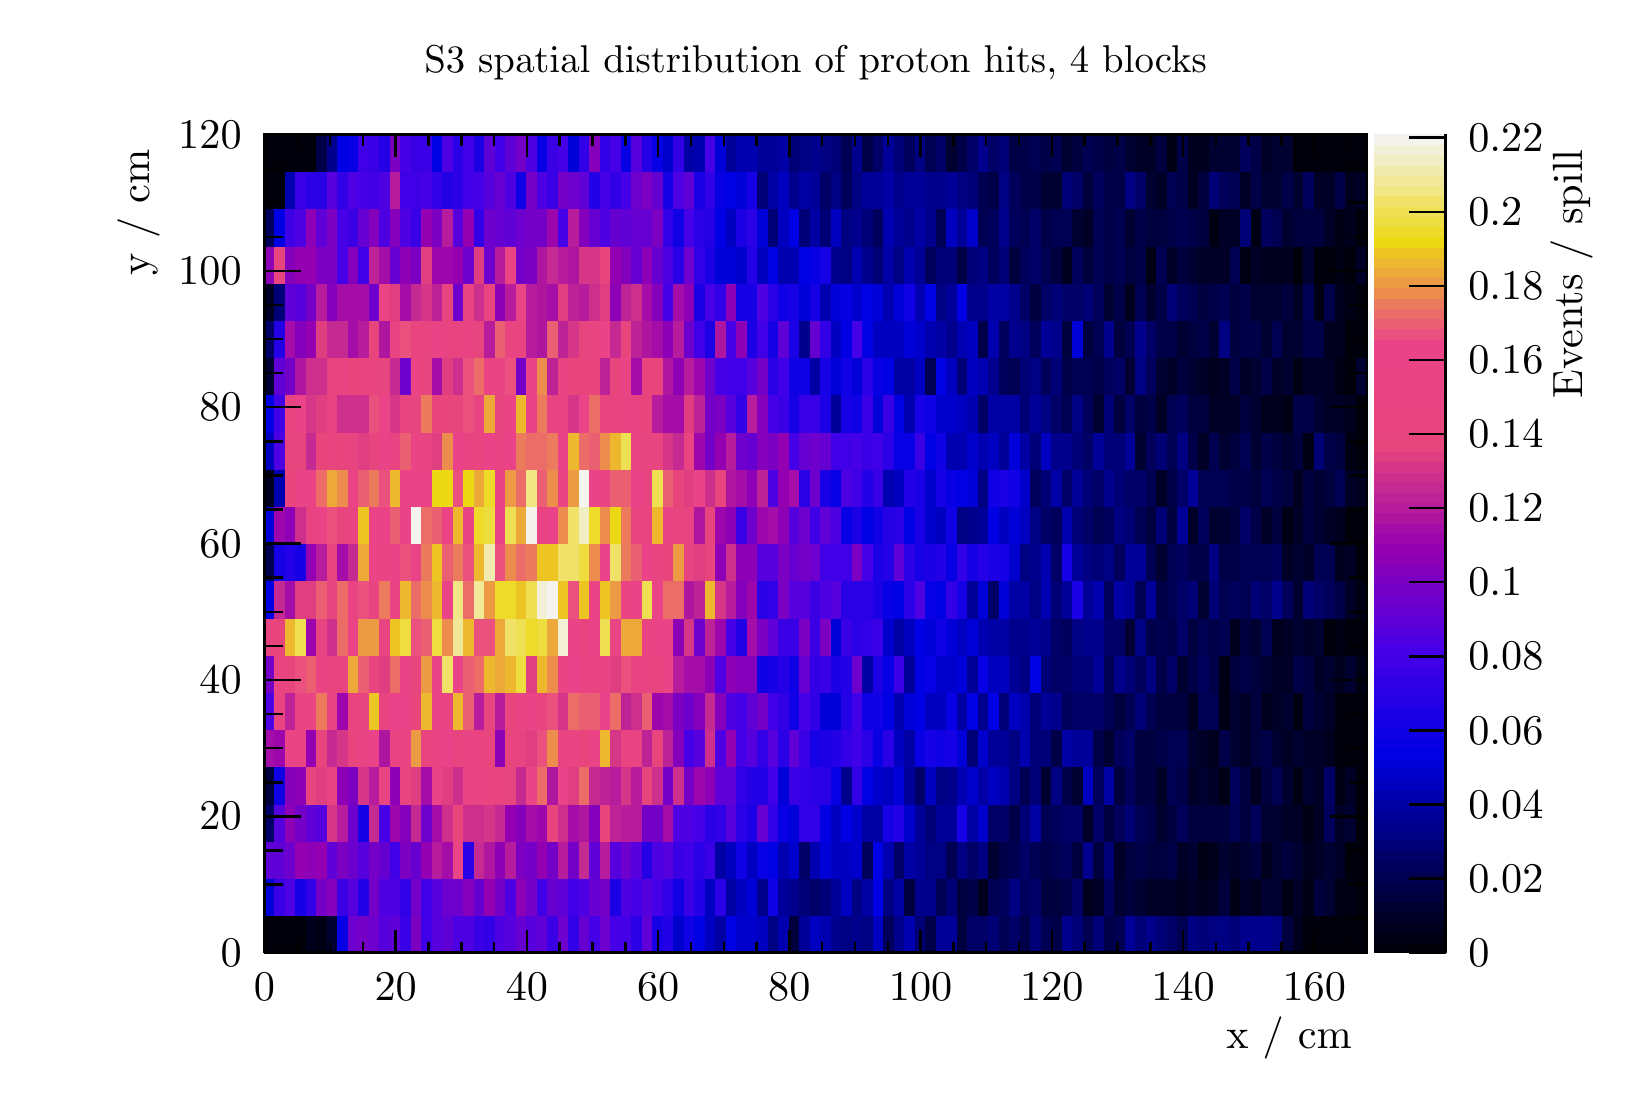
\begin{tikzpicture}
\pgfdeclareplotmark{cross} {
\pgfpathmoveto{\pgfpoint{-0.3\pgfplotmarksize}{\pgfplotmarksize}}
\pgfpathlineto{\pgfpoint{+0.3\pgfplotmarksize}{\pgfplotmarksize}}
\pgfpathlineto{\pgfpoint{+0.3\pgfplotmarksize}{0.3\pgfplotmarksize}}
\pgfpathlineto{\pgfpoint{+1\pgfplotmarksize}{0.3\pgfplotmarksize}}
\pgfpathlineto{\pgfpoint{+1\pgfplotmarksize}{-0.3\pgfplotmarksize}}
\pgfpathlineto{\pgfpoint{+0.3\pgfplotmarksize}{-0.3\pgfplotmarksize}}
\pgfpathlineto{\pgfpoint{+0.3\pgfplotmarksize}{-1.\pgfplotmarksize}}
\pgfpathlineto{\pgfpoint{-0.3\pgfplotmarksize}{-1.\pgfplotmarksize}}
\pgfpathlineto{\pgfpoint{-0.3\pgfplotmarksize}{-0.3\pgfplotmarksize}}
\pgfpathlineto{\pgfpoint{-1.\pgfplotmarksize}{-0.3\pgfplotmarksize}}
\pgfpathlineto{\pgfpoint{-1.\pgfplotmarksize}{0.3\pgfplotmarksize}}
\pgfpathlineto{\pgfpoint{-0.3\pgfplotmarksize}{0.3\pgfplotmarksize}}
\pgfpathclose
\pgfusepathqstroke
}
\pgfdeclareplotmark{cross*} {
\pgfpathmoveto{\pgfpoint{-0.3\pgfplotmarksize}{\pgfplotmarksize}}
\pgfpathlineto{\pgfpoint{+0.3\pgfplotmarksize}{\pgfplotmarksize}}
\pgfpathlineto{\pgfpoint{+0.3\pgfplotmarksize}{0.3\pgfplotmarksize}}
\pgfpathlineto{\pgfpoint{+1\pgfplotmarksize}{0.3\pgfplotmarksize}}
\pgfpathlineto{\pgfpoint{+1\pgfplotmarksize}{-0.3\pgfplotmarksize}}
\pgfpathlineto{\pgfpoint{+0.3\pgfplotmarksize}{-0.3\pgfplotmarksize}}
\pgfpathlineto{\pgfpoint{+0.3\pgfplotmarksize}{-1.\pgfplotmarksize}}
\pgfpathlineto{\pgfpoint{-0.3\pgfplotmarksize}{-1.\pgfplotmarksize}}
\pgfpathlineto{\pgfpoint{-0.3\pgfplotmarksize}{-0.3\pgfplotmarksize}}
\pgfpathlineto{\pgfpoint{-1.\pgfplotmarksize}{-0.3\pgfplotmarksize}}
\pgfpathlineto{\pgfpoint{-1.\pgfplotmarksize}{0.3\pgfplotmarksize}}
\pgfpathlineto{\pgfpoint{-0.3\pgfplotmarksize}{0.3\pgfplotmarksize}}
\pgfpathclose
\pgfusepathqfillstroke
}
\pgfdeclareplotmark{newstar} {
\pgfpathmoveto{\pgfqpoint{0pt}{\pgfplotmarksize}}
\pgfpathlineto{\pgfqpointpolar{44}{0.5\pgfplotmarksize}}
\pgfpathlineto{\pgfqpointpolar{18}{\pgfplotmarksize}}
\pgfpathlineto{\pgfqpointpolar{-20}{0.5\pgfplotmarksize}}
\pgfpathlineto{\pgfqpointpolar{-54}{\pgfplotmarksize}}
\pgfpathlineto{\pgfqpointpolar{-90}{0.5\pgfplotmarksize}}
\pgfpathlineto{\pgfqpointpolar{234}{\pgfplotmarksize}}
\pgfpathlineto{\pgfqpointpolar{198}{0.5\pgfplotmarksize}}
\pgfpathlineto{\pgfqpointpolar{162}{\pgfplotmarksize}}
\pgfpathlineto{\pgfqpointpolar{134}{0.5\pgfplotmarksize}}
\pgfpathclose
\pgfusepathqstroke
}
\pgfdeclareplotmark{newstar*} {
\pgfpathmoveto{\pgfqpoint{0pt}{\pgfplotmarksize}}
\pgfpathlineto{\pgfqpointpolar{44}{0.5\pgfplotmarksize}}
\pgfpathlineto{\pgfqpointpolar{18}{\pgfplotmarksize}}
\pgfpathlineto{\pgfqpointpolar{-20}{0.5\pgfplotmarksize}}
\pgfpathlineto{\pgfqpointpolar{-54}{\pgfplotmarksize}}
\pgfpathlineto{\pgfqpointpolar{-90}{0.5\pgfplotmarksize}}
\pgfpathlineto{\pgfqpointpolar{234}{\pgfplotmarksize}}
\pgfpathlineto{\pgfqpointpolar{198}{0.5\pgfplotmarksize}}
\pgfpathlineto{\pgfqpointpolar{162}{\pgfplotmarksize}}
\pgfpathlineto{\pgfqpointpolar{134}{0.5\pgfplotmarksize}}
\pgfpathclose
\pgfusepathqfillstroke
}
\definecolor{c}{rgb}{1,1,1};
\draw [color=c, fill=c] (0,0) rectangle (20,13.4957);
\draw [color=c, fill=c] (3,1.75444) rectangle (17,12.1461);
\definecolor{c}{rgb}{0,0,0};
\draw [c,line width=0.9] (3,1.75444) -- (3,12.1461) -- (17,12.1461) -- (17,1.75444) -- (3,1.75444);
\definecolor{c}{rgb}{1,1,1};
\draw [color=c, fill=c] (3,1.75444) rectangle (17,12.1461);
\definecolor{c}{rgb}{0,0,0};
\draw [c,line width=0.9] (3,1.75444) -- (3,12.1461) -- (17,12.1461) -- (17,1.75444) -- (3,1.75444);
\definecolor{c}{rgb}{0,0,0.0387097};
\draw [color=c, fill=c] (3,1.75444) rectangle (3.13333,2.22679);
\draw [color=c, fill=c] (3.13333,1.75444) rectangle (3.26667,2.22679);
\draw [color=c, fill=c] (3.26667,1.75444) rectangle (3.4,2.22679);
\draw [color=c, fill=c] (3.4,1.75444) rectangle (3.53333,2.22679);
\definecolor{c}{rgb}{0,0,0.116129};
\draw [color=c, fill=c] (3.53333,1.75444) rectangle (3.66667,2.22679);
\definecolor{c}{rgb}{0,0,0.0774194};
\draw [color=c, fill=c] (3.66667,1.75444) rectangle (3.8,2.22679);
\definecolor{c}{rgb}{0,0,0.193548};
\draw [color=c, fill=c] (3.8,1.75444) rectangle (3.93333,2.22679);
\definecolor{c}{rgb}{0.0257353,0,0.895221};
\draw [color=c, fill=c] (3.93333,1.75444) rectangle (4.06667,2.22679);
\definecolor{c}{rgb}{0.427451,0,0.8};
\draw [color=c, fill=c] (4.06667,1.75444) rectangle (4.2,2.22679);
\definecolor{c}{rgb}{0.456127,0,0.780147};
\draw [color=c, fill=c] (4.2,1.75444) rectangle (4.33333,2.22679);
\definecolor{c}{rgb}{0.427451,0,0.8};
\draw [color=c, fill=c] (4.33333,1.75444) rectangle (4.46667,2.22679);
\definecolor{c}{rgb}{0.331863,0,0.866176};
\draw [color=c, fill=c] (4.46667,1.75444) rectangle (4.6,2.22679);
\definecolor{c}{rgb}{0.370098,0,0.839706};
\draw [color=c, fill=c] (4.6,1.75444) rectangle (4.73333,2.22679);
\definecolor{c}{rgb}{0.223039,0,0.903676};
\draw [color=c, fill=c] (4.73333,1.75444) rectangle (4.86667,2.22679);
\definecolor{c}{rgb}{0.484804,0,0.760294};
\draw [color=c, fill=c] (4.86667,1.75444) rectangle (5,2.22679);
\definecolor{c}{rgb}{0.248775,0,0.904779};
\draw [color=c, fill=c] (5,1.75444) rectangle (5.13333,2.22679);
\definecolor{c}{rgb}{0.331863,0,0.866176};
\draw [color=c, fill=c] (5.13333,1.75444) rectangle (5.26667,2.22679);
\definecolor{c}{rgb}{0.370098,0,0.839706};
\draw [color=c, fill=c] (5.26667,1.75444) rectangle (5.4,2.22679);
\definecolor{c}{rgb}{0.303186,0,0.886029};
\draw [color=c, fill=c] (5.4,1.75444) rectangle (5.53333,2.22679);
\draw [color=c, fill=c] (5.53333,1.75444) rectangle (5.66667,2.22679);
\definecolor{c}{rgb}{0.223039,0,0.903676};
\draw [color=c, fill=c] (5.66667,1.75444) rectangle (5.8,2.22679);
\definecolor{c}{rgb}{0.197304,0,0.902574};
\draw [color=c, fill=c] (5.8,1.75444) rectangle (5.93333,2.22679);
\definecolor{c}{rgb}{0.303186,0,0.886029};
\draw [color=c, fill=c] (5.93333,1.75444) rectangle (6.06667,2.22679);
\definecolor{c}{rgb}{0.331863,0,0.866176};
\draw [color=c, fill=c] (6.06667,1.75444) rectangle (6.2,2.22679);
\definecolor{c}{rgb}{0.398775,0,0.819853};
\draw [color=c, fill=c] (6.2,1.75444) rectangle (6.33333,2.22679);
\definecolor{c}{rgb}{0.331863,0,0.866176};
\draw [color=c, fill=c] (6.33333,1.75444) rectangle (6.46667,2.22679);
\definecolor{c}{rgb}{0.370098,0,0.839706};
\draw [color=c, fill=c] (6.46667,1.75444) rectangle (6.6,2.22679);
\definecolor{c}{rgb}{0.223039,0,0.903676};
\draw [color=c, fill=c] (6.6,1.75444) rectangle (6.73333,2.22679);
\definecolor{c}{rgb}{0.427451,0,0.8};
\draw [color=c, fill=c] (6.73333,1.75444) rectangle (6.86667,2.22679);
\definecolor{c}{rgb}{0.197304,0,0.902574};
\draw [color=c, fill=c] (6.86667,1.75444) rectangle (7,2.22679);
\definecolor{c}{rgb}{0.398775,0,0.819853};
\draw [color=c, fill=c] (7,1.75444) rectangle (7.13333,2.22679);
\definecolor{c}{rgb}{0.27451,0,0.905882};
\draw [color=c, fill=c] (7.13333,1.75444) rectangle (7.26667,2.22679);
\definecolor{c}{rgb}{0.427451,0,0.8};
\draw [color=c, fill=c] (7.26667,1.75444) rectangle (7.4,2.22679);
\definecolor{c}{rgb}{0.27451,0,0.905882};
\draw [color=c, fill=c] (7.4,1.75444) rectangle (7.53333,2.22679);
\draw [color=c, fill=c] (7.53333,1.75444) rectangle (7.66667,2.22679);
\definecolor{c}{rgb}{0.16299,0,0.901103};
\draw [color=c, fill=c] (7.66667,1.75444) rectangle (7.8,2.22679);
\definecolor{c}{rgb}{0.370098,0,0.839706};
\draw [color=c, fill=c] (7.8,1.75444) rectangle (7.93333,2.22679);
\definecolor{c}{rgb}{0.0857843,0,0.897794};
\draw [color=c, fill=c] (7.93333,1.75444) rectangle (8.06667,2.22679);
\definecolor{c}{rgb}{0.137255,0,0.9};
\draw [color=c, fill=c] (8.06667,1.75444) rectangle (8.2,2.22679);
\definecolor{c}{rgb}{0,0,0.801471};
\draw [color=c, fill=c] (8.2,1.75444) rectangle (8.33333,2.22679);
\definecolor{c}{rgb}{0.060049,0,0.896691};
\draw [color=c, fill=c] (8.33333,1.75444) rectangle (8.46667,2.22679);
\definecolor{c}{rgb}{0,0,0.894118};
\draw [color=c, fill=c] (8.46667,1.75444) rectangle (8.6,2.22679);
\definecolor{c}{rgb}{0,0,0.755147};
\draw [color=c, fill=c] (8.6,1.75444) rectangle (8.73333,2.22679);
\definecolor{c}{rgb}{0,0,0.647059};
\draw [color=c, fill=c] (8.73333,1.75444) rectangle (8.86667,2.22679);
\definecolor{c}{rgb}{0,0,0.894118};
\draw [color=c, fill=c] (8.86667,1.75444) rectangle (9,2.22679);
\definecolor{c}{rgb}{0,0,0.801471};
\draw [color=c, fill=c] (9,1.75444) rectangle (9.13333,2.22679);
\draw [color=c, fill=c] (9.13333,1.75444) rectangle (9.26667,2.22679);
\definecolor{c}{rgb}{0,0,0.755147};
\draw [color=c, fill=c] (9.26667,1.75444) rectangle (9.4,2.22679);
\definecolor{c}{rgb}{0,0,0.508088};
\draw [color=c, fill=c] (9.4,1.75444) rectangle (9.53333,2.22679);
\definecolor{c}{rgb}{0,0,0.693382};
\draw [color=c, fill=c] (9.53333,1.75444) rectangle (9.66667,2.22679);
\definecolor{c}{rgb}{0,0,0.245161};
\draw [color=c, fill=c] (9.66667,1.75444) rectangle (9.8,2.22679);
\definecolor{c}{rgb}{0,0,0.600735};
\draw [color=c, fill=c] (9.8,1.75444) rectangle (9.93333,2.22679);
\definecolor{c}{rgb}{0,0,0.755147};
\draw [color=c, fill=c] (9.93333,1.75444) rectangle (10.0667,2.22679);
\definecolor{c}{rgb}{0,0,0.693382};
\draw [color=c, fill=c] (10.0667,1.75444) rectangle (10.2,2.22679);
\definecolor{c}{rgb}{0,0,0.554412};
\draw [color=c, fill=c] (10.2,1.75444) rectangle (10.3333,2.22679);
\definecolor{c}{rgb}{0,0,0.508088};
\draw [color=c, fill=c] (10.3333,1.75444) rectangle (10.4667,2.22679);
\definecolor{c}{rgb}{0,0,0.554412};
\draw [color=c, fill=c] (10.4667,1.75444) rectangle (10.6,2.22679);
\definecolor{c}{rgb}{0,0,0.508088};
\draw [color=c, fill=c] (10.6,1.75444) rectangle (10.7333,2.22679);
\definecolor{c}{rgb}{0,0,0.755147};
\draw [color=c, fill=c] (10.7333,1.75444) rectangle (10.8667,2.22679);
\definecolor{c}{rgb}{0,0,0.36129};
\draw [color=c, fill=c] (10.8667,1.75444) rectangle (11,2.22679);
\definecolor{c}{rgb}{0,0,0.554412};
\draw [color=c, fill=c] (11,1.75444) rectangle (11.1333,2.22679);
\definecolor{c}{rgb}{0,0,0.693382};
\draw [color=c, fill=c] (11.1333,1.75444) rectangle (11.2667,2.22679);
\definecolor{c}{rgb}{0,0,0.461765};
\draw [color=c, fill=c] (11.2667,1.75444) rectangle (11.4,2.22679);
\definecolor{c}{rgb}{0,0,0.283871};
\draw [color=c, fill=c] (11.4,1.75444) rectangle (11.5333,2.22679);
\definecolor{c}{rgb}{0,0,0.600735};
\draw [color=c, fill=c] (11.5333,1.75444) rectangle (11.6667,2.22679);
\draw [color=c, fill=c] (11.6667,1.75444) rectangle (11.8,2.22679);
\definecolor{c}{rgb}{0,0,0.245161};
\draw [color=c, fill=c] (11.8,1.75444) rectangle (11.9333,2.22679);
\definecolor{c}{rgb}{0,0,0.4};
\draw [color=c, fill=c] (11.9333,1.75444) rectangle (12.0667,2.22679);
\draw [color=c, fill=c] (12.0667,1.75444) rectangle (12.2,2.22679);
\definecolor{c}{rgb}{0,0,0.461765};
\draw [color=c, fill=c] (12.2,1.75444) rectangle (12.3333,2.22679);
\definecolor{c}{rgb}{0,0,0.322581};
\draw [color=c, fill=c] (12.3333,1.75444) rectangle (12.4667,2.22679);
\definecolor{c}{rgb}{0,0,0.4};
\draw [color=c, fill=c] (12.4667,1.75444) rectangle (12.6,2.22679);
\definecolor{c}{rgb}{0,0,0.283871};
\draw [color=c, fill=c] (12.6,1.75444) rectangle (12.7333,2.22679);
\definecolor{c}{rgb}{0,0,0.461765};
\draw [color=c, fill=c] (12.7333,1.75444) rectangle (12.8667,2.22679);
\definecolor{c}{rgb}{0,0,0.322581};
\draw [color=c, fill=c] (12.8667,1.75444) rectangle (13,2.22679);
\definecolor{c}{rgb}{0,0,0.283871};
\draw [color=c, fill=c] (13,1.75444) rectangle (13.1333,2.22679);
\definecolor{c}{rgb}{0,0,0.554412};
\draw [color=c, fill=c] (13.1333,1.75444) rectangle (13.2667,2.22679);
\definecolor{c}{rgb}{0,0,0.461765};
\draw [color=c, fill=c] (13.2667,1.75444) rectangle (13.4,2.22679);
\definecolor{c}{rgb}{0,0,0.322581};
\draw [color=c, fill=c] (13.4,1.75444) rectangle (13.5333,2.22679);
\definecolor{c}{rgb}{0,0,0.461765};
\draw [color=c, fill=c] (13.5333,1.75444) rectangle (13.6667,2.22679);
\definecolor{c}{rgb}{0,0,0.283871};
\draw [color=c, fill=c] (13.6667,1.75444) rectangle (13.8,2.22679);
\definecolor{c}{rgb}{0,0,0.322581};
\draw [color=c, fill=c] (13.8,1.75444) rectangle (13.9333,2.22679);
\definecolor{c}{rgb}{0,0,0.600735};
\draw [color=c, fill=c] (13.9333,1.75444) rectangle (14.0667,2.22679);
\definecolor{c}{rgb}{0,0,0.461765};
\draw [color=c, fill=c] (14.0667,1.75444) rectangle (14.2,2.22679);
\definecolor{c}{rgb}{0,0,0.554412};
\draw [color=c, fill=c] (14.2,1.75444) rectangle (14.3333,2.22679);
\definecolor{c}{rgb}{0,0,0.461765};
\draw [color=c, fill=c] (14.3333,1.75444) rectangle (14.4667,2.22679);
\definecolor{c}{rgb}{0,0,0.4};
\draw [color=c, fill=c] (14.4667,1.75444) rectangle (14.6,2.22679);
\definecolor{c}{rgb}{0,0,0.322581};
\draw [color=c, fill=c] (14.6,1.75444) rectangle (14.7333,2.22679);
\definecolor{c}{rgb}{0,0,0.508088};
\draw [color=c, fill=c] (14.7333,1.75444) rectangle (14.8667,2.22679);
\definecolor{c}{rgb}{0,0,0.461765};
\draw [color=c, fill=c] (14.8667,1.75444) rectangle (15,2.22679);
\definecolor{c}{rgb}{0,0,0.508088};
\draw [color=c, fill=c] (15,1.75444) rectangle (15.1333,2.22679);
\draw [color=c, fill=c] (15.1333,1.75444) rectangle (15.2667,2.22679);
\definecolor{c}{rgb}{0,0,0.461765};
\draw [color=c, fill=c] (15.2667,1.75444) rectangle (15.4,2.22679);
\definecolor{c}{rgb}{0,0,0.554412};
\draw [color=c, fill=c] (15.4,1.75444) rectangle (15.5333,2.22679);
\draw [color=c, fill=c] (15.5333,1.75444) rectangle (15.6667,2.22679);
\draw [color=c, fill=c] (15.6667,1.75444) rectangle (15.8,2.22679);
\definecolor{c}{rgb}{0,0,0.508088};
\draw [color=c, fill=c] (15.8,1.75444) rectangle (15.9333,2.22679);
\definecolor{c}{rgb}{0,0,0.245161};
\draw [color=c, fill=c] (15.9333,1.75444) rectangle (16.0667,2.22679);
\definecolor{c}{rgb}{0,0,0.116129};
\draw [color=c, fill=c] (16.0667,1.75444) rectangle (16.2,2.22679);
\definecolor{c}{rgb}{0,0,0.0387097};
\draw [color=c, fill=c] (16.2,1.75444) rectangle (16.3333,2.22679);
\draw [color=c, fill=c] (16.3333,1.75444) rectangle (16.4667,2.22679);
\draw [color=c, fill=c] (16.4667,1.75444) rectangle (16.6,2.22679);
\draw [color=c, fill=c] (16.6,1.75444) rectangle (16.7333,2.22679);
\draw [color=c, fill=c] (16.7333,1.75444) rectangle (16.8667,2.22679);
\draw [color=c, fill=c] (16.8667,1.75444) rectangle (17,2.22679);
\definecolor{c}{rgb}{0,0,0.847794};
\draw [color=c, fill=c] (3,2.22679) rectangle (3.13333,2.69914);
\definecolor{c}{rgb}{0.223039,0,0.903676};
\draw [color=c, fill=c] (3.13333,2.22679) rectangle (3.26667,2.69914);
\definecolor{c}{rgb}{0.303186,0,0.886029};
\draw [color=c, fill=c] (3.26667,2.22679) rectangle (3.4,2.69914);
\definecolor{c}{rgb}{0.0857843,0,0.897794};
\draw [color=c, fill=c] (3.4,2.22679) rectangle (3.53333,2.69914);
\definecolor{c}{rgb}{0.197304,0,0.902574};
\draw [color=c, fill=c] (3.53333,2.22679) rectangle (3.66667,2.69914);
\definecolor{c}{rgb}{0.456127,0,0.780147};
\draw [color=c, fill=c] (3.66667,2.22679) rectangle (3.8,2.69914);
\definecolor{c}{rgb}{0.523039,0,0.733824};
\draw [color=c, fill=c] (3.8,2.22679) rectangle (3.93333,2.69914);
\definecolor{c}{rgb}{0.223039,0,0.903676};
\draw [color=c, fill=c] (3.93333,2.22679) rectangle (4.06667,2.69914);
\definecolor{c}{rgb}{0.331863,0,0.866176};
\draw [color=c, fill=c] (4.06667,2.22679) rectangle (4.2,2.69914);
\definecolor{c}{rgb}{0.137255,0,0.9};
\draw [color=c, fill=c] (4.2,2.22679) rectangle (4.33333,2.69914);
\definecolor{c}{rgb}{0.456127,0,0.780147};
\draw [color=c, fill=c] (4.33333,2.22679) rectangle (4.46667,2.69914);
\definecolor{c}{rgb}{0.303186,0,0.886029};
\draw [color=c, fill=c] (4.46667,2.22679) rectangle (4.6,2.69914);
\draw [color=c, fill=c] (4.6,2.22679) rectangle (4.73333,2.69914);
\definecolor{c}{rgb}{0.197304,0,0.902574};
\draw [color=c, fill=c] (4.73333,2.22679) rectangle (4.86667,2.69914);
\definecolor{c}{rgb}{0.456127,0,0.780147};
\draw [color=c, fill=c] (4.86667,2.22679) rectangle (5,2.69914);
\definecolor{c}{rgb}{0.248775,0,0.904779};
\draw [color=c, fill=c] (5,2.22679) rectangle (5.13333,2.69914);
\definecolor{c}{rgb}{0.331863,0,0.866176};
\draw [color=c, fill=c] (5.13333,2.22679) rectangle (5.26667,2.69914);
\definecolor{c}{rgb}{0.427451,0,0.8};
\draw [color=c, fill=c] (5.26667,2.22679) rectangle (5.4,2.69914);
\draw [color=c, fill=c] (5.4,2.22679) rectangle (5.53333,2.69914);
\definecolor{c}{rgb}{0.523039,0,0.733824};
\draw [color=c, fill=c] (5.53333,2.22679) rectangle (5.66667,2.69914);
\definecolor{c}{rgb}{0.398775,0,0.819853};
\draw [color=c, fill=c] (5.66667,2.22679) rectangle (5.8,2.69914);
\definecolor{c}{rgb}{0.580392,0,0.694118};
\draw [color=c, fill=c] (5.8,2.22679) rectangle (5.93333,2.69914);
\definecolor{c}{rgb}{0.456127,0,0.780147};
\draw [color=c, fill=c] (5.93333,2.22679) rectangle (6.06667,2.69914);
\definecolor{c}{rgb}{0.303186,0,0.886029};
\draw [color=c, fill=c] (6.06667,2.22679) rectangle (6.2,2.69914);
\definecolor{c}{rgb}{0.551716,0,0.713971};
\draw [color=c, fill=c] (6.2,2.22679) rectangle (6.33333,2.69914);
\definecolor{c}{rgb}{0.456127,0,0.780147};
\draw [color=c, fill=c] (6.33333,2.22679) rectangle (6.46667,2.69914);
\definecolor{c}{rgb}{0.248775,0,0.904779};
\draw [color=c, fill=c] (6.46667,2.22679) rectangle (6.6,2.69914);
\definecolor{c}{rgb}{0.398775,0,0.819853};
\draw [color=c, fill=c] (6.6,2.22679) rectangle (6.73333,2.69914);
\definecolor{c}{rgb}{0.370098,0,0.839706};
\draw [color=c, fill=c] (6.73333,2.22679) rectangle (6.86667,2.69914);
\definecolor{c}{rgb}{0.248775,0,0.904779};
\draw [color=c, fill=c] (6.86667,2.22679) rectangle (7,2.69914);
\definecolor{c}{rgb}{0.303186,0,0.886029};
\draw [color=c, fill=c] (7,2.22679) rectangle (7.13333,2.69914);
\definecolor{c}{rgb}{0.398775,0,0.819853};
\draw [color=c, fill=c] (7.13333,2.22679) rectangle (7.26667,2.69914);
\definecolor{c}{rgb}{0.456127,0,0.780147};
\draw [color=c, fill=c] (7.26667,2.22679) rectangle (7.4,2.69914);
\definecolor{c}{rgb}{0.11152,0,0.898897};
\draw [color=c, fill=c] (7.4,2.22679) rectangle (7.53333,2.69914);
\definecolor{c}{rgb}{0.303186,0,0.886029};
\draw [color=c, fill=c] (7.53333,2.22679) rectangle (7.66667,2.69914);
\definecolor{c}{rgb}{0.27451,0,0.905882};
\draw [color=c, fill=c] (7.66667,2.22679) rectangle (7.8,2.69914);
\definecolor{c}{rgb}{0.331863,0,0.866176};
\draw [color=c, fill=c] (7.8,2.22679) rectangle (7.93333,2.69914);
\definecolor{c}{rgb}{0.27451,0,0.905882};
\draw [color=c, fill=c] (7.93333,2.22679) rectangle (8.06667,2.69914);
\definecolor{c}{rgb}{0.197304,0,0.902574};
\draw [color=c, fill=c] (8.06667,2.22679) rectangle (8.2,2.69914);
\definecolor{c}{rgb}{0.060049,0,0.896691};
\draw [color=c, fill=c] (8.2,2.22679) rectangle (8.33333,2.69914);
\definecolor{c}{rgb}{0.223039,0,0.903676};
\draw [color=c, fill=c] (8.33333,2.22679) rectangle (8.46667,2.69914);
\definecolor{c}{rgb}{0.137255,0,0.9};
\draw [color=c, fill=c] (8.46667,2.22679) rectangle (8.6,2.69914);
\definecolor{c}{rgb}{0,0,0.755147};
\draw [color=c, fill=c] (8.6,2.22679) rectangle (8.73333,2.69914);
\definecolor{c}{rgb}{0.16299,0,0.901103};
\draw [color=c, fill=c] (8.73333,2.22679) rectangle (8.86667,2.69914);
\definecolor{c}{rgb}{0,0,0.647059};
\draw [color=c, fill=c] (8.86667,2.22679) rectangle (9,2.69914);
\definecolor{c}{rgb}{0,0,0.755147};
\draw [color=c, fill=c] (9,2.22679) rectangle (9.13333,2.69914);
\definecolor{c}{rgb}{0,0,0.847794};
\draw [color=c, fill=c] (9.13333,2.22679) rectangle (9.26667,2.69914);
\definecolor{c}{rgb}{0,0,0.554412};
\draw [color=c, fill=c] (9.26667,2.22679) rectangle (9.4,2.69914);
\definecolor{c}{rgb}{0.060049,0,0.896691};
\draw [color=c, fill=c] (9.4,2.22679) rectangle (9.53333,2.69914);
\definecolor{c}{rgb}{0,0,0.600735};
\draw [color=c, fill=c] (9.53333,2.22679) rectangle (9.66667,2.69914);
\definecolor{c}{rgb}{0,0,0.554412};
\draw [color=c, fill=c] (9.66667,2.22679) rectangle (9.8,2.69914);
\definecolor{c}{rgb}{0,0,0.461765};
\draw [color=c, fill=c] (9.8,2.22679) rectangle (9.93333,2.69914);
\definecolor{c}{rgb}{0,0,0.4};
\draw [color=c, fill=c] (9.93333,2.22679) rectangle (10.0667,2.69914);
\definecolor{c}{rgb}{0,0,0.461765};
\draw [color=c, fill=c] (10.0667,2.22679) rectangle (10.2,2.69914);
\definecolor{c}{rgb}{0,0,0.600735};
\draw [color=c, fill=c] (10.2,2.22679) rectangle (10.3333,2.69914);
\definecolor{c}{rgb}{0,0,0.755147};
\draw [color=c, fill=c] (10.3333,2.22679) rectangle (10.4667,2.69914);
\definecolor{c}{rgb}{0,0,0.508088};
\draw [color=c, fill=c] (10.4667,2.22679) rectangle (10.6,2.69914);
\definecolor{c}{rgb}{0,0,0.647059};
\draw [color=c, fill=c] (10.6,2.22679) rectangle (10.7333,2.69914);
\definecolor{c}{rgb}{0,0,0.894118};
\draw [color=c, fill=c] (10.7333,2.22679) rectangle (10.8667,2.69914);
\definecolor{c}{rgb}{0,0,0.508088};
\draw [color=c, fill=c] (10.8667,2.22679) rectangle (11,2.69914);
\definecolor{c}{rgb}{0,0,0.647059};
\draw [color=c, fill=c] (11,2.22679) rectangle (11.1333,2.69914);
\definecolor{c}{rgb}{0,0,0.245161};
\draw [color=c, fill=c] (11.1333,2.22679) rectangle (11.2667,2.69914);
\definecolor{c}{rgb}{0,0,0.554412};
\draw [color=c, fill=c] (11.2667,2.22679) rectangle (11.4,2.69914);
\draw [color=c, fill=c] (11.4,2.22679) rectangle (11.5333,2.69914);
\definecolor{c}{rgb}{0,0,0.322581};
\draw [color=c, fill=c] (11.5333,2.22679) rectangle (11.6667,2.69914);
\definecolor{c}{rgb}{0,0,0.461765};
\draw [color=c, fill=c] (11.6667,2.22679) rectangle (11.8,2.69914);
\definecolor{c}{rgb}{0,0,0.245161};
\draw [color=c, fill=c] (11.8,2.22679) rectangle (11.9333,2.69914);
\definecolor{c}{rgb}{0,0,0.283871};
\draw [color=c, fill=c] (11.9333,2.22679) rectangle (12.0667,2.69914);
\definecolor{c}{rgb}{0,0,0.116129};
\draw [color=c, fill=c] (12.0667,2.22679) rectangle (12.2,2.69914);
\definecolor{c}{rgb}{0,0,0.322581};
\draw [color=c, fill=c] (12.2,2.22679) rectangle (12.3333,2.69914);
\definecolor{c}{rgb}{0,0,0.36129};
\draw [color=c, fill=c] (12.3333,2.22679) rectangle (12.4667,2.69914);
\definecolor{c}{rgb}{0,0,0.508088};
\draw [color=c, fill=c] (12.4667,2.22679) rectangle (12.6,2.69914);
\definecolor{c}{rgb}{0,0,0.36129};
\draw [color=c, fill=c] (12.6,2.22679) rectangle (12.7333,2.69914);
\definecolor{c}{rgb}{0,0,0.4};
\draw [color=c, fill=c] (12.7333,2.22679) rectangle (12.8667,2.69914);
\definecolor{c}{rgb}{0,0,0.245161};
\draw [color=c, fill=c] (12.8667,2.22679) rectangle (13,2.69914);
\draw [color=c, fill=c] (13,2.22679) rectangle (13.1333,2.69914);
\definecolor{c}{rgb}{0,0,0.283871};
\draw [color=c, fill=c] (13.1333,2.22679) rectangle (13.2667,2.69914);
\definecolor{c}{rgb}{0,0,0.4};
\draw [color=c, fill=c] (13.2667,2.22679) rectangle (13.4,2.69914);
\definecolor{c}{rgb}{0,0,0.116129};
\draw [color=c, fill=c] (13.4,2.22679) rectangle (13.5333,2.69914);
\definecolor{c}{rgb}{0,0,0.154839};
\draw [color=c, fill=c] (13.5333,2.22679) rectangle (13.6667,2.69914);
\definecolor{c}{rgb}{0,0,0.36129};
\draw [color=c, fill=c] (13.6667,2.22679) rectangle (13.8,2.69914);
\definecolor{c}{rgb}{0,0,0.193548};
\draw [color=c, fill=c] (13.8,2.22679) rectangle (13.9333,2.69914);
\definecolor{c}{rgb}{0,0,0.245161};
\draw [color=c, fill=c] (13.9333,2.22679) rectangle (14.0667,2.69914);
\definecolor{c}{rgb}{0,0,0.193548};
\draw [color=c, fill=c] (14.0667,2.22679) rectangle (14.2,2.69914);
\definecolor{c}{rgb}{0,0,0.154839};
\draw [color=c, fill=c] (14.2,2.22679) rectangle (14.3333,2.69914);
\draw [color=c, fill=c] (14.3333,2.22679) rectangle (14.4667,2.69914);
\draw [color=c, fill=c] (14.4667,2.22679) rectangle (14.6,2.69914);
\definecolor{c}{rgb}{0,0,0.116129};
\draw [color=c, fill=c] (14.6,2.22679) rectangle (14.7333,2.69914);
\definecolor{c}{rgb}{0,0,0.154839};
\draw [color=c, fill=c] (14.7333,2.22679) rectangle (14.8667,2.69914);
\definecolor{c}{rgb}{0,0,0.116129};
\draw [color=c, fill=c] (14.8667,2.22679) rectangle (15,2.69914);
\definecolor{c}{rgb}{0,0,0.154839};
\draw [color=c, fill=c] (15,2.22679) rectangle (15.1333,2.69914);
\definecolor{c}{rgb}{0,0,0.245161};
\draw [color=c, fill=c] (15.1333,2.22679) rectangle (15.2667,2.69914);
\definecolor{c}{rgb}{0,0,0.0774194};
\draw [color=c, fill=c] (15.2667,2.22679) rectangle (15.4,2.69914);
\definecolor{c}{rgb}{0,0,0.154839};
\draw [color=c, fill=c] (15.4,2.22679) rectangle (15.5333,2.69914);
\definecolor{c}{rgb}{0,0,0.116129};
\draw [color=c, fill=c] (15.5333,2.22679) rectangle (15.6667,2.69914);
\definecolor{c}{rgb}{0,0,0.193548};
\draw [color=c, fill=c] (15.6667,2.22679) rectangle (15.8,2.69914);
\draw [color=c, fill=c] (15.8,2.22679) rectangle (15.9333,2.69914);
\definecolor{c}{rgb}{0,0,0.0774194};
\draw [color=c, fill=c] (15.9333,2.22679) rectangle (16.0667,2.69914);
\definecolor{c}{rgb}{0,0,0.154839};
\draw [color=c, fill=c] (16.0667,2.22679) rectangle (16.2,2.69914);
\definecolor{c}{rgb}{0,0,0.0774194};
\draw [color=c, fill=c] (16.2,2.22679) rectangle (16.3333,2.69914);
\definecolor{c}{rgb}{0,0,0.245161};
\draw [color=c, fill=c] (16.3333,2.22679) rectangle (16.4667,2.69914);
\definecolor{c}{rgb}{0,0,0.193548};
\draw [color=c, fill=c] (16.4667,2.22679) rectangle (16.6,2.69914);
\definecolor{c}{rgb}{0,0,0.0774194};
\draw [color=c, fill=c] (16.6,2.22679) rectangle (16.7333,2.69914);
\draw [color=c, fill=c] (16.7333,2.22679) rectangle (16.8667,2.69914);
\definecolor{c}{rgb}{0,0,0.0387097};
\draw [color=c, fill=c] (16.8667,2.22679) rectangle (17,2.69914);
\definecolor{c}{rgb}{0.370098,0,0.839706};
\draw [color=c, fill=c] (3,2.69914) rectangle (3.13333,3.17149);
\draw [color=c, fill=c] (3.13333,2.69914) rectangle (3.26667,3.17149);
\definecolor{c}{rgb}{0.427451,0,0.8};
\draw [color=c, fill=c] (3.26667,2.69914) rectangle (3.4,3.17149);
\definecolor{c}{rgb}{0.580392,0,0.694118};
\draw [color=c, fill=c] (3.4,2.69914) rectangle (3.53333,3.17149);
\definecolor{c}{rgb}{0.551716,0,0.713971};
\draw [color=c, fill=c] (3.53333,2.69914) rectangle (3.66667,3.17149);
\definecolor{c}{rgb}{0.580392,0,0.694118};
\draw [color=c, fill=c] (3.66667,2.69914) rectangle (3.8,3.17149);
\definecolor{c}{rgb}{0.370098,0,0.839706};
\draw [color=c, fill=c] (3.8,2.69914) rectangle (3.93333,3.17149);
\definecolor{c}{rgb}{0.484804,0,0.760294};
\draw [color=c, fill=c] (3.93333,2.69914) rectangle (4.06667,3.17149);
\definecolor{c}{rgb}{0.427451,0,0.8};
\draw [color=c, fill=c] (4.06667,2.69914) rectangle (4.2,3.17149);
\definecolor{c}{rgb}{0.331863,0,0.866176};
\draw [color=c, fill=c] (4.2,2.69914) rectangle (4.33333,3.17149);
\definecolor{c}{rgb}{0.456127,0,0.780147};
\draw [color=c, fill=c] (4.33333,2.69914) rectangle (4.46667,3.17149);
\definecolor{c}{rgb}{0.398775,0,0.819853};
\draw [color=c, fill=c] (4.46667,2.69914) rectangle (4.6,3.17149);
\definecolor{c}{rgb}{0.248775,0,0.904779};
\draw [color=c, fill=c] (4.6,2.69914) rectangle (4.73333,3.17149);
\definecolor{c}{rgb}{0.484804,0,0.760294};
\draw [color=c, fill=c] (4.73333,2.69914) rectangle (4.86667,3.17149);
\definecolor{c}{rgb}{0.398775,0,0.819853};
\draw [color=c, fill=c] (4.86667,2.69914) rectangle (5,3.17149);
\definecolor{c}{rgb}{0.580392,0,0.694118};
\draw [color=c, fill=c] (5,2.69914) rectangle (5.13333,3.17149);
\definecolor{c}{rgb}{0.712623,0.109926,0.609681};
\draw [color=c, fill=c] (5.13333,2.69914) rectangle (5.26667,3.17149);
\definecolor{c}{rgb}{0.641422,0.0507353,0.655147};
\draw [color=c, fill=c] (5.26667,2.69914) rectangle (5.4,3.17149);
\definecolor{c}{rgb}{0.915196,0.265931,0.516544};
\draw [color=c, fill=c] (5.4,2.69914) rectangle (5.53333,3.17149);
\definecolor{c}{rgb}{0.16299,0,0.901103};
\draw [color=c, fill=c] (5.53333,2.69914) rectangle (5.66667,3.17149);
\definecolor{c}{rgb}{0.773652,0.160662,0.570711};
\draw [color=c, fill=c] (5.66667,2.69914) rectangle (5.8,3.17149);
\definecolor{c}{rgb}{0.682108,0.0845588,0.629167};
\draw [color=c, fill=c] (5.8,2.69914) rectangle (5.93333,3.17149);
\definecolor{c}{rgb}{0.551716,0,0.713971};
\draw [color=c, fill=c] (5.93333,2.69914) rectangle (6.06667,3.17149);
\definecolor{c}{rgb}{0.712623,0.109926,0.609681};
\draw [color=c, fill=c] (6.06667,2.69914) rectangle (6.2,3.17149);
\definecolor{c}{rgb}{0.484804,0,0.760294};
\draw [color=c, fill=c] (6.2,2.69914) rectangle (6.33333,3.17149);
\definecolor{c}{rgb}{0.456127,0,0.780147};
\draw [color=c, fill=c] (6.33333,2.69914) rectangle (6.46667,3.17149);
\definecolor{c}{rgb}{0.580392,0,0.694118};
\draw [color=c, fill=c] (6.46667,2.69914) rectangle (6.6,3.17149);
\definecolor{c}{rgb}{0.456127,0,0.780147};
\draw [color=c, fill=c] (6.6,2.69914) rectangle (6.73333,3.17149);
\definecolor{c}{rgb}{0.712623,0.109926,0.609681};
\draw [color=c, fill=c] (6.73333,2.69914) rectangle (6.86667,3.17149);
\definecolor{c}{rgb}{0.456127,0,0.780147};
\draw [color=c, fill=c] (6.86667,2.69914) rectangle (7,3.17149);
\definecolor{c}{rgb}{0.773652,0.160662,0.570711};
\draw [color=c, fill=c] (7,2.69914) rectangle (7.13333,3.17149);
\definecolor{c}{rgb}{0.370098,0,0.839706};
\draw [color=c, fill=c] (7.13333,2.69914) rectangle (7.26667,3.17149);
\definecolor{c}{rgb}{0.712623,0.109926,0.609681};
\draw [color=c, fill=c] (7.26667,2.69914) rectangle (7.4,3.17149);
\definecolor{c}{rgb}{0.331863,0,0.866176};
\draw [color=c, fill=c] (7.4,2.69914) rectangle (7.53333,3.17149);
\definecolor{c}{rgb}{0.427451,0,0.8};
\draw [color=c, fill=c] (7.53333,2.69914) rectangle (7.66667,3.17149);
\definecolor{c}{rgb}{0.331863,0,0.866176};
\draw [color=c, fill=c] (7.66667,2.69914) rectangle (7.8,3.17149);
\definecolor{c}{rgb}{0.137255,0,0.9};
\draw [color=c, fill=c] (7.8,2.69914) rectangle (7.93333,3.17149);
\definecolor{c}{rgb}{0.303186,0,0.886029};
\draw [color=c, fill=c] (7.93333,2.69914) rectangle (8.06667,3.17149);
\definecolor{c}{rgb}{0.331863,0,0.866176};
\draw [color=c, fill=c] (8.06667,2.69914) rectangle (8.2,3.17149);
\definecolor{c}{rgb}{0.223039,0,0.903676};
\draw [color=c, fill=c] (8.2,2.69914) rectangle (8.33333,3.17149);
\definecolor{c}{rgb}{0.248775,0,0.904779};
\draw [color=c, fill=c] (8.33333,2.69914) rectangle (8.46667,3.17149);
\definecolor{c}{rgb}{0.16299,0,0.901103};
\draw [color=c, fill=c] (8.46667,2.69914) rectangle (8.6,3.17149);
\definecolor{c}{rgb}{0.223039,0,0.903676};
\draw [color=c, fill=c] (8.6,2.69914) rectangle (8.73333,3.17149);
\definecolor{c}{rgb}{0,0,0.647059};
\draw [color=c, fill=c] (8.73333,2.69914) rectangle (8.86667,3.17149);
\definecolor{c}{rgb}{0,0,0.755147};
\draw [color=c, fill=c] (8.86667,2.69914) rectangle (9,3.17149);
\definecolor{c}{rgb}{0.060049,0,0.896691};
\draw [color=c, fill=c] (9,2.69914) rectangle (9.13333,3.17149);
\definecolor{c}{rgb}{0,0,0.755147};
\draw [color=c, fill=c] (9.13333,2.69914) rectangle (9.26667,3.17149);
\definecolor{c}{rgb}{0.0257353,0,0.895221};
\draw [color=c, fill=c] (9.26667,2.69914) rectangle (9.4,3.17149);
\definecolor{c}{rgb}{0,0,0.894118};
\draw [color=c, fill=c] (9.4,2.69914) rectangle (9.53333,3.17149);
\definecolor{c}{rgb}{0,0,0.693382};
\draw [color=c, fill=c] (9.53333,2.69914) rectangle (9.66667,3.17149);
\definecolor{c}{rgb}{0,0,0.801471};
\draw [color=c, fill=c] (9.66667,2.69914) rectangle (9.8,3.17149);
\definecolor{c}{rgb}{0,0,0.4};
\draw [color=c, fill=c] (9.8,2.69914) rectangle (9.93333,3.17149);
\definecolor{c}{rgb}{0,0,0.693382};
\draw [color=c, fill=c] (9.93333,2.69914) rectangle (10.0667,3.17149);
\definecolor{c}{rgb}{0,0,0.847794};
\draw [color=c, fill=c] (10.0667,2.69914) rectangle (10.2,3.17149);
\definecolor{c}{rgb}{0,0,0.755147};
\draw [color=c, fill=c] (10.2,2.69914) rectangle (10.3333,3.17149);
\draw [color=c, fill=c] (10.3333,2.69914) rectangle (10.4667,3.17149);
\definecolor{c}{rgb}{0,0,0.801471};
\draw [color=c, fill=c] (10.4667,2.69914) rectangle (10.6,3.17149);
\definecolor{c}{rgb}{0,0,0.36129};
\draw [color=c, fill=c] (10.6,2.69914) rectangle (10.7333,3.17149);
\definecolor{c}{rgb}{0,0,0.894118};
\draw [color=c, fill=c] (10.7333,2.69914) rectangle (10.8667,3.17149);
\definecolor{c}{rgb}{0,0,0.693382};
\draw [color=c, fill=c] (10.8667,2.69914) rectangle (11,3.17149);
\definecolor{c}{rgb}{0,0,0.4};
\draw [color=c, fill=c] (11,2.69914) rectangle (11.1333,3.17149);
\definecolor{c}{rgb}{0,0,0.647059};
\draw [color=c, fill=c] (11.1333,2.69914) rectangle (11.2667,3.17149);
\definecolor{c}{rgb}{0,0,0.600735};
\draw [color=c, fill=c] (11.2667,2.69914) rectangle (11.4,3.17149);
\definecolor{c}{rgb}{0,0,0.508088};
\draw [color=c, fill=c] (11.4,2.69914) rectangle (11.5333,3.17149);
\draw [color=c, fill=c] (11.5333,2.69914) rectangle (11.6667,3.17149);
\definecolor{c}{rgb}{0,0,0.322581};
\draw [color=c, fill=c] (11.6667,2.69914) rectangle (11.8,3.17149);
\definecolor{c}{rgb}{0,0,0.508088};
\draw [color=c, fill=c] (11.8,2.69914) rectangle (11.9333,3.17149);
\definecolor{c}{rgb}{0,0,0.4};
\draw [color=c, fill=c] (11.9333,2.69914) rectangle (12.0667,3.17149);
\definecolor{c}{rgb}{0,0,0.508088};
\draw [color=c, fill=c] (12.0667,2.69914) rectangle (12.2,3.17149);
\definecolor{c}{rgb}{0,0,0.193548};
\draw [color=c, fill=c] (12.2,2.69914) rectangle (12.3333,3.17149);
\definecolor{c}{rgb}{0,0,0.283871};
\draw [color=c, fill=c] (12.3333,2.69914) rectangle (12.4667,3.17149);
\definecolor{c}{rgb}{0,0,0.322581};
\draw [color=c, fill=c] (12.4667,2.69914) rectangle (12.6,3.17149);
\definecolor{c}{rgb}{0,0,0.4};
\draw [color=c, fill=c] (12.6,2.69914) rectangle (12.7333,3.17149);
\definecolor{c}{rgb}{0,0,0.322581};
\draw [color=c, fill=c] (12.7333,2.69914) rectangle (12.8667,3.17149);
\definecolor{c}{rgb}{0,0,0.283871};
\draw [color=c, fill=c] (12.8667,2.69914) rectangle (13,3.17149);
\definecolor{c}{rgb}{0,0,0.322581};
\draw [color=c, fill=c] (13,2.69914) rectangle (13.1333,3.17149);
\definecolor{c}{rgb}{0,0,0.36129};
\draw [color=c, fill=c] (13.1333,2.69914) rectangle (13.2667,3.17149);
\definecolor{c}{rgb}{0,0,0.245161};
\draw [color=c, fill=c] (13.2667,2.69914) rectangle (13.4,3.17149);
\definecolor{c}{rgb}{0,0,0.554412};
\draw [color=c, fill=c] (13.4,2.69914) rectangle (13.5333,3.17149);
\definecolor{c}{rgb}{0,0,0.245161};
\draw [color=c, fill=c] (13.5333,2.69914) rectangle (13.6667,3.17149);
\definecolor{c}{rgb}{0,0,0.461765};
\draw [color=c, fill=c] (13.6667,2.69914) rectangle (13.8,3.17149);
\definecolor{c}{rgb}{0,0,0.154839};
\draw [color=c, fill=c] (13.8,2.69914) rectangle (13.9333,3.17149);
\definecolor{c}{rgb}{0,0,0.245161};
\draw [color=c, fill=c] (13.9333,2.69914) rectangle (14.0667,3.17149);
\definecolor{c}{rgb}{0,0,0.283871};
\draw [color=c, fill=c] (14.0667,2.69914) rectangle (14.2,3.17149);
\definecolor{c}{rgb}{0,0,0.245161};
\draw [color=c, fill=c] (14.2,2.69914) rectangle (14.3333,3.17149);
\draw [color=c, fill=c] (14.3333,2.69914) rectangle (14.4667,3.17149);
\definecolor{c}{rgb}{0,0,0.283871};
\draw [color=c, fill=c] (14.4667,2.69914) rectangle (14.6,3.17149);
\definecolor{c}{rgb}{0,0,0.154839};
\draw [color=c, fill=c] (14.6,2.69914) rectangle (14.7333,3.17149);
\definecolor{c}{rgb}{0,0,0.193548};
\draw [color=c, fill=c] (14.7333,2.69914) rectangle (14.8667,3.17149);
\definecolor{c}{rgb}{0,0,0.0774194};
\draw [color=c, fill=c] (14.8667,2.69914) rectangle (15,3.17149);
\definecolor{c}{rgb}{0,0,0.116129};
\draw [color=c, fill=c] (15,2.69914) rectangle (15.1333,3.17149);
\definecolor{c}{rgb}{0,0,0.193548};
\draw [color=c, fill=c] (15.1333,2.69914) rectangle (15.2667,3.17149);
\definecolor{c}{rgb}{0,0,0.154839};
\draw [color=c, fill=c] (15.2667,2.69914) rectangle (15.4,3.17149);
\definecolor{c}{rgb}{0,0,0.193548};
\draw [color=c, fill=c] (15.4,2.69914) rectangle (15.5333,3.17149);
\definecolor{c}{rgb}{0,0,0.245161};
\draw [color=c, fill=c] (15.5333,2.69914) rectangle (15.6667,3.17149);
\definecolor{c}{rgb}{0,0,0.116129};
\draw [color=c, fill=c] (15.6667,2.69914) rectangle (15.8,3.17149);
\definecolor{c}{rgb}{0,0,0.193548};
\draw [color=c, fill=c] (15.8,2.69914) rectangle (15.9333,3.17149);
\definecolor{c}{rgb}{0,0,0.245161};
\draw [color=c, fill=c] (15.9333,2.69914) rectangle (16.0667,3.17149);
\definecolor{c}{rgb}{0,0,0.193548};
\draw [color=c, fill=c] (16.0667,2.69914) rectangle (16.2,3.17149);
\definecolor{c}{rgb}{0,0,0.116129};
\draw [color=c, fill=c] (16.2,2.69914) rectangle (16.3333,3.17149);
\definecolor{c}{rgb}{0,0,0.154839};
\draw [color=c, fill=c] (16.3333,2.69914) rectangle (16.4667,3.17149);
\definecolor{c}{rgb}{0,0,0.193548};
\draw [color=c, fill=c] (16.4667,2.69914) rectangle (16.6,3.17149);
\definecolor{c}{rgb}{0,0,0.154839};
\draw [color=c, fill=c] (16.6,2.69914) rectangle (16.7333,3.17149);
\definecolor{c}{rgb}{0,0,0.0387097};
\draw [color=c, fill=c] (16.7333,2.69914) rectangle (16.8667,3.17149);
\draw [color=c, fill=c] (16.8667,2.69914) rectangle (17,3.17149);
\definecolor{c}{rgb}{0,0,0.4};
\draw [color=c, fill=c] (3,3.17149) rectangle (3.13333,3.64384);
\definecolor{c}{rgb}{0.331863,0,0.866176};
\draw [color=c, fill=c] (3.13333,3.17149) rectangle (3.26667,3.64384);
\definecolor{c}{rgb}{0.551716,0,0.713971};
\draw [color=c, fill=c] (3.26667,3.17149) rectangle (3.4,3.64384);
\definecolor{c}{rgb}{0.456127,0,0.780147};
\draw [color=c, fill=c] (3.4,3.17149) rectangle (3.53333,3.64384);
\definecolor{c}{rgb}{0.370098,0,0.839706};
\draw [color=c, fill=c] (3.53333,3.17149) rectangle (3.66667,3.64384);
\definecolor{c}{rgb}{0.331863,0,0.866176};
\draw [color=c, fill=c] (3.66667,3.17149) rectangle (3.8,3.64384);
\definecolor{c}{rgb}{0.834681,0.211397,0.53174};
\draw [color=c, fill=c] (3.8,3.17149) rectangle (3.93333,3.64384);
\definecolor{c}{rgb}{0.712623,0.109926,0.609681};
\draw [color=c, fill=c] (3.93333,3.17149) rectangle (4.06667,3.64384);
\definecolor{c}{rgb}{0.427451,0,0.8};
\draw [color=c, fill=c] (4.06667,3.17149) rectangle (4.2,3.64384);
\definecolor{c}{rgb}{0.0857843,0,0.897794};
\draw [color=c, fill=c] (4.2,3.17149) rectangle (4.33333,3.64384);
\definecolor{c}{rgb}{0.773652,0.160662,0.570711};
\draw [color=c, fill=c] (4.33333,3.17149) rectangle (4.46667,3.64384);
\definecolor{c}{rgb}{0.27451,0,0.905882};
\draw [color=c, fill=c] (4.46667,3.17149) rectangle (4.6,3.64384);
\definecolor{c}{rgb}{0.610907,0.0253676,0.674632};
\draw [color=c, fill=c] (4.6,3.17149) rectangle (4.73333,3.64384);
\definecolor{c}{rgb}{0.523039,0,0.733824};
\draw [color=c, fill=c] (4.73333,3.17149) rectangle (4.86667,3.64384);
\definecolor{c}{rgb}{0.773652,0.160662,0.570711};
\draw [color=c, fill=c] (4.86667,3.17149) rectangle (5,3.64384);
\definecolor{c}{rgb}{0.427451,0,0.8};
\draw [color=c, fill=c] (5,3.17149) rectangle (5.13333,3.64384);
\definecolor{c}{rgb}{0.641422,0.0507353,0.655147};
\draw [color=c, fill=c] (5.13333,3.17149) rectangle (5.26667,3.64384);
\definecolor{c}{rgb}{0.804167,0.186029,0.551225};
\draw [color=c, fill=c] (5.26667,3.17149) rectangle (5.4,3.64384);
\definecolor{c}{rgb}{0.905882,0.270588,0.486275};
\draw [color=c, fill=c] (5.4,3.17149) rectangle (5.53333,3.64384);
\definecolor{c}{rgb}{0.804167,0.186029,0.551225};
\draw [color=c, fill=c] (5.53333,3.17149) rectangle (5.66667,3.64384);
\draw [color=c, fill=c] (5.66667,3.17149) rectangle (5.8,3.64384);
\definecolor{c}{rgb}{0.834681,0.211397,0.53174};
\draw [color=c, fill=c] (5.8,3.17149) rectangle (5.93333,3.64384);
\definecolor{c}{rgb}{0.773652,0.160662,0.570711};
\draw [color=c, fill=c] (5.93333,3.17149) rectangle (6.06667,3.64384);
\definecolor{c}{rgb}{0.580392,0,0.694118};
\draw [color=c, fill=c] (6.06667,3.17149) rectangle (6.2,3.64384);
\definecolor{c}{rgb}{0.523039,0,0.733824};
\draw [color=c, fill=c] (6.2,3.17149) rectangle (6.33333,3.64384);
\definecolor{c}{rgb}{0.641422,0.0507353,0.655147};
\draw [color=c, fill=c] (6.33333,3.17149) rectangle (6.46667,3.64384);
\definecolor{c}{rgb}{0.610907,0.0253676,0.674632};
\draw [color=c, fill=c] (6.46667,3.17149) rectangle (6.6,3.64384);
\definecolor{c}{rgb}{0.905882,0.270588,0.486275};
\draw [color=c, fill=c] (6.6,3.17149) rectangle (6.73333,3.64384);
\definecolor{c}{rgb}{0.804167,0.186029,0.551225};
\draw [color=c, fill=c] (6.73333,3.17149) rectangle (6.86667,3.64384);
\definecolor{c}{rgb}{0.641422,0.0507353,0.655147};
\draw [color=c, fill=c] (6.86667,3.17149) rectangle (7,3.64384);
\definecolor{c}{rgb}{0.682108,0.0845588,0.629167};
\draw [color=c, fill=c] (7,3.17149) rectangle (7.13333,3.64384);
\definecolor{c}{rgb}{0.523039,0,0.733824};
\draw [color=c, fill=c] (7.13333,3.17149) rectangle (7.26667,3.64384);
\definecolor{c}{rgb}{0.905882,0.270588,0.486275};
\draw [color=c, fill=c] (7.26667,3.17149) rectangle (7.4,3.64384);
\definecolor{c}{rgb}{0.743137,0.135294,0.590196};
\draw [color=c, fill=c] (7.4,3.17149) rectangle (7.53333,3.64384);
\definecolor{c}{rgb}{0.712623,0.109926,0.609681};
\draw [color=c, fill=c] (7.53333,3.17149) rectangle (7.66667,3.64384);
\draw [color=c, fill=c] (7.66667,3.17149) rectangle (7.8,3.64384);
\definecolor{c}{rgb}{0.456127,0,0.780147};
\draw [color=c, fill=c] (7.8,3.17149) rectangle (7.93333,3.64384);
\draw [color=c, fill=c] (7.93333,3.17149) rectangle (8.06667,3.64384);
\definecolor{c}{rgb}{0.641422,0.0507353,0.655147};
\draw [color=c, fill=c] (8.06667,3.17149) rectangle (8.2,3.64384);
\definecolor{c}{rgb}{0.303186,0,0.886029};
\draw [color=c, fill=c] (8.2,3.17149) rectangle (8.33333,3.64384);
\draw [color=c, fill=c] (8.33333,3.17149) rectangle (8.46667,3.64384);
\definecolor{c}{rgb}{0.27451,0,0.905882};
\draw [color=c, fill=c] (8.46667,3.17149) rectangle (8.6,3.64384);
\definecolor{c}{rgb}{0.16299,0,0.901103};
\draw [color=c, fill=c] (8.6,3.17149) rectangle (8.73333,3.64384);
\definecolor{c}{rgb}{0.197304,0,0.902574};
\draw [color=c, fill=c] (8.73333,3.17149) rectangle (8.86667,3.64384);
\definecolor{c}{rgb}{0.331863,0,0.866176};
\draw [color=c, fill=c] (8.86667,3.17149) rectangle (9,3.64384);
\definecolor{c}{rgb}{0.16299,0,0.901103};
\draw [color=c, fill=c] (9,3.17149) rectangle (9.13333,3.64384);
\definecolor{c}{rgb}{0.11152,0,0.898897};
\draw [color=c, fill=c] (9.13333,3.17149) rectangle (9.26667,3.64384);
\definecolor{c}{rgb}{0.398775,0,0.819853};
\draw [color=c, fill=c] (9.26667,3.17149) rectangle (9.4,3.64384);
\definecolor{c}{rgb}{0.197304,0,0.902574};
\draw [color=c, fill=c] (9.4,3.17149) rectangle (9.53333,3.64384);
\definecolor{c}{rgb}{0.0257353,0,0.895221};
\draw [color=c, fill=c] (9.53333,3.17149) rectangle (9.66667,3.64384);
\definecolor{c}{rgb}{0,0,0.847794};
\draw [color=c, fill=c] (9.66667,3.17149) rectangle (9.8,3.64384);
\definecolor{c}{rgb}{0.197304,0,0.902574};
\draw [color=c, fill=c] (9.8,3.17149) rectangle (9.93333,3.64384);
\draw [color=c, fill=c] (9.93333,3.17149) rectangle (10.0667,3.64384);
\definecolor{c}{rgb}{0,0,0.894118};
\draw [color=c, fill=c] (10.0667,3.17149) rectangle (10.2,3.64384);
\definecolor{c}{rgb}{0,0,0.755147};
\draw [color=c, fill=c] (10.2,3.17149) rectangle (10.3333,3.64384);
\definecolor{c}{rgb}{0,0,0.894118};
\draw [color=c, fill=c] (10.3333,3.17149) rectangle (10.4667,3.64384);
\definecolor{c}{rgb}{0,0,0.801471};
\draw [color=c, fill=c] (10.4667,3.17149) rectangle (10.6,3.64384);
\definecolor{c}{rgb}{0,0,0.647059};
\draw [color=c, fill=c] (10.6,3.17149) rectangle (10.7333,3.64384);
\draw [color=c, fill=c] (10.7333,3.17149) rectangle (10.8667,3.64384);
\definecolor{c}{rgb}{0.0857843,0,0.897794};
\draw [color=c, fill=c] (10.8667,3.17149) rectangle (11,3.64384);
\definecolor{c}{rgb}{0.137255,0,0.9};
\draw [color=c, fill=c] (11,3.17149) rectangle (11.1333,3.64384);
\definecolor{c}{rgb}{0,0,0.801471};
\draw [color=c, fill=c] (11.1333,3.17149) rectangle (11.2667,3.64384);
\definecolor{c}{rgb}{0,0,0.600735};
\draw [color=c, fill=c] (11.2667,3.17149) rectangle (11.4,3.64384);
\definecolor{c}{rgb}{0,0,0.461765};
\draw [color=c, fill=c] (11.4,3.17149) rectangle (11.5333,3.64384);
\definecolor{c}{rgb}{0,0,0.600735};
\draw [color=c, fill=c] (11.5333,3.17149) rectangle (11.6667,3.64384);
\draw [color=c, fill=c] (11.6667,3.17149) rectangle (11.8,3.64384);
\definecolor{c}{rgb}{0.0857843,0,0.897794};
\draw [color=c, fill=c] (11.8,3.17149) rectangle (11.9333,3.64384);
\definecolor{c}{rgb}{0,0,0.647059};
\draw [color=c, fill=c] (11.9333,3.17149) rectangle (12.0667,3.64384);
\definecolor{c}{rgb}{0,0,0.801471};
\draw [color=c, fill=c] (12.0667,3.17149) rectangle (12.2,3.64384);
\definecolor{c}{rgb}{0,0,0.4};
\draw [color=c, fill=c] (12.2,3.17149) rectangle (12.3333,3.64384);
\draw [color=c, fill=c] (12.3333,3.17149) rectangle (12.4667,3.64384);
\definecolor{c}{rgb}{0,0,0.283871};
\draw [color=c, fill=c] (12.4667,3.17149) rectangle (12.6,3.64384);
\definecolor{c}{rgb}{0,0,0.461765};
\draw [color=c, fill=c] (12.6,3.17149) rectangle (12.7333,3.64384);
\definecolor{c}{rgb}{0,0,0.647059};
\draw [color=c, fill=c] (12.7333,3.17149) rectangle (12.8667,3.64384);
\definecolor{c}{rgb}{0,0,0.322581};
\draw [color=c, fill=c] (12.8667,3.17149) rectangle (13,3.64384);
\definecolor{c}{rgb}{0,0,0.36129};
\draw [color=c, fill=c] (13,3.17149) rectangle (13.1333,3.64384);
\definecolor{c}{rgb}{0,0,0.4};
\draw [color=c, fill=c] (13.1333,3.17149) rectangle (13.2667,3.64384);
\draw [color=c, fill=c] (13.2667,3.17149) rectangle (13.4,3.64384);
\definecolor{c}{rgb}{0,0,0.154839};
\draw [color=c, fill=c] (13.4,3.17149) rectangle (13.5333,3.64384);
\definecolor{c}{rgb}{0,0,0.4};
\draw [color=c, fill=c] (13.5333,3.17149) rectangle (13.6667,3.64384);
\definecolor{c}{rgb}{0,0,0.245161};
\draw [color=c, fill=c] (13.6667,3.17149) rectangle (13.8,3.64384);
\definecolor{c}{rgb}{0,0,0.36129};
\draw [color=c, fill=c] (13.8,3.17149) rectangle (13.9333,3.64384);
\definecolor{c}{rgb}{0,0,0.461765};
\draw [color=c, fill=c] (13.9333,3.17149) rectangle (14.0667,3.64384);
\definecolor{c}{rgb}{0,0,0.322581};
\draw [color=c, fill=c] (14.0667,3.17149) rectangle (14.2,3.64384);
\definecolor{c}{rgb}{0,0,0.283871};
\draw [color=c, fill=c] (14.2,3.17149) rectangle (14.3333,3.64384);
\definecolor{c}{rgb}{0,0,0.193548};
\draw [color=c, fill=c] (14.3333,3.17149) rectangle (14.4667,3.64384);
\definecolor{c}{rgb}{0,0,0.245161};
\draw [color=c, fill=c] (14.4667,3.17149) rectangle (14.6,3.64384);
\definecolor{c}{rgb}{0,0,0.36129};
\draw [color=c, fill=c] (14.6,3.17149) rectangle (14.7333,3.64384);
\definecolor{c}{rgb}{0,0,0.245161};
\draw [color=c, fill=c] (14.7333,3.17149) rectangle (14.8667,3.64384);
\draw [color=c, fill=c] (14.8667,3.17149) rectangle (15,3.64384);
\draw [color=c, fill=c] (15,3.17149) rectangle (15.1333,3.64384);
\draw [color=c, fill=c] (15.1333,3.17149) rectangle (15.2667,3.64384);
\definecolor{c}{rgb}{0,0,0.322581};
\draw [color=c, fill=c] (15.2667,3.17149) rectangle (15.4,3.64384);
\definecolor{c}{rgb}{0,0,0.245161};
\draw [color=c, fill=c] (15.4,3.17149) rectangle (15.5333,3.64384);
\definecolor{c}{rgb}{0,0,0.36129};
\draw [color=c, fill=c] (15.5333,3.17149) rectangle (15.6667,3.64384);
\definecolor{c}{rgb}{0,0,0.193548};
\draw [color=c, fill=c] (15.6667,3.17149) rectangle (15.8,3.64384);
\draw [color=c, fill=c] (15.8,3.17149) rectangle (15.9333,3.64384);
\definecolor{c}{rgb}{0,0,0.154839};
\draw [color=c, fill=c] (15.9333,3.17149) rectangle (16.0667,3.64384);
\draw [color=c, fill=c] (16.0667,3.17149) rectangle (16.2,3.64384);
\definecolor{c}{rgb}{0,0,0.0774194};
\draw [color=c, fill=c] (16.2,3.17149) rectangle (16.3333,3.64384);
\definecolor{c}{rgb}{0,0,0.154839};
\draw [color=c, fill=c] (16.3333,3.17149) rectangle (16.4667,3.64384);
\definecolor{c}{rgb}{0,0,0.36129};
\draw [color=c, fill=c] (16.4667,3.17149) rectangle (16.6,3.64384);
\definecolor{c}{rgb}{0,0,0.154839};
\draw [color=c, fill=c] (16.6,3.17149) rectangle (16.7333,3.64384);
\definecolor{c}{rgb}{0,0,0.193548};
\draw [color=c, fill=c] (16.7333,3.17149) rectangle (16.8667,3.64384);
\definecolor{c}{rgb}{0,0,0.0387097};
\draw [color=c, fill=c] (16.8667,3.17149) rectangle (17,3.64384);
\definecolor{c}{rgb}{0,0,0.245161};
\draw [color=c, fill=c] (3,3.64384) rectangle (3.13333,4.11619);
\definecolor{c}{rgb}{0.060049,0,0.896691};
\draw [color=c, fill=c] (3.13333,3.64384) rectangle (3.26667,4.11619);
\definecolor{c}{rgb}{0.523039,0,0.733824};
\draw [color=c, fill=c] (3.26667,3.64384) rectangle (3.4,4.11619);
\definecolor{c}{rgb}{0.551716,0,0.713971};
\draw [color=c, fill=c] (3.4,3.64384) rectangle (3.53333,4.11619);
\definecolor{c}{rgb}{0.907353,0.269853,0.491054};
\draw [color=c, fill=c] (3.53333,3.64384) rectangle (3.66667,4.11619);
\definecolor{c}{rgb}{0.875368,0.245221,0.50576};
\draw [color=c, fill=c] (3.66667,3.64384) rectangle (3.8,4.11619);
\definecolor{c}{rgb}{0.912255,0.267402,0.506985};
\draw [color=c, fill=c] (3.8,3.64384) rectangle (3.93333,4.11619);
\definecolor{c}{rgb}{0.551716,0,0.713971};
\draw [color=c, fill=c] (3.93333,3.64384) rectangle (4.06667,4.11619);
\definecolor{c}{rgb}{0.484804,0,0.760294};
\draw [color=c, fill=c] (4.06667,3.64384) rectangle (4.2,4.11619);
\definecolor{c}{rgb}{0.834681,0.211397,0.53174};
\draw [color=c, fill=c] (4.2,3.64384) rectangle (4.33333,4.11619);
\definecolor{c}{rgb}{0.712623,0.109926,0.609681};
\draw [color=c, fill=c] (4.33333,3.64384) rectangle (4.46667,4.11619);
\definecolor{c}{rgb}{0.913725,0.266667,0.511765};
\draw [color=c, fill=c] (4.46667,3.64384) rectangle (4.6,4.11619);
\definecolor{c}{rgb}{0.551716,0,0.713971};
\draw [color=c, fill=c] (4.6,3.64384) rectangle (4.73333,4.11619);
\definecolor{c}{rgb}{0.910294,0.268382,0.500613};
\draw [color=c, fill=c] (4.73333,3.64384) rectangle (4.86667,4.11619);
\definecolor{c}{rgb}{0.875368,0.245221,0.50576};
\draw [color=c, fill=c] (4.86667,3.64384) rectangle (5,4.11619);
\definecolor{c}{rgb}{0.641422,0.0507353,0.655147};
\draw [color=c, fill=c] (5,3.64384) rectangle (5.13333,4.11619);
\definecolor{c}{rgb}{0.920098,0.26348,0.532475};
\draw [color=c, fill=c] (5.13333,3.64384) rectangle (5.26667,4.11619);
\definecolor{c}{rgb}{0.875368,0.245221,0.50576};
\draw [color=c, fill=c] (5.26667,3.64384) rectangle (5.4,4.11619);
\definecolor{c}{rgb}{0.804167,0.186029,0.551225};
\draw [color=c, fill=c] (5.4,3.64384) rectangle (5.53333,4.11619);
\definecolor{c}{rgb}{0.916667,0.265196,0.521324};
\draw [color=c, fill=c] (5.53333,3.64384) rectangle (5.66667,4.11619);
\definecolor{c}{rgb}{0.915196,0.265931,0.516544};
\draw [color=c, fill=c] (5.66667,3.64384) rectangle (5.8,4.11619);
\definecolor{c}{rgb}{0.910294,0.268382,0.500613};
\draw [color=c, fill=c] (5.8,3.64384) rectangle (5.93333,4.11619);
\draw [color=c, fill=c] (5.93333,3.64384) rectangle (6.06667,4.11619);
\definecolor{c}{rgb}{0.907353,0.269853,0.491054};
\draw [color=c, fill=c] (6.06667,3.64384) rectangle (6.2,4.11619);
\definecolor{c}{rgb}{0.773652,0.160662,0.570711};
\draw [color=c, fill=c] (6.2,3.64384) rectangle (6.33333,4.11619);
\definecolor{c}{rgb}{0.918137,0.264461,0.526103};
\draw [color=c, fill=c] (6.33333,3.64384) rectangle (6.46667,4.11619);
\definecolor{c}{rgb}{0.923774,0.427083,0.408211};
\draw [color=c, fill=c] (6.46667,3.64384) rectangle (6.6,4.11619);
\definecolor{c}{rgb}{0.682108,0.0845588,0.629167};
\draw [color=c, fill=c] (6.6,3.64384) rectangle (6.73333,4.11619);
\definecolor{c}{rgb}{0.921569,0.262745,0.537255};
\draw [color=c, fill=c] (6.73333,3.64384) rectangle (6.86667,4.11619);
\definecolor{c}{rgb}{0.875368,0.245221,0.50576};
\draw [color=c, fill=c] (6.86667,3.64384) rectangle (7,4.11619);
\definecolor{c}{rgb}{0.923774,0.427083,0.408211};
\draw [color=c, fill=c] (7,3.64384) rectangle (7.13333,4.11619);
\definecolor{c}{rgb}{0.773652,0.160662,0.570711};
\draw [color=c, fill=c] (7.13333,3.64384) rectangle (7.26667,4.11619);
\definecolor{c}{rgb}{0.743137,0.135294,0.590196};
\draw [color=c, fill=c] (7.26667,3.64384) rectangle (7.4,4.11619);
\definecolor{c}{rgb}{0.712623,0.109926,0.609681};
\draw [color=c, fill=c] (7.4,3.64384) rectangle (7.53333,4.11619);
\definecolor{c}{rgb}{0.834681,0.211397,0.53174};
\draw [color=c, fill=c] (7.53333,3.64384) rectangle (7.66667,4.11619);
\definecolor{c}{rgb}{0.712623,0.109926,0.609681};
\draw [color=c, fill=c] (7.66667,3.64384) rectangle (7.8,4.11619);
\definecolor{c}{rgb}{0.907353,0.269853,0.491054};
\draw [color=c, fill=c] (7.8,3.64384) rectangle (7.93333,4.11619);
\definecolor{c}{rgb}{0.804167,0.186029,0.551225};
\draw [color=c, fill=c] (7.93333,3.64384) rectangle (8.06667,4.11619);
\definecolor{c}{rgb}{0.456127,0,0.780147};
\draw [color=c, fill=c] (8.06667,3.64384) rectangle (8.2,4.11619);
\definecolor{c}{rgb}{0.804167,0.186029,0.551225};
\draw [color=c, fill=c] (8.2,3.64384) rectangle (8.33333,4.11619);
\definecolor{c}{rgb}{0.456127,0,0.780147};
\draw [color=c, fill=c] (8.33333,3.64384) rectangle (8.46667,4.11619);
\definecolor{c}{rgb}{0.610907,0.0253676,0.674632};
\draw [color=c, fill=c] (8.46667,3.64384) rectangle (8.6,4.11619);
\definecolor{c}{rgb}{0.551716,0,0.713971};
\draw [color=c, fill=c] (8.6,3.64384) rectangle (8.73333,4.11619);
\definecolor{c}{rgb}{0.370098,0,0.839706};
\draw [color=c, fill=c] (8.73333,3.64384) rectangle (8.86667,4.11619);
\draw [color=c, fill=c] (8.86667,3.64384) rectangle (9,4.11619);
\definecolor{c}{rgb}{0.197304,0,0.902574};
\draw [color=c, fill=c] (9,3.64384) rectangle (9.13333,4.11619);
\definecolor{c}{rgb}{0.137255,0,0.9};
\draw [color=c, fill=c] (9.13333,3.64384) rectangle (9.26667,4.11619);
\draw [color=c, fill=c] (9.26667,3.64384) rectangle (9.4,4.11619);
\definecolor{c}{rgb}{0.248775,0,0.904779};
\draw [color=c, fill=c] (9.4,3.64384) rectangle (9.53333,4.11619);
\definecolor{c}{rgb}{0,0,0.847794};
\draw [color=c, fill=c] (9.53333,3.64384) rectangle (9.66667,4.11619);
\definecolor{c}{rgb}{0.223039,0,0.903676};
\draw [color=c, fill=c] (9.66667,3.64384) rectangle (9.8,4.11619);
\definecolor{c}{rgb}{0.197304,0,0.902574};
\draw [color=c, fill=c] (9.8,3.64384) rectangle (9.93333,4.11619);
\definecolor{c}{rgb}{0.16299,0,0.901103};
\draw [color=c, fill=c] (9.93333,3.64384) rectangle (10.0667,4.11619);
\draw [color=c, fill=c] (10.0667,3.64384) rectangle (10.2,4.11619);
\definecolor{c}{rgb}{0.0257353,0,0.895221};
\draw [color=c, fill=c] (10.2,3.64384) rectangle (10.3333,4.11619);
\definecolor{c}{rgb}{0,0,0.554412};
\draw [color=c, fill=c] (10.3333,3.64384) rectangle (10.4667,4.11619);
\definecolor{c}{rgb}{0.197304,0,0.902574};
\draw [color=c, fill=c] (10.4667,3.64384) rectangle (10.6,4.11619);
\definecolor{c}{rgb}{0,0,0.894118};
\draw [color=c, fill=c] (10.6,3.64384) rectangle (10.7333,4.11619);
\definecolor{c}{rgb}{0,0,0.801471};
\draw [color=c, fill=c] (10.7333,3.64384) rectangle (10.8667,4.11619);
\definecolor{c}{rgb}{0,0,0.755147};
\draw [color=c, fill=c] (10.8667,3.64384) rectangle (11,4.11619);
\definecolor{c}{rgb}{0,0,0.847794};
\draw [color=c, fill=c] (11,3.64384) rectangle (11.1333,4.11619);
\definecolor{c}{rgb}{0,0,0.600735};
\draw [color=c, fill=c] (11.1333,3.64384) rectangle (11.2667,4.11619);
\definecolor{c}{rgb}{0,0,0.4};
\draw [color=c, fill=c] (11.2667,3.64384) rectangle (11.4,4.11619);
\definecolor{c}{rgb}{0,0,0.755147};
\draw [color=c, fill=c] (11.4,3.64384) rectangle (11.5333,4.11619);
\definecolor{c}{rgb}{0,0,0.508088};
\draw [color=c, fill=c] (11.5333,3.64384) rectangle (11.6667,4.11619);
\definecolor{c}{rgb}{0,0,0.554412};
\draw [color=c, fill=c] (11.6667,3.64384) rectangle (11.8,4.11619);
\definecolor{c}{rgb}{0,0,0.693382};
\draw [color=c, fill=c] (11.8,3.64384) rectangle (11.9333,4.11619);
\definecolor{c}{rgb}{0,0,0.801471};
\draw [color=c, fill=c] (11.9333,3.64384) rectangle (12.0667,4.11619);
\definecolor{c}{rgb}{0,0,0.647059};
\draw [color=c, fill=c] (12.0667,3.64384) rectangle (12.2,4.11619);
\definecolor{c}{rgb}{0,0,0.755147};
\draw [color=c, fill=c] (12.2,3.64384) rectangle (12.3333,4.11619);
\definecolor{c}{rgb}{0,0,0.693382};
\draw [color=c, fill=c] (12.3333,3.64384) rectangle (12.4667,4.11619);
\definecolor{c}{rgb}{0,0,0.508088};
\draw [color=c, fill=c] (12.4667,3.64384) rectangle (12.6,4.11619);
\definecolor{c}{rgb}{0,0,0.322581};
\draw [color=c, fill=c] (12.6,3.64384) rectangle (12.7333,4.11619);
\definecolor{c}{rgb}{0,0,0.461765};
\draw [color=c, fill=c] (12.7333,3.64384) rectangle (12.8667,4.11619);
\definecolor{c}{rgb}{0,0,0.193548};
\draw [color=c, fill=c] (12.8667,3.64384) rectangle (13,4.11619);
\definecolor{c}{rgb}{0,0,0.508088};
\draw [color=c, fill=c] (13,3.64384) rectangle (13.1333,4.11619);
\definecolor{c}{rgb}{0,0,0.283871};
\draw [color=c, fill=c] (13.1333,3.64384) rectangle (13.2667,4.11619);
\definecolor{c}{rgb}{0,0,0.193548};
\draw [color=c, fill=c] (13.2667,3.64384) rectangle (13.4,4.11619);
\definecolor{c}{rgb}{0,0,0.755147};
\draw [color=c, fill=c] (13.4,3.64384) rectangle (13.5333,4.11619);
\definecolor{c}{rgb}{0,0,0.36129};
\draw [color=c, fill=c] (13.5333,3.64384) rectangle (13.6667,4.11619);
\definecolor{c}{rgb}{0,0,0.647059};
\draw [color=c, fill=c] (13.6667,3.64384) rectangle (13.8,4.11619);
\definecolor{c}{rgb}{0,0,0.245161};
\draw [color=c, fill=c] (13.8,3.64384) rectangle (13.9333,4.11619);
\definecolor{c}{rgb}{0,0,0.36129};
\draw [color=c, fill=c] (13.9333,3.64384) rectangle (14.0667,4.11619);
\definecolor{c}{rgb}{0,0,0.245161};
\draw [color=c, fill=c] (14.0667,3.64384) rectangle (14.2,4.11619);
\draw [color=c, fill=c] (14.2,3.64384) rectangle (14.3333,4.11619);
\definecolor{c}{rgb}{0,0,0.154839};
\draw [color=c, fill=c] (14.3333,3.64384) rectangle (14.4667,4.11619);
\definecolor{c}{rgb}{0,0,0.322581};
\draw [color=c, fill=c] (14.4667,3.64384) rectangle (14.6,4.11619);
\definecolor{c}{rgb}{0,0,0.283871};
\draw [color=c, fill=c] (14.6,3.64384) rectangle (14.7333,4.11619);
\definecolor{c}{rgb}{0,0,0.154839};
\draw [color=c, fill=c] (14.7333,3.64384) rectangle (14.8667,4.11619);
\definecolor{c}{rgb}{0,0,0.193548};
\draw [color=c, fill=c] (14.8667,3.64384) rectangle (15,4.11619);
\definecolor{c}{rgb}{0,0,0.154839};
\draw [color=c, fill=c] (15,3.64384) rectangle (15.1333,4.11619);
\definecolor{c}{rgb}{0,0,0.0774194};
\draw [color=c, fill=c] (15.1333,3.64384) rectangle (15.2667,4.11619);
\definecolor{c}{rgb}{0,0,0.36129};
\draw [color=c, fill=c] (15.2667,3.64384) rectangle (15.4,4.11619);
\definecolor{c}{rgb}{0,0,0.245161};
\draw [color=c, fill=c] (15.4,3.64384) rectangle (15.5333,4.11619);
\definecolor{c}{rgb}{0,0,0.116129};
\draw [color=c, fill=c] (15.5333,3.64384) rectangle (15.6667,4.11619);
\definecolor{c}{rgb}{0,0,0.245161};
\draw [color=c, fill=c] (15.6667,3.64384) rectangle (15.8,4.11619);
\definecolor{c}{rgb}{0,0,0.322581};
\draw [color=c, fill=c] (15.8,3.64384) rectangle (15.9333,4.11619);
\definecolor{c}{rgb}{0,0,0.193548};
\draw [color=c, fill=c] (15.9333,3.64384) rectangle (16.0667,4.11619);
\definecolor{c}{rgb}{0,0,0.0774194};
\draw [color=c, fill=c] (16.0667,3.64384) rectangle (16.2,4.11619);
\definecolor{c}{rgb}{0,0,0.193548};
\draw [color=c, fill=c] (16.2,3.64384) rectangle (16.3333,4.11619);
\definecolor{c}{rgb}{0,0,0.154839};
\draw [color=c, fill=c] (16.3333,3.64384) rectangle (16.4667,4.11619);
\definecolor{c}{rgb}{0,0,0.4};
\draw [color=c, fill=c] (16.4667,3.64384) rectangle (16.6,4.11619);
\definecolor{c}{rgb}{0,0,0.0774194};
\draw [color=c, fill=c] (16.6,3.64384) rectangle (16.7333,4.11619);
\definecolor{c}{rgb}{0,0,0.154839};
\draw [color=c, fill=c] (16.7333,3.64384) rectangle (16.8667,4.11619);
\definecolor{c}{rgb}{0,0,0.0387097};
\draw [color=c, fill=c] (16.8667,3.64384) rectangle (17,4.11619);
\definecolor{c}{rgb}{0.641422,0.0507353,0.655147};
\draw [color=c, fill=c] (3,4.11619) rectangle (3.13333,4.58854);
\definecolor{c}{rgb}{0.610907,0.0253676,0.674632};
\draw [color=c, fill=c] (3.13333,4.11619) rectangle (3.26667,4.58854);
\definecolor{c}{rgb}{0.918137,0.264461,0.526103};
\draw [color=c, fill=c] (3.26667,4.11619) rectangle (3.4,4.58854);
\definecolor{c}{rgb}{0.915196,0.265931,0.516544};
\draw [color=c, fill=c] (3.4,4.11619) rectangle (3.53333,4.58854);
\definecolor{c}{rgb}{0.580392,0,0.694118};
\draw [color=c, fill=c] (3.53333,4.11619) rectangle (3.66667,4.58854);
\definecolor{c}{rgb}{0.908824,0.269118,0.495833};
\draw [color=c, fill=c] (3.66667,4.11619) rectangle (3.8,4.58854);
\definecolor{c}{rgb}{0.773652,0.160662,0.570711};
\draw [color=c, fill=c] (3.8,4.11619) rectangle (3.93333,4.58854);
\definecolor{c}{rgb}{0.834681,0.211397,0.53174};
\draw [color=c, fill=c] (3.93333,4.11619) rectangle (4.06667,4.58854);
\definecolor{c}{rgb}{0.905882,0.270588,0.486275};
\draw [color=c, fill=c] (4.06667,4.11619) rectangle (4.2,4.58854);
\definecolor{c}{rgb}{0.915196,0.265931,0.516544};
\draw [color=c, fill=c] (4.2,4.11619) rectangle (4.33333,4.58854);
\definecolor{c}{rgb}{0.920098,0.26348,0.532475};
\draw [color=c, fill=c] (4.33333,4.11619) rectangle (4.46667,4.58854);
\definecolor{c}{rgb}{0.682108,0.0845588,0.629167};
\draw [color=c, fill=c] (4.46667,4.11619) rectangle (4.6,4.58854);
\definecolor{c}{rgb}{0.912255,0.267402,0.506985};
\draw [color=c, fill=c] (4.6,4.11619) rectangle (4.73333,4.58854);
\definecolor{c}{rgb}{0.915196,0.265931,0.516544};
\draw [color=c, fill=c] (4.73333,4.11619) rectangle (4.86667,4.58854);
\definecolor{c}{rgb}{0.926225,0.609681,0.264828};
\draw [color=c, fill=c] (4.86667,4.11619) rectangle (5,4.58854);
\definecolor{c}{rgb}{0.910294,0.268382,0.500613};
\draw [color=c, fill=c] (5,4.11619) rectangle (5.13333,4.58854);
\definecolor{c}{rgb}{0.915196,0.265931,0.516544};
\draw [color=c, fill=c] (5.13333,4.11619) rectangle (5.26667,4.58854);
\definecolor{c}{rgb}{0.921569,0.262745,0.537255};
\draw [color=c, fill=c] (5.26667,4.11619) rectangle (5.4,4.58854);
\definecolor{c}{rgb}{0.910294,0.268382,0.500613};
\draw [color=c, fill=c] (5.4,4.11619) rectangle (5.53333,4.58854);
\definecolor{c}{rgb}{0.915196,0.265931,0.516544};
\draw [color=c, fill=c] (5.53333,4.11619) rectangle (5.66667,4.58854);
\definecolor{c}{rgb}{0.912255,0.267402,0.506985};
\draw [color=c, fill=c] (5.66667,4.11619) rectangle (5.8,4.58854);
\definecolor{c}{rgb}{0.908824,0.269118,0.495833};
\draw [color=c, fill=c] (5.8,4.11619) rectangle (5.93333,4.58854);
\definecolor{c}{rgb}{0.551716,0,0.713971};
\draw [color=c, fill=c] (5.93333,4.11619) rectangle (6.06667,4.58854);
\definecolor{c}{rgb}{0.908824,0.269118,0.495833};
\draw [color=c, fill=c] (6.06667,4.11619) rectangle (6.2,4.58854);
\definecolor{c}{rgb}{0.913725,0.266667,0.511765};
\draw [color=c, fill=c] (6.2,4.11619) rectangle (6.33333,4.58854);
\definecolor{c}{rgb}{0.875368,0.245221,0.50576};
\draw [color=c, fill=c] (6.33333,4.11619) rectangle (6.46667,4.58854);
\definecolor{c}{rgb}{0.922304,0.317525,0.49424};
\draw [color=c, fill=c] (6.46667,4.11619) rectangle (6.6,4.58854);
\definecolor{c}{rgb}{0.92549,0.554902,0.307843};
\draw [color=c, fill=c] (6.6,4.11619) rectangle (6.73333,4.58854);
\definecolor{c}{rgb}{0.913725,0.266667,0.511765};
\draw [color=c, fill=c] (6.73333,4.11619) rectangle (6.86667,4.58854);
\definecolor{c}{rgb}{0.916667,0.265196,0.521324};
\draw [color=c, fill=c] (6.86667,4.11619) rectangle (7,4.58854);
\definecolor{c}{rgb}{0.905882,0.270588,0.486275};
\draw [color=c, fill=c] (7,4.11619) rectangle (7.13333,4.58854);
\definecolor{c}{rgb}{0.918137,0.264461,0.526103};
\draw [color=c, fill=c] (7.13333,4.11619) rectangle (7.26667,4.58854);
\definecolor{c}{rgb}{0.927696,0.71924,0.178799};
\draw [color=c, fill=c] (7.26667,4.11619) rectangle (7.4,4.58854);
\definecolor{c}{rgb}{0.834681,0.211397,0.53174};
\draw [color=c, fill=c] (7.4,4.11619) rectangle (7.53333,4.58854);
\definecolor{c}{rgb}{0.912255,0.267402,0.506985};
\draw [color=c, fill=c] (7.53333,4.11619) rectangle (7.66667,4.58854);
\definecolor{c}{rgb}{0.913725,0.266667,0.511765};
\draw [color=c, fill=c] (7.66667,4.11619) rectangle (7.8,4.58854);
\definecolor{c}{rgb}{0.743137,0.135294,0.590196};
\draw [color=c, fill=c] (7.8,4.11619) rectangle (7.93333,4.58854);
\definecolor{c}{rgb}{0.905882,0.270588,0.486275};
\draw [color=c, fill=c] (7.93333,4.11619) rectangle (8.06667,4.58854);
\definecolor{c}{rgb}{0.743137,0.135294,0.590196};
\draw [color=c, fill=c] (8.06667,4.11619) rectangle (8.2,4.58854);
\definecolor{c}{rgb}{0.523039,0,0.733824};
\draw [color=c, fill=c] (8.2,4.11619) rectangle (8.33333,4.58854);
\definecolor{c}{rgb}{0.27451,0,0.905882};
\draw [color=c, fill=c] (8.33333,4.11619) rectangle (8.46667,4.58854);
\definecolor{c}{rgb}{0.331863,0,0.866176};
\draw [color=c, fill=c] (8.46667,4.11619) rectangle (8.6,4.58854);
\definecolor{c}{rgb}{0.804167,0.186029,0.551225};
\draw [color=c, fill=c] (8.6,4.11619) rectangle (8.73333,4.58854);
\definecolor{c}{rgb}{0.303186,0,0.886029};
\draw [color=c, fill=c] (8.73333,4.11619) rectangle (8.86667,4.58854);
\definecolor{c}{rgb}{0.580392,0,0.694118};
\draw [color=c, fill=c] (8.86667,4.11619) rectangle (9,4.58854);
\definecolor{c}{rgb}{0.27451,0,0.905882};
\draw [color=c, fill=c] (9,4.11619) rectangle (9.13333,4.58854);
\definecolor{c}{rgb}{0.331863,0,0.866176};
\draw [color=c, fill=c] (9.13333,4.11619) rectangle (9.26667,4.58854);
\definecolor{c}{rgb}{0.197304,0,0.902574};
\draw [color=c, fill=c] (9.26667,4.11619) rectangle (9.4,4.58854);
\definecolor{c}{rgb}{0.331863,0,0.866176};
\draw [color=c, fill=c] (9.4,4.11619) rectangle (9.53333,4.58854);
\definecolor{c}{rgb}{0.16299,0,0.901103};
\draw [color=c, fill=c] (9.53333,4.11619) rectangle (9.66667,4.58854);
\definecolor{c}{rgb}{0.370098,0,0.839706};
\draw [color=c, fill=c] (9.66667,4.11619) rectangle (9.8,4.58854);
\definecolor{c}{rgb}{0.223039,0,0.903676};
\draw [color=c, fill=c] (9.8,4.11619) rectangle (9.93333,4.58854);
\definecolor{c}{rgb}{0.0857843,0,0.897794};
\draw [color=c, fill=c] (9.93333,4.11619) rectangle (10.0667,4.58854);
\definecolor{c}{rgb}{0.11152,0,0.898897};
\draw [color=c, fill=c] (10.0667,4.11619) rectangle (10.2,4.58854);
\definecolor{c}{rgb}{0.137255,0,0.9};
\draw [color=c, fill=c] (10.2,4.11619) rectangle (10.3333,4.58854);
\definecolor{c}{rgb}{0.197304,0,0.902574};
\draw [color=c, fill=c] (10.3333,4.11619) rectangle (10.4667,4.58854);
\definecolor{c}{rgb}{0.248775,0,0.904779};
\draw [color=c, fill=c] (10.4667,4.11619) rectangle (10.6,4.58854);
\definecolor{c}{rgb}{0.16299,0,0.901103};
\draw [color=c, fill=c] (10.6,4.11619) rectangle (10.7333,4.58854);
\definecolor{c}{rgb}{0.0257353,0,0.895221};
\draw [color=c, fill=c] (10.7333,4.11619) rectangle (10.8667,4.58854);
\definecolor{c}{rgb}{0.16299,0,0.901103};
\draw [color=c, fill=c] (10.8667,4.11619) rectangle (11,4.58854);
\definecolor{c}{rgb}{0,0,0.755147};
\draw [color=c, fill=c] (11,4.11619) rectangle (11.1333,4.58854);
\definecolor{c}{rgb}{0,0,0.647059};
\draw [color=c, fill=c] (11.1333,4.11619) rectangle (11.2667,4.58854);
\definecolor{c}{rgb}{0.0257353,0,0.895221};
\draw [color=c, fill=c] (11.2667,4.11619) rectangle (11.4,4.58854);
\definecolor{c}{rgb}{0.0857843,0,0.897794};
\draw [color=c, fill=c] (11.4,4.11619) rectangle (11.5333,4.58854);
\definecolor{c}{rgb}{0.060049,0,0.896691};
\draw [color=c, fill=c] (11.5333,4.11619) rectangle (11.6667,4.58854);
\definecolor{c}{rgb}{0.0857843,0,0.897794};
\draw [color=c, fill=c] (11.6667,4.11619) rectangle (11.8,4.58854);
\definecolor{c}{rgb}{0,0,0.847794};
\draw [color=c, fill=c] (11.8,4.11619) rectangle (11.9333,4.58854);
\definecolor{c}{rgb}{0,0,0.461765};
\draw [color=c, fill=c] (11.9333,4.11619) rectangle (12.0667,4.58854);
\definecolor{c}{rgb}{0,0,0.801471};
\draw [color=c, fill=c] (12.0667,4.11619) rectangle (12.2,4.58854);
\definecolor{c}{rgb}{0,0,0.600735};
\draw [color=c, fill=c] (12.2,4.11619) rectangle (12.3333,4.58854);
\draw [color=c, fill=c] (12.3333,4.11619) rectangle (12.4667,4.58854);
\definecolor{c}{rgb}{0,0,0.508088};
\draw [color=c, fill=c] (12.4667,4.11619) rectangle (12.6,4.58854);
\definecolor{c}{rgb}{0,0,0.693382};
\draw [color=c, fill=c] (12.6,4.11619) rectangle (12.7333,4.58854);
\definecolor{c}{rgb}{0,0,0.461765};
\draw [color=c, fill=c] (12.7333,4.11619) rectangle (12.8667,4.58854);
\draw [color=c, fill=c] (12.8667,4.11619) rectangle (13,4.58854);
\definecolor{c}{rgb}{0,0,0.283871};
\draw [color=c, fill=c] (13,4.11619) rectangle (13.1333,4.58854);
\definecolor{c}{rgb}{0,0,0.647059};
\draw [color=c, fill=c] (13.1333,4.11619) rectangle (13.2667,4.58854);
\definecolor{c}{rgb}{0,0,0.600735};
\draw [color=c, fill=c] (13.2667,4.11619) rectangle (13.4,4.58854);
\draw [color=c, fill=c] (13.4,4.11619) rectangle (13.5333,4.58854);
\definecolor{c}{rgb}{0,0,0.283871};
\draw [color=c, fill=c] (13.5333,4.11619) rectangle (13.6667,4.58854);
\definecolor{c}{rgb}{0,0,0.193548};
\draw [color=c, fill=c] (13.6667,4.11619) rectangle (13.8,4.58854);
\definecolor{c}{rgb}{0,0,0.36129};
\draw [color=c, fill=c] (13.8,4.11619) rectangle (13.9333,4.58854);
\definecolor{c}{rgb}{0,0,0.4};
\draw [color=c, fill=c] (13.9333,4.11619) rectangle (14.0667,4.58854);
\definecolor{c}{rgb}{0,0,0.245161};
\draw [color=c, fill=c] (14.0667,4.11619) rectangle (14.2,4.58854);
\draw [color=c, fill=c] (14.2,4.11619) rectangle (14.3333,4.58854);
\definecolor{c}{rgb}{0,0,0.283871};
\draw [color=c, fill=c] (14.3333,4.11619) rectangle (14.4667,4.58854);
\definecolor{c}{rgb}{0,0,0.322581};
\draw [color=c, fill=c] (14.4667,4.11619) rectangle (14.6,4.58854);
\draw [color=c, fill=c] (14.6,4.11619) rectangle (14.7333,4.58854);
\definecolor{c}{rgb}{0,0,0.193548};
\draw [color=c, fill=c] (14.7333,4.11619) rectangle (14.8667,4.58854);
\definecolor{c}{rgb}{0,0,0.154839};
\draw [color=c, fill=c] (14.8667,4.11619) rectangle (15,4.58854);
\definecolor{c}{rgb}{0,0,0.116129};
\draw [color=c, fill=c] (15,4.11619) rectangle (15.1333,4.58854);
\definecolor{c}{rgb}{0,0,0.283871};
\draw [color=c, fill=c] (15.1333,4.11619) rectangle (15.2667,4.58854);
\definecolor{c}{rgb}{0,0,0.193548};
\draw [color=c, fill=c] (15.2667,4.11619) rectangle (15.4,4.58854);
\definecolor{c}{rgb}{0,0,0.154839};
\draw [color=c, fill=c] (15.4,4.11619) rectangle (15.5333,4.58854);
\definecolor{c}{rgb}{0,0,0.245161};
\draw [color=c, fill=c] (15.5333,4.11619) rectangle (15.6667,4.58854);
\definecolor{c}{rgb}{0,0,0.283871};
\draw [color=c, fill=c] (15.6667,4.11619) rectangle (15.8,4.58854);
\definecolor{c}{rgb}{0,0,0.193548};
\draw [color=c, fill=c] (15.8,4.11619) rectangle (15.9333,4.58854);
\definecolor{c}{rgb}{0,0,0.154839};
\draw [color=c, fill=c] (15.9333,4.11619) rectangle (16.0667,4.58854);
\definecolor{c}{rgb}{0,0,0.193548};
\draw [color=c, fill=c] (16.0667,4.11619) rectangle (16.2,4.58854);
\definecolor{c}{rgb}{0,0,0.154839};
\draw [color=c, fill=c] (16.2,4.11619) rectangle (16.3333,4.58854);
\draw [color=c, fill=c] (16.3333,4.11619) rectangle (16.4667,4.58854);
\definecolor{c}{rgb}{0,0,0.116129};
\draw [color=c, fill=c] (16.4667,4.11619) rectangle (16.6,4.58854);
\definecolor{c}{rgb}{0,0,0.0387097};
\draw [color=c, fill=c] (16.6,4.11619) rectangle (16.7333,4.58854);
\draw [color=c, fill=c] (16.7333,4.11619) rectangle (16.8667,4.58854);
\draw [color=c, fill=c] (16.8667,4.11619) rectangle (17,4.58854);
\definecolor{c}{rgb}{0.303186,0,0.886029};
\draw [color=c, fill=c] (3,4.58854) rectangle (3.13333,5.06089);
\definecolor{c}{rgb}{0.912255,0.267402,0.506985};
\draw [color=c, fill=c] (3.13333,4.58854) rectangle (3.26667,5.06089);
\definecolor{c}{rgb}{0.743137,0.135294,0.590196};
\draw [color=c, fill=c] (3.26667,4.58854) rectangle (3.4,5.06089);
\definecolor{c}{rgb}{0.916667,0.265196,0.521324};
\draw [color=c, fill=c] (3.4,4.58854) rectangle (3.53333,5.06089);
\draw [color=c, fill=c] (3.53333,4.58854) rectangle (3.66667,5.06089);
\definecolor{c}{rgb}{0.92451,0.481863,0.365196};
\draw [color=c, fill=c] (3.66667,4.58854) rectangle (3.8,5.06089);
\definecolor{c}{rgb}{0.915196,0.265931,0.516544};
\draw [color=c, fill=c] (3.8,4.58854) rectangle (3.93333,5.06089);
\definecolor{c}{rgb}{0.610907,0.0253676,0.674632};
\draw [color=c, fill=c] (3.93333,4.58854) rectangle (4.06667,5.06089);
\definecolor{c}{rgb}{0.912255,0.267402,0.506985};
\draw [color=c, fill=c] (4.06667,4.58854) rectangle (4.2,5.06089);
\definecolor{c}{rgb}{0.907353,0.269853,0.491054};
\draw [color=c, fill=c] (4.2,4.58854) rectangle (4.33333,5.06089);
\definecolor{c}{rgb}{0.928431,0.77402,0.135784};
\draw [color=c, fill=c] (4.33333,4.58854) rectangle (4.46667,5.06089);
\definecolor{c}{rgb}{0.913725,0.266667,0.511765};
\draw [color=c, fill=c] (4.46667,4.58854) rectangle (4.6,5.06089);
\definecolor{c}{rgb}{0.921569,0.262745,0.537255};
\draw [color=c, fill=c] (4.6,4.58854) rectangle (4.73333,5.06089);
\draw [color=c, fill=c] (4.73333,4.58854) rectangle (4.86667,5.06089);
\definecolor{c}{rgb}{0.905882,0.270588,0.486275};
\draw [color=c, fill=c] (4.86667,4.58854) rectangle (5,5.06089);
\definecolor{c}{rgb}{0.927696,0.71924,0.178799};
\draw [color=c, fill=c] (5,4.58854) rectangle (5.13333,5.06089);
\definecolor{c}{rgb}{0.918137,0.264461,0.526103};
\draw [color=c, fill=c] (5.13333,4.58854) rectangle (5.26667,5.06089);
\definecolor{c}{rgb}{0.913725,0.266667,0.511765};
\draw [color=c, fill=c] (5.26667,4.58854) rectangle (5.4,5.06089);
\definecolor{c}{rgb}{0.927696,0.71924,0.178799};
\draw [color=c, fill=c] (5.4,4.58854) rectangle (5.53333,5.06089);
\definecolor{c}{rgb}{0.923039,0.372304,0.451225};
\draw [color=c, fill=c] (5.53333,4.58854) rectangle (5.66667,5.06089);
\definecolor{c}{rgb}{0.712623,0.109926,0.609681};
\draw [color=c, fill=c] (5.66667,4.58854) rectangle (5.8,5.06089);
\definecolor{c}{rgb}{0.907353,0.269853,0.491054};
\draw [color=c, fill=c] (5.8,4.58854) rectangle (5.93333,5.06089);
\definecolor{c}{rgb}{0.712623,0.109926,0.609681};
\draw [color=c, fill=c] (5.93333,4.58854) rectangle (6.06667,5.06089);
\definecolor{c}{rgb}{0.908824,0.269118,0.495833};
\draw [color=c, fill=c] (6.06667,4.58854) rectangle (6.2,5.06089);
\definecolor{c}{rgb}{0.915196,0.265931,0.516544};
\draw [color=c, fill=c] (6.2,4.58854) rectangle (6.33333,5.06089);
\definecolor{c}{rgb}{0.920098,0.26348,0.532475};
\draw [color=c, fill=c] (6.33333,4.58854) rectangle (6.46667,5.06089);
\definecolor{c}{rgb}{0.910294,0.268382,0.500613};
\draw [color=c, fill=c] (6.46667,4.58854) rectangle (6.6,5.06089);
\definecolor{c}{rgb}{0.922304,0.317525,0.49424};
\draw [color=c, fill=c] (6.6,4.58854) rectangle (6.73333,5.06089);
\definecolor{c}{rgb}{0.834681,0.211397,0.53174};
\draw [color=c, fill=c] (6.73333,4.58854) rectangle (6.86667,5.06089);
\definecolor{c}{rgb}{0.923774,0.427083,0.408211};
\draw [color=c, fill=c] (6.86667,4.58854) rectangle (7,5.06089);
\definecolor{c}{rgb}{0.923039,0.372304,0.451225};
\draw [color=c, fill=c] (7,4.58854) rectangle (7.13333,5.06089);
\draw [color=c, fill=c] (7.13333,4.58854) rectangle (7.26667,5.06089);
\definecolor{c}{rgb}{0.921569,0.262745,0.537255};
\draw [color=c, fill=c] (7.26667,4.58854) rectangle (7.4,5.06089);
\definecolor{c}{rgb}{0.923774,0.427083,0.408211};
\draw [color=c, fill=c] (7.4,4.58854) rectangle (7.53333,5.06089);
\definecolor{c}{rgb}{0.743137,0.135294,0.590196};
\draw [color=c, fill=c] (7.53333,4.58854) rectangle (7.66667,5.06089);
\definecolor{c}{rgb}{0.804167,0.186029,0.551225};
\draw [color=c, fill=c] (7.66667,4.58854) rectangle (7.8,5.06089);
\definecolor{c}{rgb}{0.923039,0.372304,0.451225};
\draw [color=c, fill=c] (7.8,4.58854) rectangle (7.93333,5.06089);
\definecolor{c}{rgb}{0.610907,0.0253676,0.674632};
\draw [color=c, fill=c] (7.93333,4.58854) rectangle (8.06667,5.06089);
\definecolor{c}{rgb}{0.641422,0.0507353,0.655147};
\draw [color=c, fill=c] (8.06667,4.58854) rectangle (8.2,5.06089);
\definecolor{c}{rgb}{0.484804,0,0.760294};
\draw [color=c, fill=c] (8.2,4.58854) rectangle (8.33333,5.06089);
\definecolor{c}{rgb}{0.427451,0,0.8};
\draw [color=c, fill=c] (8.33333,4.58854) rectangle (8.46667,5.06089);
\definecolor{c}{rgb}{0.523039,0,0.733824};
\draw [color=c, fill=c] (8.46667,4.58854) rectangle (8.6,5.06089);
\definecolor{c}{rgb}{0.773652,0.160662,0.570711};
\draw [color=c, fill=c] (8.6,4.58854) rectangle (8.73333,5.06089);
\definecolor{c}{rgb}{0.523039,0,0.733824};
\draw [color=c, fill=c] (8.73333,4.58854) rectangle (8.86667,5.06089);
\definecolor{c}{rgb}{0.303186,0,0.886029};
\draw [color=c, fill=c] (8.86667,4.58854) rectangle (9,5.06089);
\definecolor{c}{rgb}{0.27451,0,0.905882};
\draw [color=c, fill=c] (9,4.58854) rectangle (9.13333,5.06089);
\definecolor{c}{rgb}{0.370098,0,0.839706};
\draw [color=c, fill=c] (9.13333,4.58854) rectangle (9.26667,5.06089);
\definecolor{c}{rgb}{0.456127,0,0.780147};
\draw [color=c, fill=c] (9.26667,4.58854) rectangle (9.4,5.06089);
\definecolor{c}{rgb}{0.248775,0,0.904779};
\draw [color=c, fill=c] (9.4,4.58854) rectangle (9.53333,5.06089);
\definecolor{c}{rgb}{0.197304,0,0.902574};
\draw [color=c, fill=c] (9.53333,4.58854) rectangle (9.66667,5.06089);
\definecolor{c}{rgb}{0.060049,0,0.896691};
\draw [color=c, fill=c] (9.66667,4.58854) rectangle (9.8,5.06089);
\definecolor{c}{rgb}{0.27451,0,0.905882};
\draw [color=c, fill=c] (9.8,4.58854) rectangle (9.93333,5.06089);
\definecolor{c}{rgb}{0.197304,0,0.902574};
\draw [color=c, fill=c] (9.93333,4.58854) rectangle (10.0667,5.06089);
\definecolor{c}{rgb}{0,0,0.847794};
\draw [color=c, fill=c] (10.0667,4.58854) rectangle (10.2,5.06089);
\draw [color=c, fill=c] (10.2,4.58854) rectangle (10.3333,5.06089);
\definecolor{c}{rgb}{0.137255,0,0.9};
\draw [color=c, fill=c] (10.3333,4.58854) rectangle (10.4667,5.06089);
\definecolor{c}{rgb}{0.248775,0,0.904779};
\draw [color=c, fill=c] (10.4667,4.58854) rectangle (10.6,5.06089);
\definecolor{c}{rgb}{0.060049,0,0.896691};
\draw [color=c, fill=c] (10.6,4.58854) rectangle (10.7333,5.06089);
\draw [color=c, fill=c] (10.7333,4.58854) rectangle (10.8667,5.06089);
\definecolor{c}{rgb}{0,0,0.894118};
\draw [color=c, fill=c] (10.8667,4.58854) rectangle (11,5.06089);
\definecolor{c}{rgb}{0,0,0.693382};
\draw [color=c, fill=c] (11,4.58854) rectangle (11.1333,5.06089);
\definecolor{c}{rgb}{0,0,0.847794};
\draw [color=c, fill=c] (11.1333,4.58854) rectangle (11.2667,5.06089);
\definecolor{c}{rgb}{0,0,0.894118};
\draw [color=c, fill=c] (11.2667,4.58854) rectangle (11.4,5.06089);
\definecolor{c}{rgb}{0,0,0.755147};
\draw [color=c, fill=c] (11.4,4.58854) rectangle (11.5333,5.06089);
\draw [color=c, fill=c] (11.5333,4.58854) rectangle (11.6667,5.06089);
\definecolor{c}{rgb}{0.0257353,0,0.895221};
\draw [color=c, fill=c] (11.6667,4.58854) rectangle (11.8,5.06089);
\definecolor{c}{rgb}{0,0,0.647059};
\draw [color=c, fill=c] (11.8,4.58854) rectangle (11.9333,5.06089);
\definecolor{c}{rgb}{0,0,0.894118};
\draw [color=c, fill=c] (11.9333,4.58854) rectangle (12.0667,5.06089);
\definecolor{c}{rgb}{0,0,0.554412};
\draw [color=c, fill=c] (12.0667,4.58854) rectangle (12.2,5.06089);
\definecolor{c}{rgb}{0,0,0.894118};
\draw [color=c, fill=c] (12.2,4.58854) rectangle (12.3333,5.06089);
\definecolor{c}{rgb}{0,0,0.461765};
\draw [color=c, fill=c] (12.3333,4.58854) rectangle (12.4667,5.06089);
\definecolor{c}{rgb}{0,0,0.755147};
\draw [color=c, fill=c] (12.4667,4.58854) rectangle (12.6,5.06089);
\definecolor{c}{rgb}{0,0,0.693382};
\draw [color=c, fill=c] (12.6,4.58854) rectangle (12.7333,5.06089);
\definecolor{c}{rgb}{0,0,0.461765};
\draw [color=c, fill=c] (12.7333,4.58854) rectangle (12.8667,5.06089);
\definecolor{c}{rgb}{0,0,0.600735};
\draw [color=c, fill=c] (12.8667,4.58854) rectangle (13,5.06089);
\definecolor{c}{rgb}{0,0,0.554412};
\draw [color=c, fill=c] (13,4.58854) rectangle (13.1333,5.06089);
\definecolor{c}{rgb}{0,0,0.36129};
\draw [color=c, fill=c] (13.1333,4.58854) rectangle (13.2667,5.06089);
\definecolor{c}{rgb}{0,0,0.4};
\draw [color=c, fill=c] (13.2667,4.58854) rectangle (13.4,5.06089);
\draw [color=c, fill=c] (13.4,4.58854) rectangle (13.5333,5.06089);
\draw [color=c, fill=c] (13.5333,4.58854) rectangle (13.6667,5.06089);
\definecolor{c}{rgb}{0,0,0.322581};
\draw [color=c, fill=c] (13.6667,4.58854) rectangle (13.8,5.06089);
\definecolor{c}{rgb}{0,0,0.245161};
\draw [color=c, fill=c] (13.8,4.58854) rectangle (13.9333,5.06089);
\definecolor{c}{rgb}{0,0,0.322581};
\draw [color=c, fill=c] (13.9333,4.58854) rectangle (14.0667,5.06089);
\definecolor{c}{rgb}{0,0,0.461765};
\draw [color=c, fill=c] (14.0667,4.58854) rectangle (14.2,5.06089);
\definecolor{c}{rgb}{0,0,0.322581};
\draw [color=c, fill=c] (14.2,4.58854) rectangle (14.3333,5.06089);
\definecolor{c}{rgb}{0,0,0.245161};
\draw [color=c, fill=c] (14.3333,4.58854) rectangle (14.4667,5.06089);
\draw [color=c, fill=c] (14.4667,4.58854) rectangle (14.6,5.06089);
\draw [color=c, fill=c] (14.6,4.58854) rectangle (14.7333,5.06089);
\definecolor{c}{rgb}{0,0,0.116129};
\draw [color=c, fill=c] (14.7333,4.58854) rectangle (14.8667,5.06089);
\definecolor{c}{rgb}{0,0,0.322581};
\draw [color=c, fill=c] (14.8667,4.58854) rectangle (15,5.06089);
\draw [color=c, fill=c] (15,4.58854) rectangle (15.1333,5.06089);
\definecolor{c}{rgb}{0,0,0.0774194};
\draw [color=c, fill=c] (15.1333,4.58854) rectangle (15.2667,5.06089);
\definecolor{c}{rgb}{0,0,0.193548};
\draw [color=c, fill=c] (15.2667,4.58854) rectangle (15.4,5.06089);
\definecolor{c}{rgb}{0,0,0.154839};
\draw [color=c, fill=c] (15.4,4.58854) rectangle (15.5333,5.06089);
\definecolor{c}{rgb}{0,0,0.245161};
\draw [color=c, fill=c] (15.5333,4.58854) rectangle (15.6667,5.06089);
\definecolor{c}{rgb}{0,0,0.116129};
\draw [color=c, fill=c] (15.6667,4.58854) rectangle (15.8,5.06089);
\definecolor{c}{rgb}{0,0,0.154839};
\draw [color=c, fill=c] (15.8,4.58854) rectangle (15.9333,5.06089);
\definecolor{c}{rgb}{0,0,0.193548};
\draw [color=c, fill=c] (15.9333,4.58854) rectangle (16.0667,5.06089);
\definecolor{c}{rgb}{0,0,0.0774194};
\draw [color=c, fill=c] (16.0667,4.58854) rectangle (16.2,5.06089);
\definecolor{c}{rgb}{0,0,0.245161};
\draw [color=c, fill=c] (16.2,4.58854) rectangle (16.3333,5.06089);
\definecolor{c}{rgb}{0,0,0.193548};
\draw [color=c, fill=c] (16.3333,4.58854) rectangle (16.4667,5.06089);
\definecolor{c}{rgb}{0,0,0.154839};
\draw [color=c, fill=c] (16.4667,4.58854) rectangle (16.6,5.06089);
\definecolor{c}{rgb}{0,0,0.0387097};
\draw [color=c, fill=c] (16.6,4.58854) rectangle (16.7333,5.06089);
\draw [color=c, fill=c] (16.7333,4.58854) rectangle (16.8667,5.06089);
\draw [color=c, fill=c] (16.8667,4.58854) rectangle (17,5.06089);
\definecolor{c}{rgb}{0.456127,0,0.780147};
\draw [color=c, fill=c] (3,5.06089) rectangle (3.13333,5.53324);
\definecolor{c}{rgb}{0.912255,0.267402,0.506985};
\draw [color=c, fill=c] (3.13333,5.06089) rectangle (3.26667,5.53324);
\definecolor{c}{rgb}{0.907353,0.269853,0.491054};
\draw [color=c, fill=c] (3.26667,5.06089) rectangle (3.4,5.53324);
\definecolor{c}{rgb}{0.922304,0.317525,0.49424};
\draw [color=c, fill=c] (3.4,5.06089) rectangle (3.53333,5.53324);
\definecolor{c}{rgb}{0.923039,0.372304,0.451225};
\draw [color=c, fill=c] (3.53333,5.06089) rectangle (3.66667,5.53324);
\definecolor{c}{rgb}{0.916667,0.265196,0.521324};
\draw [color=c, fill=c] (3.66667,5.06089) rectangle (3.8,5.53324);
\definecolor{c}{rgb}{0.908824,0.269118,0.495833};
\draw [color=c, fill=c] (3.8,5.06089) rectangle (3.93333,5.53324);
\definecolor{c}{rgb}{0.910294,0.268382,0.500613};
\draw [color=c, fill=c] (3.93333,5.06089) rectangle (4.06667,5.53324);
\definecolor{c}{rgb}{0.926961,0.664461,0.221814};
\draw [color=c, fill=c] (4.06667,5.06089) rectangle (4.2,5.53324);
\definecolor{c}{rgb}{0.923039,0.372304,0.451225};
\draw [color=c, fill=c] (4.2,5.06089) rectangle (4.33333,5.53324);
\definecolor{c}{rgb}{0.913725,0.266667,0.511765};
\draw [color=c, fill=c] (4.33333,5.06089) rectangle (4.46667,5.53324);
\definecolor{c}{rgb}{0.875368,0.245221,0.50576};
\draw [color=c, fill=c] (4.46667,5.06089) rectangle (4.6,5.53324);
\definecolor{c}{rgb}{0.923774,0.427083,0.408211};
\draw [color=c, fill=c] (4.6,5.06089) rectangle (4.73333,5.53324);
\definecolor{c}{rgb}{0.920098,0.26348,0.532475};
\draw [color=c, fill=c] (4.73333,5.06089) rectangle (4.86667,5.53324);
\definecolor{c}{rgb}{0.907353,0.269853,0.491054};
\draw [color=c, fill=c] (4.86667,5.06089) rectangle (5,5.53324);
\definecolor{c}{rgb}{0.926225,0.609681,0.264828};
\draw [color=c, fill=c] (5,5.06089) rectangle (5.13333,5.53324);
\definecolor{c}{rgb}{0.918137,0.264461,0.526103};
\draw [color=c, fill=c] (5.13333,5.06089) rectangle (5.26667,5.53324);
\definecolor{c}{rgb}{0.939706,0.888235,0.407843};
\draw [color=c, fill=c] (5.26667,5.06089) rectangle (5.4,5.53324);
\definecolor{c}{rgb}{0.920098,0.26348,0.532475};
\draw [color=c, fill=c] (5.4,5.06089) rectangle (5.53333,5.53324);
\definecolor{c}{rgb}{0.923039,0.372304,0.451225};
\draw [color=c, fill=c] (5.53333,5.06089) rectangle (5.66667,5.53324);
\definecolor{c}{rgb}{0.923774,0.427083,0.408211};
\draw [color=c, fill=c] (5.66667,5.06089) rectangle (5.8,5.53324);
\definecolor{c}{rgb}{0.927696,0.71924,0.178799};
\draw [color=c, fill=c] (5.8,5.06089) rectangle (5.93333,5.53324);
\definecolor{c}{rgb}{0.926961,0.664461,0.221814};
\draw [color=c, fill=c] (5.93333,5.06089) rectangle (6.06667,5.53324);
\definecolor{c}{rgb}{0.927696,0.71924,0.178799};
\draw [color=c, fill=c] (6.06667,5.06089) rectangle (6.2,5.53324);
\definecolor{c}{rgb}{0.934559,0.867647,0.243137};
\draw [color=c, fill=c] (6.2,5.06089) rectangle (6.33333,5.53324);
\definecolor{c}{rgb}{0.875368,0.245221,0.50576};
\draw [color=c, fill=c] (6.33333,5.06089) rectangle (6.46667,5.53324);
\definecolor{c}{rgb}{0.927696,0.71924,0.178799};
\draw [color=c, fill=c] (6.46667,5.06089) rectangle (6.6,5.53324);
\definecolor{c}{rgb}{0.92549,0.554902,0.307843};
\draw [color=c, fill=c] (6.6,5.06089) rectangle (6.73333,5.53324);
\definecolor{c}{rgb}{0.916667,0.265196,0.521324};
\draw [color=c, fill=c] (6.73333,5.06089) rectangle (6.86667,5.53324);
\definecolor{c}{rgb}{0.921569,0.262745,0.537255};
\draw [color=c, fill=c] (6.86667,5.06089) rectangle (7,5.53324);
\definecolor{c}{rgb}{0.915196,0.265931,0.516544};
\draw [color=c, fill=c] (7,5.06089) rectangle (7.13333,5.53324);
\definecolor{c}{rgb}{0.913725,0.266667,0.511765};
\draw [color=c, fill=c] (7.13333,5.06089) rectangle (7.26667,5.53324);
\definecolor{c}{rgb}{0.915196,0.265931,0.516544};
\draw [color=c, fill=c] (7.26667,5.06089) rectangle (7.4,5.53324);
\definecolor{c}{rgb}{0.875368,0.245221,0.50576};
\draw [color=c, fill=c] (7.4,5.06089) rectangle (7.53333,5.53324);
\definecolor{c}{rgb}{0.922304,0.317525,0.49424};
\draw [color=c, fill=c] (7.53333,5.06089) rectangle (7.66667,5.53324);
\definecolor{c}{rgb}{0.912255,0.267402,0.506985};
\draw [color=c, fill=c] (7.66667,5.06089) rectangle (7.8,5.53324);
\definecolor{c}{rgb}{0.913725,0.266667,0.511765};
\draw [color=c, fill=c] (7.8,5.06089) rectangle (7.93333,5.53324);
\definecolor{c}{rgb}{0.908824,0.269118,0.495833};
\draw [color=c, fill=c] (7.93333,5.06089) rectangle (8.06667,5.53324);
\definecolor{c}{rgb}{0.918137,0.264461,0.526103};
\draw [color=c, fill=c] (8.06667,5.06089) rectangle (8.2,5.53324);
\definecolor{c}{rgb}{0.712623,0.109926,0.609681};
\draw [color=c, fill=c] (8.2,5.06089) rectangle (8.33333,5.53324);
\definecolor{c}{rgb}{0.641422,0.0507353,0.655147};
\draw [color=c, fill=c] (8.33333,5.06089) rectangle (8.46667,5.53324);
\draw [color=c, fill=c] (8.46667,5.06089) rectangle (8.6,5.53324);
\definecolor{c}{rgb}{0.551716,0,0.713971};
\draw [color=c, fill=c] (8.6,5.06089) rectangle (8.73333,5.53324);
\definecolor{c}{rgb}{0.303186,0,0.886029};
\draw [color=c, fill=c] (8.73333,5.06089) rectangle (8.86667,5.53324);
\definecolor{c}{rgb}{0.551716,0,0.713971};
\draw [color=c, fill=c] (8.86667,5.06089) rectangle (9,5.53324);
\definecolor{c}{rgb}{0.523039,0,0.733824};
\draw [color=c, fill=c] (9,5.06089) rectangle (9.13333,5.53324);
\draw [color=c, fill=c] (9.13333,5.06089) rectangle (9.26667,5.53324);
\definecolor{c}{rgb}{0.060049,0,0.896691};
\draw [color=c, fill=c] (9.26667,5.06089) rectangle (9.4,5.53324);
\definecolor{c}{rgb}{0.0857843,0,0.897794};
\draw [color=c, fill=c] (9.4,5.06089) rectangle (9.53333,5.53324);
\definecolor{c}{rgb}{0.137255,0,0.9};
\draw [color=c, fill=c] (9.53333,5.06089) rectangle (9.66667,5.53324);
\definecolor{c}{rgb}{0.060049,0,0.896691};
\draw [color=c, fill=c] (9.66667,5.06089) rectangle (9.8,5.53324);
\definecolor{c}{rgb}{0.398775,0,0.819853};
\draw [color=c, fill=c] (9.8,5.06089) rectangle (9.93333,5.53324);
\definecolor{c}{rgb}{0.197304,0,0.902574};
\draw [color=c, fill=c] (9.93333,5.06089) rectangle (10.0667,5.53324);
\definecolor{c}{rgb}{0.223039,0,0.903676};
\draw [color=c, fill=c] (10.0667,5.06089) rectangle (10.2,5.53324);
\definecolor{c}{rgb}{0.11152,0,0.898897};
\draw [color=c, fill=c] (10.2,5.06089) rectangle (10.3333,5.53324);
\definecolor{c}{rgb}{0.137255,0,0.9};
\draw [color=c, fill=c] (10.3333,5.06089) rectangle (10.4667,5.53324);
\definecolor{c}{rgb}{0.427451,0,0.8};
\draw [color=c, fill=c] (10.4667,5.06089) rectangle (10.6,5.53324);
\definecolor{c}{rgb}{0,0,0.647059};
\draw [color=c, fill=c] (10.6,5.06089) rectangle (10.7333,5.53324);
\definecolor{c}{rgb}{0.11152,0,0.898897};
\draw [color=c, fill=c] (10.7333,5.06089) rectangle (10.8667,5.53324);
\definecolor{c}{rgb}{0.0257353,0,0.895221};
\draw [color=c, fill=c] (10.8667,5.06089) rectangle (11,5.53324);
\definecolor{c}{rgb}{0.223039,0,0.903676};
\draw [color=c, fill=c] (11,5.06089) rectangle (11.1333,5.53324);
\definecolor{c}{rgb}{0,0,0.600735};
\draw [color=c, fill=c] (11.1333,5.06089) rectangle (11.2667,5.53324);
\definecolor{c}{rgb}{0,0,0.894118};
\draw [color=c, fill=c] (11.2667,5.06089) rectangle (11.4,5.53324);
\definecolor{c}{rgb}{0.0257353,0,0.895221};
\draw [color=c, fill=c] (11.4,5.06089) rectangle (11.5333,5.53324);
\definecolor{c}{rgb}{0,0,0.801471};
\draw [color=c, fill=c] (11.5333,5.06089) rectangle (11.6667,5.53324);
\draw [color=c, fill=c] (11.6667,5.06089) rectangle (11.8,5.53324);
\definecolor{c}{rgb}{0,0,0.847794};
\draw [color=c, fill=c] (11.8,5.06089) rectangle (11.9333,5.53324);
\definecolor{c}{rgb}{0,0,0.600735};
\draw [color=c, fill=c] (11.9333,5.06089) rectangle (12.0667,5.53324);
\definecolor{c}{rgb}{0.0257353,0,0.895221};
\draw [color=c, fill=c] (12.0667,5.06089) rectangle (12.2,5.53324);
\definecolor{c}{rgb}{0,0,0.755147};
\draw [color=c, fill=c] (12.2,5.06089) rectangle (12.3333,5.53324);
\draw [color=c, fill=c] (12.3333,5.06089) rectangle (12.4667,5.53324);
\definecolor{c}{rgb}{0,0,0.600735};
\draw [color=c, fill=c] (12.4667,5.06089) rectangle (12.6,5.53324);
\definecolor{c}{rgb}{0,0,0.508088};
\draw [color=c, fill=c] (12.6,5.06089) rectangle (12.7333,5.53324);
\definecolor{c}{rgb}{0,0,0.894118};
\draw [color=c, fill=c] (12.7333,5.06089) rectangle (12.8667,5.53324);
\definecolor{c}{rgb}{0,0,0.461765};
\draw [color=c, fill=c] (12.8667,5.06089) rectangle (13,5.53324);
\definecolor{c}{rgb}{0,0,0.4};
\draw [color=c, fill=c] (13,5.06089) rectangle (13.1333,5.53324);
\draw [color=c, fill=c] (13.1333,5.06089) rectangle (13.2667,5.53324);
\definecolor{c}{rgb}{0,0,0.461765};
\draw [color=c, fill=c] (13.2667,5.06089) rectangle (13.4,5.53324);
\draw [color=c, fill=c] (13.4,5.06089) rectangle (13.5333,5.53324);
\definecolor{c}{rgb}{0,0,0.600735};
\draw [color=c, fill=c] (13.5333,5.06089) rectangle (13.6667,5.53324);
\definecolor{c}{rgb}{0,0,0.322581};
\draw [color=c, fill=c] (13.6667,5.06089) rectangle (13.8,5.53324);
\definecolor{c}{rgb}{0,0,0.554412};
\draw [color=c, fill=c] (13.8,5.06089) rectangle (13.9333,5.53324);
\definecolor{c}{rgb}{0,0,0.461765};
\draw [color=c, fill=c] (13.9333,5.06089) rectangle (14.0667,5.53324);
\definecolor{c}{rgb}{0,0,0.36129};
\draw [color=c, fill=c] (14.0667,5.06089) rectangle (14.2,5.53324);
\definecolor{c}{rgb}{0,0,0.508088};
\draw [color=c, fill=c] (14.2,5.06089) rectangle (14.3333,5.53324);
\definecolor{c}{rgb}{0,0,0.283871};
\draw [color=c, fill=c] (14.3333,5.06089) rectangle (14.4667,5.53324);
\definecolor{c}{rgb}{0,0,0.4};
\draw [color=c, fill=c] (14.4667,5.06089) rectangle (14.6,5.53324);
\definecolor{c}{rgb}{0,0,0.193548};
\draw [color=c, fill=c] (14.6,5.06089) rectangle (14.7333,5.53324);
\definecolor{c}{rgb}{0,0,0.283871};
\draw [color=c, fill=c] (14.7333,5.06089) rectangle (14.8667,5.53324);
\definecolor{c}{rgb}{0,0,0.36129};
\draw [color=c, fill=c] (14.8667,5.06089) rectangle (15,5.53324);
\definecolor{c}{rgb}{0,0,0.283871};
\draw [color=c, fill=c] (15,5.06089) rectangle (15.1333,5.53324);
\definecolor{c}{rgb}{0,0,0.0774194};
\draw [color=c, fill=c] (15.1333,5.06089) rectangle (15.2667,5.53324);
\definecolor{c}{rgb}{0,0,0.245161};
\draw [color=c, fill=c] (15.2667,5.06089) rectangle (15.4,5.53324);
\definecolor{c}{rgb}{0,0,0.283871};
\draw [color=c, fill=c] (15.4,5.06089) rectangle (15.5333,5.53324);
\definecolor{c}{rgb}{0,0,0.245161};
\draw [color=c, fill=c] (15.5333,5.06089) rectangle (15.6667,5.53324);
\definecolor{c}{rgb}{0,0,0.193548};
\draw [color=c, fill=c] (15.6667,5.06089) rectangle (15.8,5.53324);
\definecolor{c}{rgb}{0,0,0.154839};
\draw [color=c, fill=c] (15.8,5.06089) rectangle (15.9333,5.53324);
\draw [color=c, fill=c] (15.9333,5.06089) rectangle (16.0667,5.53324);
\definecolor{c}{rgb}{0,0,0.283871};
\draw [color=c, fill=c] (16.0667,5.06089) rectangle (16.2,5.53324);
\definecolor{c}{rgb}{0,0,0.245161};
\draw [color=c, fill=c] (16.2,5.06089) rectangle (16.3333,5.53324);
\definecolor{c}{rgb}{0,0,0.154839};
\draw [color=c, fill=c] (16.3333,5.06089) rectangle (16.4667,5.53324);
\definecolor{c}{rgb}{0,0,0.193548};
\draw [color=c, fill=c] (16.4667,5.06089) rectangle (16.6,5.53324);
\definecolor{c}{rgb}{0,0,0.116129};
\draw [color=c, fill=c] (16.6,5.06089) rectangle (16.7333,5.53324);
\definecolor{c}{rgb}{0,0,0.193548};
\draw [color=c, fill=c] (16.7333,5.06089) rectangle (16.8667,5.53324);
\definecolor{c}{rgb}{0,0,0.0774194};
\draw [color=c, fill=c] (16.8667,5.06089) rectangle (17,5.53324);
\definecolor{c}{rgb}{0.912255,0.267402,0.506985};
\draw [color=c, fill=c] (3,5.53324) rectangle (3.13333,6.00559);
\definecolor{c}{rgb}{0.905882,0.270588,0.486275};
\draw [color=c, fill=c] (3.13333,5.53324) rectangle (3.26667,6.00559);
\definecolor{c}{rgb}{0.927696,0.71924,0.178799};
\draw [color=c, fill=c] (3.26667,5.53324) rectangle (3.4,6.00559);
\definecolor{c}{rgb}{0.937132,0.877941,0.32549};
\draw [color=c, fill=c] (3.4,5.53324) rectangle (3.53333,6.00559);
\definecolor{c}{rgb}{0.610907,0.0253676,0.674632};
\draw [color=c, fill=c] (3.53333,5.53324) rectangle (3.66667,6.00559);
\definecolor{c}{rgb}{0.913725,0.266667,0.511765};
\draw [color=c, fill=c] (3.66667,5.53324) rectangle (3.8,6.00559);
\definecolor{c}{rgb}{0.804167,0.186029,0.551225};
\draw [color=c, fill=c] (3.8,5.53324) rectangle (3.93333,6.00559);
\definecolor{c}{rgb}{0.923774,0.427083,0.408211};
\draw [color=c, fill=c] (3.93333,5.53324) rectangle (4.06667,6.00559);
\definecolor{c}{rgb}{0.920098,0.26348,0.532475};
\draw [color=c, fill=c] (4.06667,5.53324) rectangle (4.2,6.00559);
\definecolor{c}{rgb}{0.926225,0.609681,0.264828};
\draw [color=c, fill=c] (4.2,5.53324) rectangle (4.33333,6.00559);
\draw [color=c, fill=c] (4.33333,5.53324) rectangle (4.46667,6.00559);
\definecolor{c}{rgb}{0.913725,0.266667,0.511765};
\draw [color=c, fill=c] (4.46667,5.53324) rectangle (4.6,6.00559);
\definecolor{c}{rgb}{0.928431,0.77402,0.135784};
\draw [color=c, fill=c] (4.6,5.53324) rectangle (4.73333,6.00559);
\definecolor{c}{rgb}{0.934559,0.867647,0.243137};
\draw [color=c, fill=c] (4.73333,5.53324) rectangle (4.86667,6.00559);
\definecolor{c}{rgb}{0.922304,0.317525,0.49424};
\draw [color=c, fill=c] (4.86667,5.53324) rectangle (5,6.00559);
\definecolor{c}{rgb}{0.923039,0.372304,0.451225};
\draw [color=c, fill=c] (5,5.53324) rectangle (5.13333,6.00559);
\definecolor{c}{rgb}{0.934559,0.867647,0.243137};
\draw [color=c, fill=c] (5.13333,5.53324) rectangle (5.26667,6.00559);
\definecolor{c}{rgb}{0.92549,0.554902,0.307843};
\draw [color=c, fill=c] (5.26667,5.53324) rectangle (5.4,6.00559);
\definecolor{c}{rgb}{0.945711,0.912255,0.6};
\draw [color=c, fill=c] (5.4,5.53324) rectangle (5.53333,6.00559);
\definecolor{c}{rgb}{0.927696,0.71924,0.178799};
\draw [color=c, fill=c] (5.53333,5.53324) rectangle (5.66667,6.00559);
\definecolor{c}{rgb}{0.922304,0.317525,0.49424};
\draw [color=c, fill=c] (5.66667,5.53324) rectangle (5.8,6.00559);
\draw [color=c, fill=c] (5.8,5.53324) rectangle (5.93333,6.00559);
\definecolor{c}{rgb}{0.926961,0.664461,0.221814};
\draw [color=c, fill=c] (5.93333,5.53324) rectangle (6.06667,6.00559);
\definecolor{c}{rgb}{0.939706,0.888235,0.407843};
\draw [color=c, fill=c] (6.06667,5.53324) rectangle (6.2,6.00559);
\definecolor{c}{rgb}{0.937132,0.877941,0.32549};
\draw [color=c, fill=c] (6.2,5.53324) rectangle (6.33333,6.00559);
\definecolor{c}{rgb}{0.931985,0.857353,0.160784};
\draw [color=c, fill=c] (6.33333,5.53324) rectangle (6.46667,6.00559);
\definecolor{c}{rgb}{0.934559,0.867647,0.243137};
\draw [color=c, fill=c] (6.46667,5.53324) rectangle (6.6,6.00559);
\definecolor{c}{rgb}{0.926961,0.664461,0.221814};
\draw [color=c, fill=c] (6.6,5.53324) rectangle (6.73333,6.00559);
\definecolor{c}{rgb}{0.953431,0.943137,0.847059};
\draw [color=c, fill=c] (6.73333,5.53324) rectangle (6.86667,6.00559);
\definecolor{c}{rgb}{0.918137,0.264461,0.526103};
\draw [color=c, fill=c] (6.86667,5.53324) rectangle (7,6.00559);
\definecolor{c}{rgb}{0.910294,0.268382,0.500613};
\draw [color=c, fill=c] (7,5.53324) rectangle (7.13333,6.00559);
\definecolor{c}{rgb}{0.918137,0.264461,0.526103};
\draw [color=c, fill=c] (7.13333,5.53324) rectangle (7.26667,6.00559);
\definecolor{c}{rgb}{0.937132,0.877941,0.32549};
\draw [color=c, fill=c] (7.26667,5.53324) rectangle (7.4,6.00559);
\definecolor{c}{rgb}{0.915196,0.265931,0.516544};
\draw [color=c, fill=c] (7.4,5.53324) rectangle (7.53333,6.00559);
\definecolor{c}{rgb}{0.926961,0.664461,0.221814};
\draw [color=c, fill=c] (7.53333,5.53324) rectangle (7.66667,6.00559);
\draw [color=c, fill=c] (7.66667,5.53324) rectangle (7.8,6.00559);
\definecolor{c}{rgb}{0.912255,0.267402,0.506985};
\draw [color=c, fill=c] (7.8,5.53324) rectangle (7.93333,6.00559);
\definecolor{c}{rgb}{0.918137,0.264461,0.526103};
\draw [color=c, fill=c] (7.93333,5.53324) rectangle (8.06667,6.00559);
\draw [color=c, fill=c] (8.06667,5.53324) rectangle (8.2,6.00559);
\definecolor{c}{rgb}{0.551716,0,0.713971};
\draw [color=c, fill=c] (8.2,5.53324) rectangle (8.33333,6.00559);
\definecolor{c}{rgb}{0.834681,0.211397,0.53174};
\draw [color=c, fill=c] (8.33333,5.53324) rectangle (8.46667,6.00559);
\definecolor{c}{rgb}{0.427451,0,0.8};
\draw [color=c, fill=c] (8.46667,5.53324) rectangle (8.6,6.00559);
\definecolor{c}{rgb}{0.743137,0.135294,0.590196};
\draw [color=c, fill=c] (8.6,5.53324) rectangle (8.73333,6.00559);
\definecolor{c}{rgb}{0.610907,0.0253676,0.674632};
\draw [color=c, fill=c] (8.73333,5.53324) rectangle (8.86667,6.00559);
\definecolor{c}{rgb}{0.27451,0,0.905882};
\draw [color=c, fill=c] (8.86667,5.53324) rectangle (9,6.00559);
\definecolor{c}{rgb}{0.137255,0,0.9};
\draw [color=c, fill=c] (9,5.53324) rectangle (9.13333,6.00559);
\definecolor{c}{rgb}{0.641422,0.0507353,0.655147};
\draw [color=c, fill=c] (9.13333,5.53324) rectangle (9.26667,6.00559);
\definecolor{c}{rgb}{0.484804,0,0.760294};
\draw [color=c, fill=c] (9.26667,5.53324) rectangle (9.4,6.00559);
\definecolor{c}{rgb}{0.370098,0,0.839706};
\draw [color=c, fill=c] (9.4,5.53324) rectangle (9.53333,6.00559);
\definecolor{c}{rgb}{0.223039,0,0.903676};
\draw [color=c, fill=c] (9.53333,5.53324) rectangle (9.66667,6.00559);
\draw [color=c, fill=c] (9.66667,5.53324) rectangle (9.8,6.00559);
\definecolor{c}{rgb}{0.484804,0,0.760294};
\draw [color=c, fill=c] (9.8,5.53324) rectangle (9.93333,6.00559);
\definecolor{c}{rgb}{0.223039,0,0.903676};
\draw [color=c, fill=c] (9.93333,5.53324) rectangle (10.0667,6.00559);
\definecolor{c}{rgb}{0.484804,0,0.760294};
\draw [color=c, fill=c] (10.0667,5.53324) rectangle (10.2,6.00559);
\definecolor{c}{rgb}{0,0,0.847794};
\draw [color=c, fill=c] (10.2,5.53324) rectangle (10.3333,6.00559);
\definecolor{c}{rgb}{0.223039,0,0.903676};
\draw [color=c, fill=c] (10.3333,5.53324) rectangle (10.4667,6.00559);
\definecolor{c}{rgb}{0.16299,0,0.901103};
\draw [color=c, fill=c] (10.4667,5.53324) rectangle (10.6,6.00559);
\definecolor{c}{rgb}{0.197304,0,0.902574};
\draw [color=c, fill=c] (10.6,5.53324) rectangle (10.7333,6.00559);
\definecolor{c}{rgb}{0.223039,0,0.903676};
\draw [color=c, fill=c] (10.7333,5.53324) rectangle (10.8667,6.00559);
\definecolor{c}{rgb}{0,0,0.801471};
\draw [color=c, fill=c] (10.8667,5.53324) rectangle (11,6.00559);
\definecolor{c}{rgb}{0,0,0.647059};
\draw [color=c, fill=c] (11,5.53324) rectangle (11.1333,6.00559);
\definecolor{c}{rgb}{0,0,0.755147};
\draw [color=c, fill=c] (11.1333,5.53324) rectangle (11.2667,6.00559);
\definecolor{c}{rgb}{0,0,0.894118};
\draw [color=c, fill=c] (11.2667,5.53324) rectangle (11.4,6.00559);
\definecolor{c}{rgb}{0,0,0.847794};
\draw [color=c, fill=c] (11.4,5.53324) rectangle (11.5333,6.00559);
\definecolor{c}{rgb}{0.060049,0,0.896691};
\draw [color=c, fill=c] (11.5333,5.53324) rectangle (11.6667,6.00559);
\definecolor{c}{rgb}{0,0,0.847794};
\draw [color=c, fill=c] (11.6667,5.53324) rectangle (11.8,6.00559);
\definecolor{c}{rgb}{0,0,0.755147};
\draw [color=c, fill=c] (11.8,5.53324) rectangle (11.9333,6.00559);
\definecolor{c}{rgb}{0,0,0.847794};
\draw [color=c, fill=c] (11.9333,5.53324) rectangle (12.0667,6.00559);
\definecolor{c}{rgb}{0,0,0.693382};
\draw [color=c, fill=c] (12.0667,5.53324) rectangle (12.2,6.00559);
\definecolor{c}{rgb}{0,0,0.647059};
\draw [color=c, fill=c] (12.2,5.53324) rectangle (12.3333,6.00559);
\draw [color=c, fill=c] (12.3333,5.53324) rectangle (12.4667,6.00559);
\definecolor{c}{rgb}{0,0,0.554412};
\draw [color=c, fill=c] (12.4667,5.53324) rectangle (12.6,6.00559);
\draw [color=c, fill=c] (12.6,5.53324) rectangle (12.7333,6.00559);
\definecolor{c}{rgb}{0,0,0.600735};
\draw [color=c, fill=c] (12.7333,5.53324) rectangle (12.8667,6.00559);
\definecolor{c}{rgb}{0,0,0.554412};
\draw [color=c, fill=c] (12.8667,5.53324) rectangle (13,6.00559);
\definecolor{c}{rgb}{0,0,0.4};
\draw [color=c, fill=c] (13,5.53324) rectangle (13.1333,6.00559);
\definecolor{c}{rgb}{0,0,0.36129};
\draw [color=c, fill=c] (13.1333,5.53324) rectangle (13.2667,6.00559);
\definecolor{c}{rgb}{0,0,0.508088};
\draw [color=c, fill=c] (13.2667,5.53324) rectangle (13.4,6.00559);
\definecolor{c}{rgb}{0,0,0.554412};
\draw [color=c, fill=c] (13.4,5.53324) rectangle (13.5333,6.00559);
\draw [color=c, fill=c] (13.5333,5.53324) rectangle (13.6667,6.00559);
\definecolor{c}{rgb}{0,0,0.4};
\draw [color=c, fill=c] (13.6667,5.53324) rectangle (13.8,6.00559);
\draw [color=c, fill=c] (13.8,5.53324) rectangle (13.9333,6.00559);
\definecolor{c}{rgb}{0,0,0.193548};
\draw [color=c, fill=c] (13.9333,5.53324) rectangle (14.0667,6.00559);
\definecolor{c}{rgb}{0,0,0.508088};
\draw [color=c, fill=c] (14.0667,5.53324) rectangle (14.2,6.00559);
\definecolor{c}{rgb}{0,0,0.283871};
\draw [color=c, fill=c] (14.2,5.53324) rectangle (14.3333,6.00559);
\definecolor{c}{rgb}{0,0,0.322581};
\draw [color=c, fill=c] (14.3333,5.53324) rectangle (14.4667,6.00559);
\definecolor{c}{rgb}{0,0,0.283871};
\draw [color=c, fill=c] (14.4667,5.53324) rectangle (14.6,6.00559);
\definecolor{c}{rgb}{0,0,0.4};
\draw [color=c, fill=c] (14.6,5.53324) rectangle (14.7333,6.00559);
\definecolor{c}{rgb}{0,0,0.245161};
\draw [color=c, fill=c] (14.7333,5.53324) rectangle (14.8667,6.00559);
\definecolor{c}{rgb}{0,0,0.322581};
\draw [color=c, fill=c] (14.8667,5.53324) rectangle (15,6.00559);
\definecolor{c}{rgb}{0,0,0.283871};
\draw [color=c, fill=c] (15,5.53324) rectangle (15.1333,6.00559);
\definecolor{c}{rgb}{0,0,0.322581};
\draw [color=c, fill=c] (15.1333,5.53324) rectangle (15.2667,6.00559);
\definecolor{c}{rgb}{0,0,0.116129};
\draw [color=c, fill=c] (15.2667,5.53324) rectangle (15.4,6.00559);
\definecolor{c}{rgb}{0,0,0.245161};
\draw [color=c, fill=c] (15.4,5.53324) rectangle (15.5333,6.00559);
\definecolor{c}{rgb}{0,0,0.193548};
\draw [color=c, fill=c] (15.5333,5.53324) rectangle (15.6667,6.00559);
\definecolor{c}{rgb}{0,0,0.322581};
\draw [color=c, fill=c] (15.6667,5.53324) rectangle (15.8,6.00559);
\definecolor{c}{rgb}{0,0,0.116129};
\draw [color=c, fill=c] (15.8,5.53324) rectangle (15.9333,6.00559);
\definecolor{c}{rgb}{0,0,0.154839};
\draw [color=c, fill=c] (15.9333,5.53324) rectangle (16.0667,6.00559);
\definecolor{c}{rgb}{0,0,0.193548};
\draw [color=c, fill=c] (16.0667,5.53324) rectangle (16.2,6.00559);
\definecolor{c}{rgb}{0,0,0.154839};
\draw [color=c, fill=c] (16.2,5.53324) rectangle (16.3333,6.00559);
\definecolor{c}{rgb}{0,0,0.193548};
\draw [color=c, fill=c] (16.3333,5.53324) rectangle (16.4667,6.00559);
\definecolor{c}{rgb}{0,0,0.0387097};
\draw [color=c, fill=c] (16.4667,5.53324) rectangle (16.6,6.00559);
\definecolor{c}{rgb}{0,0,0.0774194};
\draw [color=c, fill=c] (16.6,5.53324) rectangle (16.7333,6.00559);
\definecolor{c}{rgb}{0,0,0.0387097};
\draw [color=c, fill=c] (16.7333,5.53324) rectangle (16.8667,6.00559);
\draw [color=c, fill=c] (16.8667,5.53324) rectangle (17,6.00559);
\definecolor{c}{rgb}{0,0,0.894118};
\draw [color=c, fill=c] (3,6.00559) rectangle (3.13333,6.47794);
\definecolor{c}{rgb}{0.773652,0.160662,0.570711};
\draw [color=c, fill=c] (3.13333,6.00559) rectangle (3.26667,6.47794);
\definecolor{c}{rgb}{0.641422,0.0507353,0.655147};
\draw [color=c, fill=c] (3.26667,6.00559) rectangle (3.4,6.47794);
\definecolor{c}{rgb}{0.875368,0.245221,0.50576};
\draw [color=c, fill=c] (3.4,6.00559) rectangle (3.53333,6.47794);
\draw [color=c, fill=c] (3.53333,6.00559) rectangle (3.66667,6.47794);
\definecolor{c}{rgb}{0.923039,0.372304,0.451225};
\draw [color=c, fill=c] (3.66667,6.00559) rectangle (3.8,6.47794);
\definecolor{c}{rgb}{0.907353,0.269853,0.491054};
\draw [color=c, fill=c] (3.8,6.00559) rectangle (3.93333,6.47794);
\definecolor{c}{rgb}{0.923774,0.427083,0.408211};
\draw [color=c, fill=c] (3.93333,6.00559) rectangle (4.06667,6.47794);
\definecolor{c}{rgb}{0.912255,0.267402,0.506985};
\draw [color=c, fill=c] (4.06667,6.00559) rectangle (4.2,6.47794);
\definecolor{c}{rgb}{0.922304,0.317525,0.49424};
\draw [color=c, fill=c] (4.2,6.00559) rectangle (4.33333,6.47794);
\definecolor{c}{rgb}{0.913725,0.266667,0.511765};
\draw [color=c, fill=c] (4.33333,6.00559) rectangle (4.46667,6.47794);
\definecolor{c}{rgb}{0.92451,0.481863,0.365196};
\draw [color=c, fill=c] (4.46667,6.00559) rectangle (4.6,6.47794);
\definecolor{c}{rgb}{0.915196,0.265931,0.516544};
\draw [color=c, fill=c] (4.6,6.00559) rectangle (4.73333,6.47794);
\definecolor{c}{rgb}{0.927696,0.71924,0.178799};
\draw [color=c, fill=c] (4.73333,6.00559) rectangle (4.86667,6.47794);
\definecolor{c}{rgb}{0.923774,0.427083,0.408211};
\draw [color=c, fill=c] (4.86667,6.00559) rectangle (5,6.47794);
\definecolor{c}{rgb}{0.92549,0.554902,0.307843};
\draw [color=c, fill=c] (5,6.00559) rectangle (5.13333,6.47794);
\definecolor{c}{rgb}{0.927696,0.71924,0.178799};
\draw [color=c, fill=c] (5.13333,6.00559) rectangle (5.26667,6.47794);
\definecolor{c}{rgb}{0.920098,0.26348,0.532475};
\draw [color=c, fill=c] (5.26667,6.00559) rectangle (5.4,6.47794);
\definecolor{c}{rgb}{0.943137,0.901961,0.517647};
\draw [color=c, fill=c] (5.4,6.00559) rectangle (5.53333,6.47794);
\definecolor{c}{rgb}{0.923774,0.427083,0.408211};
\draw [color=c, fill=c] (5.53333,6.00559) rectangle (5.66667,6.47794);
\definecolor{c}{rgb}{0.945711,0.912255,0.6};
\draw [color=c, fill=c] (5.66667,6.00559) rectangle (5.8,6.47794);
\definecolor{c}{rgb}{0.926225,0.609681,0.264828};
\draw [color=c, fill=c] (5.8,6.00559) rectangle (5.93333,6.47794);
\definecolor{c}{rgb}{0.931985,0.857353,0.160784};
\draw [color=c, fill=c] (5.93333,6.00559) rectangle (6.06667,6.47794);
\draw [color=c, fill=c] (6.06667,6.00559) rectangle (6.2,6.47794);
\definecolor{c}{rgb}{0.928431,0.77402,0.135784};
\draw [color=c, fill=c] (6.2,6.00559) rectangle (6.33333,6.47794);
\definecolor{c}{rgb}{0.937132,0.877941,0.32549};
\draw [color=c, fill=c] (6.33333,6.00559) rectangle (6.46667,6.47794);
\definecolor{c}{rgb}{0.953431,0.943137,0.847059};
\draw [color=c, fill=c] (6.46667,6.00559) rectangle (6.6,6.47794);
\definecolor{c}{rgb}{0.956005,0.953431,0.929412};
\draw [color=c, fill=c] (6.6,6.00559) rectangle (6.73333,6.47794);
\definecolor{c}{rgb}{0.928431,0.77402,0.135784};
\draw [color=c, fill=c] (6.73333,6.00559) rectangle (6.86667,6.47794);
\definecolor{c}{rgb}{0.922304,0.317525,0.49424};
\draw [color=c, fill=c] (6.86667,6.00559) rectangle (7,6.47794);
\definecolor{c}{rgb}{0.928431,0.77402,0.135784};
\draw [color=c, fill=c] (7,6.00559) rectangle (7.13333,6.47794);
\definecolor{c}{rgb}{0.918137,0.264461,0.526103};
\draw [color=c, fill=c] (7.13333,6.00559) rectangle (7.26667,6.47794);
\definecolor{c}{rgb}{0.928431,0.77402,0.135784};
\draw [color=c, fill=c] (7.26667,6.00559) rectangle (7.4,6.47794);
\definecolor{c}{rgb}{0.926225,0.609681,0.264828};
\draw [color=c, fill=c] (7.4,6.00559) rectangle (7.53333,6.47794);
\definecolor{c}{rgb}{0.916667,0.265196,0.521324};
\draw [color=c, fill=c] (7.53333,6.00559) rectangle (7.66667,6.47794);
\definecolor{c}{rgb}{0.918137,0.264461,0.526103};
\draw [color=c, fill=c] (7.66667,6.00559) rectangle (7.8,6.47794);
\definecolor{c}{rgb}{0.937132,0.877941,0.32549};
\draw [color=c, fill=c] (7.8,6.00559) rectangle (7.93333,6.47794);
\definecolor{c}{rgb}{0.918137,0.264461,0.526103};
\draw [color=c, fill=c] (7.93333,6.00559) rectangle (8.06667,6.47794);
\definecolor{c}{rgb}{0.923774,0.427083,0.408211};
\draw [color=c, fill=c] (8.06667,6.00559) rectangle (8.2,6.47794);
\draw [color=c, fill=c] (8.2,6.00559) rectangle (8.33333,6.47794);
\definecolor{c}{rgb}{0.682108,0.0845588,0.629167};
\draw [color=c, fill=c] (8.33333,6.00559) rectangle (8.46667,6.47794);
\definecolor{c}{rgb}{0.743137,0.135294,0.590196};
\draw [color=c, fill=c] (8.46667,6.00559) rectangle (8.6,6.47794);
\definecolor{c}{rgb}{0.927696,0.71924,0.178799};
\draw [color=c, fill=c] (8.6,6.00559) rectangle (8.73333,6.47794);
\definecolor{c}{rgb}{0.834681,0.211397,0.53174};
\draw [color=c, fill=c] (8.73333,6.00559) rectangle (8.86667,6.47794);
\definecolor{c}{rgb}{0.712623,0.109926,0.609681};
\draw [color=c, fill=c] (8.86667,6.00559) rectangle (9,6.47794);
\definecolor{c}{rgb}{0.523039,0,0.733824};
\draw [color=c, fill=c] (9,6.00559) rectangle (9.13333,6.47794);
\definecolor{c}{rgb}{0.610907,0.0253676,0.674632};
\draw [color=c, fill=c] (9.13333,6.00559) rectangle (9.26667,6.47794);
\definecolor{c}{rgb}{0.16299,0,0.901103};
\draw [color=c, fill=c] (9.26667,6.00559) rectangle (9.4,6.47794);
\definecolor{c}{rgb}{0.197304,0,0.902574};
\draw [color=c, fill=c] (9.4,6.00559) rectangle (9.53333,6.47794);
\definecolor{c}{rgb}{0.484804,0,0.760294};
\draw [color=c, fill=c] (9.53333,6.00559) rectangle (9.66667,6.47794);
\definecolor{c}{rgb}{0.331863,0,0.866176};
\draw [color=c, fill=c] (9.66667,6.00559) rectangle (9.8,6.47794);
\draw [color=c, fill=c] (9.8,6.00559) rectangle (9.93333,6.47794);
\definecolor{c}{rgb}{0.223039,0,0.903676};
\draw [color=c, fill=c] (9.93333,6.00559) rectangle (10.0667,6.47794);
\definecolor{c}{rgb}{0.303186,0,0.886029};
\draw [color=c, fill=c] (10.0667,6.00559) rectangle (10.2,6.47794);
\definecolor{c}{rgb}{0.331863,0,0.866176};
\draw [color=c, fill=c] (10.2,6.00559) rectangle (10.3333,6.47794);
\definecolor{c}{rgb}{0.16299,0,0.901103};
\draw [color=c, fill=c] (10.3333,6.00559) rectangle (10.4667,6.47794);
\draw [color=c, fill=c] (10.4667,6.00559) rectangle (10.6,6.47794);
\draw [color=c, fill=c] (10.6,6.00559) rectangle (10.7333,6.47794);
\definecolor{c}{rgb}{0.11152,0,0.898897};
\draw [color=c, fill=c] (10.7333,6.00559) rectangle (10.8667,6.47794);
\definecolor{c}{rgb}{0.0257353,0,0.895221};
\draw [color=c, fill=c] (10.8667,6.00559) rectangle (11,6.47794);
\definecolor{c}{rgb}{0,0,0.894118};
\draw [color=c, fill=c] (11,6.00559) rectangle (11.1333,6.47794);
\definecolor{c}{rgb}{0.16299,0,0.901103};
\draw [color=c, fill=c] (11.1333,6.00559) rectangle (11.2667,6.47794);
\definecolor{c}{rgb}{0.303186,0,0.886029};
\draw [color=c, fill=c] (11.2667,6.00559) rectangle (11.4,6.47794);
\definecolor{c}{rgb}{0.0257353,0,0.895221};
\draw [color=c, fill=c] (11.4,6.00559) rectangle (11.5333,6.47794);
\definecolor{c}{rgb}{0,0,0.894118};
\draw [color=c, fill=c] (11.5333,6.00559) rectangle (11.6667,6.47794);
\definecolor{c}{rgb}{0.197304,0,0.902574};
\draw [color=c, fill=c] (11.6667,6.00559) rectangle (11.8,6.47794);
\definecolor{c}{rgb}{0.0857843,0,0.897794};
\draw [color=c, fill=c] (11.8,6.00559) rectangle (11.9333,6.47794);
\definecolor{c}{rgb}{0,0,0.600735};
\draw [color=c, fill=c] (11.9333,6.00559) rectangle (12.0667,6.47794);
\definecolor{c}{rgb}{0,0,0.847794};
\draw [color=c, fill=c] (12.0667,6.00559) rectangle (12.2,6.47794);
\definecolor{c}{rgb}{0,0,0.4};
\draw [color=c, fill=c] (12.2,6.00559) rectangle (12.3333,6.47794);
\definecolor{c}{rgb}{0,0,0.847794};
\draw [color=c, fill=c] (12.3333,6.00559) rectangle (12.4667,6.47794);
\definecolor{c}{rgb}{0,0,0.647059};
\draw [color=c, fill=c] (12.4667,6.00559) rectangle (12.6,6.47794);
\draw [color=c, fill=c] (12.6,6.00559) rectangle (12.7333,6.47794);
\definecolor{c}{rgb}{0,0,0.508088};
\draw [color=c, fill=c] (12.7333,6.00559) rectangle (12.8667,6.47794);
\definecolor{c}{rgb}{0,0,0.693382};
\draw [color=c, fill=c] (12.8667,6.00559) rectangle (13,6.47794);
\definecolor{c}{rgb}{0,0,0.461765};
\draw [color=c, fill=c] (13,6.00559) rectangle (13.1333,6.47794);
\definecolor{c}{rgb}{0,0,0.600735};
\draw [color=c, fill=c] (13.1333,6.00559) rectangle (13.2667,6.47794);
\definecolor{c}{rgb}{0.11152,0,0.898897};
\draw [color=c, fill=c] (13.2667,6.00559) rectangle (13.4,6.47794);
\definecolor{c}{rgb}{0,0,0.600735};
\draw [color=c, fill=c] (13.4,6.00559) rectangle (13.5333,6.47794);
\definecolor{c}{rgb}{0,0,0.693382};
\draw [color=c, fill=c] (13.5333,6.00559) rectangle (13.6667,6.47794);
\definecolor{c}{rgb}{0,0,0.36129};
\draw [color=c, fill=c] (13.6667,6.00559) rectangle (13.8,6.47794);
\definecolor{c}{rgb}{0,0,0.647059};
\draw [color=c, fill=c] (13.8,6.00559) rectangle (13.9333,6.47794);
\definecolor{c}{rgb}{0,0,0.600735};
\draw [color=c, fill=c] (13.9333,6.00559) rectangle (14.0667,6.47794);
\definecolor{c}{rgb}{0,0,0.322581};
\draw [color=c, fill=c] (14.0667,6.00559) rectangle (14.2,6.47794);
\definecolor{c}{rgb}{0,0,0.600735};
\draw [color=c, fill=c] (14.2,6.00559) rectangle (14.3333,6.47794);
\definecolor{c}{rgb}{0,0,0.283871};
\draw [color=c, fill=c] (14.3333,6.00559) rectangle (14.4667,6.47794);
\definecolor{c}{rgb}{0,0,0.322581};
\draw [color=c, fill=c] (14.4667,6.00559) rectangle (14.6,6.47794);
\definecolor{c}{rgb}{0,0,0.4};
\draw [color=c, fill=c] (14.6,6.00559) rectangle (14.7333,6.47794);
\definecolor{c}{rgb}{0,0,0.461765};
\draw [color=c, fill=c] (14.7333,6.00559) rectangle (14.8667,6.47794);
\definecolor{c}{rgb}{0,0,0.193548};
\draw [color=c, fill=c] (14.8667,6.00559) rectangle (15,6.47794);
\definecolor{c}{rgb}{0,0,0.461765};
\draw [color=c, fill=c] (15,6.00559) rectangle (15.1333,6.47794);
\definecolor{c}{rgb}{0,0,0.322581};
\draw [color=c, fill=c] (15.1333,6.00559) rectangle (15.2667,6.47794);
\definecolor{c}{rgb}{0,0,0.36129};
\draw [color=c, fill=c] (15.2667,6.00559) rectangle (15.4,6.47794);
\definecolor{c}{rgb}{0,0,0.322581};
\draw [color=c, fill=c] (15.4,6.00559) rectangle (15.5333,6.47794);
\definecolor{c}{rgb}{0,0,0.461765};
\draw [color=c, fill=c] (15.5333,6.00559) rectangle (15.6667,6.47794);
\definecolor{c}{rgb}{0,0,0.4};
\draw [color=c, fill=c] (15.6667,6.00559) rectangle (15.8,6.47794);
\definecolor{c}{rgb}{0,0,0.554412};
\draw [color=c, fill=c] (15.8,6.00559) rectangle (15.9333,6.47794);
\definecolor{c}{rgb}{0,0,0.36129};
\draw [color=c, fill=c] (15.9333,6.00559) rectangle (16.0667,6.47794);
\definecolor{c}{rgb}{0,0,0.193548};
\draw [color=c, fill=c] (16.0667,6.00559) rectangle (16.2,6.47794);
\definecolor{c}{rgb}{0,0,0.461765};
\draw [color=c, fill=c] (16.2,6.00559) rectangle (16.3333,6.47794);
\definecolor{c}{rgb}{0,0,0.4};
\draw [color=c, fill=c] (16.3333,6.00559) rectangle (16.4667,6.47794);
\definecolor{c}{rgb}{0,0,0.36129};
\draw [color=c, fill=c] (16.4667,6.00559) rectangle (16.6,6.47794);
\definecolor{c}{rgb}{0,0,0.283871};
\draw [color=c, fill=c] (16.6,6.00559) rectangle (16.7333,6.47794);
\definecolor{c}{rgb}{0,0,0.154839};
\draw [color=c, fill=c] (16.7333,6.00559) rectangle (16.8667,6.47794);
\definecolor{c}{rgb}{0,0,0.0774194};
\draw [color=c, fill=c] (16.8667,6.00559) rectangle (17,6.47794);
\definecolor{c}{rgb}{0,0,0.322581};
\draw [color=c, fill=c] (3,6.47794) rectangle (3.13333,6.95029);
\definecolor{c}{rgb}{0.0857843,0,0.897794};
\draw [color=c, fill=c] (3.13333,6.47794) rectangle (3.26667,6.95029);
\definecolor{c}{rgb}{0.137255,0,0.9};
\draw [color=c, fill=c] (3.26667,6.47794) rectangle (3.4,6.95029);
\definecolor{c}{rgb}{0.0857843,0,0.897794};
\draw [color=c, fill=c] (3.4,6.47794) rectangle (3.53333,6.95029);
\definecolor{c}{rgb}{0.580392,0,0.694118};
\draw [color=c, fill=c] (3.53333,6.47794) rectangle (3.66667,6.95029);
\definecolor{c}{rgb}{0.712623,0.109926,0.609681};
\draw [color=c, fill=c] (3.66667,6.47794) rectangle (3.8,6.95029);
\definecolor{c}{rgb}{0.908824,0.269118,0.495833};
\draw [color=c, fill=c] (3.8,6.47794) rectangle (3.93333,6.95029);
\definecolor{c}{rgb}{0.641422,0.0507353,0.655147};
\draw [color=c, fill=c] (3.93333,6.47794) rectangle (4.06667,6.95029);
\definecolor{c}{rgb}{0.773652,0.160662,0.570711};
\draw [color=c, fill=c] (4.06667,6.47794) rectangle (4.2,6.95029);
\definecolor{c}{rgb}{0.926961,0.664461,0.221814};
\draw [color=c, fill=c] (4.2,6.47794) rectangle (4.33333,6.95029);
\definecolor{c}{rgb}{0.916667,0.265196,0.521324};
\draw [color=c, fill=c] (4.33333,6.47794) rectangle (4.46667,6.95029);
\definecolor{c}{rgb}{0.915196,0.265931,0.516544};
\draw [color=c, fill=c] (4.46667,6.47794) rectangle (4.6,6.95029);
\definecolor{c}{rgb}{0.920098,0.26348,0.532475};
\draw [color=c, fill=c] (4.6,6.47794) rectangle (4.73333,6.95029);
\definecolor{c}{rgb}{0.922304,0.317525,0.49424};
\draw [color=c, fill=c] (4.73333,6.47794) rectangle (4.86667,6.95029);
\definecolor{c}{rgb}{0.920098,0.26348,0.532475};
\draw [color=c, fill=c] (4.86667,6.47794) rectangle (5,6.95029);
\definecolor{c}{rgb}{0.92451,0.481863,0.365196};
\draw [color=c, fill=c] (5,6.47794) rectangle (5.13333,6.95029);
\definecolor{c}{rgb}{0.928431,0.77402,0.135784};
\draw [color=c, fill=c] (5.13333,6.47794) rectangle (5.26667,6.95029);
\definecolor{c}{rgb}{0.923039,0.372304,0.451225};
\draw [color=c, fill=c] (5.26667,6.47794) rectangle (5.4,6.95029);
\definecolor{c}{rgb}{0.92451,0.481863,0.365196};
\draw [color=c, fill=c] (5.4,6.47794) rectangle (5.53333,6.95029);
\definecolor{c}{rgb}{0.922304,0.317525,0.49424};
\draw [color=c, fill=c] (5.53333,6.47794) rectangle (5.66667,6.95029);
\definecolor{c}{rgb}{0.927696,0.71924,0.178799};
\draw [color=c, fill=c] (5.66667,6.47794) rectangle (5.8,6.95029);
\definecolor{c}{rgb}{0.948284,0.922549,0.682353};
\draw [color=c, fill=c] (5.8,6.47794) rectangle (5.93333,6.95029);
\definecolor{c}{rgb}{0.922304,0.317525,0.49424};
\draw [color=c, fill=c] (5.93333,6.47794) rectangle (6.06667,6.95029);
\definecolor{c}{rgb}{0.92549,0.554902,0.307843};
\draw [color=c, fill=c] (6.06667,6.47794) rectangle (6.2,6.95029);
\definecolor{c}{rgb}{0.923774,0.427083,0.408211};
\draw [color=c, fill=c] (6.2,6.47794) rectangle (6.33333,6.95029);
\definecolor{c}{rgb}{0.92451,0.481863,0.365196};
\draw [color=c, fill=c] (6.33333,6.47794) rectangle (6.46667,6.95029);
\definecolor{c}{rgb}{0.928431,0.77402,0.135784};
\draw [color=c, fill=c] (6.46667,6.47794) rectangle (6.6,6.95029);
\draw [color=c, fill=c] (6.6,6.47794) rectangle (6.73333,6.95029);
\definecolor{c}{rgb}{0.939706,0.888235,0.407843};
\draw [color=c, fill=c] (6.73333,6.47794) rectangle (6.86667,6.95029);
\draw [color=c, fill=c] (6.86667,6.47794) rectangle (7,6.95029);
\definecolor{c}{rgb}{0.934559,0.867647,0.243137};
\draw [color=c, fill=c] (7,6.47794) rectangle (7.13333,6.95029);
\definecolor{c}{rgb}{0.92549,0.554902,0.307843};
\draw [color=c, fill=c] (7.13333,6.47794) rectangle (7.26667,6.95029);
\definecolor{c}{rgb}{0.921569,0.262745,0.537255};
\draw [color=c, fill=c] (7.26667,6.47794) rectangle (7.4,6.95029);
\definecolor{c}{rgb}{0.939706,0.888235,0.407843};
\draw [color=c, fill=c] (7.4,6.47794) rectangle (7.53333,6.95029);
\definecolor{c}{rgb}{0.92451,0.481863,0.365196};
\draw [color=c, fill=c] (7.53333,6.47794) rectangle (7.66667,6.95029);
\definecolor{c}{rgb}{0.923039,0.372304,0.451225};
\draw [color=c, fill=c] (7.66667,6.47794) rectangle (7.8,6.95029);
\definecolor{c}{rgb}{0.920098,0.26348,0.532475};
\draw [color=c, fill=c] (7.8,6.47794) rectangle (7.93333,6.95029);
\definecolor{c}{rgb}{0.913725,0.266667,0.511765};
\draw [color=c, fill=c] (7.93333,6.47794) rectangle (8.06667,6.95029);
\definecolor{c}{rgb}{0.905882,0.270588,0.486275};
\draw [color=c, fill=c] (8.06667,6.47794) rectangle (8.2,6.95029);
\definecolor{c}{rgb}{0.926225,0.609681,0.264828};
\draw [color=c, fill=c] (8.2,6.47794) rectangle (8.33333,6.95029);
\definecolor{c}{rgb}{0.913725,0.266667,0.511765};
\draw [color=c, fill=c] (8.33333,6.47794) rectangle (8.46667,6.95029);
\definecolor{c}{rgb}{0.875368,0.245221,0.50576};
\draw [color=c, fill=c] (8.46667,6.47794) rectangle (8.6,6.95029);
\definecolor{c}{rgb}{0.908824,0.269118,0.495833};
\draw [color=c, fill=c] (8.6,6.47794) rectangle (8.73333,6.95029);
\definecolor{c}{rgb}{0.551716,0,0.713971};
\draw [color=c, fill=c] (8.73333,6.47794) rectangle (8.86667,6.95029);
\definecolor{c}{rgb}{0.804167,0.186029,0.551225};
\draw [color=c, fill=c] (8.86667,6.47794) rectangle (9,6.95029);
\definecolor{c}{rgb}{0.551716,0,0.713971};
\draw [color=c, fill=c] (9,6.47794) rectangle (9.13333,6.95029);
\draw [color=c, fill=c] (9.13333,6.47794) rectangle (9.26667,6.95029);
\definecolor{c}{rgb}{0.331863,0,0.866176};
\draw [color=c, fill=c] (9.26667,6.47794) rectangle (9.4,6.95029);
\draw [color=c, fill=c] (9.4,6.47794) rectangle (9.53333,6.95029);
\definecolor{c}{rgb}{0.484804,0,0.760294};
\draw [color=c, fill=c] (9.53333,6.47794) rectangle (9.66667,6.95029);
\definecolor{c}{rgb}{0.398775,0,0.819853};
\draw [color=c, fill=c] (9.66667,6.47794) rectangle (9.8,6.95029);
\definecolor{c}{rgb}{0.456127,0,0.780147};
\draw [color=c, fill=c] (9.8,6.47794) rectangle (9.93333,6.95029);
\definecolor{c}{rgb}{0.427451,0,0.8};
\draw [color=c, fill=c] (9.93333,6.47794) rectangle (10.0667,6.95029);
\definecolor{c}{rgb}{0.248775,0,0.904779};
\draw [color=c, fill=c] (10.0667,6.47794) rectangle (10.2,6.95029);
\draw [color=c, fill=c] (10.2,6.47794) rectangle (10.3333,6.95029);
\draw [color=c, fill=c] (10.3333,6.47794) rectangle (10.4667,6.95029);
\definecolor{c}{rgb}{0.484804,0,0.760294};
\draw [color=c, fill=c] (10.4667,6.47794) rectangle (10.6,6.95029);
\definecolor{c}{rgb}{0.27451,0,0.905882};
\draw [color=c, fill=c] (10.6,6.47794) rectangle (10.7333,6.95029);
\definecolor{c}{rgb}{0.11152,0,0.898897};
\draw [color=c, fill=c] (10.7333,6.47794) rectangle (10.8667,6.95029);
\definecolor{c}{rgb}{0.137255,0,0.9};
\draw [color=c, fill=c] (10.8667,6.47794) rectangle (11,6.95029);
\definecolor{c}{rgb}{0.370098,0,0.839706};
\draw [color=c, fill=c] (11,6.47794) rectangle (11.1333,6.95029);
\definecolor{c}{rgb}{0.16299,0,0.901103};
\draw [color=c, fill=c] (11.1333,6.47794) rectangle (11.2667,6.95029);
\definecolor{c}{rgb}{0.0857843,0,0.897794};
\draw [color=c, fill=c] (11.2667,6.47794) rectangle (11.4,6.95029);
\definecolor{c}{rgb}{0.11152,0,0.898897};
\draw [color=c, fill=c] (11.4,6.47794) rectangle (11.5333,6.95029);
\definecolor{c}{rgb}{0.137255,0,0.9};
\draw [color=c, fill=c] (11.5333,6.47794) rectangle (11.6667,6.95029);
\definecolor{c}{rgb}{0.0257353,0,0.895221};
\draw [color=c, fill=c] (11.6667,6.47794) rectangle (11.8,6.95029);
\definecolor{c}{rgb}{0.197304,0,0.902574};
\draw [color=c, fill=c] (11.8,6.47794) rectangle (11.9333,6.95029);
\definecolor{c}{rgb}{0.0857843,0,0.897794};
\draw [color=c, fill=c] (11.9333,6.47794) rectangle (12.0667,6.95029);
\definecolor{c}{rgb}{0.137255,0,0.9};
\draw [color=c, fill=c] (12.0667,6.47794) rectangle (12.2,6.95029);
\definecolor{c}{rgb}{0.11152,0,0.898897};
\draw [color=c, fill=c] (12.2,6.47794) rectangle (12.3333,6.95029);
\definecolor{c}{rgb}{0.0857843,0,0.897794};
\draw [color=c, fill=c] (12.3333,6.47794) rectangle (12.4667,6.95029);
\definecolor{c}{rgb}{0,0,0.801471};
\draw [color=c, fill=c] (12.4667,6.47794) rectangle (12.6,6.95029);
\definecolor{c}{rgb}{0,0,0.508088};
\draw [color=c, fill=c] (12.6,6.47794) rectangle (12.7333,6.95029);
\definecolor{c}{rgb}{0,0,0.554412};
\draw [color=c, fill=c] (12.7333,6.47794) rectangle (12.8667,6.95029);
\definecolor{c}{rgb}{0,0,0.693382};
\draw [color=c, fill=c] (12.8667,6.47794) rectangle (13,6.95029);
\definecolor{c}{rgb}{0,0,0.4};
\draw [color=c, fill=c] (13,6.47794) rectangle (13.1333,6.95029);
\definecolor{c}{rgb}{0.0857843,0,0.897794};
\draw [color=c, fill=c] (13.1333,6.47794) rectangle (13.2667,6.95029);
\definecolor{c}{rgb}{0,0,0.600735};
\draw [color=c, fill=c] (13.2667,6.47794) rectangle (13.4,6.95029);
\definecolor{c}{rgb}{0,0,0.508088};
\draw [color=c, fill=c] (13.4,6.47794) rectangle (13.5333,6.95029);
\definecolor{c}{rgb}{0,0,0.461765};
\draw [color=c, fill=c] (13.5333,6.47794) rectangle (13.6667,6.95029);
\definecolor{c}{rgb}{0,0,0.508088};
\draw [color=c, fill=c] (13.6667,6.47794) rectangle (13.8,6.95029);
\definecolor{c}{rgb}{0,0,0.36129};
\draw [color=c, fill=c] (13.8,6.47794) rectangle (13.9333,6.95029);
\definecolor{c}{rgb}{0,0,0.600735};
\draw [color=c, fill=c] (13.9333,6.47794) rectangle (14.0667,6.95029);
\draw [color=c, fill=c] (14.0667,6.47794) rectangle (14.2,6.95029);
\definecolor{c}{rgb}{0,0,0.322581};
\draw [color=c, fill=c] (14.2,6.47794) rectangle (14.3333,6.95029);
\definecolor{c}{rgb}{0,0,0.193548};
\draw [color=c, fill=c] (14.3333,6.47794) rectangle (14.4667,6.95029);
\definecolor{c}{rgb}{0,0,0.322581};
\draw [color=c, fill=c] (14.4667,6.47794) rectangle (14.6,6.95029);
\definecolor{c}{rgb}{0,0,0.36129};
\draw [color=c, fill=c] (14.6,6.47794) rectangle (14.7333,6.95029);
\definecolor{c}{rgb}{0,0,0.283871};
\draw [color=c, fill=c] (14.7333,6.47794) rectangle (14.8667,6.95029);
\draw [color=c, fill=c] (14.8667,6.47794) rectangle (15,6.95029);
\definecolor{c}{rgb}{0,0,0.508088};
\draw [color=c, fill=c] (15,6.47794) rectangle (15.1333,6.95029);
\definecolor{c}{rgb}{0,0,0.283871};
\draw [color=c, fill=c] (15.1333,6.47794) rectangle (15.2667,6.95029);
\draw [color=c, fill=c] (15.2667,6.47794) rectangle (15.4,6.95029);
\definecolor{c}{rgb}{0,0,0.322581};
\draw [color=c, fill=c] (15.4,6.47794) rectangle (15.5333,6.95029);
\draw [color=c, fill=c] (15.5333,6.47794) rectangle (15.6667,6.95029);
\draw [color=c, fill=c] (15.6667,6.47794) rectangle (15.8,6.95029);
\definecolor{c}{rgb}{0,0,0.36129};
\draw [color=c, fill=c] (15.8,6.47794) rectangle (15.9333,6.95029);
\definecolor{c}{rgb}{0,0,0.154839};
\draw [color=c, fill=c] (15.9333,6.47794) rectangle (16.0667,6.95029);
\definecolor{c}{rgb}{0,0,0.193548};
\draw [color=c, fill=c] (16.0667,6.47794) rectangle (16.2,6.95029);
\definecolor{c}{rgb}{0,0,0.154839};
\draw [color=c, fill=c] (16.2,6.47794) rectangle (16.3333,6.95029);
\definecolor{c}{rgb}{0,0,0.322581};
\draw [color=c, fill=c] (16.3333,6.47794) rectangle (16.4667,6.95029);
\draw [color=c, fill=c] (16.4667,6.47794) rectangle (16.6,6.95029);
\definecolor{c}{rgb}{0,0,0.116129};
\draw [color=c, fill=c] (16.6,6.47794) rectangle (16.7333,6.95029);
\definecolor{c}{rgb}{0,0,0.154839};
\draw [color=c, fill=c] (16.7333,6.47794) rectangle (16.8667,6.95029);
\definecolor{c}{rgb}{0,0,0.0387097};
\draw [color=c, fill=c] (16.8667,6.47794) rectangle (17,6.95029);
\definecolor{c}{rgb}{0,0,0.847794};
\draw [color=c, fill=c] (3,6.95029) rectangle (3.13333,7.42264);
\definecolor{c}{rgb}{0.610907,0.0253676,0.674632};
\draw [color=c, fill=c] (3.13333,6.95029) rectangle (3.26667,7.42264);
\definecolor{c}{rgb}{0.551716,0,0.713971};
\draw [color=c, fill=c] (3.26667,6.95029) rectangle (3.4,7.42264);
\definecolor{c}{rgb}{0.804167,0.186029,0.551225};
\draw [color=c, fill=c] (3.4,6.95029) rectangle (3.53333,7.42264);
\definecolor{c}{rgb}{0.913725,0.266667,0.511765};
\draw [color=c, fill=c] (3.53333,6.95029) rectangle (3.66667,7.42264);
\definecolor{c}{rgb}{0.918137,0.264461,0.526103};
\draw [color=c, fill=c] (3.66667,6.95029) rectangle (3.8,7.42264);
\definecolor{c}{rgb}{0.922304,0.317525,0.49424};
\draw [color=c, fill=c] (3.8,6.95029) rectangle (3.93333,7.42264);
\definecolor{c}{rgb}{0.908824,0.269118,0.495833};
\draw [color=c, fill=c] (3.93333,6.95029) rectangle (4.06667,7.42264);
\definecolor{c}{rgb}{0.913725,0.266667,0.511765};
\draw [color=c, fill=c] (4.06667,6.95029) rectangle (4.2,7.42264);
\definecolor{c}{rgb}{0.928431,0.77402,0.135784};
\draw [color=c, fill=c] (4.2,6.95029) rectangle (4.33333,7.42264);
\definecolor{c}{rgb}{0.918137,0.264461,0.526103};
\draw [color=c, fill=c] (4.33333,6.95029) rectangle (4.46667,7.42264);
\definecolor{c}{rgb}{0.920098,0.26348,0.532475};
\draw [color=c, fill=c] (4.46667,6.95029) rectangle (4.6,7.42264);
\definecolor{c}{rgb}{0.923039,0.372304,0.451225};
\draw [color=c, fill=c] (4.6,6.95029) rectangle (4.73333,7.42264);
\definecolor{c}{rgb}{0.920098,0.26348,0.532475};
\draw [color=c, fill=c] (4.73333,6.95029) rectangle (4.86667,7.42264);
\definecolor{c}{rgb}{0.956005,0.953431,0.929412};
\draw [color=c, fill=c] (4.86667,6.95029) rectangle (5,7.42264);
\definecolor{c}{rgb}{0.923774,0.427083,0.408211};
\draw [color=c, fill=c] (5,6.95029) rectangle (5.13333,7.42264);
\definecolor{c}{rgb}{0.923039,0.372304,0.451225};
\draw [color=c, fill=c] (5.13333,6.95029) rectangle (5.26667,7.42264);
\definecolor{c}{rgb}{0.916667,0.265196,0.521324};
\draw [color=c, fill=c] (5.26667,6.95029) rectangle (5.4,7.42264);
\definecolor{c}{rgb}{0.927696,0.71924,0.178799};
\draw [color=c, fill=c] (5.4,6.95029) rectangle (5.53333,7.42264);
\definecolor{c}{rgb}{0.915196,0.265931,0.516544};
\draw [color=c, fill=c] (5.53333,6.95029) rectangle (5.66667,7.42264);
\definecolor{c}{rgb}{0.931985,0.857353,0.160784};
\draw [color=c, fill=c] (5.66667,6.95029) rectangle (5.8,7.42264);
\definecolor{c}{rgb}{0.934559,0.867647,0.243137};
\draw [color=c, fill=c] (5.8,6.95029) rectangle (5.93333,7.42264);
\definecolor{c}{rgb}{0.920098,0.26348,0.532475};
\draw [color=c, fill=c] (5.93333,6.95029) rectangle (6.06667,7.42264);
\definecolor{c}{rgb}{0.937132,0.877941,0.32549};
\draw [color=c, fill=c] (6.06667,6.95029) rectangle (6.2,7.42264);
\definecolor{c}{rgb}{0.926961,0.664461,0.221814};
\draw [color=c, fill=c] (6.2,6.95029) rectangle (6.33333,7.42264);
\definecolor{c}{rgb}{0.956005,0.953431,0.929412};
\draw [color=c, fill=c] (6.33333,6.95029) rectangle (6.46667,7.42264);
\definecolor{c}{rgb}{0.916667,0.265196,0.521324};
\draw [color=c, fill=c] (6.46667,6.95029) rectangle (6.6,7.42264);
\definecolor{c}{rgb}{0.921569,0.262745,0.537255};
\draw [color=c, fill=c] (6.6,6.95029) rectangle (6.73333,7.42264);
\definecolor{c}{rgb}{0.92549,0.554902,0.307843};
\draw [color=c, fill=c] (6.73333,6.95029) rectangle (6.86667,7.42264);
\definecolor{c}{rgb}{0.939706,0.888235,0.407843};
\draw [color=c, fill=c] (6.86667,6.95029) rectangle (7,7.42264);
\definecolor{c}{rgb}{0.950858,0.932843,0.764706};
\draw [color=c, fill=c] (7,6.95029) rectangle (7.13333,7.42264);
\definecolor{c}{rgb}{0.931985,0.857353,0.160784};
\draw [color=c, fill=c] (7.13333,6.95029) rectangle (7.26667,7.42264);
\definecolor{c}{rgb}{0.92549,0.554902,0.307843};
\draw [color=c, fill=c] (7.26667,6.95029) rectangle (7.4,7.42264);
\definecolor{c}{rgb}{0.929412,0.847059,0.0784314};
\draw [color=c, fill=c] (7.4,6.95029) rectangle (7.53333,7.42264);
\definecolor{c}{rgb}{0.92451,0.481863,0.365196};
\draw [color=c, fill=c] (7.53333,6.95029) rectangle (7.66667,7.42264);
\definecolor{c}{rgb}{0.910294,0.268382,0.500613};
\draw [color=c, fill=c] (7.66667,6.95029) rectangle (7.8,7.42264);
\definecolor{c}{rgb}{0.908824,0.269118,0.495833};
\draw [color=c, fill=c] (7.8,6.95029) rectangle (7.93333,7.42264);
\definecolor{c}{rgb}{0.927696,0.71924,0.178799};
\draw [color=c, fill=c] (7.93333,6.95029) rectangle (8.06667,7.42264);
\definecolor{c}{rgb}{0.916667,0.265196,0.521324};
\draw [color=c, fill=c] (8.06667,6.95029) rectangle (8.2,7.42264);
\definecolor{c}{rgb}{0.910294,0.268382,0.500613};
\draw [color=c, fill=c] (8.2,6.95029) rectangle (8.33333,7.42264);
\definecolor{c}{rgb}{0.912255,0.267402,0.506985};
\draw [color=c, fill=c] (8.33333,6.95029) rectangle (8.46667,7.42264);
\definecolor{c}{rgb}{0.682108,0.0845588,0.629167};
\draw [color=c, fill=c] (8.46667,6.95029) rectangle (8.6,7.42264);
\definecolor{c}{rgb}{0.907353,0.269853,0.491054};
\draw [color=c, fill=c] (8.6,6.95029) rectangle (8.73333,7.42264);
\definecolor{c}{rgb}{0.610907,0.0253676,0.674632};
\draw [color=c, fill=c] (8.73333,6.95029) rectangle (8.86667,7.42264);
\definecolor{c}{rgb}{0.551716,0,0.713971};
\draw [color=c, fill=c] (8.86667,6.95029) rectangle (9,7.42264);
\definecolor{c}{rgb}{0.223039,0,0.903676};
\draw [color=c, fill=c] (9,6.95029) rectangle (9.13333,7.42264);
\definecolor{c}{rgb}{0.427451,0,0.8};
\draw [color=c, fill=c] (9.13333,6.95029) rectangle (9.26667,7.42264);
\definecolor{c}{rgb}{0.610907,0.0253676,0.674632};
\draw [color=c, fill=c] (9.26667,6.95029) rectangle (9.4,7.42264);
\definecolor{c}{rgb}{0.641422,0.0507353,0.655147};
\draw [color=c, fill=c] (9.4,6.95029) rectangle (9.53333,7.42264);
\definecolor{c}{rgb}{0.551716,0,0.713971};
\draw [color=c, fill=c] (9.53333,6.95029) rectangle (9.66667,7.42264);
\definecolor{c}{rgb}{0.331863,0,0.866176};
\draw [color=c, fill=c] (9.66667,6.95029) rectangle (9.8,7.42264);
\definecolor{c}{rgb}{0.427451,0,0.8};
\draw [color=c, fill=c] (9.8,6.95029) rectangle (9.93333,7.42264);
\definecolor{c}{rgb}{0.248775,0,0.904779};
\draw [color=c, fill=c] (9.93333,6.95029) rectangle (10.0667,7.42264);
\definecolor{c}{rgb}{0.370098,0,0.839706};
\draw [color=c, fill=c] (10.0667,6.95029) rectangle (10.2,7.42264);
\definecolor{c}{rgb}{0.303186,0,0.886029};
\draw [color=c, fill=c] (10.2,6.95029) rectangle (10.3333,7.42264);
\definecolor{c}{rgb}{0.0257353,0,0.895221};
\draw [color=c, fill=c] (10.3333,6.95029) rectangle (10.4667,7.42264);
\definecolor{c}{rgb}{0.11152,0,0.898897};
\draw [color=c, fill=c] (10.4667,6.95029) rectangle (10.6,7.42264);
\definecolor{c}{rgb}{0,0,0.894118};
\draw [color=c, fill=c] (10.6,6.95029) rectangle (10.7333,7.42264);
\definecolor{c}{rgb}{0.060049,0,0.896691};
\draw [color=c, fill=c] (10.7333,6.95029) rectangle (10.8667,7.42264);
\definecolor{c}{rgb}{0.137255,0,0.9};
\draw [color=c, fill=c] (10.8667,6.95029) rectangle (11,7.42264);
\definecolor{c}{rgb}{0.16299,0,0.901103};
\draw [color=c, fill=c] (11,6.95029) rectangle (11.1333,7.42264);
\definecolor{c}{rgb}{0,0,0.894118};
\draw [color=c, fill=c] (11.1333,6.95029) rectangle (11.2667,7.42264);
\definecolor{c}{rgb}{0.11152,0,0.898897};
\draw [color=c, fill=c] (11.2667,6.95029) rectangle (11.4,7.42264);
\definecolor{c}{rgb}{0,0,0.801471};
\draw [color=c, fill=c] (11.4,6.95029) rectangle (11.5333,7.42264);
\definecolor{c}{rgb}{0,0,0.755147};
\draw [color=c, fill=c] (11.5333,6.95029) rectangle (11.6667,7.42264);
\definecolor{c}{rgb}{0.060049,0,0.896691};
\draw [color=c, fill=c] (11.6667,6.95029) rectangle (11.8,7.42264);
\definecolor{c}{rgb}{0,0,0.508088};
\draw [color=c, fill=c] (11.8,6.95029) rectangle (11.9333,7.42264);
\definecolor{c}{rgb}{0,0,0.554412};
\draw [color=c, fill=c] (11.9333,6.95029) rectangle (12.0667,7.42264);
\definecolor{c}{rgb}{0,0,0.600735};
\draw [color=c, fill=c] (12.0667,6.95029) rectangle (12.2,7.42264);
\definecolor{c}{rgb}{0,0,0.894118};
\draw [color=c, fill=c] (12.2,6.95029) rectangle (12.3333,7.42264);
\definecolor{c}{rgb}{0,0,0.755147};
\draw [color=c, fill=c] (12.3333,6.95029) rectangle (12.4667,7.42264);
\definecolor{c}{rgb}{0,0,0.847794};
\draw [color=c, fill=c] (12.4667,6.95029) rectangle (12.6,7.42264);
\definecolor{c}{rgb}{0,0,0.755147};
\draw [color=c, fill=c] (12.6,6.95029) rectangle (12.7333,7.42264);
\definecolor{c}{rgb}{0,0,0.508088};
\draw [color=c, fill=c] (12.7333,6.95029) rectangle (12.8667,7.42264);
\definecolor{c}{rgb}{0,0,0.4};
\draw [color=c, fill=c] (12.8667,6.95029) rectangle (13,7.42264);
\definecolor{c}{rgb}{0,0,0.36129};
\draw [color=c, fill=c] (13,6.95029) rectangle (13.1333,7.42264);
\definecolor{c}{rgb}{0,0,0.693382};
\draw [color=c, fill=c] (13.1333,6.95029) rectangle (13.2667,7.42264);
\definecolor{c}{rgb}{0,0,0.461765};
\draw [color=c, fill=c] (13.2667,6.95029) rectangle (13.4,7.42264);
\definecolor{c}{rgb}{0,0,0.4};
\draw [color=c, fill=c] (13.4,6.95029) rectangle (13.5333,7.42264);
\definecolor{c}{rgb}{0,0,0.322581};
\draw [color=c, fill=c] (13.5333,6.95029) rectangle (13.6667,7.42264);
\definecolor{c}{rgb}{0,0,0.36129};
\draw [color=c, fill=c] (13.6667,6.95029) rectangle (13.8,7.42264);
\definecolor{c}{rgb}{0,0,0.508088};
\draw [color=c, fill=c] (13.8,6.95029) rectangle (13.9333,7.42264);
\definecolor{c}{rgb}{0,0,0.461765};
\draw [color=c, fill=c] (13.9333,6.95029) rectangle (14.0667,7.42264);
\definecolor{c}{rgb}{0,0,0.322581};
\draw [color=c, fill=c] (14.0667,6.95029) rectangle (14.2,7.42264);
\definecolor{c}{rgb}{0,0,0.245161};
\draw [color=c, fill=c] (14.2,6.95029) rectangle (14.3333,7.42264);
\definecolor{c}{rgb}{0,0,0.461765};
\draw [color=c, fill=c] (14.3333,6.95029) rectangle (14.4667,7.42264);
\definecolor{c}{rgb}{0,0,0.245161};
\draw [color=c, fill=c] (14.4667,6.95029) rectangle (14.6,7.42264);
\definecolor{c}{rgb}{0,0,0.600735};
\draw [color=c, fill=c] (14.6,6.95029) rectangle (14.7333,7.42264);
\definecolor{c}{rgb}{0,0,0.154839};
\draw [color=c, fill=c] (14.7333,6.95029) rectangle (14.8667,7.42264);
\definecolor{c}{rgb}{0,0,0.36129};
\draw [color=c, fill=c] (14.8667,6.95029) rectangle (15,7.42264);
\definecolor{c}{rgb}{0,0,0.193548};
\draw [color=c, fill=c] (15,6.95029) rectangle (15.1333,7.42264);
\draw [color=c, fill=c] (15.1333,6.95029) rectangle (15.2667,7.42264);
\definecolor{c}{rgb}{0,0,0.245161};
\draw [color=c, fill=c] (15.2667,6.95029) rectangle (15.4,7.42264);
\definecolor{c}{rgb}{0,0,0.4};
\draw [color=c, fill=c] (15.4,6.95029) rectangle (15.5333,7.42264);
\definecolor{c}{rgb}{0,0,0.283871};
\draw [color=c, fill=c] (15.5333,6.95029) rectangle (15.6667,7.42264);
\definecolor{c}{rgb}{0,0,0.154839};
\draw [color=c, fill=c] (15.6667,6.95029) rectangle (15.8,7.42264);
\definecolor{c}{rgb}{0,0,0.245161};
\draw [color=c, fill=c] (15.8,6.95029) rectangle (15.9333,7.42264);
\definecolor{c}{rgb}{0,0,0.0774194};
\draw [color=c, fill=c] (15.9333,6.95029) rectangle (16.0667,7.42264);
\definecolor{c}{rgb}{0,0,0.154839};
\draw [color=c, fill=c] (16.0667,6.95029) rectangle (16.2,7.42264);
\definecolor{c}{rgb}{0,0,0.245161};
\draw [color=c, fill=c] (16.2,6.95029) rectangle (16.3333,7.42264);
\definecolor{c}{rgb}{0,0,0.193548};
\draw [color=c, fill=c] (16.3333,6.95029) rectangle (16.4667,7.42264);
\definecolor{c}{rgb}{0,0,0.154839};
\draw [color=c, fill=c] (16.4667,6.95029) rectangle (16.6,7.42264);
\definecolor{c}{rgb}{0,0,0.116129};
\draw [color=c, fill=c] (16.6,6.95029) rectangle (16.7333,7.42264);
\definecolor{c}{rgb}{0,0,0.0387097};
\draw [color=c, fill=c] (16.7333,6.95029) rectangle (16.8667,7.42264);
\draw [color=c, fill=c] (16.8667,6.95029) rectangle (17,7.42264);
\definecolor{c}{rgb}{0,0,0.116129};
\draw [color=c, fill=c] (3,7.42264) rectangle (3.13333,7.89499);
\definecolor{c}{rgb}{0,0,0.693382};
\draw [color=c, fill=c] (3.13333,7.42264) rectangle (3.26667,7.89499);
\definecolor{c}{rgb}{0.905882,0.270588,0.486275};
\draw [color=c, fill=c] (3.26667,7.42264) rectangle (3.4,7.89499);
\definecolor{c}{rgb}{0.918137,0.264461,0.526103};
\draw [color=c, fill=c] (3.4,7.42264) rectangle (3.53333,7.89499);
\definecolor{c}{rgb}{0.920098,0.26348,0.532475};
\draw [color=c, fill=c] (3.53333,7.42264) rectangle (3.66667,7.89499);
\definecolor{c}{rgb}{0.923774,0.427083,0.408211};
\draw [color=c, fill=c] (3.66667,7.42264) rectangle (3.8,7.89499);
\definecolor{c}{rgb}{0.926961,0.664461,0.221814};
\draw [color=c, fill=c] (3.8,7.42264) rectangle (3.93333,7.89499);
\definecolor{c}{rgb}{0.92549,0.554902,0.307843};
\draw [color=c, fill=c] (3.93333,7.42264) rectangle (4.06667,7.89499);
\definecolor{c}{rgb}{0.916667,0.265196,0.521324};
\draw [color=c, fill=c] (4.06667,7.42264) rectangle (4.2,7.89499);
\definecolor{c}{rgb}{0.923039,0.372304,0.451225};
\draw [color=c, fill=c] (4.2,7.42264) rectangle (4.33333,7.89499);
\definecolor{c}{rgb}{0.92451,0.481863,0.365196};
\draw [color=c, fill=c] (4.33333,7.42264) rectangle (4.46667,7.89499);
\definecolor{c}{rgb}{0.922304,0.317525,0.49424};
\draw [color=c, fill=c] (4.46667,7.42264) rectangle (4.6,7.89499);
\definecolor{c}{rgb}{0.927696,0.71924,0.178799};
\draw [color=c, fill=c] (4.6,7.42264) rectangle (4.73333,7.89499);
\definecolor{c}{rgb}{0.920098,0.26348,0.532475};
\draw [color=c, fill=c] (4.73333,7.42264) rectangle (4.86667,7.89499);
\definecolor{c}{rgb}{0.918137,0.264461,0.526103};
\draw [color=c, fill=c] (4.86667,7.42264) rectangle (5,7.89499);
\definecolor{c}{rgb}{0.920098,0.26348,0.532475};
\draw [color=c, fill=c] (5,7.42264) rectangle (5.13333,7.89499);
\definecolor{c}{rgb}{0.929412,0.847059,0.0784314};
\draw [color=c, fill=c] (5.13333,7.42264) rectangle (5.26667,7.89499);
\draw [color=c, fill=c] (5.26667,7.42264) rectangle (5.4,7.89499);
\definecolor{c}{rgb}{0.922304,0.317525,0.49424};
\draw [color=c, fill=c] (5.4,7.42264) rectangle (5.53333,7.89499);
\definecolor{c}{rgb}{0.929412,0.847059,0.0784314};
\draw [color=c, fill=c] (5.53333,7.42264) rectangle (5.66667,7.89499);
\definecolor{c}{rgb}{0.926961,0.664461,0.221814};
\draw [color=c, fill=c] (5.66667,7.42264) rectangle (5.8,7.89499);
\definecolor{c}{rgb}{0.931985,0.857353,0.160784};
\draw [color=c, fill=c] (5.8,7.42264) rectangle (5.93333,7.89499);
\definecolor{c}{rgb}{0.915196,0.265931,0.516544};
\draw [color=c, fill=c] (5.93333,7.42264) rectangle (6.06667,7.89499);
\definecolor{c}{rgb}{0.926225,0.609681,0.264828};
\draw [color=c, fill=c] (6.06667,7.42264) rectangle (6.2,7.89499);
\definecolor{c}{rgb}{0.923774,0.427083,0.408211};
\draw [color=c, fill=c] (6.2,7.42264) rectangle (6.33333,7.89499);
\definecolor{c}{rgb}{0.943137,0.901961,0.517647};
\draw [color=c, fill=c] (6.33333,7.42264) rectangle (6.46667,7.89499);
\definecolor{c}{rgb}{0.923039,0.372304,0.451225};
\draw [color=c, fill=c] (6.46667,7.42264) rectangle (6.6,7.89499);
\definecolor{c}{rgb}{0.92549,0.554902,0.307843};
\draw [color=c, fill=c] (6.6,7.42264) rectangle (6.73333,7.89499);
\definecolor{c}{rgb}{0.916667,0.265196,0.521324};
\draw [color=c, fill=c] (6.73333,7.42264) rectangle (6.86667,7.89499);
\definecolor{c}{rgb}{0.926225,0.609681,0.264828};
\draw [color=c, fill=c] (6.86667,7.42264) rectangle (7,7.89499);
\definecolor{c}{rgb}{0.956005,0.953431,0.929412};
\draw [color=c, fill=c] (7,7.42264) rectangle (7.13333,7.89499);
\definecolor{c}{rgb}{0.920098,0.26348,0.532475};
\draw [color=c, fill=c] (7.13333,7.42264) rectangle (7.26667,7.89499);
\definecolor{c}{rgb}{0.915196,0.265931,0.516544};
\draw [color=c, fill=c] (7.26667,7.42264) rectangle (7.4,7.89499);
\definecolor{c}{rgb}{0.923039,0.372304,0.451225};
\draw [color=c, fill=c] (7.4,7.42264) rectangle (7.53333,7.89499);
\draw [color=c, fill=c] (7.53333,7.42264) rectangle (7.66667,7.89499);
\definecolor{c}{rgb}{0.920098,0.26348,0.532475};
\draw [color=c, fill=c] (7.66667,7.42264) rectangle (7.8,7.89499);
\definecolor{c}{rgb}{0.910294,0.268382,0.500613};
\draw [color=c, fill=c] (7.8,7.42264) rectangle (7.93333,7.89499);
\definecolor{c}{rgb}{0.937132,0.877941,0.32549};
\draw [color=c, fill=c] (7.93333,7.42264) rectangle (8.06667,7.89499);
\definecolor{c}{rgb}{0.923039,0.372304,0.451225};
\draw [color=c, fill=c] (8.06667,7.42264) rectangle (8.2,7.89499);
\definecolor{c}{rgb}{0.905882,0.270588,0.486275};
\draw [color=c, fill=c] (8.2,7.42264) rectangle (8.33333,7.89499);
\definecolor{c}{rgb}{0.875368,0.245221,0.50576};
\draw [color=c, fill=c] (8.33333,7.42264) rectangle (8.46667,7.89499);
\definecolor{c}{rgb}{0.918137,0.264461,0.526103};
\draw [color=c, fill=c] (8.46667,7.42264) rectangle (8.6,7.89499);
\definecolor{c}{rgb}{0.804167,0.186029,0.551225};
\draw [color=c, fill=c] (8.6,7.42264) rectangle (8.73333,7.89499);
\definecolor{c}{rgb}{0.908824,0.269118,0.495833};
\draw [color=c, fill=c] (8.73333,7.42264) rectangle (8.86667,7.89499);
\definecolor{c}{rgb}{0.682108,0.0845588,0.629167};
\draw [color=c, fill=c] (8.86667,7.42264) rectangle (9,7.89499);
\definecolor{c}{rgb}{0.641422,0.0507353,0.655147};
\draw [color=c, fill=c] (9,7.42264) rectangle (9.13333,7.89499);
\definecolor{c}{rgb}{0.551716,0,0.713971};
\draw [color=c, fill=c] (9.13333,7.42264) rectangle (9.26667,7.89499);
\definecolor{c}{rgb}{0.743137,0.135294,0.590196};
\draw [color=c, fill=c] (9.26667,7.42264) rectangle (9.4,7.89499);
\definecolor{c}{rgb}{0.303186,0,0.886029};
\draw [color=c, fill=c] (9.4,7.42264) rectangle (9.53333,7.89499);
\definecolor{c}{rgb}{0.580392,0,0.694118};
\draw [color=c, fill=c] (9.53333,7.42264) rectangle (9.66667,7.89499);
\definecolor{c}{rgb}{0.641422,0.0507353,0.655147};
\draw [color=c, fill=c] (9.66667,7.42264) rectangle (9.8,7.89499);
\definecolor{c}{rgb}{0.16299,0,0.901103};
\draw [color=c, fill=c] (9.8,7.42264) rectangle (9.93333,7.89499);
\definecolor{c}{rgb}{0.427451,0,0.8};
\draw [color=c, fill=c] (9.93333,7.42264) rectangle (10.0667,7.89499);
\definecolor{c}{rgb}{0.0857843,0,0.897794};
\draw [color=c, fill=c] (10.0667,7.42264) rectangle (10.2,7.89499);
\definecolor{c}{rgb}{0.0257353,0,0.895221};
\draw [color=c, fill=c] (10.2,7.42264) rectangle (10.3333,7.89499);
\definecolor{c}{rgb}{0.303186,0,0.886029};
\draw [color=c, fill=c] (10.3333,7.42264) rectangle (10.4667,7.89499);
\definecolor{c}{rgb}{0.248775,0,0.904779};
\draw [color=c, fill=c] (10.4667,7.42264) rectangle (10.6,7.89499);
\definecolor{c}{rgb}{0.137255,0,0.9};
\draw [color=c, fill=c] (10.6,7.42264) rectangle (10.7333,7.89499);
\definecolor{c}{rgb}{0.223039,0,0.903676};
\draw [color=c, fill=c] (10.7333,7.42264) rectangle (10.8667,7.89499);
\definecolor{c}{rgb}{0,0,0.693382};
\draw [color=c, fill=c] (10.8667,7.42264) rectangle (11,7.89499);
\definecolor{c}{rgb}{0,0,0.755147};
\draw [color=c, fill=c] (11,7.42264) rectangle (11.1333,7.89499);
\definecolor{c}{rgb}{0.137255,0,0.9};
\draw [color=c, fill=c] (11.1333,7.42264) rectangle (11.2667,7.89499);
\definecolor{c}{rgb}{0.11152,0,0.898897};
\draw [color=c, fill=c] (11.2667,7.42264) rectangle (11.4,7.89499);
\definecolor{c}{rgb}{0,0,0.801471};
\draw [color=c, fill=c] (11.4,7.42264) rectangle (11.5333,7.89499);
\definecolor{c}{rgb}{0.0857843,0,0.897794};
\draw [color=c, fill=c] (11.5333,7.42264) rectangle (11.6667,7.89499);
\definecolor{c}{rgb}{0.0257353,0,0.895221};
\draw [color=c, fill=c] (11.6667,7.42264) rectangle (11.8,7.89499);
\definecolor{c}{rgb}{0,0,0.894118};
\draw [color=c, fill=c] (11.8,7.42264) rectangle (11.9333,7.89499);
\definecolor{c}{rgb}{0,0,0.847794};
\draw [color=c, fill=c] (11.9333,7.42264) rectangle (12.0667,7.89499);
\definecolor{c}{rgb}{0,0,0.508088};
\draw [color=c, fill=c] (12.0667,7.42264) rectangle (12.2,7.89499);
\definecolor{c}{rgb}{0.060049,0,0.896691};
\draw [color=c, fill=c] (12.2,7.42264) rectangle (12.3333,7.89499);
\definecolor{c}{rgb}{0.11152,0,0.898897};
\draw [color=c, fill=c] (12.3333,7.42264) rectangle (12.4667,7.89499);
\definecolor{c}{rgb}{0.060049,0,0.896691};
\draw [color=c, fill=c] (12.4667,7.42264) rectangle (12.6,7.89499);
\definecolor{c}{rgb}{0,0,0.801471};
\draw [color=c, fill=c] (12.6,7.42264) rectangle (12.7333,7.89499);
\definecolor{c}{rgb}{0,0,0.36129};
\draw [color=c, fill=c] (12.7333,7.42264) rectangle (12.8667,7.89499);
\definecolor{c}{rgb}{0,0,0.461765};
\draw [color=c, fill=c] (12.8667,7.42264) rectangle (13,7.89499);
\definecolor{c}{rgb}{0,0,0.647059};
\draw [color=c, fill=c] (13,7.42264) rectangle (13.1333,7.89499);
\definecolor{c}{rgb}{0,0,0.4};
\draw [color=c, fill=c] (13.1333,7.42264) rectangle (13.2667,7.89499);
\definecolor{c}{rgb}{0,0,0.600735};
\draw [color=c, fill=c] (13.2667,7.42264) rectangle (13.4,7.89499);
\definecolor{c}{rgb}{0,0,0.461765};
\draw [color=c, fill=c] (13.4,7.42264) rectangle (13.5333,7.89499);
\definecolor{c}{rgb}{0,0,0.4};
\draw [color=c, fill=c] (13.5333,7.42264) rectangle (13.6667,7.89499);
\definecolor{c}{rgb}{0,0,0.554412};
\draw [color=c, fill=c] (13.6667,7.42264) rectangle (13.8,7.89499);
\definecolor{c}{rgb}{0,0,0.461765};
\draw [color=c, fill=c] (13.8,7.42264) rectangle (13.9333,7.89499);
\definecolor{c}{rgb}{0,0,0.4};
\draw [color=c, fill=c] (13.9333,7.42264) rectangle (14.0667,7.89499);
\draw [color=c, fill=c] (14.0667,7.42264) rectangle (14.2,7.89499);
\definecolor{c}{rgb}{0,0,0.322581};
\draw [color=c, fill=c] (14.2,7.42264) rectangle (14.3333,7.89499);
\definecolor{c}{rgb}{0,0,0.154839};
\draw [color=c, fill=c] (14.3333,7.42264) rectangle (14.4667,7.89499);
\definecolor{c}{rgb}{0,0,0.283871};
\draw [color=c, fill=c] (14.4667,7.42264) rectangle (14.6,7.89499);
\definecolor{c}{rgb}{0,0,0.4};
\draw [color=c, fill=c] (14.6,7.42264) rectangle (14.7333,7.89499);
\definecolor{c}{rgb}{0,0,0.600735};
\draw [color=c, fill=c] (14.7333,7.42264) rectangle (14.8667,7.89499);
\definecolor{c}{rgb}{0,0,0.322581};
\draw [color=c, fill=c] (14.8667,7.42264) rectangle (15,7.89499);
\draw [color=c, fill=c] (15,7.42264) rectangle (15.1333,7.89499);
\draw [color=c, fill=c] (15.1333,7.42264) rectangle (15.2667,7.89499);
\definecolor{c}{rgb}{0,0,0.283871};
\draw [color=c, fill=c] (15.2667,7.42264) rectangle (15.4,7.89499);
\draw [color=c, fill=c] (15.4,7.42264) rectangle (15.5333,7.89499);
\definecolor{c}{rgb}{0,0,0.245161};
\draw [color=c, fill=c] (15.5333,7.42264) rectangle (15.6667,7.89499);
\definecolor{c}{rgb}{0,0,0.322581};
\draw [color=c, fill=c] (15.6667,7.42264) rectangle (15.8,7.89499);
\definecolor{c}{rgb}{0,0,0.283871};
\draw [color=c, fill=c] (15.8,7.42264) rectangle (15.9333,7.89499);
\definecolor{c}{rgb}{0,0,0.245161};
\draw [color=c, fill=c] (15.9333,7.42264) rectangle (16.0667,7.89499);
\definecolor{c}{rgb}{0,0,0.116129};
\draw [color=c, fill=c] (16.0667,7.42264) rectangle (16.2,7.89499);
\definecolor{c}{rgb}{0,0,0.245161};
\draw [color=c, fill=c] (16.2,7.42264) rectangle (16.3333,7.89499);
\definecolor{c}{rgb}{0,0,0.193548};
\draw [color=c, fill=c] (16.3333,7.42264) rectangle (16.4667,7.89499);
\definecolor{c}{rgb}{0,0,0.245161};
\draw [color=c, fill=c] (16.4667,7.42264) rectangle (16.6,7.89499);
\definecolor{c}{rgb}{0,0,0.322581};
\draw [color=c, fill=c] (16.6,7.42264) rectangle (16.7333,7.89499);
\definecolor{c}{rgb}{0,0,0.154839};
\draw [color=c, fill=c] (16.7333,7.42264) rectangle (16.8667,7.89499);
\definecolor{c}{rgb}{0,0,0.116129};
\draw [color=c, fill=c] (16.8667,7.42264) rectangle (17,7.89499);
\definecolor{c}{rgb}{0,0,0.755147};
\draw [color=c, fill=c] (3,7.89499) rectangle (3.13333,8.36734);
\definecolor{c}{rgb}{0.303186,0,0.886029};
\draw [color=c, fill=c] (3.13333,7.89499) rectangle (3.26667,8.36734);
\definecolor{c}{rgb}{0.907353,0.269853,0.491054};
\draw [color=c, fill=c] (3.26667,7.89499) rectangle (3.4,8.36734);
\draw [color=c, fill=c] (3.4,7.89499) rectangle (3.53333,8.36734);
\definecolor{c}{rgb}{0.773652,0.160662,0.570711};
\draw [color=c, fill=c] (3.53333,7.89499) rectangle (3.66667,8.36734);
\definecolor{c}{rgb}{0.905882,0.270588,0.486275};
\draw [color=c, fill=c] (3.66667,7.89499) rectangle (3.8,8.36734);
\definecolor{c}{rgb}{0.908824,0.269118,0.495833};
\draw [color=c, fill=c] (3.8,7.89499) rectangle (3.93333,8.36734);
\definecolor{c}{rgb}{0.905882,0.270588,0.486275};
\draw [color=c, fill=c] (3.93333,7.89499) rectangle (4.06667,8.36734);
\definecolor{c}{rgb}{0.910294,0.268382,0.500613};
\draw [color=c, fill=c] (4.06667,7.89499) rectangle (4.2,8.36734);
\definecolor{c}{rgb}{0.875368,0.245221,0.50576};
\draw [color=c, fill=c] (4.2,7.89499) rectangle (4.33333,8.36734);
\definecolor{c}{rgb}{0.907353,0.269853,0.491054};
\draw [color=c, fill=c] (4.33333,7.89499) rectangle (4.46667,8.36734);
\definecolor{c}{rgb}{0.920098,0.26348,0.532475};
\draw [color=c, fill=c] (4.46667,7.89499) rectangle (4.6,8.36734);
\definecolor{c}{rgb}{0.913725,0.266667,0.511765};
\draw [color=c, fill=c] (4.6,7.89499) rectangle (4.73333,8.36734);
\definecolor{c}{rgb}{0.923039,0.372304,0.451225};
\draw [color=c, fill=c] (4.73333,7.89499) rectangle (4.86667,8.36734);
\definecolor{c}{rgb}{0.916667,0.265196,0.521324};
\draw [color=c, fill=c] (4.86667,7.89499) rectangle (5,8.36734);
\definecolor{c}{rgb}{0.913725,0.266667,0.511765};
\draw [color=c, fill=c] (5,7.89499) rectangle (5.13333,8.36734);
\definecolor{c}{rgb}{0.875368,0.245221,0.50576};
\draw [color=c, fill=c] (5.13333,7.89499) rectangle (5.26667,8.36734);
\definecolor{c}{rgb}{0.92549,0.554902,0.307843};
\draw [color=c, fill=c] (5.26667,7.89499) rectangle (5.4,8.36734);
\definecolor{c}{rgb}{0.921569,0.262745,0.537255};
\draw [color=c, fill=c] (5.4,7.89499) rectangle (5.53333,8.36734);
\definecolor{c}{rgb}{0.913725,0.266667,0.511765};
\draw [color=c, fill=c] (5.53333,7.89499) rectangle (5.66667,8.36734);
\definecolor{c}{rgb}{0.910294,0.268382,0.500613};
\draw [color=c, fill=c] (5.66667,7.89499) rectangle (5.8,8.36734);
\definecolor{c}{rgb}{0.920098,0.26348,0.532475};
\draw [color=c, fill=c] (5.8,7.89499) rectangle (5.93333,8.36734);
\definecolor{c}{rgb}{0.913725,0.266667,0.511765};
\draw [color=c, fill=c] (5.93333,7.89499) rectangle (6.06667,8.36734);
\definecolor{c}{rgb}{0.920098,0.26348,0.532475};
\draw [color=c, fill=c] (6.06667,7.89499) rectangle (6.2,8.36734);
\definecolor{c}{rgb}{0.92451,0.481863,0.365196};
\draw [color=c, fill=c] (6.2,7.89499) rectangle (6.33333,8.36734);
\definecolor{c}{rgb}{0.923774,0.427083,0.408211};
\draw [color=c, fill=c] (6.33333,7.89499) rectangle (6.46667,8.36734);
\draw [color=c, fill=c] (6.46667,7.89499) rectangle (6.6,8.36734);
\definecolor{c}{rgb}{0.92451,0.481863,0.365196};
\draw [color=c, fill=c] (6.6,7.89499) rectangle (6.73333,8.36734);
\definecolor{c}{rgb}{0.920098,0.26348,0.532475};
\draw [color=c, fill=c] (6.73333,7.89499) rectangle (6.86667,8.36734);
\definecolor{c}{rgb}{0.927696,0.71924,0.178799};
\draw [color=c, fill=c] (6.86667,7.89499) rectangle (7,8.36734);
\definecolor{c}{rgb}{0.923774,0.427083,0.408211};
\draw [color=c, fill=c] (7,7.89499) rectangle (7.13333,8.36734);
\definecolor{c}{rgb}{0.923039,0.372304,0.451225};
\draw [color=c, fill=c] (7.13333,7.89499) rectangle (7.26667,8.36734);
\definecolor{c}{rgb}{0.92549,0.554902,0.307843};
\draw [color=c, fill=c] (7.26667,7.89499) rectangle (7.4,8.36734);
\definecolor{c}{rgb}{0.927696,0.71924,0.178799};
\draw [color=c, fill=c] (7.4,7.89499) rectangle (7.53333,8.36734);
\definecolor{c}{rgb}{0.937132,0.877941,0.32549};
\draw [color=c, fill=c] (7.53333,7.89499) rectangle (7.66667,8.36734);
\definecolor{c}{rgb}{0.915196,0.265931,0.516544};
\draw [color=c, fill=c] (7.66667,7.89499) rectangle (7.8,8.36734);
\definecolor{c}{rgb}{0.907353,0.269853,0.491054};
\draw [color=c, fill=c] (7.8,7.89499) rectangle (7.93333,8.36734);
\definecolor{c}{rgb}{0.910294,0.268382,0.500613};
\draw [color=c, fill=c] (7.93333,7.89499) rectangle (8.06667,8.36734);
\definecolor{c}{rgb}{0.834681,0.211397,0.53174};
\draw [color=c, fill=c] (8.06667,7.89499) rectangle (8.2,8.36734);
\definecolor{c}{rgb}{0.773652,0.160662,0.570711};
\draw [color=c, fill=c] (8.2,7.89499) rectangle (8.33333,8.36734);
\definecolor{c}{rgb}{0.913725,0.266667,0.511765};
\draw [color=c, fill=c] (8.33333,7.89499) rectangle (8.46667,8.36734);
\definecolor{c}{rgb}{0.610907,0.0253676,0.674632};
\draw [color=c, fill=c] (8.46667,7.89499) rectangle (8.6,8.36734);
\definecolor{c}{rgb}{0.456127,0,0.780147};
\draw [color=c, fill=c] (8.6,7.89499) rectangle (8.73333,8.36734);
\definecolor{c}{rgb}{0.580392,0,0.694118};
\draw [color=c, fill=c] (8.73333,7.89499) rectangle (8.86667,8.36734);
\definecolor{c}{rgb}{0.712623,0.109926,0.609681};
\draw [color=c, fill=c] (8.86667,7.89499) rectangle (9,8.36734);
\definecolor{c}{rgb}{0.427451,0,0.8};
\draw [color=c, fill=c] (9,7.89499) rectangle (9.13333,8.36734);
\definecolor{c}{rgb}{0.398775,0,0.819853};
\draw [color=c, fill=c] (9.13333,7.89499) rectangle (9.26667,8.36734);
\definecolor{c}{rgb}{0.523039,0,0.733824};
\draw [color=c, fill=c] (9.26667,7.89499) rectangle (9.4,8.36734);
\definecolor{c}{rgb}{0.484804,0,0.760294};
\draw [color=c, fill=c] (9.4,7.89499) rectangle (9.53333,8.36734);
\definecolor{c}{rgb}{0.580392,0,0.694118};
\draw [color=c, fill=c] (9.53333,7.89499) rectangle (9.66667,8.36734);
\definecolor{c}{rgb}{0.27451,0,0.905882};
\draw [color=c, fill=c] (9.66667,7.89499) rectangle (9.8,8.36734);
\definecolor{c}{rgb}{0.398775,0,0.819853};
\draw [color=c, fill=c] (9.8,7.89499) rectangle (9.93333,8.36734);
\definecolor{c}{rgb}{0.427451,0,0.8};
\draw [color=c, fill=c] (9.93333,7.89499) rectangle (10.0667,8.36734);
\definecolor{c}{rgb}{0.398775,0,0.819853};
\draw [color=c, fill=c] (10.0667,7.89499) rectangle (10.2,8.36734);
\definecolor{c}{rgb}{0.248775,0,0.904779};
\draw [color=c, fill=c] (10.2,7.89499) rectangle (10.3333,8.36734);
\draw [color=c, fill=c] (10.3333,7.89499) rectangle (10.4667,8.36734);
\definecolor{c}{rgb}{0.27451,0,0.905882};
\draw [color=c, fill=c] (10.4667,7.89499) rectangle (10.6,8.36734);
\definecolor{c}{rgb}{0.223039,0,0.903676};
\draw [color=c, fill=c] (10.6,7.89499) rectangle (10.7333,8.36734);
\definecolor{c}{rgb}{0.248775,0,0.904779};
\draw [color=c, fill=c] (10.7333,7.89499) rectangle (10.8667,8.36734);
\definecolor{c}{rgb}{0.16299,0,0.901103};
\draw [color=c, fill=c] (10.8667,7.89499) rectangle (11,8.36734);
\definecolor{c}{rgb}{0.0257353,0,0.895221};
\draw [color=c, fill=c] (11,7.89499) rectangle (11.1333,8.36734);
\draw [color=c, fill=c] (11.1333,7.89499) rectangle (11.2667,8.36734);
\definecolor{c}{rgb}{0.223039,0,0.903676};
\draw [color=c, fill=c] (11.2667,7.89499) rectangle (11.4,8.36734);
\definecolor{c}{rgb}{0,0,0.894118};
\draw [color=c, fill=c] (11.4,7.89499) rectangle (11.5333,8.36734);
\definecolor{c}{rgb}{0.060049,0,0.896691};
\draw [color=c, fill=c] (11.5333,7.89499) rectangle (11.6667,8.36734);
\definecolor{c}{rgb}{0,0,0.693382};
\draw [color=c, fill=c] (11.6667,7.89499) rectangle (11.8,8.36734);
\draw [color=c, fill=c] (11.8,7.89499) rectangle (11.9333,8.36734);
\definecolor{c}{rgb}{0,0,0.801471};
\draw [color=c, fill=c] (11.9333,7.89499) rectangle (12.0667,8.36734);
\definecolor{c}{rgb}{0,0,0.693382};
\draw [color=c, fill=c] (12.0667,7.89499) rectangle (12.2,8.36734);
\definecolor{c}{rgb}{0,0,0.755147};
\draw [color=c, fill=c] (12.2,7.89499) rectangle (12.3333,8.36734);
\definecolor{c}{rgb}{0,0,0.600735};
\draw [color=c, fill=c] (12.3333,7.89499) rectangle (12.4667,8.36734);
\definecolor{c}{rgb}{0,0,0.847794};
\draw [color=c, fill=c] (12.4667,7.89499) rectangle (12.6,8.36734);
\definecolor{c}{rgb}{0,0,0.647059};
\draw [color=c, fill=c] (12.6,7.89499) rectangle (12.7333,8.36734);
\definecolor{c}{rgb}{0,0,0.461765};
\draw [color=c, fill=c] (12.7333,7.89499) rectangle (12.8667,8.36734);
\definecolor{c}{rgb}{0,0,0.755147};
\draw [color=c, fill=c] (12.8667,7.89499) rectangle (13,8.36734);
\definecolor{c}{rgb}{0,0,0.554412};
\draw [color=c, fill=c] (13,7.89499) rectangle (13.1333,8.36734);
\draw [color=c, fill=c] (13.1333,7.89499) rectangle (13.2667,8.36734);
\definecolor{c}{rgb}{0,0,0.461765};
\draw [color=c, fill=c] (13.2667,7.89499) rectangle (13.4,8.36734);
\definecolor{c}{rgb}{0,0,0.4};
\draw [color=c, fill=c] (13.4,7.89499) rectangle (13.5333,8.36734);
\definecolor{c}{rgb}{0,0,0.600735};
\draw [color=c, fill=c] (13.5333,7.89499) rectangle (13.6667,8.36734);
\definecolor{c}{rgb}{0,0,0.461765};
\draw [color=c, fill=c] (13.6667,7.89499) rectangle (13.8,8.36734);
\draw [color=c, fill=c] (13.8,7.89499) rectangle (13.9333,8.36734);
\definecolor{c}{rgb}{0,0,0.600735};
\draw [color=c, fill=c] (13.9333,7.89499) rectangle (14.0667,8.36734);
\definecolor{c}{rgb}{0,0,0.193548};
\draw [color=c, fill=c] (14.0667,7.89499) rectangle (14.2,8.36734);
\definecolor{c}{rgb}{0,0,0.36129};
\draw [color=c, fill=c] (14.2,7.89499) rectangle (14.3333,8.36734);
\definecolor{c}{rgb}{0,0,0.461765};
\draw [color=c, fill=c] (14.3333,7.89499) rectangle (14.4667,8.36734);
\definecolor{c}{rgb}{0,0,0.322581};
\draw [color=c, fill=c] (14.4667,7.89499) rectangle (14.6,8.36734);
\definecolor{c}{rgb}{0,0,0.508088};
\draw [color=c, fill=c] (14.6,7.89499) rectangle (14.7333,8.36734);
\definecolor{c}{rgb}{0,0,0.283871};
\draw [color=c, fill=c] (14.7333,7.89499) rectangle (14.8667,8.36734);
\definecolor{c}{rgb}{0,0,0.154839};
\draw [color=c, fill=c] (14.8667,7.89499) rectangle (15,8.36734);
\definecolor{c}{rgb}{0,0,0.322581};
\draw [color=c, fill=c] (15,7.89499) rectangle (15.1333,8.36734);
\definecolor{c}{rgb}{0,0,0.193548};
\draw [color=c, fill=c] (15.1333,7.89499) rectangle (15.2667,8.36734);
\definecolor{c}{rgb}{0,0,0.245161};
\draw [color=c, fill=c] (15.2667,7.89499) rectangle (15.4,8.36734);
\definecolor{c}{rgb}{0,0,0.322581};
\draw [color=c, fill=c] (15.4,7.89499) rectangle (15.5333,8.36734);
\definecolor{c}{rgb}{0,0,0.193548};
\draw [color=c, fill=c] (15.5333,7.89499) rectangle (15.6667,8.36734);
\definecolor{c}{rgb}{0,0,0.283871};
\draw [color=c, fill=c] (15.6667,7.89499) rectangle (15.8,8.36734);
\definecolor{c}{rgb}{0,0,0.245161};
\draw [color=c, fill=c] (15.8,7.89499) rectangle (15.9333,8.36734);
\definecolor{c}{rgb}{0,0,0.193548};
\draw [color=c, fill=c] (15.9333,7.89499) rectangle (16.0667,8.36734);
\definecolor{c}{rgb}{0,0,0.245161};
\draw [color=c, fill=c] (16.0667,7.89499) rectangle (16.2,8.36734);
\definecolor{c}{rgb}{0,0,0.0774194};
\draw [color=c, fill=c] (16.2,7.89499) rectangle (16.3333,8.36734);
\definecolor{c}{rgb}{0,0,0.461765};
\draw [color=c, fill=c] (16.3333,7.89499) rectangle (16.4667,8.36734);
\definecolor{c}{rgb}{0,0,0.283871};
\draw [color=c, fill=c] (16.4667,7.89499) rectangle (16.6,8.36734);
\definecolor{c}{rgb}{0,0,0.245161};
\draw [color=c, fill=c] (16.6,7.89499) rectangle (16.7333,8.36734);
\definecolor{c}{rgb}{0,0,0.0774194};
\draw [color=c, fill=c] (16.7333,7.89499) rectangle (16.8667,8.36734);
\definecolor{c}{rgb}{0,0,0.0387097};
\draw [color=c, fill=c] (16.8667,7.89499) rectangle (17,8.36734);
\definecolor{c}{rgb}{0,0,0.894118};
\draw [color=c, fill=c] (3,8.36734) rectangle (3.13333,8.83968);
\definecolor{c}{rgb}{0.248775,0,0.904779};
\draw [color=c, fill=c] (3.13333,8.36734) rectangle (3.26667,8.83968);
\definecolor{c}{rgb}{0.910294,0.268382,0.500613};
\draw [color=c, fill=c] (3.26667,8.36734) rectangle (3.4,8.83968);
\definecolor{c}{rgb}{0.920098,0.26348,0.532475};
\draw [color=c, fill=c] (3.4,8.36734) rectangle (3.53333,8.83968);
\definecolor{c}{rgb}{0.834681,0.211397,0.53174};
\draw [color=c, fill=c] (3.53333,8.36734) rectangle (3.66667,8.83968);
\definecolor{c}{rgb}{0.875368,0.245221,0.50576};
\draw [color=c, fill=c] (3.66667,8.36734) rectangle (3.8,8.83968);
\definecolor{c}{rgb}{0.912255,0.267402,0.506985};
\draw [color=c, fill=c] (3.8,8.36734) rectangle (3.93333,8.83968);
\definecolor{c}{rgb}{0.804167,0.186029,0.551225};
\draw [color=c, fill=c] (3.93333,8.36734) rectangle (4.06667,8.83968);
\draw [color=c, fill=c] (4.06667,8.36734) rectangle (4.2,8.83968);
\draw [color=c, fill=c] (4.2,8.36734) rectangle (4.33333,8.83968);
\definecolor{c}{rgb}{0.922304,0.317525,0.49424};
\draw [color=c, fill=c] (4.33333,8.36734) rectangle (4.46667,8.83968);
\definecolor{c}{rgb}{0.918137,0.264461,0.526103};
\draw [color=c, fill=c] (4.46667,8.36734) rectangle (4.6,8.83968);
\definecolor{c}{rgb}{0.834681,0.211397,0.53174};
\draw [color=c, fill=c] (4.6,8.36734) rectangle (4.73333,8.83968);
\definecolor{c}{rgb}{0.910294,0.268382,0.500613};
\draw [color=c, fill=c] (4.73333,8.36734) rectangle (4.86667,8.83968);
\definecolor{c}{rgb}{0.907353,0.269853,0.491054};
\draw [color=c, fill=c] (4.86667,8.36734) rectangle (5,8.83968);
\definecolor{c}{rgb}{0.92451,0.481863,0.365196};
\draw [color=c, fill=c] (5,8.36734) rectangle (5.13333,8.83968);
\definecolor{c}{rgb}{0.905882,0.270588,0.486275};
\draw [color=c, fill=c] (5.13333,8.36734) rectangle (5.26667,8.83968);
\draw [color=c, fill=c] (5.26667,8.36734) rectangle (5.4,8.83968);
\definecolor{c}{rgb}{0.907353,0.269853,0.491054};
\draw [color=c, fill=c] (5.4,8.36734) rectangle (5.53333,8.83968);
\definecolor{c}{rgb}{0.922304,0.317525,0.49424};
\draw [color=c, fill=c] (5.53333,8.36734) rectangle (5.66667,8.83968);
\definecolor{c}{rgb}{0.913725,0.266667,0.511765};
\draw [color=c, fill=c] (5.66667,8.36734) rectangle (5.8,8.83968);
\definecolor{c}{rgb}{0.926961,0.664461,0.221814};
\draw [color=c, fill=c] (5.8,8.36734) rectangle (5.93333,8.83968);
\definecolor{c}{rgb}{0.907353,0.269853,0.491054};
\draw [color=c, fill=c] (5.93333,8.36734) rectangle (6.06667,8.83968);
\definecolor{c}{rgb}{0.918137,0.264461,0.526103};
\draw [color=c, fill=c] (6.06667,8.36734) rectangle (6.2,8.83968);
\definecolor{c}{rgb}{0.927696,0.71924,0.178799};
\draw [color=c, fill=c] (6.2,8.36734) rectangle (6.33333,8.83968);
\definecolor{c}{rgb}{0.918137,0.264461,0.526103};
\draw [color=c, fill=c] (6.33333,8.36734) rectangle (6.46667,8.83968);
\definecolor{c}{rgb}{0.92451,0.481863,0.365196};
\draw [color=c, fill=c] (6.46667,8.36734) rectangle (6.6,8.83968);
\definecolor{c}{rgb}{0.913725,0.266667,0.511765};
\draw [color=c, fill=c] (6.6,8.36734) rectangle (6.73333,8.83968);
\definecolor{c}{rgb}{0.912255,0.267402,0.506985};
\draw [color=c, fill=c] (6.73333,8.36734) rectangle (6.86667,8.83968);
\definecolor{c}{rgb}{0.834681,0.211397,0.53174};
\draw [color=c, fill=c] (6.86667,8.36734) rectangle (7,8.83968);
\definecolor{c}{rgb}{0.920098,0.26348,0.532475};
\draw [color=c, fill=c] (7,8.36734) rectangle (7.13333,8.83968);
\definecolor{c}{rgb}{0.923774,0.427083,0.408211};
\draw [color=c, fill=c] (7.13333,8.36734) rectangle (7.26667,8.83968);
\definecolor{c}{rgb}{0.910294,0.268382,0.500613};
\draw [color=c, fill=c] (7.26667,8.36734) rectangle (7.4,8.83968);
\definecolor{c}{rgb}{0.908824,0.269118,0.495833};
\draw [color=c, fill=c] (7.4,8.36734) rectangle (7.53333,8.83968);
\definecolor{c}{rgb}{0.913725,0.266667,0.511765};
\draw [color=c, fill=c] (7.53333,8.36734) rectangle (7.66667,8.83968);
\definecolor{c}{rgb}{0.912255,0.267402,0.506985};
\draw [color=c, fill=c] (7.66667,8.36734) rectangle (7.8,8.83968);
\definecolor{c}{rgb}{0.905882,0.270588,0.486275};
\draw [color=c, fill=c] (7.8,8.36734) rectangle (7.93333,8.83968);
\definecolor{c}{rgb}{0.712623,0.109926,0.609681};
\draw [color=c, fill=c] (7.93333,8.36734) rectangle (8.06667,8.83968);
\definecolor{c}{rgb}{0.641422,0.0507353,0.655147};
\draw [color=c, fill=c] (8.06667,8.36734) rectangle (8.2,8.83968);
\draw [color=c, fill=c] (8.2,8.36734) rectangle (8.33333,8.83968);
\definecolor{c}{rgb}{0.875368,0.245221,0.50576};
\draw [color=c, fill=c] (8.33333,8.36734) rectangle (8.46667,8.83968);
\definecolor{c}{rgb}{0.743137,0.135294,0.590196};
\draw [color=c, fill=c] (8.46667,8.36734) rectangle (8.6,8.83968);
\definecolor{c}{rgb}{0.456127,0,0.780147};
\draw [color=c, fill=c] (8.6,8.36734) rectangle (8.73333,8.83968);
\definecolor{c}{rgb}{0.484804,0,0.760294};
\draw [color=c, fill=c] (8.73333,8.36734) rectangle (8.86667,8.83968);
\definecolor{c}{rgb}{0.331863,0,0.866176};
\draw [color=c, fill=c] (8.86667,8.36734) rectangle (9,8.83968);
\definecolor{c}{rgb}{0.197304,0,0.902574};
\draw [color=c, fill=c] (9,8.36734) rectangle (9.13333,8.83968);
\definecolor{c}{rgb}{0.712623,0.109926,0.609681};
\draw [color=c, fill=c] (9.13333,8.36734) rectangle (9.26667,8.83968);
\definecolor{c}{rgb}{0.523039,0,0.733824};
\draw [color=c, fill=c] (9.26667,8.36734) rectangle (9.4,8.83968);
\definecolor{c}{rgb}{0.27451,0,0.905882};
\draw [color=c, fill=c] (9.4,8.36734) rectangle (9.53333,8.83968);
\definecolor{c}{rgb}{0.223039,0,0.903676};
\draw [color=c, fill=c] (9.53333,8.36734) rectangle (9.66667,8.83968);
\definecolor{c}{rgb}{0.0857843,0,0.897794};
\draw [color=c, fill=c] (9.66667,8.36734) rectangle (9.8,8.83968);
\definecolor{c}{rgb}{0.223039,0,0.903676};
\draw [color=c, fill=c] (9.8,8.36734) rectangle (9.93333,8.83968);
\draw [color=c, fill=c] (9.93333,8.36734) rectangle (10.0667,8.83968);
\definecolor{c}{rgb}{0.11152,0,0.898897};
\draw [color=c, fill=c] (10.0667,8.36734) rectangle (10.2,8.83968);
\definecolor{c}{rgb}{0,0,0.600735};
\draw [color=c, fill=c] (10.2,8.36734) rectangle (10.3333,8.83968);
\definecolor{c}{rgb}{0.0857843,0,0.897794};
\draw [color=c, fill=c] (10.3333,8.36734) rectangle (10.4667,8.83968);
\definecolor{c}{rgb}{0.060049,0,0.896691};
\draw [color=c, fill=c] (10.4667,8.36734) rectangle (10.6,8.83968);
\definecolor{c}{rgb}{0.223039,0,0.903676};
\draw [color=c, fill=c] (10.6,8.36734) rectangle (10.7333,8.83968);
\definecolor{c}{rgb}{0,0,0.847794};
\draw [color=c, fill=c] (10.7333,8.36734) rectangle (10.8667,8.83968);
\definecolor{c}{rgb}{0.223039,0,0.903676};
\draw [color=c, fill=c] (10.8667,8.36734) rectangle (11,8.83968);
\definecolor{c}{rgb}{0,0,0.894118};
\draw [color=c, fill=c] (11,8.36734) rectangle (11.1333,8.83968);
\definecolor{c}{rgb}{0,0,0.693382};
\draw [color=c, fill=c] (11.1333,8.36734) rectangle (11.2667,8.83968);
\definecolor{c}{rgb}{0.0857843,0,0.897794};
\draw [color=c, fill=c] (11.2667,8.36734) rectangle (11.4,8.83968);
\definecolor{c}{rgb}{0.060049,0,0.896691};
\draw [color=c, fill=c] (11.4,8.36734) rectangle (11.5333,8.83968);
\definecolor{c}{rgb}{0,0,0.801471};
\draw [color=c, fill=c] (11.5333,8.36734) rectangle (11.6667,8.83968);
\draw [color=c, fill=c] (11.6667,8.36734) rectangle (11.8,8.83968);
\definecolor{c}{rgb}{0,0,0.755147};
\draw [color=c, fill=c] (11.8,8.36734) rectangle (11.9333,8.83968);
\definecolor{c}{rgb}{0,0,0.693382};
\draw [color=c, fill=c] (11.9333,8.36734) rectangle (12.0667,8.83968);
\definecolor{c}{rgb}{0,0,0.4};
\draw [color=c, fill=c] (12.0667,8.36734) rectangle (12.2,8.83968);
\definecolor{c}{rgb}{0,0,0.647059};
\draw [color=c, fill=c] (12.2,8.36734) rectangle (12.3333,8.83968);
\draw [color=c, fill=c] (12.3333,8.36734) rectangle (12.4667,8.83968);
\draw [color=c, fill=c] (12.4667,8.36734) rectangle (12.6,8.83968);
\definecolor{c}{rgb}{0,0,0.461765};
\draw [color=c, fill=c] (12.6,8.36734) rectangle (12.7333,8.83968);
\definecolor{c}{rgb}{0,0,0.600735};
\draw [color=c, fill=c] (12.7333,8.36734) rectangle (12.8667,8.83968);
\definecolor{c}{rgb}{0,0,0.508088};
\draw [color=c, fill=c] (12.8667,8.36734) rectangle (13,8.83968);
\definecolor{c}{rgb}{0,0,0.4};
\draw [color=c, fill=c] (13,8.36734) rectangle (13.1333,8.83968);
\definecolor{c}{rgb}{0,0,0.322581};
\draw [color=c, fill=c] (13.1333,8.36734) rectangle (13.2667,8.83968);
\definecolor{c}{rgb}{0,0,0.508088};
\draw [color=c, fill=c] (13.2667,8.36734) rectangle (13.4,8.83968);
\definecolor{c}{rgb}{0,0,0.36129};
\draw [color=c, fill=c] (13.4,8.36734) rectangle (13.5333,8.83968);
\definecolor{c}{rgb}{0,0,0.193548};
\draw [color=c, fill=c] (13.5333,8.36734) rectangle (13.6667,8.83968);
\definecolor{c}{rgb}{0,0,0.461765};
\draw [color=c, fill=c] (13.6667,8.36734) rectangle (13.8,8.83968);
\definecolor{c}{rgb}{0,0,0.245161};
\draw [color=c, fill=c] (13.8,8.36734) rectangle (13.9333,8.83968);
\definecolor{c}{rgb}{0,0,0.4};
\draw [color=c, fill=c] (13.9333,8.36734) rectangle (14.0667,8.83968);
\definecolor{c}{rgb}{0,0,0.245161};
\draw [color=c, fill=c] (14.0667,8.36734) rectangle (14.2,8.83968);
\definecolor{c}{rgb}{0,0,0.283871};
\draw [color=c, fill=c] (14.2,8.36734) rectangle (14.3333,8.83968);
\definecolor{c}{rgb}{0,0,0.154839};
\draw [color=c, fill=c] (14.3333,8.36734) rectangle (14.4667,8.83968);
\definecolor{c}{rgb}{0,0,0.322581};
\draw [color=c, fill=c] (14.4667,8.36734) rectangle (14.6,8.83968);
\definecolor{c}{rgb}{0,0,0.36129};
\draw [color=c, fill=c] (14.6,8.36734) rectangle (14.7333,8.83968);
\definecolor{c}{rgb}{0,0,0.245161};
\draw [color=c, fill=c] (14.7333,8.36734) rectangle (14.8667,8.83968);
\draw [color=c, fill=c] (14.8667,8.36734) rectangle (15,8.83968);
\definecolor{c}{rgb}{0,0,0.154839};
\draw [color=c, fill=c] (15,8.36734) rectangle (15.1333,8.83968);
\draw [color=c, fill=c] (15.1333,8.36734) rectangle (15.2667,8.83968);
\draw [color=c, fill=c] (15.2667,8.36734) rectangle (15.4,8.83968);
\definecolor{c}{rgb}{0,0,0.245161};
\draw [color=c, fill=c] (15.4,8.36734) rectangle (15.5333,8.83968);
\definecolor{c}{rgb}{0,0,0.193548};
\draw [color=c, fill=c] (15.5333,8.36734) rectangle (15.6667,8.83968);
\definecolor{c}{rgb}{0,0,0.116129};
\draw [color=c, fill=c] (15.6667,8.36734) rectangle (15.8,8.83968);
\draw [color=c, fill=c] (15.8,8.36734) rectangle (15.9333,8.83968);
\definecolor{c}{rgb}{0,0,0.0774194};
\draw [color=c, fill=c] (15.9333,8.36734) rectangle (16.0667,8.83968);
\definecolor{c}{rgb}{0,0,0.283871};
\draw [color=c, fill=c] (16.0667,8.36734) rectangle (16.2,8.83968);
\draw [color=c, fill=c] (16.2,8.36734) rectangle (16.3333,8.83968);
\definecolor{c}{rgb}{0,0,0.193548};
\draw [color=c, fill=c] (16.3333,8.36734) rectangle (16.4667,8.83968);
\definecolor{c}{rgb}{0,0,0.154839};
\draw [color=c, fill=c] (16.4667,8.36734) rectangle (16.6,8.83968);
\draw [color=c, fill=c] (16.6,8.36734) rectangle (16.7333,8.83968);
\definecolor{c}{rgb}{0,0,0.116129};
\draw [color=c, fill=c] (16.7333,8.36734) rectangle (16.8667,8.83968);
\definecolor{c}{rgb}{0,0,0.0387097};
\draw [color=c, fill=c] (16.8667,8.36734) rectangle (17,8.83968);
\definecolor{c}{rgb}{0,0,0.193548};
\draw [color=c, fill=c] (3,8.83968) rectangle (3.13333,9.31203);
\definecolor{c}{rgb}{0.370098,0,0.839706};
\draw [color=c, fill=c] (3.13333,8.83968) rectangle (3.26667,9.31203);
\definecolor{c}{rgb}{0.456127,0,0.780147};
\draw [color=c, fill=c] (3.26667,8.83968) rectangle (3.4,9.31203);
\definecolor{c}{rgb}{0.682108,0.0845588,0.629167};
\draw [color=c, fill=c] (3.4,8.83968) rectangle (3.53333,9.31203);
\definecolor{c}{rgb}{0.804167,0.186029,0.551225};
\draw [color=c, fill=c] (3.53333,8.83968) rectangle (3.66667,9.31203);
\draw [color=c, fill=c] (3.66667,8.83968) rectangle (3.8,9.31203);
\definecolor{c}{rgb}{0.910294,0.268382,0.500613};
\draw [color=c, fill=c] (3.8,8.83968) rectangle (3.93333,9.31203);
\definecolor{c}{rgb}{0.912255,0.267402,0.506985};
\draw [color=c, fill=c] (3.93333,8.83968) rectangle (4.06667,9.31203);
\definecolor{c}{rgb}{0.905882,0.270588,0.486275};
\draw [color=c, fill=c] (4.06667,8.83968) rectangle (4.2,9.31203);
\definecolor{c}{rgb}{0.910294,0.268382,0.500613};
\draw [color=c, fill=c] (4.2,8.83968) rectangle (4.33333,9.31203);
\definecolor{c}{rgb}{0.908824,0.269118,0.495833};
\draw [color=c, fill=c] (4.33333,8.83968) rectangle (4.46667,9.31203);
\definecolor{c}{rgb}{0.907353,0.269853,0.491054};
\draw [color=c, fill=c] (4.46667,8.83968) rectangle (4.6,9.31203);
\definecolor{c}{rgb}{0.773652,0.160662,0.570711};
\draw [color=c, fill=c] (4.6,8.83968) rectangle (4.73333,9.31203);
\definecolor{c}{rgb}{0.427451,0,0.8};
\draw [color=c, fill=c] (4.73333,8.83968) rectangle (4.86667,9.31203);
\definecolor{c}{rgb}{0.916667,0.265196,0.521324};
\draw [color=c, fill=c] (4.86667,8.83968) rectangle (5,9.31203);
\definecolor{c}{rgb}{0.907353,0.269853,0.491054};
\draw [color=c, fill=c] (5,8.83968) rectangle (5.13333,9.31203);
\definecolor{c}{rgb}{0.641422,0.0507353,0.655147};
\draw [color=c, fill=c] (5.13333,8.83968) rectangle (5.26667,9.31203);
\definecolor{c}{rgb}{0.875368,0.245221,0.50576};
\draw [color=c, fill=c] (5.26667,8.83968) rectangle (5.4,9.31203);
\definecolor{c}{rgb}{0.804167,0.186029,0.551225};
\draw [color=c, fill=c] (5.4,8.83968) rectangle (5.53333,9.31203);
\definecolor{c}{rgb}{0.922304,0.317525,0.49424};
\draw [color=c, fill=c] (5.53333,8.83968) rectangle (5.66667,9.31203);
\definecolor{c}{rgb}{0.923774,0.427083,0.408211};
\draw [color=c, fill=c] (5.66667,8.83968) rectangle (5.8,9.31203);
\definecolor{c}{rgb}{0.918137,0.264461,0.526103};
\draw [color=c, fill=c] (5.8,8.83968) rectangle (5.93333,9.31203);
\definecolor{c}{rgb}{0.915196,0.265931,0.516544};
\draw [color=c, fill=c] (5.93333,8.83968) rectangle (6.06667,9.31203);
\definecolor{c}{rgb}{0.922304,0.317525,0.49424};
\draw [color=c, fill=c] (6.06667,8.83968) rectangle (6.2,9.31203);
\definecolor{c}{rgb}{0.456127,0,0.780147};
\draw [color=c, fill=c] (6.2,8.83968) rectangle (6.33333,9.31203);
\definecolor{c}{rgb}{0.918137,0.264461,0.526103};
\draw [color=c, fill=c] (6.33333,8.83968) rectangle (6.46667,9.31203);
\definecolor{c}{rgb}{0.92549,0.554902,0.307843};
\draw [color=c, fill=c] (6.46667,8.83968) rectangle (6.6,9.31203);
\definecolor{c}{rgb}{0.743137,0.135294,0.590196};
\draw [color=c, fill=c] (6.6,8.83968) rectangle (6.73333,9.31203);
\definecolor{c}{rgb}{0.913725,0.266667,0.511765};
\draw [color=c, fill=c] (6.73333,8.83968) rectangle (6.86667,9.31203);
\definecolor{c}{rgb}{0.905882,0.270588,0.486275};
\draw [color=c, fill=c] (6.86667,8.83968) rectangle (7,9.31203);
\draw [color=c, fill=c] (7,8.83968) rectangle (7.13333,9.31203);
\draw [color=c, fill=c] (7.13333,8.83968) rectangle (7.26667,9.31203);
\definecolor{c}{rgb}{0.743137,0.135294,0.590196};
\draw [color=c, fill=c] (7.26667,8.83968) rectangle (7.4,9.31203);
\definecolor{c}{rgb}{0.908824,0.269118,0.495833};
\draw [color=c, fill=c] (7.4,8.83968) rectangle (7.53333,9.31203);
\definecolor{c}{rgb}{0.916667,0.265196,0.521324};
\draw [color=c, fill=c] (7.53333,8.83968) rectangle (7.66667,9.31203);
\definecolor{c}{rgb}{0.641422,0.0507353,0.655147};
\draw [color=c, fill=c] (7.66667,8.83968) rectangle (7.8,9.31203);
\definecolor{c}{rgb}{0.908824,0.269118,0.495833};
\draw [color=c, fill=c] (7.8,8.83968) rectangle (7.93333,9.31203);
\definecolor{c}{rgb}{0.905882,0.270588,0.486275};
\draw [color=c, fill=c] (7.93333,8.83968) rectangle (8.06667,9.31203);
\definecolor{c}{rgb}{0.682108,0.0845588,0.629167};
\draw [color=c, fill=c] (8.06667,8.83968) rectangle (8.2,9.31203);
\definecolor{c}{rgb}{0.551716,0,0.713971};
\draw [color=c, fill=c] (8.2,8.83968) rectangle (8.33333,9.31203);
\definecolor{c}{rgb}{0.712623,0.109926,0.609681};
\draw [color=c, fill=c] (8.33333,8.83968) rectangle (8.46667,9.31203);
\definecolor{c}{rgb}{0.610907,0.0253676,0.674632};
\draw [color=c, fill=c] (8.46667,8.83968) rectangle (8.6,9.31203);
\definecolor{c}{rgb}{0.427451,0,0.8};
\draw [color=c, fill=c] (8.6,8.83968) rectangle (8.73333,9.31203);
\definecolor{c}{rgb}{0.27451,0,0.905882};
\draw [color=c, fill=c] (8.73333,8.83968) rectangle (8.86667,9.31203);
\definecolor{c}{rgb}{0.248775,0,0.904779};
\draw [color=c, fill=c] (8.86667,8.83968) rectangle (9,9.31203);
\draw [color=c, fill=c] (9,8.83968) rectangle (9.13333,9.31203);
\definecolor{c}{rgb}{0.331863,0,0.866176};
\draw [color=c, fill=c] (9.13333,8.83968) rectangle (9.26667,9.31203);
\definecolor{c}{rgb}{0.456127,0,0.780147};
\draw [color=c, fill=c] (9.26667,8.83968) rectangle (9.4,9.31203);
\definecolor{c}{rgb}{0.16299,0,0.901103};
\draw [color=c, fill=c] (9.4,8.83968) rectangle (9.53333,9.31203);
\definecolor{c}{rgb}{0.248775,0,0.904779};
\draw [color=c, fill=c] (9.53333,8.83968) rectangle (9.66667,9.31203);
\definecolor{c}{rgb}{0.060049,0,0.896691};
\draw [color=c, fill=c] (9.66667,8.83968) rectangle (9.8,9.31203);
\draw [color=c, fill=c] (9.8,8.83968) rectangle (9.93333,9.31203);
\definecolor{c}{rgb}{0,0,0.647059};
\draw [color=c, fill=c] (9.93333,8.83968) rectangle (10.0667,9.31203);
\definecolor{c}{rgb}{0.0857843,0,0.897794};
\draw [color=c, fill=c] (10.0667,8.83968) rectangle (10.2,9.31203);
\definecolor{c}{rgb}{0,0,0.847794};
\draw [color=c, fill=c] (10.2,8.83968) rectangle (10.3333,9.31203);
\definecolor{c}{rgb}{0.060049,0,0.896691};
\draw [color=c, fill=c] (10.3333,8.83968) rectangle (10.4667,9.31203);
\definecolor{c}{rgb}{0,0,0.847794};
\draw [color=c, fill=c] (10.4667,8.83968) rectangle (10.6,9.31203);
\definecolor{c}{rgb}{0.16299,0,0.901103};
\draw [color=c, fill=c] (10.6,8.83968) rectangle (10.7333,9.31203);
\definecolor{c}{rgb}{0.0257353,0,0.895221};
\draw [color=c, fill=c] (10.7333,8.83968) rectangle (10.8667,9.31203);
\definecolor{c}{rgb}{0,0,0.894118};
\draw [color=c, fill=c] (10.8667,8.83968) rectangle (11,9.31203);
\definecolor{c}{rgb}{0,0,0.647059};
\draw [color=c, fill=c] (11,8.83968) rectangle (11.1333,9.31203);
\draw [color=c, fill=c] (11.1333,8.83968) rectangle (11.2667,9.31203);
\definecolor{c}{rgb}{0,0,0.755147};
\draw [color=c, fill=c] (11.2667,8.83968) rectangle (11.4,9.31203);
\definecolor{c}{rgb}{0,0,0.322581};
\draw [color=c, fill=c] (11.4,8.83968) rectangle (11.5333,9.31203);
\definecolor{c}{rgb}{0,0,0.894118};
\draw [color=c, fill=c] (11.5333,8.83968) rectangle (11.6667,9.31203);
\definecolor{c}{rgb}{0,0,0.755147};
\draw [color=c, fill=c] (11.6667,8.83968) rectangle (11.8,9.31203);
\definecolor{c}{rgb}{0,0,0.461765};
\draw [color=c, fill=c] (11.8,8.83968) rectangle (11.9333,9.31203);
\definecolor{c}{rgb}{0,0,0.755147};
\draw [color=c, fill=c] (11.9333,8.83968) rectangle (12.0667,9.31203);
\definecolor{c}{rgb}{0,0,0.693382};
\draw [color=c, fill=c] (12.0667,8.83968) rectangle (12.2,9.31203);
\definecolor{c}{rgb}{0,0,0.554412};
\draw [color=c, fill=c] (12.2,8.83968) rectangle (12.3333,9.31203);
\definecolor{c}{rgb}{0,0,0.36129};
\draw [color=c, fill=c] (12.3333,8.83968) rectangle (12.4667,9.31203);
\definecolor{c}{rgb}{0,0,0.322581};
\draw [color=c, fill=c] (12.4667,8.83968) rectangle (12.6,9.31203);
\definecolor{c}{rgb}{0,0,0.461765};
\draw [color=c, fill=c] (12.6,8.83968) rectangle (12.7333,9.31203);
\definecolor{c}{rgb}{0,0,0.508088};
\draw [color=c, fill=c] (12.7333,8.83968) rectangle (12.8667,9.31203);
\definecolor{c}{rgb}{0,0,0.36129};
\draw [color=c, fill=c] (12.8667,8.83968) rectangle (13,9.31203);
\definecolor{c}{rgb}{0,0,0.461765};
\draw [color=c, fill=c] (13,8.83968) rectangle (13.1333,9.31203);
\definecolor{c}{rgb}{0,0,0.283871};
\draw [color=c, fill=c] (13.1333,8.83968) rectangle (13.2667,9.31203);
\definecolor{c}{rgb}{0,0,0.322581};
\draw [color=c, fill=c] (13.2667,8.83968) rectangle (13.4,9.31203);
\draw [color=c, fill=c] (13.4,8.83968) rectangle (13.5333,9.31203);
\definecolor{c}{rgb}{0,0,0.283871};
\draw [color=c, fill=c] (13.5333,8.83968) rectangle (13.6667,9.31203);
\definecolor{c}{rgb}{0,0,0.36129};
\draw [color=c, fill=c] (13.6667,8.83968) rectangle (13.8,9.31203);
\definecolor{c}{rgb}{0,0,0.4};
\draw [color=c, fill=c] (13.8,8.83968) rectangle (13.9333,9.31203);
\definecolor{c}{rgb}{0,0,0.193548};
\draw [color=c, fill=c] (13.9333,8.83968) rectangle (14.0667,9.31203);
\definecolor{c}{rgb}{0,0,0.508088};
\draw [color=c, fill=c] (14.0667,8.83968) rectangle (14.2,9.31203);
\definecolor{c}{rgb}{0,0,0.36129};
\draw [color=c, fill=c] (14.2,8.83968) rectangle (14.3333,9.31203);
\definecolor{c}{rgb}{0,0,0.193548};
\draw [color=c, fill=c] (14.3333,8.83968) rectangle (14.4667,9.31203);
\definecolor{c}{rgb}{0,0,0.154839};
\draw [color=c, fill=c] (14.4667,8.83968) rectangle (14.6,9.31203);
\definecolor{c}{rgb}{0,0,0.245161};
\draw [color=c, fill=c] (14.6,8.83968) rectangle (14.7333,9.31203);
\definecolor{c}{rgb}{0,0,0.193548};
\draw [color=c, fill=c] (14.7333,8.83968) rectangle (14.8667,9.31203);
\definecolor{c}{rgb}{0,0,0.154839};
\draw [color=c, fill=c] (14.8667,8.83968) rectangle (15,9.31203);
\definecolor{c}{rgb}{0,0,0.116129};
\draw [color=c, fill=c] (15,8.83968) rectangle (15.1333,9.31203);
\definecolor{c}{rgb}{0,0,0.154839};
\draw [color=c, fill=c] (15.1333,8.83968) rectangle (15.2667,9.31203);
\definecolor{c}{rgb}{0,0,0.283871};
\draw [color=c, fill=c] (15.2667,8.83968) rectangle (15.4,9.31203);
\definecolor{c}{rgb}{0,0,0.154839};
\draw [color=c, fill=c] (15.4,8.83968) rectangle (15.5333,9.31203);
\definecolor{c}{rgb}{0,0,0.193548};
\draw [color=c, fill=c] (15.5333,8.83968) rectangle (15.6667,9.31203);
\definecolor{c}{rgb}{0,0,0.283871};
\draw [color=c, fill=c] (15.6667,8.83968) rectangle (15.8,9.31203);
\definecolor{c}{rgb}{0,0,0.154839};
\draw [color=c, fill=c] (15.8,8.83968) rectangle (15.9333,9.31203);
\definecolor{c}{rgb}{0,0,0.193548};
\draw [color=c, fill=c] (15.9333,8.83968) rectangle (16.0667,9.31203);
\definecolor{c}{rgb}{0,0,0.0774194};
\draw [color=c, fill=c] (16.0667,8.83968) rectangle (16.2,9.31203);
\definecolor{c}{rgb}{0,0,0.154839};
\draw [color=c, fill=c] (16.2,8.83968) rectangle (16.3333,9.31203);
\draw [color=c, fill=c] (16.3333,8.83968) rectangle (16.4667,9.31203);
\draw [color=c, fill=c] (16.4667,8.83968) rectangle (16.6,9.31203);
\definecolor{c}{rgb}{0,0,0.0774194};
\draw [color=c, fill=c] (16.6,8.83968) rectangle (16.7333,9.31203);
\definecolor{c}{rgb}{0,0,0.0387097};
\draw [color=c, fill=c] (16.7333,8.83968) rectangle (16.8667,9.31203);
\definecolor{c}{rgb}{0,0,0.193548};
\draw [color=c, fill=c] (16.8667,8.83968) rectangle (17,9.31203);
\definecolor{c}{rgb}{0,0,0.4};
\draw [color=c, fill=c] (3,9.31203) rectangle (3.13333,9.78438);
\definecolor{c}{rgb}{0.137255,0,0.9};
\draw [color=c, fill=c] (3.13333,9.31203) rectangle (3.26667,9.78438);
\definecolor{c}{rgb}{0.641422,0.0507353,0.655147};
\draw [color=c, fill=c] (3.26667,9.31203) rectangle (3.4,9.78438);
\definecolor{c}{rgb}{0.523039,0,0.733824};
\draw [color=c, fill=c] (3.4,9.31203) rectangle (3.53333,9.78438);
\definecolor{c}{rgb}{0.580392,0,0.694118};
\draw [color=c, fill=c] (3.53333,9.31203) rectangle (3.66667,9.78438);
\definecolor{c}{rgb}{0.875368,0.245221,0.50576};
\draw [color=c, fill=c] (3.66667,9.31203) rectangle (3.8,9.78438);
\definecolor{c}{rgb}{0.773652,0.160662,0.570711};
\draw [color=c, fill=c] (3.8,9.31203) rectangle (3.93333,9.78438);
\draw [color=c, fill=c] (3.93333,9.31203) rectangle (4.06667,9.78438);
\definecolor{c}{rgb}{0.641422,0.0507353,0.655147};
\draw [color=c, fill=c] (4.06667,9.31203) rectangle (4.2,9.78438);
\definecolor{c}{rgb}{0.712623,0.109926,0.609681};
\draw [color=c, fill=c] (4.2,9.31203) rectangle (4.33333,9.78438);
\definecolor{c}{rgb}{0.905882,0.270588,0.486275};
\draw [color=c, fill=c] (4.33333,9.31203) rectangle (4.46667,9.78438);
\definecolor{c}{rgb}{0.682108,0.0845588,0.629167};
\draw [color=c, fill=c] (4.46667,9.31203) rectangle (4.6,9.78438);
\definecolor{c}{rgb}{0.912255,0.267402,0.506985};
\draw [color=c, fill=c] (4.6,9.31203) rectangle (4.73333,9.78438);
\definecolor{c}{rgb}{0.922304,0.317525,0.49424};
\draw [color=c, fill=c] (4.73333,9.31203) rectangle (4.86667,9.78438);
\definecolor{c}{rgb}{0.908824,0.269118,0.495833};
\draw [color=c, fill=c] (4.86667,9.31203) rectangle (5,9.78438);
\definecolor{c}{rgb}{0.910294,0.268382,0.500613};
\draw [color=c, fill=c] (5,9.31203) rectangle (5.13333,9.78438);
\definecolor{c}{rgb}{0.918137,0.264461,0.526103};
\draw [color=c, fill=c] (5.13333,9.31203) rectangle (5.26667,9.78438);
\definecolor{c}{rgb}{0.913725,0.266667,0.511765};
\draw [color=c, fill=c] (5.26667,9.31203) rectangle (5.4,9.78438);
\definecolor{c}{rgb}{0.910294,0.268382,0.500613};
\draw [color=c, fill=c] (5.4,9.31203) rectangle (5.53333,9.78438);
\definecolor{c}{rgb}{0.912255,0.267402,0.506985};
\draw [color=c, fill=c] (5.53333,9.31203) rectangle (5.66667,9.78438);
\definecolor{c}{rgb}{0.907353,0.269853,0.491054};
\draw [color=c, fill=c] (5.66667,9.31203) rectangle (5.8,9.78438);
\definecolor{c}{rgb}{0.712623,0.109926,0.609681};
\draw [color=c, fill=c] (5.8,9.31203) rectangle (5.93333,9.78438);
\definecolor{c}{rgb}{0.923039,0.372304,0.451225};
\draw [color=c, fill=c] (5.93333,9.31203) rectangle (6.06667,9.78438);
\definecolor{c}{rgb}{0.912255,0.267402,0.506985};
\draw [color=c, fill=c] (6.06667,9.31203) rectangle (6.2,9.78438);
\definecolor{c}{rgb}{0.910294,0.268382,0.500613};
\draw [color=c, fill=c] (6.2,9.31203) rectangle (6.33333,9.78438);
\definecolor{c}{rgb}{0.712623,0.109926,0.609681};
\draw [color=c, fill=c] (6.33333,9.31203) rectangle (6.46667,9.78438);
\definecolor{c}{rgb}{0.682108,0.0845588,0.629167};
\draw [color=c, fill=c] (6.46667,9.31203) rectangle (6.6,9.78438);
\definecolor{c}{rgb}{0.923039,0.372304,0.451225};
\draw [color=c, fill=c] (6.6,9.31203) rectangle (6.73333,9.78438);
\definecolor{c}{rgb}{0.743137,0.135294,0.590196};
\draw [color=c, fill=c] (6.73333,9.31203) rectangle (6.86667,9.78438);
\definecolor{c}{rgb}{0.834681,0.211397,0.53174};
\draw [color=c, fill=c] (6.86667,9.31203) rectangle (7,9.78438);
\definecolor{c}{rgb}{0.907353,0.269853,0.491054};
\draw [color=c, fill=c] (7,9.31203) rectangle (7.13333,9.78438);
\definecolor{c}{rgb}{0.910294,0.268382,0.500613};
\draw [color=c, fill=c] (7.13333,9.31203) rectangle (7.26667,9.78438);
\definecolor{c}{rgb}{0.920098,0.26348,0.532475};
\draw [color=c, fill=c] (7.26667,9.31203) rectangle (7.4,9.78438);
\definecolor{c}{rgb}{0.773652,0.160662,0.570711};
\draw [color=c, fill=c] (7.4,9.31203) rectangle (7.53333,9.78438);
\definecolor{c}{rgb}{0.907353,0.269853,0.491054};
\draw [color=c, fill=c] (7.53333,9.31203) rectangle (7.66667,9.78438);
\definecolor{c}{rgb}{0.743137,0.135294,0.590196};
\draw [color=c, fill=c] (7.66667,9.31203) rectangle (7.8,9.78438);
\definecolor{c}{rgb}{0.682108,0.0845588,0.629167};
\draw [color=c, fill=c] (7.8,9.31203) rectangle (7.93333,9.78438);
\definecolor{c}{rgb}{0.641422,0.0507353,0.655147};
\draw [color=c, fill=c] (7.93333,9.31203) rectangle (8.06667,9.78438);
\definecolor{c}{rgb}{0.551716,0,0.713971};
\draw [color=c, fill=c] (8.06667,9.31203) rectangle (8.2,9.78438);
\definecolor{c}{rgb}{0.712623,0.109926,0.609681};
\draw [color=c, fill=c] (8.2,9.31203) rectangle (8.33333,9.78438);
\definecolor{c}{rgb}{0.427451,0,0.8};
\draw [color=c, fill=c] (8.33333,9.31203) rectangle (8.46667,9.78438);
\definecolor{c}{rgb}{0.248775,0,0.904779};
\draw [color=c, fill=c] (8.46667,9.31203) rectangle (8.6,9.78438);
\definecolor{c}{rgb}{0.11152,0,0.898897};
\draw [color=c, fill=c] (8.6,9.31203) rectangle (8.73333,9.78438);
\definecolor{c}{rgb}{0.682108,0.0845588,0.629167};
\draw [color=c, fill=c] (8.73333,9.31203) rectangle (8.86667,9.78438);
\definecolor{c}{rgb}{0.27451,0,0.905882};
\draw [color=c, fill=c] (8.86667,9.31203) rectangle (9,9.78438);
\definecolor{c}{rgb}{0.551716,0,0.713971};
\draw [color=c, fill=c] (9,9.31203) rectangle (9.13333,9.78438);
\definecolor{c}{rgb}{0.11152,0,0.898897};
\draw [color=c, fill=c] (9.13333,9.31203) rectangle (9.26667,9.78438);
\definecolor{c}{rgb}{0.248775,0,0.904779};
\draw [color=c, fill=c] (9.26667,9.31203) rectangle (9.4,9.78438);
\definecolor{c}{rgb}{0.0857843,0,0.897794};
\draw [color=c, fill=c] (9.4,9.31203) rectangle (9.53333,9.78438);
\definecolor{c}{rgb}{0.370098,0,0.839706};
\draw [color=c, fill=c] (9.53333,9.31203) rectangle (9.66667,9.78438);
\definecolor{c}{rgb}{0.11152,0,0.898897};
\draw [color=c, fill=c] (9.66667,9.31203) rectangle (9.8,9.78438);
\definecolor{c}{rgb}{0,0,0.554412};
\draw [color=c, fill=c] (9.8,9.31203) rectangle (9.93333,9.78438);
\definecolor{c}{rgb}{0.398775,0,0.819853};
\draw [color=c, fill=c] (9.93333,9.31203) rectangle (10.0667,9.78438);
\definecolor{c}{rgb}{0.197304,0,0.902574};
\draw [color=c, fill=c] (10.0667,9.31203) rectangle (10.2,9.78438);
\definecolor{c}{rgb}{0,0,0.755147};
\draw [color=c, fill=c] (10.2,9.31203) rectangle (10.3333,9.78438);
\definecolor{c}{rgb}{0,0,0.894118};
\draw [color=c, fill=c] (10.3333,9.31203) rectangle (10.4667,9.78438);
\definecolor{c}{rgb}{0.27451,0,0.905882};
\draw [color=c, fill=c] (10.4667,9.31203) rectangle (10.6,9.78438);
\definecolor{c}{rgb}{0,0,0.894118};
\draw [color=c, fill=c] (10.6,9.31203) rectangle (10.7333,9.78438);
\definecolor{c}{rgb}{0,0,0.755147};
\draw [color=c, fill=c] (10.7333,9.31203) rectangle (10.8667,9.78438);
\draw [color=c, fill=c] (10.8667,9.31203) rectangle (11,9.78438);
\draw [color=c, fill=c] (11,9.31203) rectangle (11.1333,9.78438);
\definecolor{c}{rgb}{0,0,0.847794};
\draw [color=c, fill=c] (11.1333,9.31203) rectangle (11.2667,9.78438);
\definecolor{c}{rgb}{0,0,0.801471};
\draw [color=c, fill=c] (11.2667,9.31203) rectangle (11.4,9.78438);
\definecolor{c}{rgb}{0,0,0.693382};
\draw [color=c, fill=c] (11.4,9.31203) rectangle (11.5333,9.78438);
\definecolor{c}{rgb}{0,0,0.647059};
\draw [color=c, fill=c] (11.5333,9.31203) rectangle (11.6667,9.78438);
\definecolor{c}{rgb}{0,0,0.554412};
\draw [color=c, fill=c] (11.6667,9.31203) rectangle (11.8,9.78438);
\definecolor{c}{rgb}{0,0,0.693382};
\draw [color=c, fill=c] (11.8,9.31203) rectangle (11.9333,9.78438);
\definecolor{c}{rgb}{0,0,0.755147};
\draw [color=c, fill=c] (11.9333,9.31203) rectangle (12.0667,9.78438);
\definecolor{c}{rgb}{0,0,0.283871};
\draw [color=c, fill=c] (12.0667,9.31203) rectangle (12.2,9.78438);
\definecolor{c}{rgb}{0,0,0.693382};
\draw [color=c, fill=c] (12.2,9.31203) rectangle (12.3333,9.78438);
\definecolor{c}{rgb}{0,0,0.36129};
\draw [color=c, fill=c] (12.3333,9.31203) rectangle (12.4667,9.78438);
\definecolor{c}{rgb}{0,0,0.554412};
\draw [color=c, fill=c] (12.4667,9.31203) rectangle (12.6,9.78438);
\definecolor{c}{rgb}{0,0,0.508088};
\draw [color=c, fill=c] (12.6,9.31203) rectangle (12.7333,9.78438);
\definecolor{c}{rgb}{0,0,0.36129};
\draw [color=c, fill=c] (12.7333,9.31203) rectangle (12.8667,9.78438);
\definecolor{c}{rgb}{0,0,0.600735};
\draw [color=c, fill=c] (12.8667,9.31203) rectangle (13,9.78438);
\definecolor{c}{rgb}{0,0,0.554412};
\draw [color=c, fill=c] (13,9.31203) rectangle (13.1333,9.78438);
\definecolor{c}{rgb}{0,0,0.245161};
\draw [color=c, fill=c] (13.1333,9.31203) rectangle (13.2667,9.78438);
\definecolor{c}{rgb}{0,0,0.847794};
\draw [color=c, fill=c] (13.2667,9.31203) rectangle (13.4,9.78438);
\definecolor{c}{rgb}{0,0,0.245161};
\draw [color=c, fill=c] (13.4,9.31203) rectangle (13.5333,9.78438);
\definecolor{c}{rgb}{0,0,0.322581};
\draw [color=c, fill=c] (13.5333,9.31203) rectangle (13.6667,9.78438);
\definecolor{c}{rgb}{0,0,0.554412};
\draw [color=c, fill=c] (13.6667,9.31203) rectangle (13.8,9.78438);
\definecolor{c}{rgb}{0,0,0.245161};
\draw [color=c, fill=c] (13.8,9.31203) rectangle (13.9333,9.78438);
\definecolor{c}{rgb}{0,0,0.322581};
\draw [color=c, fill=c] (13.9333,9.31203) rectangle (14.0667,9.78438);
\definecolor{c}{rgb}{0,0,0.554412};
\draw [color=c, fill=c] (14.0667,9.31203) rectangle (14.2,9.78438);
\definecolor{c}{rgb}{0,0,0.4};
\draw [color=c, fill=c] (14.2,9.31203) rectangle (14.3333,9.78438);
\definecolor{c}{rgb}{0,0,0.283871};
\draw [color=c, fill=c] (14.3333,9.31203) rectangle (14.4667,9.78438);
\draw [color=c, fill=c] (14.4667,9.31203) rectangle (14.6,9.78438);
\definecolor{c}{rgb}{0,0,0.193548};
\draw [color=c, fill=c] (14.6,9.31203) rectangle (14.7333,9.78438);
\definecolor{c}{rgb}{0,0,0.245161};
\draw [color=c, fill=c] (14.7333,9.31203) rectangle (14.8667,9.78438);
\definecolor{c}{rgb}{0,0,0.283871};
\draw [color=c, fill=c] (14.8667,9.31203) rectangle (15,9.78438);
\definecolor{c}{rgb}{0,0,0.193548};
\draw [color=c, fill=c] (15,9.31203) rectangle (15.1333,9.78438);
\definecolor{c}{rgb}{0,0,0.508088};
\draw [color=c, fill=c] (15.1333,9.31203) rectangle (15.2667,9.78438);
\definecolor{c}{rgb}{0,0,0.245161};
\draw [color=c, fill=c] (15.2667,9.31203) rectangle (15.4,9.78438);
\definecolor{c}{rgb}{0,0,0.283871};
\draw [color=c, fill=c] (15.4,9.31203) rectangle (15.5333,9.78438);
\draw [color=c, fill=c] (15.5333,9.31203) rectangle (15.6667,9.78438);
\definecolor{c}{rgb}{0,0,0.193548};
\draw [color=c, fill=c] (15.6667,9.31203) rectangle (15.8,9.78438);
\definecolor{c}{rgb}{0,0,0.322581};
\draw [color=c, fill=c] (15.8,9.31203) rectangle (15.9333,9.78438);
\definecolor{c}{rgb}{0,0,0.193548};
\draw [color=c, fill=c] (15.9333,9.31203) rectangle (16.0667,9.78438);
\draw [color=c, fill=c] (16.0667,9.31203) rectangle (16.2,9.78438);
\definecolor{c}{rgb}{0,0,0.283871};
\draw [color=c, fill=c] (16.2,9.31203) rectangle (16.3333,9.78438);
\draw [color=c, fill=c] (16.3333,9.31203) rectangle (16.4667,9.78438);
\definecolor{c}{rgb}{0,0,0.116129};
\draw [color=c, fill=c] (16.4667,9.31203) rectangle (16.6,9.78438);
\draw [color=c, fill=c] (16.6,9.31203) rectangle (16.7333,9.78438);
\definecolor{c}{rgb}{0,0,0.0387097};
\draw [color=c, fill=c] (16.7333,9.31203) rectangle (16.8667,9.78438);
\draw [color=c, fill=c] (16.8667,9.31203) rectangle (17,9.78438);
\definecolor{c}{rgb}{0,0,0.154839};
\draw [color=c, fill=c] (3,9.78438) rectangle (3.13333,10.2567);
\definecolor{c}{rgb}{0,0,0.461765};
\draw [color=c, fill=c] (3.13333,9.78438) rectangle (3.26667,10.2567);
\definecolor{c}{rgb}{0.370098,0,0.839706};
\draw [color=c, fill=c] (3.26667,9.78438) rectangle (3.4,10.2567);
\definecolor{c}{rgb}{0.331863,0,0.866176};
\draw [color=c, fill=c] (3.4,9.78438) rectangle (3.53333,10.2567);
\definecolor{c}{rgb}{0.456127,0,0.780147};
\draw [color=c, fill=c] (3.53333,9.78438) rectangle (3.66667,10.2567);
\definecolor{c}{rgb}{0.712623,0.109926,0.609681};
\draw [color=c, fill=c] (3.66667,9.78438) rectangle (3.8,10.2567);
\definecolor{c}{rgb}{0.523039,0,0.733824};
\draw [color=c, fill=c] (3.8,9.78438) rectangle (3.93333,10.2567);
\definecolor{c}{rgb}{0.641422,0.0507353,0.655147};
\draw [color=c, fill=c] (3.93333,9.78438) rectangle (4.06667,10.2567);
\draw [color=c, fill=c] (4.06667,9.78438) rectangle (4.2,10.2567);
\draw [color=c, fill=c] (4.2,9.78438) rectangle (4.33333,10.2567);
\definecolor{c}{rgb}{0.427451,0,0.8};
\draw [color=c, fill=c] (4.33333,9.78438) rectangle (4.46667,10.2567);
\definecolor{c}{rgb}{0.916667,0.265196,0.521324};
\draw [color=c, fill=c] (4.46667,9.78438) rectangle (4.6,10.2567);
\definecolor{c}{rgb}{0.875368,0.245221,0.50576};
\draw [color=c, fill=c] (4.6,9.78438) rectangle (4.73333,10.2567);
\definecolor{c}{rgb}{0.641422,0.0507353,0.655147};
\draw [color=c, fill=c] (4.73333,9.78438) rectangle (4.86667,10.2567);
\definecolor{c}{rgb}{0.773652,0.160662,0.570711};
\draw [color=c, fill=c] (4.86667,9.78438) rectangle (5,10.2567);
\definecolor{c}{rgb}{0.834681,0.211397,0.53174};
\draw [color=c, fill=c] (5,9.78438) rectangle (5.13333,10.2567);
\definecolor{c}{rgb}{0.743137,0.135294,0.590196};
\draw [color=c, fill=c] (5.13333,9.78438) rectangle (5.26667,10.2567);
\definecolor{c}{rgb}{0.910294,0.268382,0.500613};
\draw [color=c, fill=c] (5.26667,9.78438) rectangle (5.4,10.2567);
\definecolor{c}{rgb}{0.427451,0,0.8};
\draw [color=c, fill=c] (5.4,9.78438) rectangle (5.53333,10.2567);
\definecolor{c}{rgb}{0.912255,0.267402,0.506985};
\draw [color=c, fill=c] (5.53333,9.78438) rectangle (5.66667,10.2567);
\definecolor{c}{rgb}{0.804167,0.186029,0.551225};
\draw [color=c, fill=c] (5.66667,9.78438) rectangle (5.8,10.2567);
\definecolor{c}{rgb}{0.910294,0.268382,0.500613};
\draw [color=c, fill=c] (5.8,9.78438) rectangle (5.93333,10.2567);
\definecolor{c}{rgb}{0.551716,0,0.713971};
\draw [color=c, fill=c] (5.93333,9.78438) rectangle (6.06667,10.2567);
\definecolor{c}{rgb}{0.712623,0.109926,0.609681};
\draw [color=c, fill=c] (6.06667,9.78438) rectangle (6.2,10.2567);
\definecolor{c}{rgb}{0.915196,0.265931,0.516544};
\draw [color=c, fill=c] (6.2,9.78438) rectangle (6.33333,10.2567);
\definecolor{c}{rgb}{0.712623,0.109926,0.609681};
\draw [color=c, fill=c] (6.33333,9.78438) rectangle (6.46667,10.2567);
\definecolor{c}{rgb}{0.682108,0.0845588,0.629167};
\draw [color=c, fill=c] (6.46667,9.78438) rectangle (6.6,10.2567);
\definecolor{c}{rgb}{0.641422,0.0507353,0.655147};
\draw [color=c, fill=c] (6.6,9.78438) rectangle (6.73333,10.2567);
\definecolor{c}{rgb}{0.875368,0.245221,0.50576};
\draw [color=c, fill=c] (6.73333,9.78438) rectangle (6.86667,10.2567);
\definecolor{c}{rgb}{0.743137,0.135294,0.590196};
\draw [color=c, fill=c] (6.86667,9.78438) rectangle (7,10.2567);
\definecolor{c}{rgb}{0.712623,0.109926,0.609681};
\draw [color=c, fill=c] (7,9.78438) rectangle (7.13333,10.2567);
\definecolor{c}{rgb}{0.804167,0.186029,0.551225};
\draw [color=c, fill=c] (7.13333,9.78438) rectangle (7.26667,10.2567);
\definecolor{c}{rgb}{0.875368,0.245221,0.50576};
\draw [color=c, fill=c] (7.26667,9.78438) rectangle (7.4,10.2567);
\definecolor{c}{rgb}{0.551716,0,0.713971};
\draw [color=c, fill=c] (7.4,9.78438) rectangle (7.53333,10.2567);
\definecolor{c}{rgb}{0.743137,0.135294,0.590196};
\draw [color=c, fill=c] (7.53333,9.78438) rectangle (7.66667,10.2567);
\definecolor{c}{rgb}{0.804167,0.186029,0.551225};
\draw [color=c, fill=c] (7.66667,9.78438) rectangle (7.8,10.2567);
\definecolor{c}{rgb}{0.641422,0.0507353,0.655147};
\draw [color=c, fill=c] (7.8,9.78438) rectangle (7.93333,10.2567);
\definecolor{c}{rgb}{0.523039,0,0.733824};
\draw [color=c, fill=c] (7.93333,9.78438) rectangle (8.06667,10.2567);
\definecolor{c}{rgb}{0.27451,0,0.905882};
\draw [color=c, fill=c] (8.06667,9.78438) rectangle (8.2,10.2567);
\definecolor{c}{rgb}{0.641422,0.0507353,0.655147};
\draw [color=c, fill=c] (8.2,9.78438) rectangle (8.33333,10.2567);
\definecolor{c}{rgb}{0.551716,0,0.713971};
\draw [color=c, fill=c] (8.33333,9.78438) rectangle (8.46667,10.2567);
\definecolor{c}{rgb}{0.11152,0,0.898897};
\draw [color=c, fill=c] (8.46667,9.78438) rectangle (8.6,10.2567);
\definecolor{c}{rgb}{0.27451,0,0.905882};
\draw [color=c, fill=c] (8.6,9.78438) rectangle (8.73333,10.2567);
\definecolor{c}{rgb}{0.197304,0,0.902574};
\draw [color=c, fill=c] (8.73333,9.78438) rectangle (8.86667,10.2567);
\definecolor{c}{rgb}{0.551716,0,0.713971};
\draw [color=c, fill=c] (8.86667,9.78438) rectangle (9,10.2567);
\definecolor{c}{rgb}{0.0857843,0,0.897794};
\draw [color=c, fill=c] (9,9.78438) rectangle (9.13333,10.2567);
\draw [color=c, fill=c] (9.13333,9.78438) rectangle (9.26667,10.2567);
\definecolor{c}{rgb}{0.303186,0,0.886029};
\draw [color=c, fill=c] (9.26667,9.78438) rectangle (9.4,10.2567);
\definecolor{c}{rgb}{0.16299,0,0.901103};
\draw [color=c, fill=c] (9.4,9.78438) rectangle (9.53333,10.2567);
\definecolor{c}{rgb}{0.060049,0,0.896691};
\draw [color=c, fill=c] (9.53333,9.78438) rectangle (9.66667,10.2567);
\definecolor{c}{rgb}{0.0857843,0,0.897794};
\draw [color=c, fill=c] (9.66667,9.78438) rectangle (9.8,10.2567);
\definecolor{c}{rgb}{0,0,0.847794};
\draw [color=c, fill=c] (9.8,9.78438) rectangle (9.93333,10.2567);
\definecolor{c}{rgb}{0.0857843,0,0.897794};
\draw [color=c, fill=c] (9.93333,9.78438) rectangle (10.0667,10.2567);
\definecolor{c}{rgb}{0,0,0.693382};
\draw [color=c, fill=c] (10.0667,9.78438) rectangle (10.2,10.2567);
\definecolor{c}{rgb}{0,0,0.847794};
\draw [color=c, fill=c] (10.2,9.78438) rectangle (10.3333,10.2567);
\definecolor{c}{rgb}{0.0257353,0,0.895221};
\draw [color=c, fill=c] (10.3333,9.78438) rectangle (10.4667,10.2567);
\definecolor{c}{rgb}{0,0,0.801471};
\draw [color=c, fill=c] (10.4667,9.78438) rectangle (10.6,10.2567);
\definecolor{c}{rgb}{0,0,0.894118};
\draw [color=c, fill=c] (10.6,9.78438) rectangle (10.7333,10.2567);
\definecolor{c}{rgb}{0,0,0.847794};
\draw [color=c, fill=c] (10.7333,9.78438) rectangle (10.8667,10.2567);
\definecolor{c}{rgb}{0,0,0.693382};
\draw [color=c, fill=c] (10.8667,9.78438) rectangle (11,10.2567);
\definecolor{c}{rgb}{0,0,0.847794};
\draw [color=c, fill=c] (11,9.78438) rectangle (11.1333,10.2567);
\definecolor{c}{rgb}{0.060049,0,0.896691};
\draw [color=c, fill=c] (11.1333,9.78438) rectangle (11.2667,10.2567);
\definecolor{c}{rgb}{0,0,0.693382};
\draw [color=c, fill=c] (11.2667,9.78438) rectangle (11.4,10.2567);
\definecolor{c}{rgb}{0,0,0.894118};
\draw [color=c, fill=c] (11.4,9.78438) rectangle (11.5333,10.2567);
\definecolor{c}{rgb}{0,0,0.508088};
\draw [color=c, fill=c] (11.5333,9.78438) rectangle (11.6667,10.2567);
\definecolor{c}{rgb}{0,0,0.600735};
\draw [color=c, fill=c] (11.6667,9.78438) rectangle (11.8,10.2567);
\definecolor{c}{rgb}{0,0,0.894118};
\draw [color=c, fill=c] (11.8,9.78438) rectangle (11.9333,10.2567);
\definecolor{c}{rgb}{0,0,0.554412};
\draw [color=c, fill=c] (11.9333,9.78438) rectangle (12.0667,10.2567);
\draw [color=c, fill=c] (12.0667,9.78438) rectangle (12.2,10.2567);
\definecolor{c}{rgb}{0,0,0.647059};
\draw [color=c, fill=c] (12.2,9.78438) rectangle (12.3333,10.2567);
\draw [color=c, fill=c] (12.3333,9.78438) rectangle (12.4667,10.2567);
\definecolor{c}{rgb}{0,0,0.554412};
\draw [color=c, fill=c] (12.4667,9.78438) rectangle (12.6,10.2567);
\definecolor{c}{rgb}{0,0,0.4};
\draw [color=c, fill=c] (12.6,9.78438) rectangle (12.7333,10.2567);
\definecolor{c}{rgb}{0,0,0.245161};
\draw [color=c, fill=c] (12.7333,9.78438) rectangle (12.8667,10.2567);
\definecolor{c}{rgb}{0,0,0.4};
\draw [color=c, fill=c] (12.8667,9.78438) rectangle (13,10.2567);
\definecolor{c}{rgb}{0,0,0.461765};
\draw [color=c, fill=c] (13,9.78438) rectangle (13.1333,10.2567);
\definecolor{c}{rgb}{0,0,0.4};
\draw [color=c, fill=c] (13.1333,9.78438) rectangle (13.2667,10.2567);
\draw [color=c, fill=c] (13.2667,9.78438) rectangle (13.4,10.2567);
\definecolor{c}{rgb}{0,0,0.461765};
\draw [color=c, fill=c] (13.4,9.78438) rectangle (13.5333,10.2567);
\definecolor{c}{rgb}{0,0,0.36129};
\draw [color=c, fill=c] (13.5333,9.78438) rectangle (13.6667,10.2567);
\definecolor{c}{rgb}{0,0,0.193548};
\draw [color=c, fill=c] (13.6667,9.78438) rectangle (13.8,10.2567);
\definecolor{c}{rgb}{0,0,0.283871};
\draw [color=c, fill=c] (13.8,9.78438) rectangle (13.9333,10.2567);
\definecolor{c}{rgb}{0,0,0.116129};
\draw [color=c, fill=c] (13.9333,9.78438) rectangle (14.0667,10.2567);
\definecolor{c}{rgb}{0,0,0.322581};
\draw [color=c, fill=c] (14.0667,9.78438) rectangle (14.2,10.2567);
\definecolor{c}{rgb}{0,0,0.193548};
\draw [color=c, fill=c] (14.2,9.78438) rectangle (14.3333,10.2567);
\definecolor{c}{rgb}{0,0,0.283871};
\draw [color=c, fill=c] (14.3333,9.78438) rectangle (14.4667,10.2567);
\definecolor{c}{rgb}{0,0,0.461765};
\draw [color=c, fill=c] (14.4667,9.78438) rectangle (14.6,10.2567);
\definecolor{c}{rgb}{0,0,0.36129};
\draw [color=c, fill=c] (14.6,9.78438) rectangle (14.7333,10.2567);
\definecolor{c}{rgb}{0,0,0.322581};
\draw [color=c, fill=c] (14.7333,9.78438) rectangle (14.8667,10.2567);
\definecolor{c}{rgb}{0,0,0.245161};
\draw [color=c, fill=c] (14.8667,9.78438) rectangle (15,10.2567);
\definecolor{c}{rgb}{0,0,0.283871};
\draw [color=c, fill=c] (15,9.78438) rectangle (15.1333,10.2567);
\definecolor{c}{rgb}{0,0,0.322581};
\draw [color=c, fill=c] (15.1333,9.78438) rectangle (15.2667,10.2567);
\definecolor{c}{rgb}{0,0,0.245161};
\draw [color=c, fill=c] (15.2667,9.78438) rectangle (15.4,10.2567);
\definecolor{c}{rgb}{0,0,0.283871};
\draw [color=c, fill=c] (15.4,9.78438) rectangle (15.5333,10.2567);
\definecolor{c}{rgb}{0,0,0.193548};
\draw [color=c, fill=c] (15.5333,9.78438) rectangle (15.6667,10.2567);
\draw [color=c, fill=c] (15.6667,9.78438) rectangle (15.8,10.2567);
\draw [color=c, fill=c] (15.8,9.78438) rectangle (15.9333,10.2567);
\definecolor{c}{rgb}{0,0,0.245161};
\draw [color=c, fill=c] (15.9333,9.78438) rectangle (16.0667,10.2567);
\definecolor{c}{rgb}{0,0,0.154839};
\draw [color=c, fill=c] (16.0667,9.78438) rectangle (16.2,10.2567);
\definecolor{c}{rgb}{0,0,0.322581};
\draw [color=c, fill=c] (16.2,9.78438) rectangle (16.3333,10.2567);
\definecolor{c}{rgb}{0,0,0.0774194};
\draw [color=c, fill=c] (16.3333,9.78438) rectangle (16.4667,10.2567);
\definecolor{c}{rgb}{0,0,0.283871};
\draw [color=c, fill=c] (16.4667,9.78438) rectangle (16.6,10.2567);
\definecolor{c}{rgb}{0,0,0.116129};
\draw [color=c, fill=c] (16.6,9.78438) rectangle (16.7333,10.2567);
\definecolor{c}{rgb}{0,0,0.0774194};
\draw [color=c, fill=c] (16.7333,9.78438) rectangle (16.8667,10.2567);
\definecolor{c}{rgb}{0,0,0.0387097};
\draw [color=c, fill=c] (16.8667,9.78438) rectangle (17,10.2567);
\definecolor{c}{rgb}{0.551716,0,0.713971};
\draw [color=c, fill=c] (3,10.2567) rectangle (3.13333,10.7291);
\definecolor{c}{rgb}{0.907353,0.269853,0.491054};
\draw [color=c, fill=c] (3.13333,10.2567) rectangle (3.26667,10.7291);
\definecolor{c}{rgb}{0.523039,0,0.733824};
\draw [color=c, fill=c] (3.26667,10.2567) rectangle (3.4,10.7291);
\definecolor{c}{rgb}{0.580392,0,0.694118};
\draw [color=c, fill=c] (3.4,10.2567) rectangle (3.53333,10.7291);
\draw [color=c, fill=c] (3.53333,10.2567) rectangle (3.66667,10.7291);
\definecolor{c}{rgb}{0.484804,0,0.760294};
\draw [color=c, fill=c] (3.66667,10.2567) rectangle (3.8,10.7291);
\draw [color=c, fill=c] (3.8,10.2567) rectangle (3.93333,10.7291);
\definecolor{c}{rgb}{0.27451,0,0.905882};
\draw [color=c, fill=c] (3.93333,10.2567) rectangle (4.06667,10.7291);
\definecolor{c}{rgb}{0.523039,0,0.733824};
\draw [color=c, fill=c] (4.06667,10.2567) rectangle (4.2,10.7291);
\definecolor{c}{rgb}{0.248775,0,0.904779};
\draw [color=c, fill=c] (4.2,10.2567) rectangle (4.33333,10.7291);
\definecolor{c}{rgb}{0.743137,0.135294,0.590196};
\draw [color=c, fill=c] (4.33333,10.2567) rectangle (4.46667,10.7291);
\definecolor{c}{rgb}{0.641422,0.0507353,0.655147};
\draw [color=c, fill=c] (4.46667,10.2567) rectangle (4.6,10.7291);
\definecolor{c}{rgb}{0.398775,0,0.819853};
\draw [color=c, fill=c] (4.6,10.2567) rectangle (4.73333,10.7291);
\definecolor{c}{rgb}{0.551716,0,0.713971};
\draw [color=c, fill=c] (4.73333,10.2567) rectangle (4.86667,10.7291);
\definecolor{c}{rgb}{0.484804,0,0.760294};
\draw [color=c, fill=c] (4.86667,10.2567) rectangle (5,10.7291);
\definecolor{c}{rgb}{0.875368,0.245221,0.50576};
\draw [color=c, fill=c] (5,10.2567) rectangle (5.13333,10.7291);
\definecolor{c}{rgb}{0.610907,0.0253676,0.674632};
\draw [color=c, fill=c] (5.13333,10.2567) rectangle (5.26667,10.7291);
\draw [color=c, fill=c] (5.26667,10.2567) rectangle (5.4,10.7291);
\definecolor{c}{rgb}{0.580392,0,0.694118};
\draw [color=c, fill=c] (5.4,10.2567) rectangle (5.53333,10.7291);
\definecolor{c}{rgb}{0.427451,0,0.8};
\draw [color=c, fill=c] (5.53333,10.2567) rectangle (5.66667,10.7291);
\definecolor{c}{rgb}{0.875368,0.245221,0.50576};
\draw [color=c, fill=c] (5.66667,10.2567) rectangle (5.8,10.7291);
\definecolor{c}{rgb}{0.427451,0,0.8};
\draw [color=c, fill=c] (5.8,10.2567) rectangle (5.93333,10.7291);
\definecolor{c}{rgb}{0.712623,0.109926,0.609681};
\draw [color=c, fill=c] (5.93333,10.2567) rectangle (6.06667,10.7291);
\definecolor{c}{rgb}{0.916667,0.265196,0.521324};
\draw [color=c, fill=c] (6.06667,10.2567) rectangle (6.2,10.7291);
\definecolor{c}{rgb}{0.456127,0,0.780147};
\draw [color=c, fill=c] (6.2,10.2567) rectangle (6.33333,10.7291);
\definecolor{c}{rgb}{0.484804,0,0.760294};
\draw [color=c, fill=c] (6.33333,10.2567) rectangle (6.46667,10.7291);
\definecolor{c}{rgb}{0.682108,0.0845588,0.629167};
\draw [color=c, fill=c] (6.46667,10.2567) rectangle (6.6,10.7291);
\definecolor{c}{rgb}{0.773652,0.160662,0.570711};
\draw [color=c, fill=c] (6.6,10.2567) rectangle (6.73333,10.7291);
\definecolor{c}{rgb}{0.712623,0.109926,0.609681};
\draw [color=c, fill=c] (6.73333,10.2567) rectangle (6.86667,10.7291);
\definecolor{c}{rgb}{0.682108,0.0845588,0.629167};
\draw [color=c, fill=c] (6.86667,10.2567) rectangle (7,10.7291);
\definecolor{c}{rgb}{0.834681,0.211397,0.53174};
\draw [color=c, fill=c] (7,10.2567) rectangle (7.13333,10.7291);
\draw [color=c, fill=c] (7.13333,10.2567) rectangle (7.26667,10.7291);
\definecolor{c}{rgb}{0.905882,0.270588,0.486275};
\draw [color=c, fill=c] (7.26667,10.2567) rectangle (7.4,10.7291);
\definecolor{c}{rgb}{0.580392,0,0.694118};
\draw [color=c, fill=c] (7.4,10.2567) rectangle (7.53333,10.7291);
\definecolor{c}{rgb}{0.523039,0,0.733824};
\draw [color=c, fill=c] (7.53333,10.2567) rectangle (7.66667,10.7291);
\definecolor{c}{rgb}{0.398775,0,0.819853};
\draw [color=c, fill=c] (7.66667,10.2567) rectangle (7.8,10.7291);
\definecolor{c}{rgb}{0.551716,0,0.713971};
\draw [color=c, fill=c] (7.8,10.2567) rectangle (7.93333,10.7291);
\definecolor{c}{rgb}{0.398775,0,0.819853};
\draw [color=c, fill=c] (7.93333,10.2567) rectangle (8.06667,10.7291);
\definecolor{c}{rgb}{0.303186,0,0.886029};
\draw [color=c, fill=c] (8.06667,10.2567) rectangle (8.2,10.7291);
\definecolor{c}{rgb}{0.16299,0,0.901103};
\draw [color=c, fill=c] (8.2,10.2567) rectangle (8.33333,10.7291);
\definecolor{c}{rgb}{0.427451,0,0.8};
\draw [color=c, fill=c] (8.33333,10.2567) rectangle (8.46667,10.7291);
\definecolor{c}{rgb}{0.197304,0,0.902574};
\draw [color=c, fill=c] (8.46667,10.2567) rectangle (8.6,10.7291);
\definecolor{c}{rgb}{0.11152,0,0.898897};
\draw [color=c, fill=c] (8.6,10.2567) rectangle (8.73333,10.7291);
\definecolor{c}{rgb}{0,0,0.847794};
\draw [color=c, fill=c] (8.73333,10.2567) rectangle (8.86667,10.7291);
\draw [color=c, fill=c] (8.86667,10.2567) rectangle (9,10.7291);
\definecolor{c}{rgb}{0,0,0.801471};
\draw [color=c, fill=c] (9,10.2567) rectangle (9.13333,10.7291);
\definecolor{c}{rgb}{0.137255,0,0.9};
\draw [color=c, fill=c] (9.13333,10.2567) rectangle (9.26667,10.7291);
\definecolor{c}{rgb}{0,0,0.755147};
\draw [color=c, fill=c] (9.26667,10.2567) rectangle (9.4,10.7291);
\definecolor{c}{rgb}{0,0,0.894118};
\draw [color=c, fill=c] (9.4,10.2567) rectangle (9.53333,10.7291);
\definecolor{c}{rgb}{0,0,0.693382};
\draw [color=c, fill=c] (9.53333,10.2567) rectangle (9.66667,10.7291);
\draw [color=c, fill=c] (9.66667,10.2567) rectangle (9.8,10.7291);
\definecolor{c}{rgb}{0,0,0.894118};
\draw [color=c, fill=c] (9.8,10.2567) rectangle (9.93333,10.7291);
\definecolor{c}{rgb}{0.0257353,0,0.895221};
\draw [color=c, fill=c] (9.93333,10.2567) rectangle (10.0667,10.7291);
\definecolor{c}{rgb}{0.0857843,0,0.897794};
\draw [color=c, fill=c] (10.0667,10.2567) rectangle (10.2,10.7291);
\definecolor{c}{rgb}{0,0,0.554412};
\draw [color=c, fill=c] (10.2,10.2567) rectangle (10.3333,10.7291);
\definecolor{c}{rgb}{0,0,0.508088};
\draw [color=c, fill=c] (10.3333,10.2567) rectangle (10.4667,10.7291);
\definecolor{c}{rgb}{0,0,0.693382};
\draw [color=c, fill=c] (10.4667,10.2567) rectangle (10.6,10.7291);
\definecolor{c}{rgb}{0,0,0.554412};
\draw [color=c, fill=c] (10.6,10.2567) rectangle (10.7333,10.7291);
\definecolor{c}{rgb}{0,0,0.461765};
\draw [color=c, fill=c] (10.7333,10.2567) rectangle (10.8667,10.7291);
\definecolor{c}{rgb}{0,0,0.647059};
\draw [color=c, fill=c] (10.8667,10.2567) rectangle (11,10.7291);
\definecolor{c}{rgb}{0,0,0.508088};
\draw [color=c, fill=c] (11,10.2567) rectangle (11.1333,10.7291);
\definecolor{c}{rgb}{0,0,0.693382};
\draw [color=c, fill=c] (11.1333,10.2567) rectangle (11.2667,10.7291);
\definecolor{c}{rgb}{0,0,0.600735};
\draw [color=c, fill=c] (11.2667,10.2567) rectangle (11.4,10.7291);
\definecolor{c}{rgb}{0,0,0.36129};
\draw [color=c, fill=c] (11.4,10.2567) rectangle (11.5333,10.7291);
\definecolor{c}{rgb}{0,0,0.461765};
\draw [color=c, fill=c] (11.5333,10.2567) rectangle (11.6667,10.7291);
\draw [color=c, fill=c] (11.6667,10.2567) rectangle (11.8,10.7291);
\definecolor{c}{rgb}{0,0,0.283871};
\draw [color=c, fill=c] (11.8,10.2567) rectangle (11.9333,10.7291);
\definecolor{c}{rgb}{0,0,0.461765};
\draw [color=c, fill=c] (11.9333,10.2567) rectangle (12.0667,10.7291);
\definecolor{c}{rgb}{0,0,0.508088};
\draw [color=c, fill=c] (12.0667,10.2567) rectangle (12.2,10.7291);
\definecolor{c}{rgb}{0,0,0.36129};
\draw [color=c, fill=c] (12.2,10.2567) rectangle (12.3333,10.7291);
\definecolor{c}{rgb}{0,0,0.461765};
\draw [color=c, fill=c] (12.3333,10.2567) rectangle (12.4667,10.7291);
\definecolor{c}{rgb}{0,0,0.245161};
\draw [color=c, fill=c] (12.4667,10.2567) rectangle (12.6,10.7291);
\definecolor{c}{rgb}{0,0,0.36129};
\draw [color=c, fill=c] (12.6,10.2567) rectangle (12.7333,10.7291);
\definecolor{c}{rgb}{0,0,0.4};
\draw [color=c, fill=c] (12.7333,10.2567) rectangle (12.8667,10.7291);
\definecolor{c}{rgb}{0,0,0.322581};
\draw [color=c, fill=c] (12.8667,10.2567) rectangle (13,10.7291);
\definecolor{c}{rgb}{0,0,0.245161};
\draw [color=c, fill=c] (13,10.2567) rectangle (13.1333,10.7291);
\definecolor{c}{rgb}{0,0,0.116129};
\draw [color=c, fill=c] (13.1333,10.2567) rectangle (13.2667,10.7291);
\definecolor{c}{rgb}{0,0,0.36129};
\draw [color=c, fill=c] (13.2667,10.2567) rectangle (13.4,10.7291);
\definecolor{c}{rgb}{0,0,0.245161};
\draw [color=c, fill=c] (13.4,10.2567) rectangle (13.5333,10.7291);
\definecolor{c}{rgb}{0,0,0.322581};
\draw [color=c, fill=c] (13.5333,10.2567) rectangle (13.6667,10.7291);
\definecolor{c}{rgb}{0,0,0.283871};
\draw [color=c, fill=c] (13.6667,10.2567) rectangle (13.8,10.7291);
\definecolor{c}{rgb}{0,0,0.322581};
\draw [color=c, fill=c] (13.8,10.2567) rectangle (13.9333,10.7291);
\definecolor{c}{rgb}{0,0,0.245161};
\draw [color=c, fill=c] (13.9333,10.2567) rectangle (14.0667,10.7291);
\definecolor{c}{rgb}{0,0,0.283871};
\draw [color=c, fill=c] (14.0667,10.2567) rectangle (14.2,10.7291);
\definecolor{c}{rgb}{0,0,0.0774194};
\draw [color=c, fill=c] (14.2,10.2567) rectangle (14.3333,10.7291);
\definecolor{c}{rgb}{0,0,0.322581};
\draw [color=c, fill=c] (14.3333,10.2567) rectangle (14.4667,10.7291);
\definecolor{c}{rgb}{0,0,0.154839};
\draw [color=c, fill=c] (14.4667,10.2567) rectangle (14.6,10.7291);
\definecolor{c}{rgb}{0,0,0.245161};
\draw [color=c, fill=c] (14.6,10.2567) rectangle (14.7333,10.7291);
\definecolor{c}{rgb}{0,0,0.193548};
\draw [color=c, fill=c] (14.7333,10.2567) rectangle (14.8667,10.7291);
\definecolor{c}{rgb}{0,0,0.154839};
\draw [color=c, fill=c] (14.8667,10.2567) rectangle (15,10.7291);
\draw [color=c, fill=c] (15,10.2567) rectangle (15.1333,10.7291);
\draw [color=c, fill=c] (15.1333,10.2567) rectangle (15.2667,10.7291);
\definecolor{c}{rgb}{0,0,0.322581};
\draw [color=c, fill=c] (15.2667,10.2567) rectangle (15.4,10.7291);
\definecolor{c}{rgb}{0,0,0.0774194};
\draw [color=c, fill=c] (15.4,10.2567) rectangle (15.5333,10.7291);
\definecolor{c}{rgb}{0,0,0.154839};
\draw [color=c, fill=c] (15.5333,10.2567) rectangle (15.6667,10.7291);
\definecolor{c}{rgb}{0,0,0.116129};
\draw [color=c, fill=c] (15.6667,10.2567) rectangle (15.8,10.7291);
\draw [color=c, fill=c] (15.8,10.2567) rectangle (15.9333,10.7291);
\draw [color=c, fill=c] (15.9333,10.2567) rectangle (16.0667,10.7291);
\definecolor{c}{rgb}{0,0,0.0387097};
\draw [color=c, fill=c] (16.0667,10.2567) rectangle (16.2,10.7291);
\definecolor{c}{rgb}{0,0,0.193548};
\draw [color=c, fill=c] (16.2,10.2567) rectangle (16.3333,10.7291);
\definecolor{c}{rgb}{0,0,0.0387097};
\draw [color=c, fill=c] (16.3333,10.2567) rectangle (16.4667,10.7291);
\draw [color=c, fill=c] (16.4667,10.2567) rectangle (16.6,10.7291);
\definecolor{c}{rgb}{0,0,0.0774194};
\draw [color=c, fill=c] (16.6,10.2567) rectangle (16.7333,10.7291);
\definecolor{c}{rgb}{0,0,0.0387097};
\draw [color=c, fill=c] (16.7333,10.2567) rectangle (16.8667,10.7291);
\definecolor{c}{rgb}{0,0,0.154839};
\draw [color=c, fill=c] (16.8667,10.2567) rectangle (17,10.7291);
\definecolor{c}{rgb}{0,0,0.36129};
\draw [color=c, fill=c] (3,10.7291) rectangle (3.13333,11.2014);
\definecolor{c}{rgb}{0,0,0.894118};
\draw [color=c, fill=c] (3.13333,10.7291) rectangle (3.26667,11.2014);
\definecolor{c}{rgb}{0.248775,0,0.904779};
\draw [color=c, fill=c] (3.26667,10.7291) rectangle (3.4,11.2014);
\definecolor{c}{rgb}{0.303186,0,0.886029};
\draw [color=c, fill=c] (3.4,10.7291) rectangle (3.53333,11.2014);
\definecolor{c}{rgb}{0.551716,0,0.713971};
\draw [color=c, fill=c] (3.53333,10.7291) rectangle (3.66667,11.2014);
\definecolor{c}{rgb}{0.370098,0,0.839706};
\draw [color=c, fill=c] (3.66667,10.7291) rectangle (3.8,11.2014);
\definecolor{c}{rgb}{0.484804,0,0.760294};
\draw [color=c, fill=c] (3.8,10.7291) rectangle (3.93333,11.2014);
\definecolor{c}{rgb}{0.27451,0,0.905882};
\draw [color=c, fill=c] (3.93333,10.7291) rectangle (4.06667,11.2014);
\definecolor{c}{rgb}{0.223039,0,0.903676};
\draw [color=c, fill=c] (4.06667,10.7291) rectangle (4.2,11.2014);
\definecolor{c}{rgb}{0.398775,0,0.819853};
\draw [color=c, fill=c] (4.2,10.7291) rectangle (4.33333,11.2014);
\definecolor{c}{rgb}{0.523039,0,0.733824};
\draw [color=c, fill=c] (4.33333,10.7291) rectangle (4.46667,11.2014);
\definecolor{c}{rgb}{0.303186,0,0.886029};
\draw [color=c, fill=c] (4.46667,10.7291) rectangle (4.6,11.2014);
\definecolor{c}{rgb}{0.523039,0,0.733824};
\draw [color=c, fill=c] (4.6,10.7291) rectangle (4.73333,11.2014);
\definecolor{c}{rgb}{0.303186,0,0.886029};
\draw [color=c, fill=c] (4.73333,10.7291) rectangle (4.86667,11.2014);
\definecolor{c}{rgb}{0.223039,0,0.903676};
\draw [color=c, fill=c] (4.86667,10.7291) rectangle (5,11.2014);
\definecolor{c}{rgb}{0.580392,0,0.694118};
\draw [color=c, fill=c] (5,10.7291) rectangle (5.13333,11.2014);
\definecolor{c}{rgb}{0.484804,0,0.760294};
\draw [color=c, fill=c] (5.13333,10.7291) rectangle (5.26667,11.2014);
\definecolor{c}{rgb}{0.712623,0.109926,0.609681};
\draw [color=c, fill=c] (5.26667,10.7291) rectangle (5.4,11.2014);
\definecolor{c}{rgb}{0.331863,0,0.866176};
\draw [color=c, fill=c] (5.4,10.7291) rectangle (5.53333,11.2014);
\definecolor{c}{rgb}{0.580392,0,0.694118};
\draw [color=c, fill=c] (5.53333,10.7291) rectangle (5.66667,11.2014);
\definecolor{c}{rgb}{0.197304,0,0.902574};
\draw [color=c, fill=c] (5.66667,10.7291) rectangle (5.8,11.2014);
\definecolor{c}{rgb}{0.427451,0,0.8};
\draw [color=c, fill=c] (5.8,10.7291) rectangle (5.93333,11.2014);
\definecolor{c}{rgb}{0.398775,0,0.819853};
\draw [color=c, fill=c] (5.93333,10.7291) rectangle (6.06667,11.2014);
\definecolor{c}{rgb}{0.370098,0,0.839706};
\draw [color=c, fill=c] (6.06667,10.7291) rectangle (6.2,11.2014);
\definecolor{c}{rgb}{0.427451,0,0.8};
\draw [color=c, fill=c] (6.2,10.7291) rectangle (6.33333,11.2014);
\definecolor{c}{rgb}{0.456127,0,0.780147};
\draw [color=c, fill=c] (6.33333,10.7291) rectangle (6.46667,11.2014);
\draw [color=c, fill=c] (6.46667,10.7291) rectangle (6.6,11.2014);
\definecolor{c}{rgb}{0.610907,0.0253676,0.674632};
\draw [color=c, fill=c] (6.6,10.7291) rectangle (6.73333,11.2014);
\definecolor{c}{rgb}{0.27451,0,0.905882};
\draw [color=c, fill=c] (6.73333,10.7291) rectangle (6.86667,11.2014);
\definecolor{c}{rgb}{0.712623,0.109926,0.609681};
\draw [color=c, fill=c] (6.86667,10.7291) rectangle (7,11.2014);
\definecolor{c}{rgb}{0.523039,0,0.733824};
\draw [color=c, fill=c] (7,10.7291) rectangle (7.13333,11.2014);
\definecolor{c}{rgb}{0.398775,0,0.819853};
\draw [color=c, fill=c] (7.13333,10.7291) rectangle (7.26667,11.2014);
\definecolor{c}{rgb}{0.303186,0,0.886029};
\draw [color=c, fill=c] (7.26667,10.7291) rectangle (7.4,11.2014);
\definecolor{c}{rgb}{0.398775,0,0.819853};
\draw [color=c, fill=c] (7.4,10.7291) rectangle (7.53333,11.2014);
\definecolor{c}{rgb}{0.370098,0,0.839706};
\draw [color=c, fill=c] (7.53333,10.7291) rectangle (7.66667,11.2014);
\definecolor{c}{rgb}{0.398775,0,0.819853};
\draw [color=c, fill=c] (7.66667,10.7291) rectangle (7.8,11.2014);
\draw [color=c, fill=c] (7.8,10.7291) rectangle (7.93333,11.2014);
\definecolor{c}{rgb}{0.484804,0,0.760294};
\draw [color=c, fill=c] (7.93333,10.7291) rectangle (8.06667,11.2014);
\definecolor{c}{rgb}{0.197304,0,0.902574};
\draw [color=c, fill=c] (8.06667,10.7291) rectangle (8.2,11.2014);
\definecolor{c}{rgb}{0.060049,0,0.896691};
\draw [color=c, fill=c] (8.2,10.7291) rectangle (8.33333,11.2014);
\definecolor{c}{rgb}{0.27451,0,0.905882};
\draw [color=c, fill=c] (8.33333,10.7291) rectangle (8.46667,11.2014);
\definecolor{c}{rgb}{0.16299,0,0.901103};
\draw [color=c, fill=c] (8.46667,10.7291) rectangle (8.6,11.2014);
\definecolor{c}{rgb}{0.137255,0,0.9};
\draw [color=c, fill=c] (8.6,10.7291) rectangle (8.73333,11.2014);
\definecolor{c}{rgb}{0,0,0.894118};
\draw [color=c, fill=c] (8.73333,10.7291) rectangle (8.86667,11.2014);
\definecolor{c}{rgb}{0,0,0.755147};
\draw [color=c, fill=c] (8.86667,10.7291) rectangle (9,11.2014);
\definecolor{c}{rgb}{0.11152,0,0.898897};
\draw [color=c, fill=c] (9,10.7291) rectangle (9.13333,11.2014);
\definecolor{c}{rgb}{0.16299,0,0.901103};
\draw [color=c, fill=c] (9.13333,10.7291) rectangle (9.26667,11.2014);
\definecolor{c}{rgb}{0,0,0.847794};
\draw [color=c, fill=c] (9.26667,10.7291) rectangle (9.4,11.2014);
\definecolor{c}{rgb}{0,0,0.461765};
\draw [color=c, fill=c] (9.4,10.7291) rectangle (9.53333,11.2014);
\definecolor{c}{rgb}{0,0,0.755147};
\draw [color=c, fill=c] (9.53333,10.7291) rectangle (9.66667,11.2014);
\definecolor{c}{rgb}{0,0,0.894118};
\draw [color=c, fill=c] (9.66667,10.7291) rectangle (9.8,11.2014);
\definecolor{c}{rgb}{0,0,0.461765};
\draw [color=c, fill=c] (9.8,10.7291) rectangle (9.93333,11.2014);
\definecolor{c}{rgb}{0,0,0.647059};
\draw [color=c, fill=c] (9.93333,10.7291) rectangle (10.0667,11.2014);
\definecolor{c}{rgb}{0,0,0.461765};
\draw [color=c, fill=c] (10.0667,10.7291) rectangle (10.2,11.2014);
\definecolor{c}{rgb}{0,0,0.755147};
\draw [color=c, fill=c] (10.2,10.7291) rectangle (10.3333,11.2014);
\definecolor{c}{rgb}{0,0,0.508088};
\draw [color=c, fill=c] (10.3333,10.7291) rectangle (10.4667,11.2014);
\definecolor{c}{rgb}{0,0,0.554412};
\draw [color=c, fill=c] (10.4667,10.7291) rectangle (10.6,11.2014);
\definecolor{c}{rgb}{0,0,0.461765};
\draw [color=c, fill=c] (10.6,10.7291) rectangle (10.7333,11.2014);
\definecolor{c}{rgb}{0,0,0.36129};
\draw [color=c, fill=c] (10.7333,10.7291) rectangle (10.8667,11.2014);
\definecolor{c}{rgb}{0,0,0.693382};
\draw [color=c, fill=c] (10.8667,10.7291) rectangle (11,11.2014);
\definecolor{c}{rgb}{0,0,0.600735};
\draw [color=c, fill=c] (11,10.7291) rectangle (11.1333,11.2014);
\definecolor{c}{rgb}{0,0,0.554412};
\draw [color=c, fill=c] (11.1333,10.7291) rectangle (11.2667,11.2014);
\definecolor{c}{rgb}{0,0,0.647059};
\draw [color=c, fill=c] (11.2667,10.7291) rectangle (11.4,11.2014);
\definecolor{c}{rgb}{0,0,0.554412};
\draw [color=c, fill=c] (11.4,10.7291) rectangle (11.5333,11.2014);
\definecolor{c}{rgb}{0,0,0.322581};
\draw [color=c, fill=c] (11.5333,10.7291) rectangle (11.6667,11.2014);
\definecolor{c}{rgb}{0,0,0.755147};
\draw [color=c, fill=c] (11.6667,10.7291) rectangle (11.8,11.2014);
\definecolor{c}{rgb}{0,0,0.600735};
\draw [color=c, fill=c] (11.8,10.7291) rectangle (11.9333,11.2014);
\definecolor{c}{rgb}{0,0,0.801471};
\draw [color=c, fill=c] (11.9333,10.7291) rectangle (12.0667,11.2014);
\definecolor{c}{rgb}{0,0,0.322581};
\draw [color=c, fill=c] (12.0667,10.7291) rectangle (12.2,11.2014);
\definecolor{c}{rgb}{0,0,0.36129};
\draw [color=c, fill=c] (12.2,10.7291) rectangle (12.3333,11.2014);
\definecolor{c}{rgb}{0,0,0.554412};
\draw [color=c, fill=c] (12.3333,10.7291) rectangle (12.4667,11.2014);
\definecolor{c}{rgb}{0,0,0.36129};
\draw [color=c, fill=c] (12.4667,10.7291) rectangle (12.6,11.2014);
\definecolor{c}{rgb}{0,0,0.322581};
\draw [color=c, fill=c] (12.6,10.7291) rectangle (12.7333,11.2014);
\definecolor{c}{rgb}{0,0,0.4};
\draw [color=c, fill=c] (12.7333,10.7291) rectangle (12.8667,11.2014);
\definecolor{c}{rgb}{0,0,0.283871};
\draw [color=c, fill=c] (12.8667,10.7291) rectangle (13,11.2014);
\definecolor{c}{rgb}{0,0,0.322581};
\draw [color=c, fill=c] (13,10.7291) rectangle (13.1333,11.2014);
\draw [color=c, fill=c] (13.1333,10.7291) rectangle (13.2667,11.2014);
\definecolor{c}{rgb}{0,0,0.193548};
\draw [color=c, fill=c] (13.2667,10.7291) rectangle (13.4,11.2014);
\definecolor{c}{rgb}{0,0,0.154839};
\draw [color=c, fill=c] (13.4,10.7291) rectangle (13.5333,11.2014);
\definecolor{c}{rgb}{0,0,0.322581};
\draw [color=c, fill=c] (13.5333,10.7291) rectangle (13.6667,11.2014);
\definecolor{c}{rgb}{0,0,0.283871};
\draw [color=c, fill=c] (13.6667,10.7291) rectangle (13.8,11.2014);
\definecolor{c}{rgb}{0,0,0.322581};
\draw [color=c, fill=c] (13.8,10.7291) rectangle (13.9333,11.2014);
\definecolor{c}{rgb}{0,0,0.193548};
\draw [color=c, fill=c] (13.9333,10.7291) rectangle (14.0667,11.2014);
\definecolor{c}{rgb}{0,0,0.283871};
\draw [color=c, fill=c] (14.0667,10.7291) rectangle (14.2,11.2014);
\definecolor{c}{rgb}{0,0,0.245161};
\draw [color=c, fill=c] (14.2,10.7291) rectangle (14.3333,11.2014);
\draw [color=c, fill=c] (14.3333,10.7291) rectangle (14.4667,11.2014);
\definecolor{c}{rgb}{0,0,0.283871};
\draw [color=c, fill=c] (14.4667,10.7291) rectangle (14.6,11.2014);
\definecolor{c}{rgb}{0,0,0.322581};
\draw [color=c, fill=c] (14.6,10.7291) rectangle (14.7333,11.2014);
\definecolor{c}{rgb}{0,0,0.283871};
\draw [color=c, fill=c] (14.7333,10.7291) rectangle (14.8667,11.2014);
\definecolor{c}{rgb}{0,0,0.245161};
\draw [color=c, fill=c] (14.8667,10.7291) rectangle (15,11.2014);
\definecolor{c}{rgb}{0,0,0.0774194};
\draw [color=c, fill=c] (15,10.7291) rectangle (15.1333,11.2014);
\definecolor{c}{rgb}{0,0,0.154839};
\draw [color=c, fill=c] (15.1333,10.7291) rectangle (15.2667,11.2014);
\draw [color=c, fill=c] (15.2667,10.7291) rectangle (15.4,11.2014);
\definecolor{c}{rgb}{0,0,0.461765};
\draw [color=c, fill=c] (15.4,10.7291) rectangle (15.5333,11.2014);
\definecolor{c}{rgb}{0,0,0.0774194};
\draw [color=c, fill=c] (15.5333,10.7291) rectangle (15.6667,11.2014);
\definecolor{c}{rgb}{0,0,0.36129};
\draw [color=c, fill=c] (15.6667,10.7291) rectangle (15.8,11.2014);
\definecolor{c}{rgb}{0,0,0.322581};
\draw [color=c, fill=c] (15.8,10.7291) rectangle (15.9333,11.2014);
\definecolor{c}{rgb}{0,0,0.193548};
\draw [color=c, fill=c] (15.9333,10.7291) rectangle (16.0667,11.2014);
\definecolor{c}{rgb}{0,0,0.245161};
\draw [color=c, fill=c] (16.0667,10.7291) rectangle (16.2,11.2014);
\draw [color=c, fill=c] (16.2,10.7291) rectangle (16.3333,11.2014);
\draw [color=c, fill=c] (16.3333,10.7291) rectangle (16.4667,11.2014);
\definecolor{c}{rgb}{0,0,0.154839};
\draw [color=c, fill=c] (16.4667,10.7291) rectangle (16.6,11.2014);
\definecolor{c}{rgb}{0,0,0.0774194};
\draw [color=c, fill=c] (16.6,10.7291) rectangle (16.7333,11.2014);
\definecolor{c}{rgb}{0,0,0.116129};
\draw [color=c, fill=c] (16.7333,10.7291) rectangle (16.8667,11.2014);
\definecolor{c}{rgb}{0,0,0.0387097};
\draw [color=c, fill=c] (16.8667,10.7291) rectangle (17,11.2014);
\draw [color=c, fill=c] (3,11.2014) rectangle (3.13333,11.6738);
\draw [color=c, fill=c] (3.13333,11.2014) rectangle (3.26667,11.6738);
\definecolor{c}{rgb}{0,0,0.693382};
\draw [color=c, fill=c] (3.26667,11.2014) rectangle (3.4,11.6738);
\definecolor{c}{rgb}{0.223039,0,0.903676};
\draw [color=c, fill=c] (3.4,11.2014) rectangle (3.53333,11.6738);
\definecolor{c}{rgb}{0.16299,0,0.901103};
\draw [color=c, fill=c] (3.53333,11.2014) rectangle (3.66667,11.6738);
\draw [color=c, fill=c] (3.66667,11.2014) rectangle (3.8,11.6738);
\definecolor{c}{rgb}{0.331863,0,0.866176};
\draw [color=c, fill=c] (3.8,11.2014) rectangle (3.93333,11.6738);
\definecolor{c}{rgb}{0.197304,0,0.902574};
\draw [color=c, fill=c] (3.93333,11.2014) rectangle (4.06667,11.6738);
\definecolor{c}{rgb}{0.303186,0,0.886029};
\draw [color=c, fill=c] (4.06667,11.2014) rectangle (4.2,11.6738);
\definecolor{c}{rgb}{0.27451,0,0.905882};
\draw [color=c, fill=c] (4.2,11.2014) rectangle (4.33333,11.6738);
\definecolor{c}{rgb}{0.248775,0,0.904779};
\draw [color=c, fill=c] (4.33333,11.2014) rectangle (4.46667,11.6738);
\definecolor{c}{rgb}{0.303186,0,0.886029};
\draw [color=c, fill=c] (4.46667,11.2014) rectangle (4.6,11.6738);
\definecolor{c}{rgb}{0.712623,0.109926,0.609681};
\draw [color=c, fill=c] (4.6,11.2014) rectangle (4.73333,11.6738);
\definecolor{c}{rgb}{0.248775,0,0.904779};
\draw [color=c, fill=c] (4.73333,11.2014) rectangle (4.86667,11.6738);
\draw [color=c, fill=c] (4.86667,11.2014) rectangle (5,11.6738);
\definecolor{c}{rgb}{0.27451,0,0.905882};
\draw [color=c, fill=c] (5,11.2014) rectangle (5.13333,11.6738);
\definecolor{c}{rgb}{0.197304,0,0.902574};
\draw [color=c, fill=c] (5.13333,11.2014) rectangle (5.26667,11.6738);
\definecolor{c}{rgb}{0.137255,0,0.9};
\draw [color=c, fill=c] (5.26667,11.2014) rectangle (5.4,11.6738);
\definecolor{c}{rgb}{0.16299,0,0.901103};
\draw [color=c, fill=c] (5.4,11.2014) rectangle (5.53333,11.6738);
\definecolor{c}{rgb}{0.248775,0,0.904779};
\draw [color=c, fill=c] (5.53333,11.2014) rectangle (5.66667,11.6738);
\definecolor{c}{rgb}{0.27451,0,0.905882};
\draw [color=c, fill=c] (5.66667,11.2014) rectangle (5.8,11.6738);
\definecolor{c}{rgb}{0.331863,0,0.866176};
\draw [color=c, fill=c] (5.8,11.2014) rectangle (5.93333,11.6738);
\definecolor{c}{rgb}{0.398775,0,0.819853};
\draw [color=c, fill=c] (5.93333,11.2014) rectangle (6.06667,11.6738);
\definecolor{c}{rgb}{0.303186,0,0.886029};
\draw [color=c, fill=c] (6.06667,11.2014) rectangle (6.2,11.6738);
\definecolor{c}{rgb}{0.060049,0,0.896691};
\draw [color=c, fill=c] (6.2,11.2014) rectangle (6.33333,11.6738);
\definecolor{c}{rgb}{0.456127,0,0.780147};
\draw [color=c, fill=c] (6.33333,11.2014) rectangle (6.46667,11.6738);
\definecolor{c}{rgb}{0.303186,0,0.886029};
\draw [color=c, fill=c] (6.46667,11.2014) rectangle (6.6,11.6738);
\definecolor{c}{rgb}{0.223039,0,0.903676};
\draw [color=c, fill=c] (6.6,11.2014) rectangle (6.73333,11.6738);
\definecolor{c}{rgb}{0.456127,0,0.780147};
\draw [color=c, fill=c] (6.73333,11.2014) rectangle (6.86667,11.6738);
\definecolor{c}{rgb}{0.427451,0,0.8};
\draw [color=c, fill=c] (6.86667,11.2014) rectangle (7,11.6738);
\definecolor{c}{rgb}{0.370098,0,0.839706};
\draw [color=c, fill=c] (7,11.2014) rectangle (7.13333,11.6738);
\definecolor{c}{rgb}{0.137255,0,0.9};
\draw [color=c, fill=c] (7.13333,11.2014) rectangle (7.26667,11.6738);
\definecolor{c}{rgb}{0.27451,0,0.905882};
\draw [color=c, fill=c] (7.26667,11.2014) rectangle (7.4,11.6738);
\definecolor{c}{rgb}{0.197304,0,0.902574};
\draw [color=c, fill=c] (7.4,11.2014) rectangle (7.53333,11.6738);
\definecolor{c}{rgb}{0.27451,0,0.905882};
\draw [color=c, fill=c] (7.53333,11.2014) rectangle (7.66667,11.6738);
\definecolor{c}{rgb}{0.427451,0,0.8};
\draw [color=c, fill=c] (7.66667,11.2014) rectangle (7.8,11.6738);
\definecolor{c}{rgb}{0.484804,0,0.760294};
\draw [color=c, fill=c] (7.8,11.2014) rectangle (7.93333,11.6738);
\definecolor{c}{rgb}{0.398775,0,0.819853};
\draw [color=c, fill=c] (7.93333,11.2014) rectangle (8.06667,11.6738);
\definecolor{c}{rgb}{0.0857843,0,0.897794};
\draw [color=c, fill=c] (8.06667,11.2014) rectangle (8.2,11.6738);
\definecolor{c}{rgb}{0.303186,0,0.886029};
\draw [color=c, fill=c] (8.2,11.2014) rectangle (8.33333,11.6738);
\definecolor{c}{rgb}{0.370098,0,0.839706};
\draw [color=c, fill=c] (8.33333,11.2014) rectangle (8.46667,11.6738);
\definecolor{c}{rgb}{0.11152,0,0.898897};
\draw [color=c, fill=c] (8.46667,11.2014) rectangle (8.6,11.6738);
\definecolor{c}{rgb}{0.197304,0,0.902574};
\draw [color=c, fill=c] (8.6,11.2014) rectangle (8.73333,11.6738);
\definecolor{c}{rgb}{0.0257353,0,0.895221};
\draw [color=c, fill=c] (8.73333,11.2014) rectangle (8.86667,11.6738);
\definecolor{c}{rgb}{0,0,0.894118};
\draw [color=c, fill=c] (8.86667,11.2014) rectangle (9,11.6738);
\definecolor{c}{rgb}{0,0,0.847794};
\draw [color=c, fill=c] (9,11.2014) rectangle (9.13333,11.6738);
\definecolor{c}{rgb}{0.0857843,0,0.897794};
\draw [color=c, fill=c] (9.13333,11.2014) rectangle (9.26667,11.6738);
\definecolor{c}{rgb}{0,0,0.461765};
\draw [color=c, fill=c] (9.26667,11.2014) rectangle (9.4,11.6738);
\definecolor{c}{rgb}{0,0,0.647059};
\draw [color=c, fill=c] (9.4,11.2014) rectangle (9.53333,11.6738);
\definecolor{c}{rgb}{0,0,0.755147};
\draw [color=c, fill=c] (9.53333,11.2014) rectangle (9.66667,11.6738);
\definecolor{c}{rgb}{0,0,0.554412};
\draw [color=c, fill=c] (9.66667,11.2014) rectangle (9.8,11.6738);
\definecolor{c}{rgb}{0,0,0.647059};
\draw [color=c, fill=c] (9.8,11.2014) rectangle (9.93333,11.6738);
\definecolor{c}{rgb}{0,0,0.600735};
\draw [color=c, fill=c] (9.93333,11.2014) rectangle (10.0667,11.6738);
\definecolor{c}{rgb}{0,0,0.4};
\draw [color=c, fill=c] (10.0667,11.2014) rectangle (10.2,11.6738);
\definecolor{c}{rgb}{0,0,0.508088};
\draw [color=c, fill=c] (10.2,11.2014) rectangle (10.3333,11.6738);
\definecolor{c}{rgb}{0,0,0.36129};
\draw [color=c, fill=c] (10.3333,11.2014) rectangle (10.4667,11.6738);
\definecolor{c}{rgb}{0,0,0.508088};
\draw [color=c, fill=c] (10.4667,11.2014) rectangle (10.6,11.6738);
\definecolor{c}{rgb}{0,0,0.600735};
\draw [color=c, fill=c] (10.6,11.2014) rectangle (10.7333,11.6738);
\draw [color=c, fill=c] (10.7333,11.2014) rectangle (10.8667,11.6738);
\definecolor{c}{rgb}{0,0,0.647059};
\draw [color=c, fill=c] (10.8667,11.2014) rectangle (11,11.6738);
\definecolor{c}{rgb}{0,0,0.554412};
\draw [color=c, fill=c] (11,11.2014) rectangle (11.1333,11.6738);
\definecolor{c}{rgb}{0,0,0.600735};
\draw [color=c, fill=c] (11.1333,11.2014) rectangle (11.2667,11.6738);
\draw [color=c, fill=c] (11.2667,11.2014) rectangle (11.4,11.6738);
\definecolor{c}{rgb}{0,0,0.554412};
\draw [color=c, fill=c] (11.4,11.2014) rectangle (11.5333,11.6738);
\draw [color=c, fill=c] (11.5333,11.2014) rectangle (11.6667,11.6738);
\definecolor{c}{rgb}{0,0,0.600735};
\draw [color=c, fill=c] (11.6667,11.2014) rectangle (11.8,11.6738);
\definecolor{c}{rgb}{0,0,0.508088};
\draw [color=c, fill=c] (11.8,11.2014) rectangle (11.9333,11.6738);
\definecolor{c}{rgb}{0,0,0.461765};
\draw [color=c, fill=c] (11.9333,11.2014) rectangle (12.0667,11.6738);
\definecolor{c}{rgb}{0,0,0.322581};
\draw [color=c, fill=c] (12.0667,11.2014) rectangle (12.2,11.6738);
\definecolor{c}{rgb}{0,0,0.283871};
\draw [color=c, fill=c] (12.2,11.2014) rectangle (12.3333,11.6738);
\definecolor{c}{rgb}{0,0,0.508088};
\draw [color=c, fill=c] (12.3333,11.2014) rectangle (12.4667,11.6738);
\definecolor{c}{rgb}{0,0,0.36129};
\draw [color=c, fill=c] (12.4667,11.2014) rectangle (12.6,11.6738);
\definecolor{c}{rgb}{0,0,0.283871};
\draw [color=c, fill=c] (12.6,11.2014) rectangle (12.7333,11.6738);
\draw [color=c, fill=c] (12.7333,11.2014) rectangle (12.8667,11.6738);
\definecolor{c}{rgb}{0,0,0.193548};
\draw [color=c, fill=c] (12.8667,11.2014) rectangle (13,11.6738);
\draw [color=c, fill=c] (13,11.2014) rectangle (13.1333,11.6738);
\definecolor{c}{rgb}{0,0,0.461765};
\draw [color=c, fill=c] (13.1333,11.2014) rectangle (13.2667,11.6738);
\definecolor{c}{rgb}{0,0,0.4};
\draw [color=c, fill=c] (13.2667,11.2014) rectangle (13.4,11.6738);
\definecolor{c}{rgb}{0,0,0.245161};
\draw [color=c, fill=c] (13.4,11.2014) rectangle (13.5333,11.6738);
\definecolor{c}{rgb}{0,0,0.36129};
\draw [color=c, fill=c] (13.5333,11.2014) rectangle (13.6667,11.6738);
\definecolor{c}{rgb}{0,0,0.283871};
\draw [color=c, fill=c] (13.6667,11.2014) rectangle (13.8,11.6738);
\draw [color=c, fill=c] (13.8,11.2014) rectangle (13.9333,11.6738);
\definecolor{c}{rgb}{0,0,0.508088};
\draw [color=c, fill=c] (13.9333,11.2014) rectangle (14.0667,11.6738);
\definecolor{c}{rgb}{0,0,0.4};
\draw [color=c, fill=c] (14.0667,11.2014) rectangle (14.2,11.6738);
\definecolor{c}{rgb}{0,0,0.193548};
\draw [color=c, fill=c] (14.2,11.2014) rectangle (14.3333,11.6738);
\definecolor{c}{rgb}{0,0,0.154839};
\draw [color=c, fill=c] (14.3333,11.2014) rectangle (14.4667,11.6738);
\definecolor{c}{rgb}{0,0,0.322581};
\draw [color=c, fill=c] (14.4667,11.2014) rectangle (14.6,11.6738);
\definecolor{c}{rgb}{0,0,0.283871};
\draw [color=c, fill=c] (14.6,11.2014) rectangle (14.7333,11.6738);
\definecolor{c}{rgb}{0,0,0.116129};
\draw [color=c, fill=c] (14.7333,11.2014) rectangle (14.8667,11.6738);
\definecolor{c}{rgb}{0,0,0.245161};
\draw [color=c, fill=c] (14.8667,11.2014) rectangle (15,11.6738);
\definecolor{c}{rgb}{0,0,0.461765};
\draw [color=c, fill=c] (15,11.2014) rectangle (15.1333,11.6738);
\definecolor{c}{rgb}{0,0,0.36129};
\draw [color=c, fill=c] (15.1333,11.2014) rectangle (15.2667,11.6738);
\definecolor{c}{rgb}{0,0,0.322581};
\draw [color=c, fill=c] (15.2667,11.2014) rectangle (15.4,11.6738);
\definecolor{c}{rgb}{0,0,0.154839};
\draw [color=c, fill=c] (15.4,11.2014) rectangle (15.5333,11.6738);
\definecolor{c}{rgb}{0,0,0.283871};
\draw [color=c, fill=c] (15.5333,11.2014) rectangle (15.6667,11.6738);
\definecolor{c}{rgb}{0,0,0.193548};
\draw [color=c, fill=c] (15.6667,11.2014) rectangle (15.8,11.6738);
\draw [color=c, fill=c] (15.8,11.2014) rectangle (15.9333,11.6738);
\definecolor{c}{rgb}{0,0,0.283871};
\draw [color=c, fill=c] (15.9333,11.2014) rectangle (16.0667,11.6738);
\definecolor{c}{rgb}{0,0,0.193548};
\draw [color=c, fill=c] (16.0667,11.2014) rectangle (16.2,11.6738);
\definecolor{c}{rgb}{0,0,0.36129};
\draw [color=c, fill=c] (16.2,11.2014) rectangle (16.3333,11.6738);
\definecolor{c}{rgb}{0,0,0.154839};
\draw [color=c, fill=c] (16.3333,11.2014) rectangle (16.4667,11.6738);
\draw [color=c, fill=c] (16.4667,11.2014) rectangle (16.6,11.6738);
\definecolor{c}{rgb}{0,0,0.283871};
\draw [color=c, fill=c] (16.6,11.2014) rectangle (16.7333,11.6738);
\definecolor{c}{rgb}{0,0,0.116129};
\draw [color=c, fill=c] (16.7333,11.2014) rectangle (16.8667,11.6738);
\definecolor{c}{rgb}{0,0,0.154839};
\draw [color=c, fill=c] (16.8667,11.2014) rectangle (17,11.6738);
\definecolor{c}{rgb}{0,0,0.0387097};
\draw [color=c, fill=c] (3,11.6738) rectangle (3.13333,12.1461);
\draw [color=c, fill=c] (3.13333,11.6738) rectangle (3.26667,12.1461);
\draw [color=c, fill=c] (3.26667,11.6738) rectangle (3.4,12.1461);
\draw [color=c, fill=c] (3.4,11.6738) rectangle (3.53333,12.1461);
\draw [color=c, fill=c] (3.53333,11.6738) rectangle (3.66667,12.1461);
\definecolor{c}{rgb}{0,0,0.283871};
\draw [color=c, fill=c] (3.66667,11.6738) rectangle (3.8,12.1461);
\definecolor{c}{rgb}{0,0,0.554412};
\draw [color=c, fill=c] (3.8,11.6738) rectangle (3.93333,12.1461);
\definecolor{c}{rgb}{0,0,0.894118};
\draw [color=c, fill=c] (3.93333,11.6738) rectangle (4.06667,12.1461);
\definecolor{c}{rgb}{0.0257353,0,0.895221};
\draw [color=c, fill=c] (4.06667,11.6738) rectangle (4.2,12.1461);
\definecolor{c}{rgb}{0.248775,0,0.904779};
\draw [color=c, fill=c] (4.2,11.6738) rectangle (4.33333,12.1461);
\definecolor{c}{rgb}{0.223039,0,0.903676};
\draw [color=c, fill=c] (4.33333,11.6738) rectangle (4.46667,12.1461);
\definecolor{c}{rgb}{0.137255,0,0.9};
\draw [color=c, fill=c] (4.46667,11.6738) rectangle (4.6,12.1461);
\definecolor{c}{rgb}{0.484804,0,0.760294};
\draw [color=c, fill=c] (4.6,11.6738) rectangle (4.73333,12.1461);
\definecolor{c}{rgb}{0.27451,0,0.905882};
\draw [color=c, fill=c] (4.73333,11.6738) rectangle (4.86667,12.1461);
\definecolor{c}{rgb}{0.223039,0,0.903676};
\draw [color=c, fill=c] (4.86667,11.6738) rectangle (5,12.1461);
\draw [color=c, fill=c] (5,11.6738) rectangle (5.13333,12.1461);
\definecolor{c}{rgb}{0,0,0.894118};
\draw [color=c, fill=c] (5.13333,11.6738) rectangle (5.26667,12.1461);
\definecolor{c}{rgb}{0.303186,0,0.886029};
\draw [color=c, fill=c] (5.26667,11.6738) rectangle (5.4,12.1461);
\definecolor{c}{rgb}{0.16299,0,0.901103};
\draw [color=c, fill=c] (5.4,11.6738) rectangle (5.53333,12.1461);
\definecolor{c}{rgb}{0.248775,0,0.904779};
\draw [color=c, fill=c] (5.53333,11.6738) rectangle (5.66667,12.1461);
\definecolor{c}{rgb}{0.11152,0,0.898897};
\draw [color=c, fill=c] (5.66667,11.6738) rectangle (5.8,12.1461);
\definecolor{c}{rgb}{0.370098,0,0.839706};
\draw [color=c, fill=c] (5.8,11.6738) rectangle (5.93333,12.1461);
\definecolor{c}{rgb}{0.248775,0,0.904779};
\draw [color=c, fill=c] (5.93333,11.6738) rectangle (6.06667,12.1461);
\definecolor{c}{rgb}{0.370098,0,0.839706};
\draw [color=c, fill=c] (6.06667,11.6738) rectangle (6.2,12.1461);
\definecolor{c}{rgb}{0.456127,0,0.780147};
\draw [color=c, fill=c] (6.2,11.6738) rectangle (6.33333,12.1461);
\definecolor{c}{rgb}{0.303186,0,0.886029};
\draw [color=c, fill=c] (6.33333,11.6738) rectangle (6.46667,12.1461);
\definecolor{c}{rgb}{0.0257353,0,0.895221};
\draw [color=c, fill=c] (6.46667,11.6738) rectangle (6.6,12.1461);
\definecolor{c}{rgb}{0.223039,0,0.903676};
\draw [color=c, fill=c] (6.6,11.6738) rectangle (6.73333,12.1461);
\definecolor{c}{rgb}{0.27451,0,0.905882};
\draw [color=c, fill=c] (6.73333,11.6738) rectangle (6.86667,12.1461);
\definecolor{c}{rgb}{0,0,0.847794};
\draw [color=c, fill=c] (6.86667,11.6738) rectangle (7,12.1461);
\definecolor{c}{rgb}{0.197304,0,0.902574};
\draw [color=c, fill=c] (7,11.6738) rectangle (7.13333,12.1461);
\definecolor{c}{rgb}{0.523039,0,0.733824};
\draw [color=c, fill=c] (7.13333,11.6738) rectangle (7.26667,12.1461);
\definecolor{c}{rgb}{0.197304,0,0.902574};
\draw [color=c, fill=c] (7.26667,11.6738) rectangle (7.4,12.1461);
\definecolor{c}{rgb}{0.27451,0,0.905882};
\draw [color=c, fill=c] (7.4,11.6738) rectangle (7.53333,12.1461);
\definecolor{c}{rgb}{0.0257353,0,0.895221};
\draw [color=c, fill=c] (7.53333,11.6738) rectangle (7.66667,12.1461);
\definecolor{c}{rgb}{0.331863,0,0.866176};
\draw [color=c, fill=c] (7.66667,11.6738) rectangle (7.8,12.1461);
\definecolor{c}{rgb}{0.137255,0,0.9};
\draw [color=c, fill=c] (7.8,11.6738) rectangle (7.93333,12.1461);
\definecolor{c}{rgb}{0.0257353,0,0.895221};
\draw [color=c, fill=c] (7.93333,11.6738) rectangle (8.06667,12.1461);
\definecolor{c}{rgb}{0,0,0.801471};
\draw [color=c, fill=c] (8.06667,11.6738) rectangle (8.2,12.1461);
\definecolor{c}{rgb}{0.197304,0,0.902574};
\draw [color=c, fill=c] (8.2,11.6738) rectangle (8.33333,12.1461);
\definecolor{c}{rgb}{0,0,0.647059};
\draw [color=c, fill=c] (8.33333,11.6738) rectangle (8.46667,12.1461);
\definecolor{c}{rgb}{0,0,0.693382};
\draw [color=c, fill=c] (8.46667,11.6738) rectangle (8.6,12.1461);
\definecolor{c}{rgb}{0.27451,0,0.905882};
\draw [color=c, fill=c] (8.6,11.6738) rectangle (8.73333,12.1461);
\definecolor{c}{rgb}{0,0,0.847794};
\draw [color=c, fill=c] (8.73333,11.6738) rectangle (8.86667,12.1461);
\definecolor{c}{rgb}{0,0,0.600735};
\draw [color=c, fill=c] (8.86667,11.6738) rectangle (9,12.1461);
\definecolor{c}{rgb}{0,0,0.693382};
\draw [color=c, fill=c] (9,11.6738) rectangle (9.13333,12.1461);
\draw [color=c, fill=c] (9.13333,11.6738) rectangle (9.26667,12.1461);
\definecolor{c}{rgb}{0,0,0.600735};
\draw [color=c, fill=c] (9.26667,11.6738) rectangle (9.4,12.1461);
\draw [color=c, fill=c] (9.4,11.6738) rectangle (9.53333,12.1461);
\definecolor{c}{rgb}{0,0,0.647059};
\draw [color=c, fill=c] (9.53333,11.6738) rectangle (9.66667,12.1461);
\definecolor{c}{rgb}{0,0,0.461765};
\draw [color=c, fill=c] (9.66667,11.6738) rectangle (9.8,12.1461);
\definecolor{c}{rgb}{0,0,0.508088};
\draw [color=c, fill=c] (9.8,11.6738) rectangle (9.93333,12.1461);
\definecolor{c}{rgb}{0,0,0.554412};
\draw [color=c, fill=c] (9.93333,11.6738) rectangle (10.0667,12.1461);
\definecolor{c}{rgb}{0,0,0.508088};
\draw [color=c, fill=c] (10.0667,11.6738) rectangle (10.2,12.1461);
\definecolor{c}{rgb}{0,0,0.461765};
\draw [color=c, fill=c] (10.2,11.6738) rectangle (10.3333,12.1461);
\definecolor{c}{rgb}{0,0,0.322581};
\draw [color=c, fill=c] (10.3333,11.6738) rectangle (10.4667,12.1461);
\definecolor{c}{rgb}{0,0,0.554412};
\draw [color=c, fill=c] (10.4667,11.6738) rectangle (10.6,12.1461);
\definecolor{c}{rgb}{0,0,0.283871};
\draw [color=c, fill=c] (10.6,11.6738) rectangle (10.7333,12.1461);
\definecolor{c}{rgb}{0,0,0.4};
\draw [color=c, fill=c] (10.7333,11.6738) rectangle (10.8667,12.1461);
\definecolor{c}{rgb}{0,0,0.600735};
\draw [color=c, fill=c] (10.8667,11.6738) rectangle (11,12.1461);
\definecolor{c}{rgb}{0,0,0.461765};
\draw [color=c, fill=c] (11,11.6738) rectangle (11.1333,12.1461);
\definecolor{c}{rgb}{0,0,0.36129};
\draw [color=c, fill=c] (11.1333,11.6738) rectangle (11.2667,12.1461);
\definecolor{c}{rgb}{0,0,0.508088};
\draw [color=c, fill=c] (11.2667,11.6738) rectangle (11.4,12.1461);
\definecolor{c}{rgb}{0,0,0.322581};
\draw [color=c, fill=c] (11.4,11.6738) rectangle (11.5333,12.1461);
\definecolor{c}{rgb}{0,0,0.4};
\draw [color=c, fill=c] (11.5333,11.6738) rectangle (11.6667,12.1461);
\definecolor{c}{rgb}{0,0,0.193548};
\draw [color=c, fill=c] (11.6667,11.6738) rectangle (11.8,12.1461);
\definecolor{c}{rgb}{0,0,0.283871};
\draw [color=c, fill=c] (11.8,11.6738) rectangle (11.9333,12.1461);
\definecolor{c}{rgb}{0,0,0.4};
\draw [color=c, fill=c] (11.9333,11.6738) rectangle (12.0667,12.1461);
\definecolor{c}{rgb}{0,0,0.554412};
\draw [color=c, fill=c] (12.0667,11.6738) rectangle (12.2,12.1461);
\definecolor{c}{rgb}{0,0,0.4};
\draw [color=c, fill=c] (12.2,11.6738) rectangle (12.3333,12.1461);
\definecolor{c}{rgb}{0,0,0.461765};
\draw [color=c, fill=c] (12.3333,11.6738) rectangle (12.4667,12.1461);
\definecolor{c}{rgb}{0,0,0.283871};
\draw [color=c, fill=c] (12.4667,11.6738) rectangle (12.6,12.1461);
\draw [color=c, fill=c] (12.6,11.6738) rectangle (12.7333,12.1461);
\definecolor{c}{rgb}{0,0,0.322581};
\draw [color=c, fill=c] (12.7333,11.6738) rectangle (12.8667,12.1461);
\definecolor{c}{rgb}{0,0,0.283871};
\draw [color=c, fill=c] (12.8667,11.6738) rectangle (13,12.1461);
\definecolor{c}{rgb}{0,0,0.322581};
\draw [color=c, fill=c] (13,11.6738) rectangle (13.1333,12.1461);
\definecolor{c}{rgb}{0,0,0.193548};
\draw [color=c, fill=c] (13.1333,11.6738) rectangle (13.2667,12.1461);
\definecolor{c}{rgb}{0,0,0.245161};
\draw [color=c, fill=c] (13.2667,11.6738) rectangle (13.4,12.1461);
\definecolor{c}{rgb}{0,0,0.322581};
\draw [color=c, fill=c] (13.4,11.6738) rectangle (13.5333,12.1461);
\definecolor{c}{rgb}{0,0,0.283871};
\draw [color=c, fill=c] (13.5333,11.6738) rectangle (13.6667,12.1461);
\definecolor{c}{rgb}{0,0,0.245161};
\draw [color=c, fill=c] (13.6667,11.6738) rectangle (13.8,12.1461);
\definecolor{c}{rgb}{0,0,0.283871};
\draw [color=c, fill=c] (13.8,11.6738) rectangle (13.9333,12.1461);
\definecolor{c}{rgb}{0,0,0.193548};
\draw [color=c, fill=c] (13.9333,11.6738) rectangle (14.0667,12.1461);
\definecolor{c}{rgb}{0,0,0.154839};
\draw [color=c, fill=c] (14.0667,11.6738) rectangle (14.2,12.1461);
\draw [color=c, fill=c] (14.2,11.6738) rectangle (14.3333,12.1461);
\definecolor{c}{rgb}{0,0,0.245161};
\draw [color=c, fill=c] (14.3333,11.6738) rectangle (14.4667,12.1461);
\definecolor{c}{rgb}{0,0,0.0774194};
\draw [color=c, fill=c] (14.4667,11.6738) rectangle (14.6,12.1461);
\definecolor{c}{rgb}{0,0,0.283871};
\draw [color=c, fill=c] (14.6,11.6738) rectangle (14.7333,12.1461);
\definecolor{c}{rgb}{0,0,0.116129};
\draw [color=c, fill=c] (14.7333,11.6738) rectangle (14.8667,12.1461);
\draw [color=c, fill=c] (14.8667,11.6738) rectangle (15,12.1461);
\definecolor{c}{rgb}{0,0,0.193548};
\draw [color=c, fill=c] (15,11.6738) rectangle (15.1333,12.1461);
\draw [color=c, fill=c] (15.1333,11.6738) rectangle (15.2667,12.1461);
\draw [color=c, fill=c] (15.2667,11.6738) rectangle (15.4,12.1461);
\definecolor{c}{rgb}{0,0,0.36129};
\draw [color=c, fill=c] (15.4,11.6738) rectangle (15.5333,12.1461);
\definecolor{c}{rgb}{0,0,0.283871};
\draw [color=c, fill=c] (15.5333,11.6738) rectangle (15.6667,12.1461);
\definecolor{c}{rgb}{0,0,0.154839};
\draw [color=c, fill=c] (15.6667,11.6738) rectangle (15.8,12.1461);
\definecolor{c}{rgb}{0,0,0.193548};
\draw [color=c, fill=c] (15.8,11.6738) rectangle (15.9333,12.1461);
\draw [color=c, fill=c] (15.9333,11.6738) rectangle (16.0667,12.1461);
\definecolor{c}{rgb}{0,0,0.0387097};
\draw [color=c, fill=c] (16.0667,11.6738) rectangle (16.2,12.1461);
\draw [color=c, fill=c] (16.2,11.6738) rectangle (16.3333,12.1461);
\draw [color=c, fill=c] (16.3333,11.6738) rectangle (16.4667,12.1461);
\draw [color=c, fill=c] (16.4667,11.6738) rectangle (16.6,12.1461);
\draw [color=c, fill=c] (16.6,11.6738) rectangle (16.7333,12.1461);
\draw [color=c, fill=c] (16.7333,11.6738) rectangle (16.8667,12.1461);
\draw [color=c, fill=c] (16.8667,11.6738) rectangle (17,12.1461);
\definecolor{c}{rgb}{0,0,0};
\draw [c,line width=0.9] (3,1.75444) -- (17,1.75444);
\draw [c,line width=0.9] (3,2.03785) -- (3,1.75444);
\draw [c,line width=0.9] (3.41667,1.89615) -- (3.41667,1.75444);
\draw [c,line width=0.9] (3.83333,1.89615) -- (3.83333,1.75444);
\draw [c,line width=0.9] (4.25,1.89615) -- (4.25,1.75444);
\draw [c,line width=0.9] (4.66667,2.03785) -- (4.66667,1.75444);
\draw [c,line width=0.9] (5.08333,1.89615) -- (5.08333,1.75444);
\draw [c,line width=0.9] (5.5,1.89615) -- (5.5,1.75444);
\draw [c,line width=0.9] (5.91667,1.89615) -- (5.91667,1.75444);
\draw [c,line width=0.9] (6.33333,2.03785) -- (6.33333,1.75444);
\draw [c,line width=0.9] (6.75,1.89615) -- (6.75,1.75444);
\draw [c,line width=0.9] (7.16667,1.89615) -- (7.16667,1.75444);
\draw [c,line width=0.9] (7.58333,1.89615) -- (7.58333,1.75444);
\draw [c,line width=0.9] (8,2.03785) -- (8,1.75444);
\draw [c,line width=0.9] (8.41667,1.89615) -- (8.41667,1.75444);
\draw [c,line width=0.9] (8.83333,1.89615) -- (8.83333,1.75444);
\draw [c,line width=0.9] (9.25,1.89615) -- (9.25,1.75444);
\draw [c,line width=0.9] (9.66667,2.03785) -- (9.66667,1.75444);
\draw [c,line width=0.9] (10.0833,1.89615) -- (10.0833,1.75444);
\draw [c,line width=0.9] (10.5,1.89615) -- (10.5,1.75444);
\draw [c,line width=0.9] (10.9167,1.89615) -- (10.9167,1.75444);
\draw [c,line width=0.9] (11.3333,2.03785) -- (11.3333,1.75444);
\draw [c,line width=0.9] (11.75,1.89615) -- (11.75,1.75444);
\draw [c,line width=0.9] (12.1667,1.89615) -- (12.1667,1.75444);
\draw [c,line width=0.9] (12.5833,1.89615) -- (12.5833,1.75444);
\draw [c,line width=0.9] (13,2.03785) -- (13,1.75444);
\draw [c,line width=0.9] (13.4167,1.89615) -- (13.4167,1.75444);
\draw [c,line width=0.9] (13.8333,1.89615) -- (13.8333,1.75444);
\draw [c,line width=0.9] (14.25,1.89615) -- (14.25,1.75444);
\draw [c,line width=0.9] (14.6667,2.03785) -- (14.6667,1.75444);
\draw [c,line width=0.9] (15.0833,1.89615) -- (15.0833,1.75444);
\draw [c,line width=0.9] (15.5,1.89615) -- (15.5,1.75444);
\draw [c,line width=0.9] (15.9167,1.89615) -- (15.9167,1.75444);
\draw [c,line width=0.9] (16.3333,2.03785) -- (16.3333,1.75444);
\draw [c,line width=0.9] (16.3333,2.03785) -- (16.3333,1.75444);
\draw [c,line width=0.9] (16.75,1.89615) -- (16.75,1.75444);
\draw [anchor=base] (3,1.14713) node[scale=1.52731, color=c, rotate=0]{0};
\draw [anchor=base] (4.66667,1.14713) node[scale=1.52731, color=c, rotate=0]{20};
\draw [anchor=base] (6.33333,1.14713) node[scale=1.52731, color=c, rotate=0]{40};
\draw [anchor=base] (8,1.14713) node[scale=1.52731, color=c, rotate=0]{60};
\draw [anchor=base] (9.66667,1.14713) node[scale=1.52731, color=c, rotate=0]{80};
\draw [anchor=base] (11.3333,1.14713) node[scale=1.52731, color=c, rotate=0]{100};
\draw [anchor=base] (13,1.14713) node[scale=1.52731, color=c, rotate=0]{120};
\draw [anchor=base] (14.6667,1.14713) node[scale=1.52731, color=c, rotate=0]{140};
\draw [anchor=base] (16.3333,1.14713) node[scale=1.52731, color=c, rotate=0]{160};
\draw [anchor= east] (17,0.674785) node[scale=1.52731, color=c, rotate=0]{ x / cm};
\draw [c,line width=0.9] (3,12.1461) -- (17,12.1461);
\draw [c,line width=0.9] (3,11.8627) -- (3,12.1461);
\draw [c,line width=0.9] (3.41667,12.0044) -- (3.41667,12.1461);
\draw [c,line width=0.9] (3.83333,12.0044) -- (3.83333,12.1461);
\draw [c,line width=0.9] (4.25,12.0044) -- (4.25,12.1461);
\draw [c,line width=0.9] (4.66667,11.8627) -- (4.66667,12.1461);
\draw [c,line width=0.9] (5.08333,12.0044) -- (5.08333,12.1461);
\draw [c,line width=0.9] (5.5,12.0044) -- (5.5,12.1461);
\draw [c,line width=0.9] (5.91667,12.0044) -- (5.91667,12.1461);
\draw [c,line width=0.9] (6.33333,11.8627) -- (6.33333,12.1461);
\draw [c,line width=0.9] (6.75,12.0044) -- (6.75,12.1461);
\draw [c,line width=0.9] (7.16667,12.0044) -- (7.16667,12.1461);
\draw [c,line width=0.9] (7.58333,12.0044) -- (7.58333,12.1461);
\draw [c,line width=0.9] (8,11.8627) -- (8,12.1461);
\draw [c,line width=0.9] (8.41667,12.0044) -- (8.41667,12.1461);
\draw [c,line width=0.9] (8.83333,12.0044) -- (8.83333,12.1461);
\draw [c,line width=0.9] (9.25,12.0044) -- (9.25,12.1461);
\draw [c,line width=0.9] (9.66667,11.8627) -- (9.66667,12.1461);
\draw [c,line width=0.9] (10.0833,12.0044) -- (10.0833,12.1461);
\draw [c,line width=0.9] (10.5,12.0044) -- (10.5,12.1461);
\draw [c,line width=0.9] (10.9167,12.0044) -- (10.9167,12.1461);
\draw [c,line width=0.9] (11.3333,11.8627) -- (11.3333,12.1461);
\draw [c,line width=0.9] (11.75,12.0044) -- (11.75,12.1461);
\draw [c,line width=0.9] (12.1667,12.0044) -- (12.1667,12.1461);
\draw [c,line width=0.9] (12.5833,12.0044) -- (12.5833,12.1461);
\draw [c,line width=0.9] (13,11.8627) -- (13,12.1461);
\draw [c,line width=0.9] (13.4167,12.0044) -- (13.4167,12.1461);
\draw [c,line width=0.9] (13.8333,12.0044) -- (13.8333,12.1461);
\draw [c,line width=0.9] (14.25,12.0044) -- (14.25,12.1461);
\draw [c,line width=0.9] (14.6667,11.8627) -- (14.6667,12.1461);
\draw [c,line width=0.9] (15.0833,12.0044) -- (15.0833,12.1461);
\draw [c,line width=0.9] (15.5,12.0044) -- (15.5,12.1461);
\draw [c,line width=0.9] (15.9167,12.0044) -- (15.9167,12.1461);
\draw [c,line width=0.9] (16.3333,11.8627) -- (16.3333,12.1461);
\draw [c,line width=0.9] (16.3333,11.8627) -- (16.3333,12.1461);
\draw [c,line width=0.9] (16.75,12.0044) -- (16.75,12.1461);
\draw [c,line width=0.9] (3,1.75444) -- (3,12.1461);
\draw [c,line width=0.9] (3.462,1.75444) -- (3,1.75444);
\draw [c,line width=0.9] (3.231,2.18743) -- (3,2.18743);
\draw [c,line width=0.9] (3.231,2.62042) -- (3,2.62042);
\draw [c,line width=0.9] (3.231,3.0534) -- (3,3.0534);
\draw [c,line width=0.9] (3.462,3.48639) -- (3,3.48639);
\draw [c,line width=0.9] (3.231,3.91938) -- (3,3.91938);
\draw [c,line width=0.9] (3.231,4.35236) -- (3,4.35236);
\draw [c,line width=0.9] (3.231,4.78535) -- (3,4.78535);
\draw [c,line width=0.9] (3.462,5.21834) -- (3,5.21834);
\draw [c,line width=0.9] (3.231,5.65133) -- (3,5.65133);
\draw [c,line width=0.9] (3.231,6.08431) -- (3,6.08431);
\draw [c,line width=0.9] (3.231,6.5173) -- (3,6.5173);
\draw [c,line width=0.9] (3.462,6.95029) -- (3,6.95029);
\draw [c,line width=0.9] (3.231,7.38327) -- (3,7.38327);
\draw [c,line width=0.9] (3.231,7.81626) -- (3,7.81626);
\draw [c,line width=0.9] (3.231,8.24925) -- (3,8.24925);
\draw [c,line width=0.9] (3.462,8.68223) -- (3,8.68223);
\draw [c,line width=0.9] (3.231,9.11522) -- (3,9.11522);
\draw [c,line width=0.9] (3.231,9.54821) -- (3,9.54821);
\draw [c,line width=0.9] (3.231,9.9812) -- (3,9.9812);
\draw [c,line width=0.9] (3.462,10.4142) -- (3,10.4142);
\draw [c,line width=0.9] (3.231,10.8472) -- (3,10.8472);
\draw [c,line width=0.9] (3.231,11.2802) -- (3,11.2802);
\draw [c,line width=0.9] (3.231,11.7131) -- (3,11.7131);
\draw [c,line width=0.9] (3.462,12.1461) -- (3,12.1461);
\draw [c,line width=0.9] (3.462,12.1461) -- (3,12.1461);
\draw [anchor= east] (2.9,1.75444) node[scale=1.52731, color=c, rotate=0]{0};
\draw [anchor= east] (2.9,3.48639) node[scale=1.52731, color=c, rotate=0]{20};
\draw [anchor= east] (2.9,5.21834) node[scale=1.52731, color=c, rotate=0]{40};
\draw [anchor= east] (2.9,6.95029) node[scale=1.52731, color=c, rotate=0]{60};
\draw [anchor= east] (2.9,8.68223) node[scale=1.52731, color=c, rotate=0]{80};
\draw [anchor= east] (2.9,10.4142) node[scale=1.52731, color=c, rotate=0]{100};
\draw [anchor= east] (2.9,12.1461) node[scale=1.52731, color=c, rotate=0]{120};
\draw [anchor= east] (1.4,12.1461) node[scale=1.52731, color=c, rotate=90]{ y / cm};
\draw [c,line width=0.9] (17,1.75444) -- (17,12.1461);
\draw [c,line width=0.9] (16.538,1.75444) -- (17,1.75444);
\draw [c,line width=0.9] (16.769,2.18743) -- (17,2.18743);
\draw [c,line width=0.9] (16.769,2.62042) -- (17,2.62042);
\draw [c,line width=0.9] (16.769,3.0534) -- (17,3.0534);
\draw [c,line width=0.9] (16.538,3.48639) -- (17,3.48639);
\draw [c,line width=0.9] (16.769,3.91938) -- (17,3.91938);
\draw [c,line width=0.9] (16.769,4.35236) -- (17,4.35236);
\draw [c,line width=0.9] (16.769,4.78535) -- (17,4.78535);
\draw [c,line width=0.9] (16.538,5.21834) -- (17,5.21834);
\draw [c,line width=0.9] (16.769,5.65133) -- (17,5.65133);
\draw [c,line width=0.9] (16.769,6.08431) -- (17,6.08431);
\draw [c,line width=0.9] (16.769,6.5173) -- (17,6.5173);
\draw [c,line width=0.9] (16.538,6.95029) -- (17,6.95029);
\draw [c,line width=0.9] (16.769,7.38327) -- (17,7.38327);
\draw [c,line width=0.9] (16.769,7.81626) -- (17,7.81626);
\draw [c,line width=0.9] (16.769,8.24925) -- (17,8.24925);
\draw [c,line width=0.9] (16.538,8.68223) -- (17,8.68223);
\draw [c,line width=0.9] (16.769,9.11522) -- (17,9.11522);
\draw [c,line width=0.9] (16.769,9.54821) -- (17,9.54821);
\draw [c,line width=0.9] (16.769,9.9812) -- (17,9.9812);
\draw [c,line width=0.9] (16.538,10.4142) -- (17,10.4142);
\draw [c,line width=0.9] (16.769,10.8472) -- (17,10.8472);
\draw [c,line width=0.9] (16.769,11.2802) -- (17,11.2802);
\draw [c,line width=0.9] (16.769,11.7131) -- (17,11.7131);
\draw [c,line width=0.9] (16.538,12.1461) -- (17,12.1461);
\draw [c,line width=0.9] (16.538,12.1461) -- (17,12.1461);
\definecolor{c}{rgb}{0,0,0.0387097};
\draw [color=c, fill=c] (17.1,1.75444) rectangle (18,1.88434);
\definecolor{c}{rgb}{0,0,0.0774194};
\draw [color=c, fill=c] (17.1,1.88434) rectangle (18,2.01423);
\definecolor{c}{rgb}{0,0,0.116129};
\draw [color=c, fill=c] (17.1,2.01423) rectangle (18,2.14413);
\definecolor{c}{rgb}{0,0,0.154839};
\draw [color=c, fill=c] (17.1,2.14413) rectangle (18,2.27403);
\definecolor{c}{rgb}{0,0,0.193548};
\draw [color=c, fill=c] (17.1,2.27403) rectangle (18,2.40392);
\definecolor{c}{rgb}{0,0,0.245161};
\draw [color=c, fill=c] (17.1,2.40392) rectangle (18,2.53382);
\definecolor{c}{rgb}{0,0,0.283871};
\draw [color=c, fill=c] (17.1,2.53382) rectangle (18,2.66371);
\definecolor{c}{rgb}{0,0,0.322581};
\draw [color=c, fill=c] (17.1,2.66371) rectangle (18,2.79361);
\definecolor{c}{rgb}{0,0,0.36129};
\draw [color=c, fill=c] (17.1,2.79361) rectangle (18,2.92351);
\definecolor{c}{rgb}{0,0,0.4};
\draw [color=c, fill=c] (17.1,2.92351) rectangle (18,3.0534);
\definecolor{c}{rgb}{0,0,0.461765};
\draw [color=c, fill=c] (17.1,3.0534) rectangle (18,3.1833);
\definecolor{c}{rgb}{0,0,0.508088};
\draw [color=c, fill=c] (17.1,3.1833) rectangle (18,3.31319);
\definecolor{c}{rgb}{0,0,0.554412};
\draw [color=c, fill=c] (17.1,3.31319) rectangle (18,3.44309);
\definecolor{c}{rgb}{0,0,0.600735};
\draw [color=c, fill=c] (17.1,3.44309) rectangle (18,3.57299);
\definecolor{c}{rgb}{0,0,0.647059};
\draw [color=c, fill=c] (17.1,3.57299) rectangle (18,3.70288);
\definecolor{c}{rgb}{0,0,0.693382};
\draw [color=c, fill=c] (17.1,3.70288) rectangle (18,3.83278);
\definecolor{c}{rgb}{0,0,0.755147};
\draw [color=c, fill=c] (17.1,3.83278) rectangle (18,3.96268);
\definecolor{c}{rgb}{0,0,0.801471};
\draw [color=c, fill=c] (17.1,3.96268) rectangle (18,4.09257);
\definecolor{c}{rgb}{0,0,0.847794};
\draw [color=c, fill=c] (17.1,4.09257) rectangle (18,4.22247);
\definecolor{c}{rgb}{0,0,0.894118};
\draw [color=c, fill=c] (17.1,4.22247) rectangle (18,4.35236);
\definecolor{c}{rgb}{0.0257353,0,0.895221};
\draw [color=c, fill=c] (17.1,4.35236) rectangle (18,4.48226);
\definecolor{c}{rgb}{0.060049,0,0.896691};
\draw [color=c, fill=c] (17.1,4.48226) rectangle (18,4.61216);
\definecolor{c}{rgb}{0.0857843,0,0.897794};
\draw [color=c, fill=c] (17.1,4.61216) rectangle (18,4.74205);
\definecolor{c}{rgb}{0.11152,0,0.898897};
\draw [color=c, fill=c] (17.1,4.74205) rectangle (18,4.87195);
\definecolor{c}{rgb}{0.137255,0,0.9};
\draw [color=c, fill=c] (17.1,4.87195) rectangle (18,5.00184);
\definecolor{c}{rgb}{0.16299,0,0.901103};
\draw [color=c, fill=c] (17.1,5.00184) rectangle (18,5.13174);
\definecolor{c}{rgb}{0.197304,0,0.902574};
\draw [color=c, fill=c] (17.1,5.13174) rectangle (18,5.26164);
\definecolor{c}{rgb}{0.223039,0,0.903676};
\draw [color=c, fill=c] (17.1,5.26164) rectangle (18,5.39153);
\definecolor{c}{rgb}{0.248775,0,0.904779};
\draw [color=c, fill=c] (17.1,5.39153) rectangle (18,5.52143);
\definecolor{c}{rgb}{0.27451,0,0.905882};
\draw [color=c, fill=c] (17.1,5.52143) rectangle (18,5.65133);
\definecolor{c}{rgb}{0.303186,0,0.886029};
\draw [color=c, fill=c] (17.1,5.65133) rectangle (18,5.78122);
\definecolor{c}{rgb}{0.331863,0,0.866176};
\draw [color=c, fill=c] (17.1,5.78122) rectangle (18,5.91112);
\definecolor{c}{rgb}{0.370098,0,0.839706};
\draw [color=c, fill=c] (17.1,5.91112) rectangle (18,6.04101);
\definecolor{c}{rgb}{0.398775,0,0.819853};
\draw [color=c, fill=c] (17.1,6.04101) rectangle (18,6.17091);
\definecolor{c}{rgb}{0.427451,0,0.8};
\draw [color=c, fill=c] (17.1,6.17091) rectangle (18,6.30081);
\definecolor{c}{rgb}{0.456127,0,0.780147};
\draw [color=c, fill=c] (17.1,6.30081) rectangle (18,6.4307);
\definecolor{c}{rgb}{0.484804,0,0.760294};
\draw [color=c, fill=c] (17.1,6.4307) rectangle (18,6.5606);
\definecolor{c}{rgb}{0.523039,0,0.733824};
\draw [color=c, fill=c] (17.1,6.5606) rectangle (18,6.69049);
\definecolor{c}{rgb}{0.551716,0,0.713971};
\draw [color=c, fill=c] (17.1,6.69049) rectangle (18,6.82039);
\definecolor{c}{rgb}{0.580392,0,0.694118};
\draw [color=c, fill=c] (17.1,6.82039) rectangle (18,6.95029);
\definecolor{c}{rgb}{0.610907,0.0253676,0.674632};
\draw [color=c, fill=c] (17.1,6.95029) rectangle (18,7.08018);
\definecolor{c}{rgb}{0.641422,0.0507353,0.655147};
\draw [color=c, fill=c] (17.1,7.08018) rectangle (18,7.21008);
\definecolor{c}{rgb}{0.682108,0.0845588,0.629167};
\draw [color=c, fill=c] (17.1,7.21008) rectangle (18,7.33997);
\definecolor{c}{rgb}{0.712623,0.109926,0.609681};
\draw [color=c, fill=c] (17.1,7.33997) rectangle (18,7.46987);
\definecolor{c}{rgb}{0.743137,0.135294,0.590196};
\draw [color=c, fill=c] (17.1,7.46987) rectangle (18,7.59977);
\definecolor{c}{rgb}{0.773652,0.160662,0.570711};
\draw [color=c, fill=c] (17.1,7.59977) rectangle (18,7.72966);
\definecolor{c}{rgb}{0.804167,0.186029,0.551225};
\draw [color=c, fill=c] (17.1,7.72966) rectangle (18,7.85956);
\definecolor{c}{rgb}{0.834681,0.211397,0.53174};
\draw [color=c, fill=c] (17.1,7.85956) rectangle (18,7.98946);
\definecolor{c}{rgb}{0.875368,0.245221,0.50576};
\draw [color=c, fill=c] (17.1,7.98946) rectangle (18,8.11935);
\definecolor{c}{rgb}{0.905882,0.270588,0.486275};
\draw [color=c, fill=c] (17.1,8.11935) rectangle (18,8.24925);
\definecolor{c}{rgb}{0.907353,0.269853,0.491054};
\draw [color=c, fill=c] (17.1,8.24925) rectangle (18,8.37914);
\definecolor{c}{rgb}{0.908824,0.269118,0.495833};
\draw [color=c, fill=c] (17.1,8.37914) rectangle (18,8.50904);
\definecolor{c}{rgb}{0.910294,0.268382,0.500613};
\draw [color=c, fill=c] (17.1,8.50904) rectangle (18,8.63894);
\definecolor{c}{rgb}{0.912255,0.267402,0.506985};
\draw [color=c, fill=c] (17.1,8.63894) rectangle (18,8.76883);
\definecolor{c}{rgb}{0.913725,0.266667,0.511765};
\draw [color=c, fill=c] (17.1,8.76883) rectangle (18,8.89873);
\definecolor{c}{rgb}{0.915196,0.265931,0.516544};
\draw [color=c, fill=c] (17.1,8.89873) rectangle (18,9.02862);
\definecolor{c}{rgb}{0.916667,0.265196,0.521324};
\draw [color=c, fill=c] (17.1,9.02862) rectangle (18,9.15852);
\definecolor{c}{rgb}{0.918137,0.264461,0.526103};
\draw [color=c, fill=c] (17.1,9.15852) rectangle (18,9.28842);
\definecolor{c}{rgb}{0.920098,0.26348,0.532475};
\draw [color=c, fill=c] (17.1,9.28842) rectangle (18,9.41831);
\definecolor{c}{rgb}{0.921569,0.262745,0.537255};
\draw [color=c, fill=c] (17.1,9.41831) rectangle (18,9.54821);
\definecolor{c}{rgb}{0.922304,0.317525,0.49424};
\draw [color=c, fill=c] (17.1,9.54821) rectangle (18,9.67811);
\definecolor{c}{rgb}{0.923039,0.372304,0.451225};
\draw [color=c, fill=c] (17.1,9.67811) rectangle (18,9.808);
\definecolor{c}{rgb}{0.923774,0.427083,0.408211};
\draw [color=c, fill=c] (17.1,9.808) rectangle (18,9.9379);
\definecolor{c}{rgb}{0.92451,0.481863,0.365196};
\draw [color=c, fill=c] (17.1,9.9379) rectangle (18,10.0678);
\definecolor{c}{rgb}{0.92549,0.554902,0.307843};
\draw [color=c, fill=c] (17.1,10.0678) rectangle (18,10.1977);
\definecolor{c}{rgb}{0.926225,0.609681,0.264828};
\draw [color=c, fill=c] (17.1,10.1977) rectangle (18,10.3276);
\definecolor{c}{rgb}{0.926961,0.664461,0.221814};
\draw [color=c, fill=c] (17.1,10.3276) rectangle (18,10.4575);
\definecolor{c}{rgb}{0.927696,0.71924,0.178799};
\draw [color=c, fill=c] (17.1,10.4575) rectangle (18,10.5874);
\definecolor{c}{rgb}{0.928431,0.77402,0.135784};
\draw [color=c, fill=c] (17.1,10.5874) rectangle (18,10.7173);
\definecolor{c}{rgb}{0.929412,0.847059,0.0784314};
\draw [color=c, fill=c] (17.1,10.7173) rectangle (18,10.8472);
\definecolor{c}{rgb}{0.931985,0.857353,0.160784};
\draw [color=c, fill=c] (17.1,10.8472) rectangle (18,10.9771);
\definecolor{c}{rgb}{0.934559,0.867647,0.243137};
\draw [color=c, fill=c] (17.1,10.9771) rectangle (18,11.107);
\definecolor{c}{rgb}{0.937132,0.877941,0.32549};
\draw [color=c, fill=c] (17.1,11.107) rectangle (18,11.2369);
\definecolor{c}{rgb}{0.939706,0.888235,0.407843};
\draw [color=c, fill=c] (17.1,11.2369) rectangle (18,11.3668);
\definecolor{c}{rgb}{0.943137,0.901961,0.517647};
\draw [color=c, fill=c] (17.1,11.3668) rectangle (18,11.4967);
\definecolor{c}{rgb}{0.945711,0.912255,0.6};
\draw [color=c, fill=c] (17.1,11.4967) rectangle (18,11.6265);
\definecolor{c}{rgb}{0.948284,0.922549,0.682353};
\draw [color=c, fill=c] (17.1,11.6265) rectangle (18,11.7564);
\definecolor{c}{rgb}{0.950858,0.932843,0.764706};
\draw [color=c, fill=c] (17.1,11.7564) rectangle (18,11.8863);
\definecolor{c}{rgb}{0.953431,0.943137,0.847059};
\draw [color=c, fill=c] (17.1,11.8863) rectangle (18,12.0162);
\definecolor{c}{rgb}{0.956005,0.953431,0.929412};
\draw [color=c, fill=c] (17.1,12.0162) rectangle (18,12.1461);
\definecolor{c}{rgb}{0,0,0};
\draw [c,line width=0.9] (18,1.75444) -- (18,12.1461);
\draw [c,line width=0.9] (17.538,1.75439) -- (18,1.75439);
\draw [c,line width=0.9] (17.538,2.69541) -- (18,2.69541);
\draw [c,line width=0.9] (17.538,3.63642) -- (18,3.63642);
\draw [c,line width=0.9] (17.538,4.57744) -- (18,4.57744);
\draw [c,line width=0.9] (17.538,5.51845) -- (18,5.51845);
\draw [c,line width=0.9] (17.538,6.45947) -- (18,6.45947);
\draw [c,line width=0.9] (17.538,7.40048) -- (18,7.40048);
\draw [c,line width=0.9] (17.538,8.3415) -- (18,8.3415);
\draw [c,line width=0.9] (17.538,9.28251) -- (18,9.28251);
\draw [c,line width=0.9] (17.538,10.2235) -- (18,10.2235);
\draw [c,line width=0.9] (17.538,11.1645) -- (18,11.1645);
\draw [c,line width=0.9] (17.538,12.1056) -- (18,12.1056);
\draw [c,line width=0.9] (17.538,1.75439) -- (18,1.75439);
\draw [c,line width=0.9] (17.538,12.1056) -- (18,12.1056);
\draw [anchor= west] (18.1,1.75439) node[scale=1.52731, color=c, rotate=0]{0};
\draw [anchor= west] (18.1,2.69541) node[scale=1.52731, color=c, rotate=0]{0.02};
\draw [anchor= west] (18.1,3.63642) node[scale=1.52731, color=c, rotate=0]{0.04};
\draw [anchor= west] (18.1,4.57744) node[scale=1.52731, color=c, rotate=0]{0.06};
\draw [anchor= west] (18.1,5.51845) node[scale=1.52731, color=c, rotate=0]{0.08};
\draw [anchor= west] (18.1,6.45947) node[scale=1.52731, color=c, rotate=0]{0.1};
\draw [anchor= west] (18.1,7.40048) node[scale=1.52731, color=c, rotate=0]{0.12};
\draw [anchor= west] (18.1,8.3415) node[scale=1.52731, color=c, rotate=0]{0.14};
\draw [anchor= west] (18.1,9.28251) node[scale=1.52731, color=c, rotate=0]{0.16};
\draw [anchor= west] (18.1,10.2235) node[scale=1.52731, color=c, rotate=0]{0.18};
\draw [anchor= west] (18.1,11.1645) node[scale=1.52731, color=c, rotate=0]{0.2};
\draw [anchor= west] (18.1,12.1056) node[scale=1.52731, color=c, rotate=0]{0.22};
\draw [anchor= east] (19.6,12.1461) node[scale=1.52731, color=c, rotate=90]{ Events / spill};
\definecolor{c}{rgb}{1,1,1};
\draw [color=c, fill=c] (2,12.686) rectangle (18,13.4282);
\definecolor{c}{rgb}{0,0,0};
\draw (10,13.0571) node[scale=1.40004, color=c, rotate=0]{S3 spatial distribution of proton hits, 4 blocks};
\end{tikzpicture}

    \end{adjustbox}
  \end{minipage}  
   \caption{ \label{fig:s3XY_pion}Reconstructed positions of hits observed in $\mathit{S3}$. Left: minimum ionizing particles with zero moderator blocks placed in the beamline. Right: protons detected with four moderator blocks placed in the beamline. This figure uses local $\mathit{S3}$ coordinates in which $y,x=0~\text{cm}$ is the bottom right corner of the active area when viewed from $\mathit{S1}$}
\end{figure}

%    The placement of each of the four time of flight constituents in respect to the TPC is shown in Figure~\ref{fig:S1S2S3S4}.
%    \begin{figure}
%      \centering
%%    \includegraphics[width=0.6\linewidth]{files/Figures/S1S2S3S4.png}
%   	\caption{Position of the time of flight constituents in the T10 beam hall. The TPC prototype and beam entrance are also shown}
%   		\label{fig:S1S2S3S4}
%   \end{figure}

\subsection{Downstream Time of Flight instrumentation (S4)}
\label{subsec:s4Exp}
The $\mathit{S4}$ `downstream' ToF constituent sat $(0.918 \pm 0.001)~\text{m}$ downstream of the downstream edge of the drift volume of the HPTPC prototype in the beamline.
It consists of 10 bars of Nuvia NuDET plastic scintillator which has a wavelength of maximum emission of 425~nm and a decay time constant of 2.5~ns~\cite{Nuvia}.
Each of these bars measure $10 \times 1 \times 140$~cm$^3$. 
Attached to each end of these scintillator bars is a 5" Hamamatsu Photonics R6594 PMT~\cite{Hamamatsu}.
The bars are arranged in two rows of five, such that there is complete coverage for any beam particles incident upon the detector.
The bars are wrapped individually in reflective milar sheets to increase the light yield.
The total active area of the $\mathit{S4}$ wall is $1.40 \times 0.78$~m$^2$.
A diagram of $\mathit{S4}$ along with its dimensions is presented in Figure~\ref{fig:dstofDiagram}.

The time resolution of the bars and PMTs is measured to be 0.8~ns using a $^{90}$Sr source placed at measured distances along the bar.
Figure~\ref{fig:s4Res} is the measured time difference for signals coming from the PMTs at either end of a bar caused by the $^{90}$Sr at a given position
Figre~\ref{fig:s4Res} shows an example of the distribution from which the time resolution was derived.
The corresponding spatial resolution of the bars and PMTs was measured to be 7~cm.

\begin{figure}[ht]
  \begin{adjustbox}{max totalsize={.6\textwidth}{.5\textheight},center}
    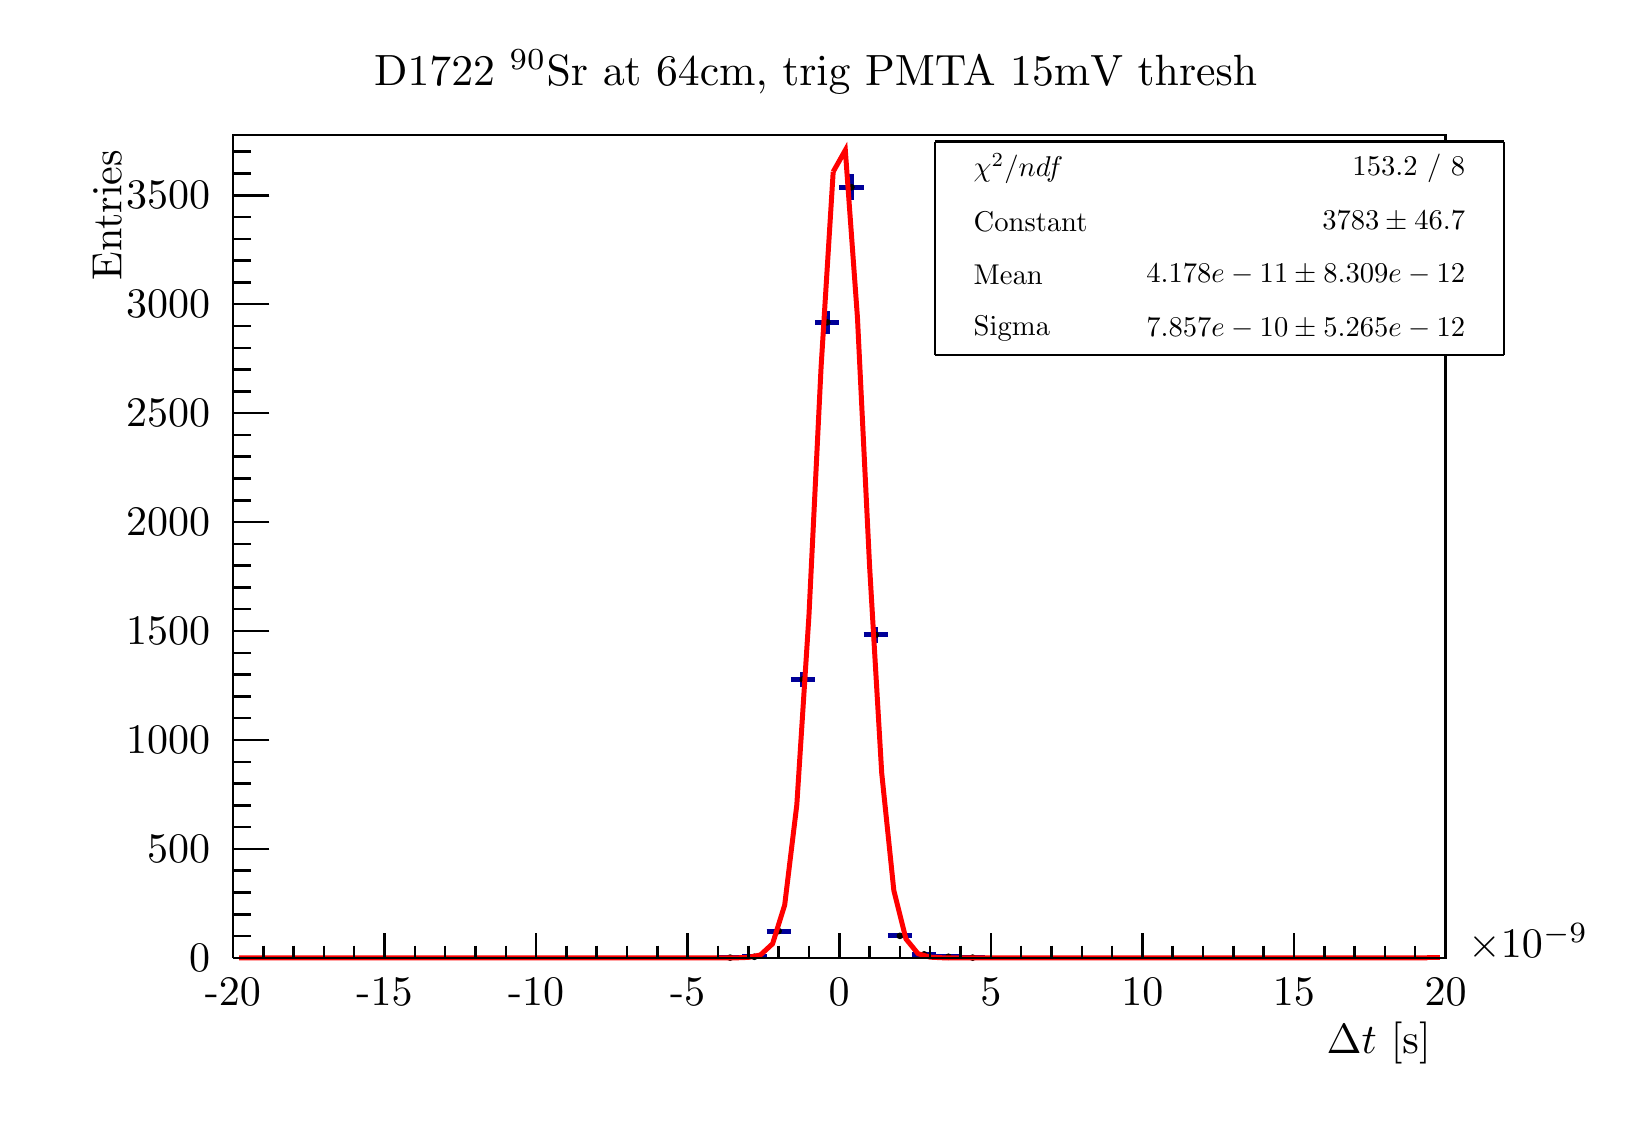
\begin{tikzpicture}
\pgfdeclareplotmark{cross} {
\pgfpathmoveto{\pgfpoint{-0.3\pgfplotmarksize}{\pgfplotmarksize}}
\pgfpathlineto{\pgfpoint{+0.3\pgfplotmarksize}{\pgfplotmarksize}}
\pgfpathlineto{\pgfpoint{+0.3\pgfplotmarksize}{0.3\pgfplotmarksize}}
\pgfpathlineto{\pgfpoint{+1\pgfplotmarksize}{0.3\pgfplotmarksize}}
\pgfpathlineto{\pgfpoint{+1\pgfplotmarksize}{-0.3\pgfplotmarksize}}
\pgfpathlineto{\pgfpoint{+0.3\pgfplotmarksize}{-0.3\pgfplotmarksize}}
\pgfpathlineto{\pgfpoint{+0.3\pgfplotmarksize}{-1.\pgfplotmarksize}}
\pgfpathlineto{\pgfpoint{-0.3\pgfplotmarksize}{-1.\pgfplotmarksize}}
\pgfpathlineto{\pgfpoint{-0.3\pgfplotmarksize}{-0.3\pgfplotmarksize}}
\pgfpathlineto{\pgfpoint{-1.\pgfplotmarksize}{-0.3\pgfplotmarksize}}
\pgfpathlineto{\pgfpoint{-1.\pgfplotmarksize}{0.3\pgfplotmarksize}}
\pgfpathlineto{\pgfpoint{-0.3\pgfplotmarksize}{0.3\pgfplotmarksize}}
\pgfpathclose
\pgfusepathqstroke
}
\pgfdeclareplotmark{cross*} {
\pgfpathmoveto{\pgfpoint{-0.3\pgfplotmarksize}{\pgfplotmarksize}}
\pgfpathlineto{\pgfpoint{+0.3\pgfplotmarksize}{\pgfplotmarksize}}
\pgfpathlineto{\pgfpoint{+0.3\pgfplotmarksize}{0.3\pgfplotmarksize}}
\pgfpathlineto{\pgfpoint{+1\pgfplotmarksize}{0.3\pgfplotmarksize}}
\pgfpathlineto{\pgfpoint{+1\pgfplotmarksize}{-0.3\pgfplotmarksize}}
\pgfpathlineto{\pgfpoint{+0.3\pgfplotmarksize}{-0.3\pgfplotmarksize}}
\pgfpathlineto{\pgfpoint{+0.3\pgfplotmarksize}{-1.\pgfplotmarksize}}
\pgfpathlineto{\pgfpoint{-0.3\pgfplotmarksize}{-1.\pgfplotmarksize}}
\pgfpathlineto{\pgfpoint{-0.3\pgfplotmarksize}{-0.3\pgfplotmarksize}}
\pgfpathlineto{\pgfpoint{-1.\pgfplotmarksize}{-0.3\pgfplotmarksize}}
\pgfpathlineto{\pgfpoint{-1.\pgfplotmarksize}{0.3\pgfplotmarksize}}
\pgfpathlineto{\pgfpoint{-0.3\pgfplotmarksize}{0.3\pgfplotmarksize}}
\pgfpathclose
\pgfusepathqfillstroke
}
\pgfdeclareplotmark{newstar} {
\pgfpathmoveto{\pgfqpoint{0pt}{\pgfplotmarksize}}
\pgfpathlineto{\pgfqpointpolar{44}{0.5\pgfplotmarksize}}
\pgfpathlineto{\pgfqpointpolar{18}{\pgfplotmarksize}}
\pgfpathlineto{\pgfqpointpolar{-20}{0.5\pgfplotmarksize}}
\pgfpathlineto{\pgfqpointpolar{-54}{\pgfplotmarksize}}
\pgfpathlineto{\pgfqpointpolar{-90}{0.5\pgfplotmarksize}}
\pgfpathlineto{\pgfqpointpolar{234}{\pgfplotmarksize}}
\pgfpathlineto{\pgfqpointpolar{198}{0.5\pgfplotmarksize}}
\pgfpathlineto{\pgfqpointpolar{162}{\pgfplotmarksize}}
\pgfpathlineto{\pgfqpointpolar{134}{0.5\pgfplotmarksize}}
\pgfpathclose
\pgfusepathqstroke
}
\pgfdeclareplotmark{newstar*} {
\pgfpathmoveto{\pgfqpoint{0pt}{\pgfplotmarksize}}
\pgfpathlineto{\pgfqpointpolar{44}{0.5\pgfplotmarksize}}
\pgfpathlineto{\pgfqpointpolar{18}{\pgfplotmarksize}}
\pgfpathlineto{\pgfqpointpolar{-20}{0.5\pgfplotmarksize}}
\pgfpathlineto{\pgfqpointpolar{-54}{\pgfplotmarksize}}
\pgfpathlineto{\pgfqpointpolar{-90}{0.5\pgfplotmarksize}}
\pgfpathlineto{\pgfqpointpolar{234}{\pgfplotmarksize}}
\pgfpathlineto{\pgfqpointpolar{198}{0.5\pgfplotmarksize}}
\pgfpathlineto{\pgfqpointpolar{162}{\pgfplotmarksize}}
\pgfpathlineto{\pgfqpointpolar{134}{0.5\pgfplotmarksize}}
\pgfpathclose
\pgfusepathqfillstroke
}
\definecolor{c}{rgb}{1,1,1};
\draw [color=c, fill=c] (0,0) rectangle (20,13.5705);
\draw [color=c, fill=c] (2.6,1.76416) rectangle (18,12.2134);
\definecolor{c}{rgb}{0,0,0};
\draw [c,line width=0.9] (2.6,1.76416) -- (2.6,12.2134) -- (18,12.2134) -- (18,1.76416) -- (2.6,1.76416);
\definecolor{c}{rgb}{1,1,1};
\draw [color=c, fill=c] (2.6,1.76416) rectangle (18,12.2134);
\definecolor{c}{rgb}{0,0,0};
\draw [c,line width=0.9] (2.6,1.76416) -- (2.6,12.2134) -- (18,12.2134) -- (18,1.76416) -- (2.6,1.76416);
\definecolor{c}{rgb}{0,0,0.6};
\draw [c,line width=1.8] (8.914,1.76416) -- (8.914,1.76693);
\draw [c,line width=1.8] (8.914,1.76693) -- (8.914,1.76969);
\draw [c,line width=1.8] (8.76,1.76693) -- (8.914,1.76693);
\draw [c,line width=1.8] (8.914,1.76693) -- (9.068,1.76693);
\definecolor{c}{rgb}{0,0,0};
\foreach \P in {(8.914,1.76693)}{\draw[mark options={color=c,fill=c},mark size=2.402402pt,mark=*,mark size=1pt] plot coordinates {\P};}
\definecolor{c}{rgb}{0,0,0.6};
\draw [c,line width=1.8] (9.222,1.77181) -- (9.222,1.77799);
\draw [c,line width=1.8] (9.222,1.77799) -- (9.222,1.78418);
\draw [c,line width=1.8] (9.068,1.77799) -- (9.222,1.77799);
\draw [c,line width=1.8] (9.222,1.77799) -- (9.376,1.77799);
\definecolor{c}{rgb}{0,0,0};
\foreach \P in {(9.222,1.77799)}{\draw[mark options={color=c,fill=c},mark size=2.402402pt,mark=*,mark size=1pt] plot coordinates {\P};}
\definecolor{c}{rgb}{0,0,0.6};
\draw [c,line width=1.8] (9.53,2.07382) -- (9.53,2.10451);
\draw [c,line width=1.8] (9.53,2.10451) -- (9.53,2.1352);
\draw [c,line width=1.8] (9.376,2.10451) -- (9.53,2.10451);
\draw [c,line width=1.8] (9.53,2.10451) -- (9.684,2.10451);
\definecolor{c}{rgb}{0,0,0};
\foreach \P in {(9.53,2.10451)}{\draw[mark options={color=c,fill=c},mark size=2.402402pt,mark=*,mark size=1pt] plot coordinates {\P};}
\definecolor{c}{rgb}{0,0,0.6};
\draw [c,line width=1.8] (9.838,5.20154) -- (9.838,5.30046);
\draw [c,line width=1.8] (9.838,5.30046) -- (9.838,5.39938);
\draw [c,line width=1.8] (9.684,5.30046) -- (9.838,5.30046);
\draw [c,line width=1.8] (9.838,5.30046) -- (9.992,5.30046);
\definecolor{c}{rgb}{0,0,0};
\foreach \P in {(9.838,5.30046)}{\draw[mark options={color=c,fill=c},mark size=2.402402pt,mark=*,mark size=1pt] plot coordinates {\P};}
\definecolor{c}{rgb}{0,0,0.6};
\draw [c,line width=1.8] (10.146,9.68623) -- (10.146,9.83568);
\draw [c,line width=1.8] (10.146,9.83568) -- (10.146,9.98513);
\draw [c,line width=1.8] (9.992,9.83568) -- (10.146,9.83568);
\draw [c,line width=1.8] (10.146,9.83568) -- (10.3,9.83568);
\definecolor{c}{rgb}{0,0,0};
\foreach \P in {(10.146,9.83568)}{\draw[mark options={color=c,fill=c},mark size=2.402402pt,mark=*,mark size=1pt] plot coordinates {\P};}
\definecolor{c}{rgb}{0,0,0.6};
\draw [c,line width=1.8] (10.454,11.3867) -- (10.454,11.5513);
\draw [c,line width=1.8] (10.454,11.5513) -- (10.454,11.7158);
\draw [c,line width=1.8] (10.3,11.5513) -- (10.454,11.5513);
\draw [c,line width=1.8] (10.454,11.5513) -- (10.608,11.5513);
\definecolor{c}{rgb}{0,0,0};
\foreach \P in {(10.454,11.5513)}{\draw[mark options={color=c,fill=c},mark size=2.402402pt,mark=*,mark size=1pt] plot coordinates {\P};}
\definecolor{c}{rgb}{0,0,0.6};
\draw [c,line width=1.8] (10.762,5.75842) -- (10.762,5.86495);
\draw [c,line width=1.8] (10.762,5.86495) -- (10.762,5.97147);
\draw [c,line width=1.8] (10.608,5.86495) -- (10.762,5.86495);
\draw [c,line width=1.8] (10.762,5.86495) -- (10.916,5.86495);
\definecolor{c}{rgb}{0,0,0};
\foreach \P in {(10.762,5.86495)}{\draw[mark options={color=c,fill=c},mark size=2.402402pt,mark=*,mark size=1pt] plot coordinates {\P};}
\definecolor{c}{rgb}{0,0,0.6};
\draw [c,line width=1.8] (11.07,2.01582) -- (11.07,2.04363);
\draw [c,line width=1.8] (11.07,2.04363) -- (11.07,2.07144);
\draw [c,line width=1.8] (10.916,2.04363) -- (11.07,2.04363);
\draw [c,line width=1.8] (11.07,2.04363) -- (11.224,2.04363);
\definecolor{c}{rgb}{0,0,0};
\foreach \P in {(11.07,2.04363)}{\draw[mark options={color=c,fill=c},mark size=2.402402pt,mark=*,mark size=1pt] plot coordinates {\P};}
\definecolor{c}{rgb}{0,0,0.6};
\draw [c,line width=1.8] (11.378,1.79736) -- (11.378,1.80843);
\draw [c,line width=1.8] (11.378,1.80843) -- (11.378,1.8195);
\draw [c,line width=1.8] (11.224,1.80843) -- (11.378,1.80843);
\draw [c,line width=1.8] (11.378,1.80843) -- (11.532,1.80843);
\definecolor{c}{rgb}{0,0,0};
\foreach \P in {(11.378,1.80843)}{\draw[mark options={color=c,fill=c},mark size=2.402402pt,mark=*,mark size=1pt] plot coordinates {\P};}
\definecolor{c}{rgb}{0,0,0.6};
\draw [c,line width=1.8] (11.686,1.77181) -- (11.686,1.77799);
\draw [c,line width=1.8] (11.686,1.77799) -- (11.686,1.78418);
\draw [c,line width=1.8] (11.532,1.77799) -- (11.686,1.77799);
\draw [c,line width=1.8] (11.686,1.77799) -- (11.84,1.77799);
\definecolor{c}{rgb}{0,0,0};
\foreach \P in {(11.686,1.77799)}{\draw[mark options={color=c,fill=c},mark size=2.402402pt,mark=*,mark size=1pt] plot coordinates {\P};}
\definecolor{c}{rgb}{0,0,0.6};
\draw [c,line width=1.8] (11.994,1.76416) -- (11.994,1.76693);
\draw [c,line width=1.8] (11.994,1.76693) -- (11.994,1.76969);
\draw [c,line width=1.8] (11.84,1.76693) -- (11.994,1.76693);
\draw [c,line width=1.8] (11.994,1.76693) -- (12.148,1.76693);
\definecolor{c}{rgb}{0,0,0};
\foreach \P in {(11.994,1.76693)}{\draw[mark options={color=c,fill=c},mark size=2.402402pt,mark=*,mark size=1pt] plot coordinates {\P};}
\definecolor{c}{rgb}{1,0,0};
\draw [c,line width=1.8] (2.677,1.76416) -- (2.831,1.76416) -- (2.985,1.76416) -- (3.139,1.76416) -- (3.293,1.76416) -- (3.447,1.76416) -- (3.601,1.76416) -- (3.755,1.76416) -- (3.909,1.76416) -- (4.063,1.76416) -- (4.217,1.76416) -- (4.371,1.76416)
 -- (4.525,1.76416) -- (4.679,1.76416) -- (4.833,1.76416) -- (4.987,1.76416) -- (5.141,1.76416) -- (5.295,1.76416) -- (5.449,1.76416) -- (5.603,1.76416) -- (5.757,1.76416) -- (5.911,1.76416) -- (6.065,1.76416) -- (6.219,1.76416) -- (6.373,1.76416) --
 (6.527,1.76416) -- (6.681,1.76416) -- (6.835,1.76416) -- (6.989,1.76416) -- (7.143,1.76416) -- (7.297,1.76416) -- (7.451,1.76416) -- (7.605,1.76416) -- (7.759,1.76416) -- (7.913,1.76416) -- (8.067,1.76416) -- (8.221,1.76416) -- (8.375,1.76416) --
 (8.529,1.76416) -- (8.683,1.76416) -- (8.837,1.76416) -- (8.991,1.76416) -- (9.145,1.76998) -- (9.299,1.80089) -- (9.453,1.94285) -- (9.607,2.43506) -- (9.761,3.70796) -- (9.915,6.11015) -- (10.069,9.26248) -- (10.223,11.7476);
\draw [c,line width=1.8] (10.223,11.7476) -- (10.377,12.0215) -- (10.531,9.89679) -- (10.685,6.74) -- (10.839,4.11347) -- (10.993,2.62012) -- (11.147,2.00482) -- (11.301,1.81637) -- (11.455,1.7729) -- (11.609,1.76529) -- (11.763,1.76416) --
 (11.917,1.76416) -- (12.071,1.76416) -- (12.225,1.76416) -- (12.379,1.76416) -- (12.533,1.76416) -- (12.687,1.76416) -- (12.841,1.76416) -- (12.995,1.76416) -- (13.149,1.76416) -- (13.303,1.76416) -- (13.457,1.76416) -- (13.611,1.76416) --
 (13.765,1.76416) -- (13.919,1.76416) -- (14.073,1.76416) -- (14.227,1.76416) -- (14.381,1.76416) -- (14.535,1.76416) -- (14.689,1.76416) -- (14.843,1.76416) -- (14.997,1.76416) -- (15.151,1.76416) -- (15.305,1.76416) -- (15.459,1.76416) --
 (15.613,1.76416) -- (15.767,1.76416) -- (15.921,1.76416) -- (16.075,1.76416) -- (16.229,1.76416) -- (16.383,1.76416) -- (16.537,1.76416) -- (16.691,1.76416) -- (16.845,1.76416) -- (16.999,1.76416) -- (17.153,1.76416) -- (17.307,1.76416) --
 (17.461,1.76416) -- (17.615,1.76416) -- (17.769,1.76416);
\draw [c,line width=1.8] (17.769,1.76416) -- (17.923,1.76416);
\definecolor{c}{rgb}{1,1,1};
\draw [color=c, fill=c] (11.5186,9.42152) rectangle (18.7393,12.1299);
\definecolor{c}{rgb}{0,0,0};
\draw [c,line width=0.9] (11.5186,9.42152) -- (18.7393,9.42152);
\draw [c,line width=0.9] (18.7393,9.42152) -- (18.7393,12.1299);
\draw [c,line width=0.9] (18.7393,12.1299) -- (11.5186,12.1299);
\draw [c,line width=0.9] (11.5186,12.1299) -- (11.5186,9.42152);
\draw [anchor= west] (11.8797,11.7913) node[scale=1.03301, color=c, rotate=0]{$\chi^{2} / ndf $};
\draw [anchor= east] (18.3782,11.7913) node[scale=1.03301, color=c, rotate=0]{ 153.2 / 8};
\draw [anchor= west] (11.8797,11.1142) node[scale=1.03301, color=c, rotate=0]{Constant };
\draw [anchor= east] (18.3782,11.1142) node[scale=1.03301, color=c, rotate=0]{$  3783 \pm 46.7$};
\draw [anchor= west] (11.8797,10.4371) node[scale=1.03301, color=c, rotate=0]{Mean     };
\draw [anchor= east] (18.3782,10.4371) node[scale=1.03301, color=c, rotate=0]{$ 4.178e-11 \pm 8.309e-12$};
\draw [anchor= west] (11.8797,9.76007) node[scale=1.03301, color=c, rotate=0]{Sigma    };
\draw [anchor= east] (18.3782,9.76007) node[scale=1.03301, color=c, rotate=0]{$ 7.857e-10 \pm 5.265e-12$};
\draw [c,line width=0.9] (2.6,1.76416) -- (18,1.76416);
\draw [c,line width=0.9] (2.6,2.07764) -- (2.6,1.76416);
\draw [c,line width=0.9] (2.985,1.9209) -- (2.985,1.76416);
\draw [c,line width=0.9] (3.37,1.9209) -- (3.37,1.76416);
\draw [c,line width=0.9] (3.755,1.9209) -- (3.755,1.76416);
\draw [c,line width=0.9] (4.14,1.9209) -- (4.14,1.76416);
\draw [c,line width=0.9] (4.525,2.07764) -- (4.525,1.76416);
\draw [c,line width=0.9] (4.91,1.9209) -- (4.91,1.76416);
\draw [c,line width=0.9] (5.295,1.9209) -- (5.295,1.76416);
\draw [c,line width=0.9] (5.68,1.9209) -- (5.68,1.76416);
\draw [c,line width=0.9] (6.065,1.9209) -- (6.065,1.76416);
\draw [c,line width=0.9] (6.45,2.07764) -- (6.45,1.76416);
\draw [c,line width=0.9] (6.835,1.9209) -- (6.835,1.76416);
\draw [c,line width=0.9] (7.22,1.9209) -- (7.22,1.76416);
\draw [c,line width=0.9] (7.605,1.9209) -- (7.605,1.76416);
\draw [c,line width=0.9] (7.99,1.9209) -- (7.99,1.76416);
\draw [c,line width=0.9] (8.375,2.07764) -- (8.375,1.76416);
\draw [c,line width=0.9] (8.76,1.9209) -- (8.76,1.76416);
\draw [c,line width=0.9] (9.145,1.9209) -- (9.145,1.76416);
\draw [c,line width=0.9] (9.53,1.9209) -- (9.53,1.76416);
\draw [c,line width=0.9] (9.915,1.9209) -- (9.915,1.76416);
\draw [c,line width=0.9] (10.3,2.07764) -- (10.3,1.76416);
\draw [c,line width=0.9] (10.685,1.9209) -- (10.685,1.76416);
\draw [c,line width=0.9] (11.07,1.9209) -- (11.07,1.76416);
\draw [c,line width=0.9] (11.455,1.9209) -- (11.455,1.76416);
\draw [c,line width=0.9] (11.84,1.9209) -- (11.84,1.76416);
\draw [c,line width=0.9] (12.225,2.07764) -- (12.225,1.76416);
\draw [c,line width=0.9] (12.61,1.9209) -- (12.61,1.76416);
\draw [c,line width=0.9] (12.995,1.9209) -- (12.995,1.76416);
\draw [c,line width=0.9] (13.38,1.9209) -- (13.38,1.76416);
\draw [c,line width=0.9] (13.765,1.9209) -- (13.765,1.76416);
\draw [c,line width=0.9] (14.15,2.07764) -- (14.15,1.76416);
\draw [c,line width=0.9] (14.535,1.9209) -- (14.535,1.76416);
\draw [c,line width=0.9] (14.92,1.9209) -- (14.92,1.76416);
\draw [c,line width=0.9] (15.305,1.9209) -- (15.305,1.76416);
\draw [c,line width=0.9] (15.69,1.9209) -- (15.69,1.76416);
\draw [c,line width=0.9] (16.075,2.07764) -- (16.075,1.76416);
\draw [c,line width=0.9] (16.46,1.9209) -- (16.46,1.76416);
\draw [c,line width=0.9] (16.845,1.9209) -- (16.845,1.76416);
\draw [c,line width=0.9] (17.23,1.9209) -- (17.23,1.76416);
\draw [c,line width=0.9] (17.615,1.9209) -- (17.615,1.76416);
\draw [c,line width=0.9] (18,2.07764) -- (18,1.76416);
\draw [anchor=base] (2.6,1.15349) node[scale=1.51913, color=c, rotate=0]{-20};
\draw [anchor=base] (4.525,1.15349) node[scale=1.51913, color=c, rotate=0]{-15};
\draw [anchor=base] (6.45,1.15349) node[scale=1.51913, color=c, rotate=0]{-10};
\draw [anchor=base] (8.375,1.15349) node[scale=1.51913, color=c, rotate=0]{-5};
\draw [anchor=base] (10.3,1.15349) node[scale=1.51913, color=c, rotate=0]{0};
\draw [anchor=base] (12.225,1.15349) node[scale=1.51913, color=c, rotate=0]{5};
\draw [anchor=base] (14.15,1.15349) node[scale=1.51913, color=c, rotate=0]{10};
\draw [anchor=base] (16.075,1.15349) node[scale=1.51913, color=c, rotate=0]{15};
\draw [anchor=base] (18,1.15349) node[scale=1.51913, color=c, rotate=0]{20};
\draw [anchor=base west] (18.1,1.76416) node[scale=1.51913, color=c, rotate=0]{$\times10^{-9}$};
\draw [anchor= east] (18,0.678523) node[scale=1.51913, color=c, rotate=0]{$\Delta t$ [s]};
\draw [c,line width=0.9] (2.6,1.76416) -- (2.6,12.2134);
\draw [c,line width=0.9] (3.062,1.76416) -- (2.6,1.76416);
\draw [c,line width=0.9] (2.831,2.04086) -- (2.6,2.04086);
\draw [c,line width=0.9] (2.831,2.31757) -- (2.6,2.31757);
\draw [c,line width=0.9] (2.831,2.59428) -- (2.6,2.59428);
\draw [c,line width=0.9] (2.831,2.87098) -- (2.6,2.87098);
\draw [c,line width=0.9] (3.062,3.14769) -- (2.6,3.14769);
\draw [c,line width=0.9] (2.831,3.4244) -- (2.6,3.4244);
\draw [c,line width=0.9] (2.831,3.7011) -- (2.6,3.7011);
\draw [c,line width=0.9] (2.831,3.97781) -- (2.6,3.97781);
\draw [c,line width=0.9] (2.831,4.25451) -- (2.6,4.25451);
\draw [c,line width=0.9] (3.062,4.53122) -- (2.6,4.53122);
\draw [c,line width=0.9] (2.831,4.80793) -- (2.6,4.80793);
\draw [c,line width=0.9] (2.831,5.08463) -- (2.6,5.08463);
\draw [c,line width=0.9] (2.831,5.36134) -- (2.6,5.36134);
\draw [c,line width=0.9] (2.831,5.63805) -- (2.6,5.63805);
\draw [c,line width=0.9] (3.062,5.91475) -- (2.6,5.91475);
\draw [c,line width=0.9] (2.831,6.19146) -- (2.6,6.19146);
\draw [c,line width=0.9] (2.831,6.46816) -- (2.6,6.46816);
\draw [c,line width=0.9] (2.831,6.74487) -- (2.6,6.74487);
\draw [c,line width=0.9] (2.831,7.02158) -- (2.6,7.02158);
\draw [c,line width=0.9] (3.062,7.29828) -- (2.6,7.29828);
\draw [c,line width=0.9] (2.831,7.57499) -- (2.6,7.57499);
\draw [c,line width=0.9] (2.831,7.8517) -- (2.6,7.8517);
\draw [c,line width=0.9] (2.831,8.1284) -- (2.6,8.1284);
\draw [c,line width=0.9] (2.831,8.40511) -- (2.6,8.40511);
\draw [c,line width=0.9] (3.062,8.68182) -- (2.6,8.68182);
\draw [c,line width=0.9] (2.831,8.95852) -- (2.6,8.95852);
\draw [c,line width=0.9] (2.831,9.23523) -- (2.6,9.23523);
\draw [c,line width=0.9] (2.831,9.51193) -- (2.6,9.51193);
\draw [c,line width=0.9] (2.831,9.78864) -- (2.6,9.78864);
\draw [c,line width=0.9] (3.062,10.0653) -- (2.6,10.0653);
\draw [c,line width=0.9] (2.831,10.3421) -- (2.6,10.3421);
\draw [c,line width=0.9] (2.831,10.6188) -- (2.6,10.6188);
\draw [c,line width=0.9] (2.831,10.8955) -- (2.6,10.8955);
\draw [c,line width=0.9] (2.831,11.1722) -- (2.6,11.1722);
\draw [c,line width=0.9] (3.062,11.4489) -- (2.6,11.4489);
\draw [c,line width=0.9] (3.062,11.4489) -- (2.6,11.4489);
\draw [c,line width=0.9] (2.831,11.7256) -- (2.6,11.7256);
\draw [c,line width=0.9] (2.831,12.0023) -- (2.6,12.0023);
\draw [anchor= east] (2.5,1.76416) node[scale=1.51913, color=c, rotate=0]{0};
\draw [anchor= east] (2.5,3.14769) node[scale=1.51913, color=c, rotate=0]{500};
\draw [anchor= east] (2.5,4.53122) node[scale=1.51913, color=c, rotate=0]{1000};
\draw [anchor= east] (2.5,5.91475) node[scale=1.51913, color=c, rotate=0]{1500};
\draw [anchor= east] (2.5,7.29828) node[scale=1.51913, color=c, rotate=0]{2000};
\draw [anchor= east] (2.5,8.68182) node[scale=1.51913, color=c, rotate=0]{2500};
\draw [anchor= east] (2.5,10.0653) node[scale=1.51913, color=c, rotate=0]{3000};
\draw [anchor= east] (2.5,11.4489) node[scale=1.51913, color=c, rotate=0]{3500};
\draw [anchor= east] (1,12.2134) node[scale=1.51913, color=c, rotate=90]{Entries};
\definecolor{c}{rgb}{1,1,1};
\draw [color=c, fill=c] (11.5186,9.42152) rectangle (18.7393,12.1299);
\definecolor{c}{rgb}{0,0,0};
\draw [c,line width=0.9] (11.5186,9.42152) -- (18.7393,9.42152);
\draw [c,line width=0.9] (18.7393,9.42152) -- (18.7393,12.1299);
\draw [c,line width=0.9] (18.7393,12.1299) -- (11.5186,12.1299);
\draw [c,line width=0.9] (11.5186,12.1299) -- (11.5186,9.42152);
\draw [anchor= west] (11.8797,11.7913) node[scale=1.03301, color=c, rotate=0]{$\chi^{2} / ndf $};
\draw [anchor= east] (18.3782,11.7913) node[scale=1.03301, color=c, rotate=0]{ 153.2 / 8};
\draw [anchor= west] (11.8797,11.1142) node[scale=1.03301, color=c, rotate=0]{Constant };
\draw [anchor= east] (18.3782,11.1142) node[scale=1.03301, color=c, rotate=0]{$  3783 \pm 46.7$};
\draw [anchor= west] (11.8797,10.4371) node[scale=1.03301, color=c, rotate=0]{Mean     };
\draw [anchor= east] (18.3782,10.4371) node[scale=1.03301, color=c, rotate=0]{$ 4.178e-11 \pm 8.309e-12$};
\draw [anchor= west] (11.8797,9.76007) node[scale=1.03301, color=c, rotate=0]{Sigma    };
\draw [anchor= east] (18.3782,9.76007) node[scale=1.03301, color=c, rotate=0]{$ 7.857e-10 \pm 5.265e-12$};
\draw (10,13.0186) node[scale=1.5799, color=c, rotate=0]{D1722 $^{90}$Sr at 64cm, trig PMTA 15mV thresh};
\end{tikzpicture}

  \end{adjustbox}
  \caption{Difference in signal arrival time PMTs at each end of a bar as measured using a $^{90}$Sr source placed 64~cm from one end of the bar.}
  \label{fig:s4Res}	
\end{figure}

\begin{figure}[ht]    
  \centering
  \includegraphics[width=0.5\linewidth]{files/Figures/dstofFront2.png}
  \hfill
  \includegraphics[width=0.35\linewidth]{files/Figures/dstofDiag2.png}
  \caption{Front (left) and rotated (right) view of the $\mathit{S4}$. The rotated view shows more clearly the staggering of the scintillator bars and PMTs.}
  \label{fig:dstofDiagram}
\end{figure}

The anode signals of all 20 of the PMTs are discriminated using LeCroy 620AL NIM discriminators, at a threshold of 20~mV.
The discriminated signals are then fed into a time-to-digital converter (TDC). A signal in $\mathit{S4}$ is deemed to have occurred if a signal is seen in both PMTs, above the discriminator threshold, on the same bar within 20~ns of each other. 
This timing window is determined through testing performed with a $^{90}$Sr source at known positions on the bar.

The $\mathit{S1-S2}$ coincidence signal is digitized by the same TDC. This signal is used to calculate the particle time of flight from $\mathit{S2}$ to $\mathit{S4}$.

\subsection{The HPTPC Prototype}
For the characterisation of the beam using the ToF systems described in this paper, the relevant characteristics of the HPTPC prototype are the location and thickness of the steel vessel walls.
The cylindrical steel vessel has a 142~cm outer diameter; the main body is 60 cm in length and the rounded end caps protrude an additional 37~cm on each end.
With 1~cm thick walls it is rated to 6~barA of pressure.
The vessel wall thickness is equivalent to the range of a proton with a kinetic energy of approximately 80~MeV~\cite{rangeTables}.
The angular position of the center of the TPC is approximately $\theta = -2.5^{\circ}$. 
More details of the position and extent of the TPC are given in Table~\ref{tab:angS1} and Table~\ref{tab:distances}.
 
The active TPC is a cylinder, 111~cm in diameter and 48~cm in length; the TPC comprised thin steel mesh electrodes (one cathode and three anodes), and 12 copper rings to create the uniform drift field. The anodes were supported by a hexagonal aluminium stiffener on the side facing away from the camera.
Data taking with the TPC made use of both optical and charge readout.
The vessel, electrodes, and drift region of the TPC are shown in Figure~\ref{fig:TPC}.

\begin{figure}
  \centering
  \includegraphics[width=.88\linewidth]{files/Figures/vesselView.pdf}
  \caption{Cross-sectional view of the TPC; the thin mesh electrodes and copper ring drift volume can be seen inside the steel vessel. The walls of the vessel shown are 1~cm thick with a vessel outer diameter of 142~cm. At the point of hitting the vessel, the beam centre was 1~cm below the centre of the vessel vertically, where the distance from the inside of the vessel wall to the drift region was 15~cm.}
   \label{fig:TPC}
   %Vessel: wall thickness 1cm, beam centre height -1.14cm, 
\end{figure}

Throughout the run, the TPC was filled with either pure argon, or a combination of argon and a small percentage of quencher.
The performance of this TPC is the subject of a forthcoming publication~\cite{Deisting:2020aaa}.
